%% uctest.tex 11/3/94
%% Copyright (C) 1988-2004 Daniel Gildea, BBF, Ethan Munson.
%
% This work may be distributed and/or modified under the
% conditions of the LaTeX Project Public License, either version 1.3
% of this license or (at your option) any later version.
% The latest version of this license is in
%   http://www.latex-project.org/lppl.txt
% and version 1.3 or later is part of all distributions of LaTeX
% version 2003/12/01 or later.
%
% This work has the LPPL maintenance status "maintained".
% 
% The Current Maintainer of this work is Daniel Gildea.

\documentclass[11pt]{ucthesis}
\def\dsp{\def\baselinestretch{2.0}\large\normalsize}
\dsp

% 2010june01 sol katzman:
% package geometry should override the various margin settings from .clo and .cls
% and also eliminates issues where the default papersize is A4
\usepackage[letterpaper, left=1.5in, right=1.25in, top=1.25in, bottom=1.25in, includefoot]{geometry}
% Use PostScript fonts as required by UCSC Dissertation Preparation Guidelines 
\usepackage{pslatex}
\usepackage[utf8]{inputenc}
\usepackage{amssymb}
\usepackage{amsmath}
\usepackage{graphicx,subfigure}
\usepackage{multirow}
\usepackage{todonotes}
\usepackage{url}
\usepackage{soul}
\usepackage{xcolor}
\usepackage{xr}
\usepackage{float}
\usepackage{cite}
\usepackage{xspace} 
\usepackage{booktabs}
\usepackage[singlelinecheck=false,labelfont=bf]{caption}
\usepackage[linesnumbered,ruled,vlined]{algorithm2e}
\usepackage{epstopdf}
\usepackage{algorithmicx}
\usepackage[noend]{algpseudocode}
\usepackage{marvosym}
\usepackage{booktabs} 
\usepackage{lipsum}
\usepackage{ntheorem}
\usepackage{makecell}
  
\setlength{\tabcolsep}{8pt}
\renewcommand{\arraystretch}{1.25}

\usepackage{array}
\newcolumntype{L}[1]{>{\raggedright\let\newline\\\arraybackslash\hspace{0pt}}m{#1}}
\newcolumntype{C}[1]{>{\centering\let\newline\\\arraybackslash\hspace{0pt}}m{#1}}
\newcolumntype{R}[1]{>{\raggedleft\let\newline\\\arraybackslash\hspace{0pt}}m{#1}}

\newcommand{\tool}[1]{\emph{\textsc{#1}}}
\newcommand{\figref}[1]{Fig. \ref{fig:#1}}
\newcommand{\vocab}{\textbf}

\newtheorem{theorem}{Theorem}
\newtheorem{lemma}{Lemma}
\newtheorem{corollary}[lemma]{Corollary}
\newtheorem*{proof}{Proof}

\begin{document}

% Declarations for Front Matter

\title{Graph methods for computational pangenomics}
\author{Jordan M Eizenga}
\degreeyear{2021}
\degreemonth{June}
\degree{DOCTOR OF PHILOSOPHY}
\chair{Professor Benedict Paten}
\committeememberone{Professor David Haussler}
\committeemembertwo{Professor R. Edward Green}
%\committeememberthree{Professor Ipsum Lorem}
\numberofmembers{3} %% (including chair) possible: 3, 4, 5, 6
\deanlineone{Dean Peter F. Biehl}
\deanlinetwo{Vice Provost and Dean of Graduate Studies}
\deanlinethree{}
\field{Bioinformatics}
\campus{Santa Cruz}

\begin{frontmatter}

\maketitle
\copyrightpage

\tableofcontents
\listoffigures
\listoftables

\begin{abstract}

In most sequencing experiments, sequencing reads are mapped to a reference genome assembly in order to identify the genomic elements that the reads originated from. The mapping process becomes less accurate when the sample's genome differs from the reference genome. This introduces a pervasive \emph{reference bias} in which genomics analyses are systematically less accurate for non-reference alleles. In the field of pangenomics, it has been proposed that more general reference structures could mitigate reference bias. The fundamental idea is to incorporate population variation into the reference itself. The result is naturally expressible as a sequence graph. This dissertation presents the research I performed to develop methods for graph-based pangenomic analyses. First, I describe a read mapping and inference pipeline to perform haplotype-resolve transcriptomic analyses using pangenomics techniques. Next, I describe several contributions I have made to the ecosystem of pangenomic software: an interface to conventional reference methods, a software library of pangenome graph data structures, and a usable interface for indexing pangenome graphs. Finally, I describe some applications of graph theory to pangenome graphs to perform practical pangenomics tasks: identifying sites of variation and converting overlapped sequence graphs to blunt ones.

\end{abstract}

\begin{dedication}
\null\vfil
{\large
\begin{center}
To my parents,\\%\vspace{12pt}
Douglas and Lori Eizenga,\\%\vspace{12pt}
who I can always count on, \\\vspace{48pt}
and to my dear friend, \\%\vspace{12pt}
Corrie Janssens,\\%\vspace{12pt}
my moral North Star
\end{center}}
\vfil\null
\end{dedication}


\begin{acknowledgements}

I would like to thank the members of my committee, Benedict Paten, David Haussler, and Ed Green for their insight and critique of the work presented in my dissertation and defense. I am particularly grateful to Benedict Paten for the years of mentorship he has provided me in the Computational Genomics Lab. His guidance taught me how to conduct science and led me to a challenging and rewarding area of study.

My lab mates have been my collaborators, commiserators, and friends. I am grateful to have worked alongside Art Rand, Miten Jain, Adam Novak, Glenn Hickey, John Vivan, Audrey Musselman-Brown, Trevor Peasout, Molly Zhang, Yohei Rosen, Xian Chang, Jouni Sir{\'e}n, Marina Haukness, Kishwar Shafin, Andrew Bailey, Colleen Bosworth, Ryan Lorig-Roach, Jean Monlong, Jonas Sibbesen, Robin Rounthwaite, James Casaletto, Yatish Turakhia, Melissa Meredith, Cecilia Cisar, and Mobin Asri. For the last six years, they have provided me with an intellectually stimulating environment and with a sense of community. Outside of my lab, I feel I should also specifically thank my friend and collaborator Erik Garrison, whose vision and leadership were motive forces in the research community I belong to.

The route I took into bioinformatics was rather circuitous. In my mind, the most crucial determinative period was my mid-twenties, when I was broke, depressed, and unable to work after developing a chronic medical condition. I ended up getting the lifeline I needed from the burgeoning availability of free online college-level educational materials. Engaging in these courses pulled me out of that slump and completely reshaped my interests, which is ultimately what led me to graduate school in bioinformatics. Because of this, I feel grateful to a number of professors I have never personally met, and who yet profoundly impacted my life. In particular, I would like to thank David J. Malan, Eric Lander, Pavel Pevzner, Phillip Compeau, Tim Roughgarden, Leonard E. White, Andrew Ng, Marnie Blewitt, Rob Tibshirani, Trevor Hastie, Eric Grimson, and Alma Novotny for their generosity with their time and expertise.

The University of California Santa Cruz has been my home for six years, and I am grateful to the people in the campus community who are working to make it a fairer and juster place. I want to thank the COLA wildcats for the risks they took and the sacrifices they made on behalf of all UCSC graduate students. I would particularly like to thank Carlos Cruz who continues to face unjust retaliation for his participation in the movement. The mobilization that the wildcats galvanized has borne further fruit in the Student Researchers United campaign, which I am proud to have been a part of. I am grateful for my fellow members of the organizing committee, as well as the 1000+ graduate students who have contributed to the campaign across the UC system.

Many more people have made the last six years of my life feel rich and meaningful. I am grateful for my community of friends, both in Santa Cruz and Michigan; I am grateful for my students, whose curiosity reinvigorates my own interest; I am grateful for and proud of the undergraduate researchers I have had the pleasure of mentoring; and I am grateful for the administrative staff who shepherded me through the whole process.

Finally and most of all, I would like to thank the members of my family. My mom and dad have supported my love of learning for my entire life. They have demonstrated over and over again that if I ever slip, someone will always be there to catch me. My brother Quentin's relentless enthusiasm and dedication inspired me to take the plunge into graduate school in the first place. My brother Nate's nerdiness and humor fits like a glove with my own. My dear friend Corrie, who I consider family, is my personal hero, and I am continually impressed with her wisdom and growth.

In sum, this thesis is very much a group project, but, as we all know, every group project has that one person who actually did all the work...  ;)

\end{acknowledgements}

\end{frontmatter}

\part{Introduction and background}

\chapter{Introduction}

\label{chapter:intro}

%Modern biologists can ask and answer a qualitatively greater set of questions at a quantitatively greater scale than their predecessors. Undergirding this expansion in capabilities is a deepened arsenal of technologies, and DNA sequencing is undoubtedly one of the most fundamental among them. The centrality of sequencing is due in part to the fundamental importance of DNA in biology; DNA is the (nearly) universal medium of heredity and the primary object of evolutionary change. In addition, DNA sequencing has proven to be highly adaptable for assaying various biological processes---many unbiased assays consist mainly in a method to imprint the effects of a process on DNA molecules, which is then followed by sequencing. %

Modern biologists can ask and answer a qualitatively greater set of questions at a quantitatively greater scale than their predecessors. Much of this expansion is reflected in the growing use of so-called \emph{omics} methods. This term cheekily refers to a variety of methods that attempt to characterize the entirety of some class of biomolecular entity in a sample: all DNA in genomics, all proteins in proteomics, all metabolites in metabolomics, etc. Earlier methods in molecular biology that focused on individual entities (e.g.\ one gene) sometimes suffered a tunnel vision that could seriously slant the scientific understanding of a biological process. The widened lens of omics methods alleviates this risk, and thus they are often referred to as \emph{unbiased} methods (although it may be more accurate to call them less-biased methods---more on this soon).

Undergirding the growth of omics methods is a deepened arsenal of technologies, and DNA sequencing is undoubtedly one of the most fundamental among them. The centrality of sequencing is due in part to the fundamental importance of DNA in biology; DNA is the (nearly) universal medium of heredity and the primary object of evolutionary change. In addition, DNA sequencing has proven to be highly adaptable for assaying various biological processes. Many unbiased assays consist mainly in a method to imprint the effects of some process onto DNA molecules, which is then followed by sequencing. 

The vast majority of sequencing experiments involve \emph{resequencing}: generating sequencing data from an organism for which some individual's genome has been previously sequenced and assembled. For humans and model species, the assembled genomes are maintained as high-quality public data resources, referred to as \emph{reference genomes}. In practice, this turns out to be crucial for two interrelated reasons. First, the reference serves as a technical tool to identify the genomic element corresponding to raw sequencing data. Second, the reference coordinate system acts as a proxy for homology between individual genomes. Together, these features allow sequencing experiments to be interpreted and generalized beyond the individual sample so that they can contribute to scientific understanding of biology.

Reference-based analysis is an expedient and well-developed methodology, but it does have downsides. For one, there is a fundamental limitation in using a single genome as a reference for an entire species. At best, a reference assembly can accurately represent the genomic sequence of a single haplotype of a single individual. Every other individual will have genetic differences so that their genome mismatches the reference in many locations. This introduces some ambiguity into the reference's role as a coordinate system. More subtly, it also diminishes the reference's ability to serve as a technical tool. The way that sequencing data is identified with a genomic element in the reference is by looking for sequences in the reference that match the data. If in fact the reference mismatches the genome that generated the data, it is more difficult to identify the correct element, and the accuracy of this process deteriorates. This problem is known as \emph{reference bias}: the systematic tendency for analyses to reduce in accuracy when a sample genome sequence differs from the reference. 

Recently, \emph{pangenomics} has emerged as a powerful methodology to mitigate these shortcomings. The core idea is to replace reference genomes with more general reference structures that incorporate genomic variation across individuals. Including alternate alleles in the reference structure eliminates the privileged role of the reference allele, which is what leads to reference bias. Various approaches for doing so have been proposed, the majority of which have been based on \emph{sequence graphs} (Figure \ref{fig:graph_example}). These graphs consist of vertices labeled with DNA sequences, which are connected by edges that indicate adjacency within a single DNA molecule. This structure allows sequences to split and rejoin around sites of variation. A full genome sequence can then be formed by concatenating sequences along a walk through a graph. In this way, the graph encodes a space of sequences rather than a single genome sequence.

\begin{figure}[h]
\begin{center}
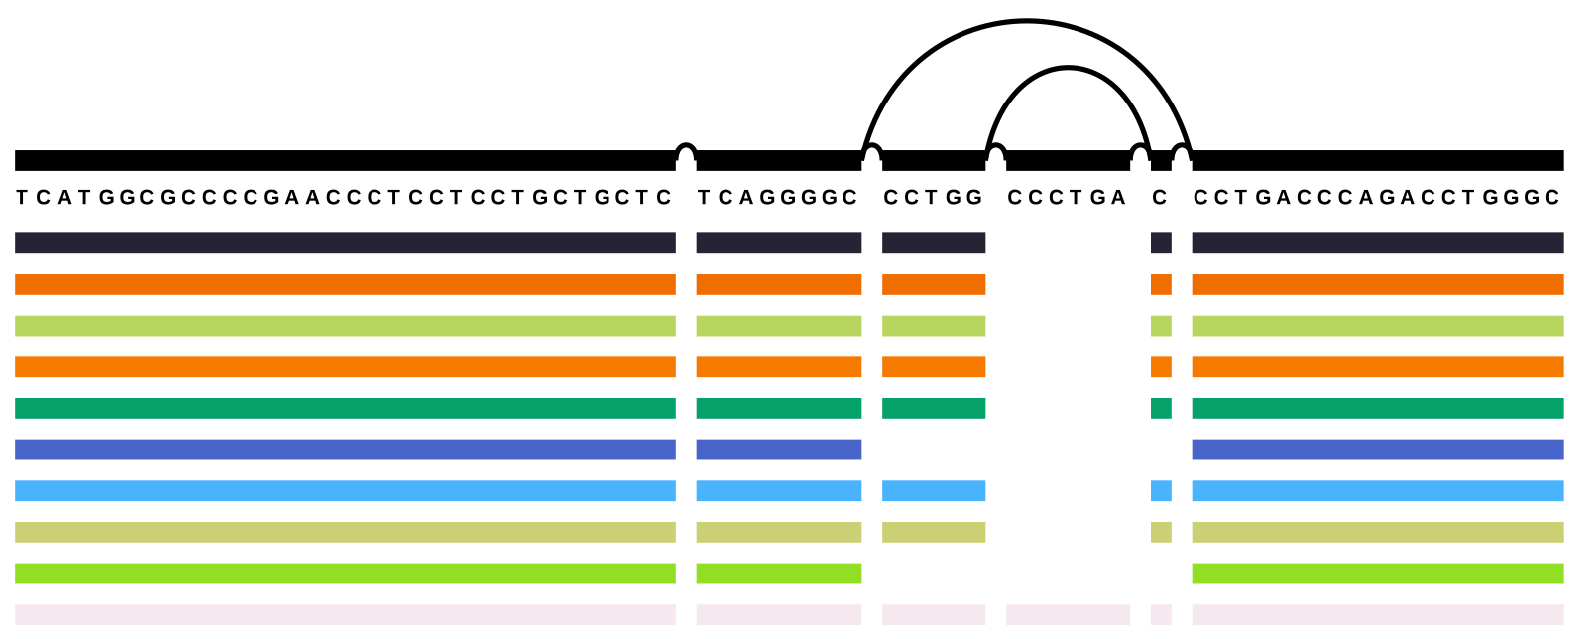
\includegraphics[width=.75\textwidth]{introfigures/pangenome_graph.png}
\caption{\textbf{An example of a sequence graph.} Colored bars indicate the walk taken by several haplotypes through the graph. The sequence of each haplotype can be reconstructed by concatenating the labels of the DNA sequences along the walk. Figure adapted from \cite{Garrison_2019}.
} \label{fig:graph_example}
\end{center}
\end{figure}

My thesis research has centered on developing methods for graph-based pangenomic analysis. Taken as a whole, the pangenomics project is rather ambitious. Reference genomes occupy a central role in genomics. Changing this core underlying formalism requires virtually every aspect of genomics analysis to be reconsidered, redesigned, and reimplemented. For this reason, it has been very satisfying to see field of pangenomics evolve over the course of my graduate education from a largely theoretical exercise to a mainstream methodology with growing practical significance, and I am humbled to have played a part in this maturation.

This dissertation summarizes what I consider to be my most significant contributions to pangenomics. Most of the chapters correspond to published works for which I share authorship. All of the chapters are intended to be standalone documents, and as such they can be read independently from each other. Chapter \ref{chapter:background} provides a general overview of the field of pangenomics as well as some related fields. Chapter \ref{chapter:mpmap} describes methods I developed to apply pangenomic analysis to transcriptomics. Chapters \ref{chapter:surject}, \ref{chapter:handle}, and \ref{chapter:autoindex} describe contributions I made to the ecosystem of pangenomics software. Chapters \ref{chapter:snarls} and \ref{chapter:bluntifier} describe some of my research on applying graph theory to problems in pangenomics. Finally, Chapter \ref{chapter:discussion} concludes with a discussion of the current state of pangenomics and its future outlook.

\chapter{Background}

\label{chapter:background}

Pangenomics practitioners are exceptional borrowers. The field has thrived off of repurposing and recombining results from a range of adjacent fields. As a result, a background chapter for pangenomics tends to read like a primer on several distinct disciplines. In order to restrain the cacophony, I restrict my attention in this chapter to human genomics. This comports with my thesis research, which has similarly focused on humans. 

Fittingly, parts of this chapter are also borrowed. The borrowed content comes from two review papers that I co-authored. The first, ``Genome graphs and the evolution of genome inference'', appeared in \emph{Genome Research}. I was one of the primary co-authors along with Adam M. Novak and Benedict Paten\cite{paten2017genome}. The second, ``Pangenome graphs'', appeared in \emph{Annual Review of Genomics and Human Genetics}. I co-authored this review primarily with Erik Garrison, along with smaller contributions from many co-authors\cite{eizenga2020pangenome}.

\section{Sequencing technology}

The problem of sequencing DNA was first solved by Frederick Sanger in 1977 by using low-frequency incorporations of a modified, chain-terminating nucleotide into synthesizing DNA molecules\cite{sanger1977dna}. The resulting shortened products could be separated and distinguished using electrophoresis and radiolabeling. Subsequent improvements to \emph{Sanger sequencing} altered the method of separation and detection while preserving the underlying mechanism of chain-termination. The radiolabeling was replaced by fluorescent chain terminators, and gel electrophoresis was replaced by capillary electrophoresis\cite{smith1986fluorescence}. The resulting technology produced highly accurate reads up to about 1000 bp in length. 
 
Sanger sequencing remains useful and cost-effective for small-scale, targeted sequencing, but its low throughput is poorly matched to the scale of most problems in genomics. In most common genomics analyses, Sanger sequencing has now been largely supplanted by so-called \emph{next-generation sequencing} (NGS)\cite{metzker2010sequencing}. The term NGS initially encompassed several similar technologies, but today the market is dominated by Illumina's platform. This platform's chemistry generates clusters of identical copies of a DNA molecule using a variant of polymerase chain reaction (PCR). The clusters are then observed during a final round of synthesis in which the DNA molecules are reversibly terminated with a fluorophore-labeled nucleotide, one base at a time. This allows each subsequent nucleotide to be detected optically by its fluorescence. In addition, this process is massively parallel, yielding millions of 50-300 bp sequencing reads from a single sample. 

Finally, two newer \emph{third-generation sequencing} technologies achieve both high throughput and long read length by sensing individual molecules rather than PCR products. The first from Pacific Biosciences (PacBio) uses sensitive optics to detect fluorescently-labeled nucleotides as they are incorporated into a DNA strand by an immobilized DNA polymerase\cite{eid2009real}. The other from Oxford Nanopore Technologies (ONT) detects current fluctuations through a protein nanopore as a DNA molecule is pulled through it electrophoretically\cite{mikheyev2014first}. In both cases, the cost of the longer read length is much higher error rates, although it is possible to improve the accuracy of PacBio sequencing at the expense of some read length using a circular sequencing template\cite{wenger2019accurate}. Accordingly, NGS and third-generation technologies currently coexist on the sequencing landscape, each with their own niche of applications.
 
\section{The human reference genome}

The sequencing of a human genome was a landmark achievement. Over the span of decades, it was painstakingly sequenced using a combination of bacterial artificial chromosomes (BACs) and capillary Sanger sequencing\cite{lander2001initial}. In the following years, the genome assembly steadily improved \cite{international2004finishing,church2011modernizing} to the point that the Genome Reference Consortium's human genome assembly, GRCh38 \cite{schneider2017evaluation}, was arguably the best assembled mammalian genome in existence at the time of its release, with just 875 remaining assembly gaps and fewer than 160 million unspecified `N' nucleotides (as of GRCh38.p8). In the near future, it is likely that this will be replaced by a reference that is essentially fully complete. The T2T Consortium recently announced a gapless telomore-to-telomere human genome assembly using a haploid human cell line\cite{nurk2021complete}. 

%% Utility as proxy to universal coordinate system - for annotations (gencode), for functional experiments (cell lines, encode), for representing variants (1000 genomes)
%% What fraction of a typical human does it represent? Numbers of SNPs, point variants, SVs per individual 

%From a bioinformatics perspective, perhaps the greatest contribution of the human reference genome has been to act as a proxy to a universal coordinate system for human genetic information. Gene annotations \citep{Harrow:2012cx}, genetic variants \citep{2015Natur.526...68T}, and transcriptional, epigenetic and other functional data types \citep{ENCODEProjectConsortium:2011iz} are all reported with respect to it; it is hard therefore to overstate its importance as a piece of technoscientific infrastructure.

Perhaps one reason the reference genome has been so effective as an organizing system is that the average human genome is remarkably similar to it. From short-read-based assays, it is estimated that the average diploid human has between 4.1 and 5 million small mutations (either single nucleotide variants (SNVs), multi-nucleotide variants (MNVs), or short indels), which is only around one variant every 1450 to 1200 bases of haploid sequence \cite{10002015global}. Such an average human would also have about 20 million bases---about 0.3\% of the genome---affected by around 2,100-2,500 larger structural variants \cite{10002015global}. It should be noted that both these estimates are likely somewhat conservative as some regions of the genome are not accurately surveyed by the short read technology used. Indeed, long read sequencing demonstrates an excess of large variation not found by earlier short read technology \cite{chaisson2015resolving,seo2016novo}.

\section{Read mapping}

The first step in reference-based resequencing experiments is usually \emph{read mapping}: the process of identifying the element of the reference genome that corresponds to each sequencing read. Generally speaking, a read's element-of-origin cannot be observed directly. Instead, read mapping tools use sequence similarity as a proxy. Mismatches between reads and the reference arise for two reasons: sequencing errors and genomic variation. Between humans' low rate of polymorphism and modern sequencing technologies' low error rates, the use of similarity as a proxy for identity usually works well.

Classical sequence alignment algorithms like Needleman-Wunsch\cite{needleman1970general} and Smith-Waterman-Gotoh\cite{smith1981comparison,gotoh1982improved} can identify similar DNA sequences. Moreover, the statistical theory surrounding these algorithms is rich and well-developed\cite{karlin1990methods,states1991improved}. Unfortunately, these algorithms are unsuited to the scale of the read mapping problem. The run time of the classic algorithms scales with the product of the lengths of the sequences being compared. With a reference genome of $\sim$3 billion bp and sequencing data sets of $>$50 billion bp, they are clearly intractable.

Practical read mapping tools are invariably based on the \emph{seed and extend} paradigm. This paradigm is built on two observations. First, the reference genome is static and repeatedly reused while mapping a set of reads. This makes it amenable to preprocessing techniques that accelerate the computation. Second, correct mappings are expected to be highly similar to the reference. Accordingly, the seed and extend paradigm begins by creating indexes of the reference genome that make it efficient to query exact matches. Then, each read can be used to query exact-match \emph{seeds}, which are clustered and subsequently \emph{extended} into full alignments using the classical algorithms. In the process, most of the reference genome can be filtered away and ignored.

The indexes used by seed-and-extend mappers can be divided into two main categories: \emph{$k$-mer tables} and variants of the  \emph{suffix tree}. $k$-mer tables are usually implemented as hash tables that record the locations of $k$-mer sequences (subsequences of a fixed length $k$) in the reference\cite{li2008mapping,li2018minimap2}. Various optimizations are used to restrain the hash tables' memory use and accelerate queries\cite{roberts2004reducing,edgar2021syncmers}. The suffix tree is a classical data structure that encodes every suffix of a string as a walk from the root of a directed tree. If any such walks have matching prefixes, they are merged together. Suffix trees can locate matches of any length in linear time. They also require linear time and memory to construct\cite{ukkonen1995line}, but the constant factor on the memory usage can be prohibitive with large genomes\cite{kurtz2004versatile}.  \emph{Suffix arrays} provide a more memory-efficient alternative that encodes the topology of the tree implicitly using only an array of integers\cite{manber1993suffix}. The  \emph{FM-index} provides further space savings by allowing the reference to be stored in compressed form while still supporting suffix array queries\cite{ferragina2000opportunistic}. This index has been widely used in read mapping software\cite{li2013aligning,langmead2012fast}. 

\section{Genome inference}

Genome inference is the problem of determining an individual's genome sequence from DNA sequencing data. This process depends heavily on the characteristics of the sequencing technology being used. The most successful successful genome inference methods marry knowledge about the sequencing technology to computational and statistical techniques. These computational methods can be coarsely divided into two major categories: \emph{de novo assembly} and \emph{variant calling}.

\subsection{De novo assembly}

De novo genome assembly is the computational task of determining a sample's genome sequence directly from sequencing data without using a reference genome. For instance, the original human reference genome was produced by genome assembly techniques. In general, accurate genome assembly is considered a challenging problem. The core reason is that sequencing reads are much shorter than full chromosomes. Thus, to produce a full genome sequence, it is necessary to identify reads that originate from overlapping segments of the genome so that they can be combined into longer sequences.

All modern assembly methods use sequence graphs to model uncertainty involved in process of identifying overlaps. The primary indication that two reads originate from overlapping segments of the genome is that their sequences match along an overlap. However, not all matches indicate that the reads originated from overlapping segments of the genome. Matches can also occur due to sequencing errors and repeated sequences in the genome. Thus, the matches between reads indicate a space of potential overlaps, and this space can be compactly summarized as a graph. 

Two sequence graph formalisms are in common use for genome assembly: \emph{overlap graphs} and \emph{de Bruijn graphs}. In overlap graphs, each vertex corresponds to sequencing read, and edges are added whenever there is match between reads that is deemed statistically significant. These graphs are closely associated with the \emph{overlap-layout-consensus (OLC)} framework for producing an assembly\cite{myers1995toward}. OLC formulates the assembly problem as producing a linear layout of the reads that respects the overlaps and produces consistent coverage across the layout. The read sequences can then be combined into a consensus sequence. \emph{String graphs} are a closely-related variant that can be formulated as a modification of an overlap graph. First, nodes whose sequences are strictly contained in other nodes are removed, and then transitive edges are removed to produce a minimum equivalent graph (often incorrectly described as a transitive reduction)\cite{myers2005fragment}. In this simplified graph, sequences that can be assembled unambiguously are easily identifiable as non-branching paths. 

In de Bruijn graphs, each node's sequence corresponds to a $k$\emph{-mer} found on a read. Edges are added whenever two $k$-mers are adjacent on some read\cite{pevzner2001eulerian}. The structure of a de Bruijn graph contains strictly less information than an overlap graph. De Bruijn graphs only detect overlaps between reads when their $k$-mers match exactly, and they discard information about which $k$-mers co-occur on the same read, with the exception of directly adjacent pairs. However, the regular structure of de Bruijn graphs provides attractive benefits in computational efficiency.
 
% challenge of repeats
%contigs
%scaffolding
%diploid and haploid assembly
% error correction / bubble popping
%polishing

\subsection{Variant calling}

In variant calling, genome inference is performed implicitly by describing the sample's genome as a collection of differences from a reference genome. This generally begins by mapping reads to the reference genome. The read sequences can then be compared to the reference sequence to identify differences. Compared to de novo assembly, the main advantage of variant calling is that it leverages the considerable information embodied in the reference. However, it also incurs reference bias for the same reason.

%Much of the variety of in variant calling methods boils down to the manner in which they compare read sequences to the reference. 
With NGS reads, small variants can be detected simply by counting the occurrences of a given reference mismatch among the mapped reads. This lends itself to count-based probabilistic models, which formed the basis of many successful early variant callers\cite{li2009sequence,garrison2012haplotype}. The current state-of-the-art tools use the same underlying input, but replace explicit statistical modeling with deep neural networks\cite{poplin2018universal}. 

The approach of counting instances of mismatches tends to fail with larger variants. Short reads containing large variants frequently cannot be successfully mapped to the reference (an example of severe reference bias). This fact motivates the distinction between \emph{point variants} and \emph{structural variants}, which are distinguished chiefly by their size. Conventionally, point variants consist of variants that affect at most 50 bp, and structural variants are all larger variants. The boundary between the two is somewhat arbitrary, but it does mark the approximate size at which mapping biases make direct comparison of the read sequence untenable in NGS data.

Despite the difficulties in mapping, there are several strategies to call structural variants with NGS reads. Often these methods identify regions where a structural variant might exist by identifying aberrant features of read mappings. For example, copy number alterations (deletions or duplications) can be detected by abnormal coverage, which is actually an artifact of the reference having the wrong number of copies for the sample\cite{abyzov2011cnvnator}. Other methods identify structural variants by finding regions where many reads align poorly. Sometimes it is possible to re-map the parts of the reads that are poorly aligned to identify deletions and inversions\cite{rausch2012delly,layer2014lumpy}. Alternatively, the poorly-mapped reads can be used for \emph{local assembly}: de novo assembly of a subset of reads based on their mapped location\cite{quinlan2010genome,rimmer2014integrating,poplin2018scaling}.

% point variants
% pileups - samtools, freebayes
% local assembly - platypus, haplotypecaller
% deep learning
% structural variants
% long reads

In contrast to NGS methods, long reads excel at detecting structural variants but struggle with point variants. The long read length often makes it possible to map reads containing structural variants. Thus, the basic strategy of counting mismatches in reads that is used to detect point variants in NGS can be used to detect structural variants\cite{sedlazeck2018accurate,huddleston2017discovery}. However, the high error rate makes it challenging to distinguish point variants from sequencing errors. A notable counterexample is PacBio HiFi reads, which are sufficiently high quality to detect small variants accurately\cite{wenger2019accurate}. It is also possible to obtain good point variant calling from ONT reads by leveraging haplotype phase\cite{shafin2021haplotype}.

%Most variant calling methods are specialized to detect either \emph{point variants} or \emph{structural variants}. The distinction between these two classes is chiefly their size. Conventionally, point variants consist of variants that affect at most 50 bp, and structural variants are all larger variants. The distinction is made in large part because of the differences in the methods required to detect them. Point variants are small enough that reads containing the variants can usually still be mapped to the reference. In contrast, reads reflecting structural variants incur strong enough reference bias that they often cannot be mapped. Thus, the strategy of directly comparing read sequences to the reference sequence is insufficient for structural variants, and more complicated computational methods must be used instead. 

\section{Human population genomics projects}

Many large-scale research efforts have undertaken the task of cataloguing the extant genomic variation across the human population using genome inference methods like the ones described above. The International HapMap Project was the first major example. It used largely array-based technologies in four geographically-diverse populations\cite{international2005haplotype,international2007second}, later expanded to 11\cite{international2010integrating}, with a total of 1,184 samples. The 1000 Genomes Project (1000GP) followed using low-coverage NGS in combination with other data types, which held the promise of discovering novel variants in addition to genotypes\cite{10002010map,10002012integrated}. The 1000GP eventually sampled 2,504 individuals across 26 populations\cite{10002015global}.

No subsequent effort has matched the impact of the 1000GP, but further studies have expanded and refined the picture of global variation. This was done in part by using higher-coverage sequencing to ascertain rare variants\cite{telenti2016deep} (including on the samples from the 1000GP\cite{byrska2021high}). Later projects also greatly expanded the number of populations included in global panels\cite{mallick2016simons,pagani2016genomic,bergstrom2020insights}. Finally, a growing number of regional and national sequencing projects have assayed variation intensively in specific geographic regions, including in Sweden\cite{ameur2017swegen}, Mongolia\cite{bai2018whole}, China\cite{chiang2018comprehensive}, the Netherlands\cite{boomsma2014genome}, Asia\cite{genomeasia100k2019genomeasia}, Iceland\cite{gudbjartsson2015large}, Africa\cite{gurdasani2015african,sherman2019assembly}, Denmark\cite{maretty2017sequencing}, Japan\cite{nagasaki2015rare}, the United Kingdom\cite{uk10k2015uk10k}, and others.

The vast majority of these projects have assayed variation using NGS data. Accordingly, they have made comparatively little progress at cataloguing structural variation relative to point variation\cite{sudmant2015integrated}. However, studies are beginning to appear that use newer technologies. Several of these applied intensive sequencing efforts and de novo assembly methods to a small number of sample genomes\cite{ebert2021haplotype,audano2019characterizing,chaisson2019multi} (or even just one\cite{wu2021structural,seo2016novo}) to avoid reference bias. Only two population-scale long read sequencing projects have been conducted so far: one in Iceland with 3,622 samples\cite{beyter2021long} and another in China with 405 samples\cite{wu2021structural}. One further study used optical mapping, which does not produce sequence-resolved variant calls, to identify structural variation in 156 samples from across the 26 populations from the 1000GP\cite{levy2019genome}.

Between these studies, the landscape of human population variation has been very well characterized. However, challenges remain that make it difficult to combine these data resources. Differences in assays and processing sometimes make the data incomparable. Furthermore, not all of the data are publicly available.

\section{Pangenome graphs}

As discussed in Chapter \ref{chapter:intro}, most pangenomics methods substitute conventional reference genomes with sequence graph references. Full haplotype sequences can be formed by concatenating the DNA labels of the nodes along a walk through the graph. The sequence graphs used in pangenomics are very similar to those used in genome assembly. The most significant difference is that, unlike assembly graphs, the adjacencies in pangenome graphs are \emph{blunt}, meaning that edges indicate direct adjacency between sequences with no overlap.

\subsection{Constructing pangenome graphs}

Most pangenome graphs are derived from either haplotype assemblies or population variant call data sets. With assemblies, the major challenge is identifying which regions of the assemblies are homologous so that they can be merged in the final graph. Tools and techniques for interspecific whole genome alignment have be repurposed for this task\cite{armstrong2020progressive,li2020design,minkin2020scalable}. Variant call data sets are generally more straightforward since the reference genome serves as a proxy for homology. Non-reference alleles can simply be added as diverging paths from the reference sequence\cite{rakocevic2019fast,garrison2018variation}. Counterbalancing the simplicity of this process, variant call-derived graphs carry greater risk of reference bias, and they may not be able to represent complex variation.

\subsection{Alignment to sequence graphs}

Classic algorithms like Smith-Waterman-Gotoh\cite{smith1981comparison} do not directly apply to sequence graphs.
However, the recurrence relations that drive their scoring and traceback routines can be extended to allow the alignment of sequences to acyclic sequence graphs, as popularized in partial order alignment (POA)\cite{lee2002multiple}.
Further generalizations support the alignment of sequences graphs to sequence graphs\cite{grasso2004combining} and sequences to cyclic graphs\cite{navarro2000improved,myers1989approximate,amir1997pattern}.
It is notable that many of these findings have been independently rediscovered or refined by contemporary researchers \cite{antipov2015hybridspades,rautiainen2017aligning,jain2020complexity}.
Some earlier algorithms require restricted scoring functions to achieve efficiency \cite{rautiainen2017aligning}, but recent contributions have used less restricted functions that produce more biologically meaningful alignments \cite{jain2020complexity}.

The graph alignment algorithms used in practice have become faster over time.
POA had equivalent asymptotic run time to linear alignment but required acyclic graphs \cite{lee2002multiple}. 
Later optimizations simply ran slower on general graphs \cite{kavya2019sequence}.
Algorithms are now known with equivalent asymptotic run time even on general graphs \cite{jain2020complexity}.
In addition, researchers have developed modified algorithms that run quickly in the practical context of real-world computer architectures \cite{rautiainen2019bit,jain2019accelerating,ivanov2020astarix}.

\subsection{Mapping to sequence graphs}

One of the most significant drivers of recent progress in pangenomics has been the development of efficient mapping tools for pangenome graphs.
Although these mapping tools all target sequence graphs, there are significant differences in the types of graphs that they handle.
Several tools apply only to acyclic variation graphs formed by adding variants to a linear reference.
Examples include \textsc{GenomeMapper} \cite{schneeberger2009simultaneous}, Seven Bridges' \textsc{Graph Genome Aligner} \cite{rakocevic2019fast}, \textsc{HISAT2} \cite{kim2019graph}, and \textsc{V-MAP}\cite{vaddadi2019read}.
In contrast, \textsc{VG} \cite{garrison2018variation} and \textsc{GraphAligner} \cite{rautiainen2020graphaligner} appear to be the only tools with open ambitions of mapping to arbitrary variation graphs, including complex local and global topologies.

The majority of these tools emphasize mapping NGS data. 
\textsc{GraphAligner} and \textsc{V-MAP} are the only graph mapping tools designed long read sequencing data.
While \textsc{V-MAP} also supports NGS reads, \textsc{GraphAligner}'s seeding strategy limits it to long reads.

For indexing, most graph mapping tools have opted for some variation of a $k$-mer table. 
\textsc{GraphAligner}, \textsc{GenomeMapper}, Seven Bridges' mapper, and \textsc{V-MAP} all use this strategy. 
The remaining mappers use succinct text indexes analogous to the FM-index.
\textsc{VG-MAP} uses the GCSA2 \cite{siren2017indexing} and a longest-common-prefix array, which enable very specific queries at the expense of high memory utilization.
\textsc{HISAT2} uses a modified GCSA \cite{siren2014indexing} that also encodes the graph structure itself.
This helps give \textsc{HISAT2} an impressively low memory footprint at the expense of a somewhat more limited set of queries.

Most graph mappers also employ graph-based alignment algorithms. 
The exceptions are \textsc{GenomeMapper}, which aligns to all paths out from a seed, and \textsc{HISAT2}.
The \textsc{HISAT2} alignment algorithm relies on a complex set of heuristics that depend heavily on its exact match index.
\textsc{VG} and \textsc{V-MAP} both employ some version of partial order alignment.
Seven Bridges first searches for a near-exact match using an exponential depth-first search, applying partial order alignment if this fails.
\textsc{GraphAligner} is the only mapper to incorporate the most recent research into cyclic graph alignment algorithms.

\section{Transcriptomics}

Transcriptome profiling with RNA-seq is one of the most common uses of NGS technology\cite{mortazavi2008mapping}. RNA-seq protocols first isolate RNA molecules and then reverse-transcribe them into cDNA molecules, which can be sequenced. Whereas genomic DNA sequencing protocols sample reads more-or-less uniformly across the genome, RNA-seq samples a genomic element proportionately to its transcript expression, which varies greatly from gene to gene. Thus, RNA-seq is a much more quantitative assay. This introduces a number of bioinformatic challenges that are tackled by different tools.

\subsection{Splicing-aware read mapping} 
 
In eukaryotes, intronic sequences are spliced out of mRNA before it is translated into protein. Therefore, the correct mapping for a corresponding RNA-seq read should align to the elements on both sides of the splice junction. Classic sequence alignment algorithms are not well-suited to discover this kind of alignment. Their optimization functions would score the splicing event as a long deletion, which would be strongly penalized. Instead, specialized mapping tools are required for RNA-seq data\cite{dobin2013star,kim2013tophat2,kim2015hisat}.
 
Several sources of information can be used to restrain the search space of alignments to make splicing-aware mapping practical. First, splice junctions occur only at specific, well-defined sequence motifs\cite{burset2000analysis}. Second, intron lengths tend to be within a certain range of values\cite{gotoh2018modeling}. Third, existing gene model annotations identify known splice junctions\cite{dobin2013star}, and some read mapping tools can aggregate information across reads to identify unannotated splice junctions as well\cite{kim2013tophat2}. Most importantly, splice junctions are only plausible if there is a high-scoring alignment of the read sequence bridging them.

\subsection{Expression quantification}

The number of RNA-seq reads assigned to a transcript is a quantitative measurement of its expression. In order to make this measurement comparable across transcripts, it is also necessary to normalize the read counts by the length of the transcript\cite{wagner2012measurement,patro2017salmon}. Estimating these normalized expression values can be formulated as mixture model and fit using the expectation-maximization (EM) algorithm\cite{li2009rna}. Moreover, the EM algorithm also gracefully handles read mapping uncertainty. Some widely-used methods skip read mapping altogether and integrate an alignment-free assignment of reads to transcripts into the EM algorithm\cite{bray2016near,patro2017salmon}. This dramatically reduces the pipeline's computational requirements at the expense of some information loss.

\subsection{Differential expression}

The goal of many RNA-seq experiments is to identify differences in expression across different conditions. These conditions can be experimental perturbations or uncontrolled biological variables (such as tissues). Expression quantification is typically insufficient to identify differential expression on its own. Instead, point estimates of expression must be analyzed in statistical models that take into account technical and biological variability. A variety of statistical methodologies have been applied to this problem\cite{robinson2010edger,tarazona2011differential,love2014moderated,law2014voom}

\part{Pangenomic analysis of the transcriptome}

\chapter{A pipeline for pantranscriptome analysis}
\label{chapter:mpmap}

\section{Preamble}

What follows is the majority of the text of my preprint, "Haplotype-aware pantranscriptome analyses using spliced pangenome graphs", for which I share first-authorship with Jonas Sibbesen\cite{sibbesen2021haplotype}. The paper details three components of a pantranscriptomic pipeline. The first component builds spliced pangenome graphs, the second component aligns RNA-seq data to these graphs, and the final component infer haplotype-specific isoform analysis from the mapping results. My primary contributions were to design and implement the mapping algorithm. In addition, I performed the genomic imprinting experiments, implemented the read simulation model, and contributed extensively to the writing and editing. The software development featured minor contributions from our co-authors Adam M. Novak, Xian Chang, Jouni Sir\'{e}n, and Erik Garrison.

\section{Introduction}

Transcriptome profiling by RNA-seq has matured into a standard and essential tool for investigating cellular state. Bioinformatics workflows for processing RNA-seq data vary, but they generally begin by comparing sequencing reads to the sequence of a reference genome or reference transcriptome \cite{li2011rsem,dobin2013star,bray2016near,patro2017salmon}. This is an expedient method that makes it practical to analyze the large volume of data produced by modern high-throughput sequencing.

Reference-based methods also have costs. When a sample's genome differs from the reference, bioinformatics tools must account for the resulting mismatches between the sequencing data and the reference. This results in reduced ability to correctly identify reads with their transcript-of-origin, with larger genomic variation leading to a greater reduction in accuracy. This problem is known as reference bias \cite{stevenson2013sources}.

Computational pangenomics has emerged as a powerful methodology for mitigating reference bias. Pangenomics approaches lean heavily on abundant, publicly-available data about common genomic variation for certain species (notably including humans). These methods incorporate population variation into the reference itself, usually in the form of a sequence graph \cite{computational2018computational,eizenga2020pangenome}. Mapping tools for pangenomic references have demonstrated reduced reference bias when mapping DNA reads \cite{garrison2018variation,rakocevic2019fast,chen2021reference}. This in turn facilitates downstream tasks that are frustrated by mapping biases, such as structural variant calling \cite{hickey2020genotyping,sibbesen2018accurate}.

The sequence graph formalism used in pangenomics has an additional attractive feature for RNA-seq data: it can represent splice junctions with little modification. Without this benefit, RNA-seq mappers for conventional references must make use of sometimes elaborate algorithmic heuristics to align over known splice junctions \cite{dobin2013star,wu2016gmap}. Alternatively, they can map to only known isoforms, but this technique has difficulty estimating mapping uncertainty due to the re-use of exons across isoforms \cite{langmead2012fast}. There is also evidence that population information can reduce reference bias problems that are particular to RNA-seq data. Accounting for population variation at splice-site motifs has been shown to aid in identifying novel splice sites \cite{stein2015discover}. 

The current methodological landscape in pangenomics is ripe to be extended to pantranscriptomics: using populations of reference transcriptomes to inform transcriptomic analyses. There is some precedent in a few existing transcriptomic methods that have used sequence graphs. \tool{AERON} \cite{rautiainen2020aeron} uses splicing graphs and \tool{GraphAligner} \cite{rautiainen2020graphaligner} to identify gene fusions. \tool{ASGAL} \cite{denti2018asgal} uses splicing graphs to identify novel splicing events. Finally, the pangenomic aligner \tool{HISAT2} \cite{kim2019graph} has its origins in the RNA-seq aligner \tool{HISAT} \cite{kim2015hisat}, and it retains many of \tool{HISAT}'s features for RNA-seq data. The performance of \tool{HISAT2} for pantranscriptomic mapping has not yet been characterized in published literature. 

One transcriptomic analysis that is particularly prone to reference bias is allele-specific expression (ASE). ASE seeks to identify differences in gene expression between the two copies of a gene in a diploid organism. These differences are indicative of various biological processes, including cis-acting transcriptional regulation, nonsense-mediated decay, and genomic imprinting \cite{zink2018insights,castel2015tools}. The differences are identified by measuring the ratio between RNA-seq reads containing each allele of a heterozygous variant. However, the reads containing the non-reference allele are systematically less mappable because of reference bias, which can lead to both degraded and illusory signals of ASE \cite{degner2009effect}. Several approaches have been developed to deal with reference bias for ASE detection. Some methods filter out biased sites \cite{van2015wasp}. Others can mitigate bias at the read mapping stage, but require variant calls, often with phasing, for the individual being analyzed \cite{rozowsky2011alleleseq,miao2018aselux,raghupathy2018hierarchical}. The variant information is either incorporated into the mapping algorithm to reduce reference bias or used to create a sample-specific diploid reference to map against. \tool{phASER} phases called genotypes using read-backed and population-based phasing to produce estimates of haplotype-specific gene expression \cite{castel2016rare}. 

Pantranscriptomic approaches using existing haplotype panels for inferring haplotype-specific expressions have also been developed. \tool{AltHapAlignR} maps reads to the linear reference genome and seven alternative HLA haplotypes to infer haplotype-specific transcript expression in the HLA region \cite{lee2018althapalignr}. \tool{HLApers} first aligns reads against all known HLA haplotypes to estimate the most likely haplotypes and then infers haplotype-specific gene expression \cite{Aguiar2019-fy}. However, both of these pantransciptomic approaches are limited to smaller genomic regions. 

In this work, we present a novel bioinformatics toolchain for whole genome pantranscriptomic analysis, which consists of additions to the vg toolkit and a new standalone tool, \tool{rpvg}. First, the \tool{vg rna} tool can combine genomic variation data and transcript annotations to construct a spliced pangenome graph. Next, \tool{vg mpmap} can align RNA-seq reads to these graphs with high accuracy. Finally, \tool{rpvg} can use the alignments produced by \tool{vg mpmap} to quantify haplotype-specific transcript expression. Moreover, the information about population variation that is embedded in the pantranscriptome reference makes it possible to do so without first characterizing the sample genome, and without restricting focus to SNVs.

\section{Results}

\begin{figure}[h!]
\ssp
\begin{center}
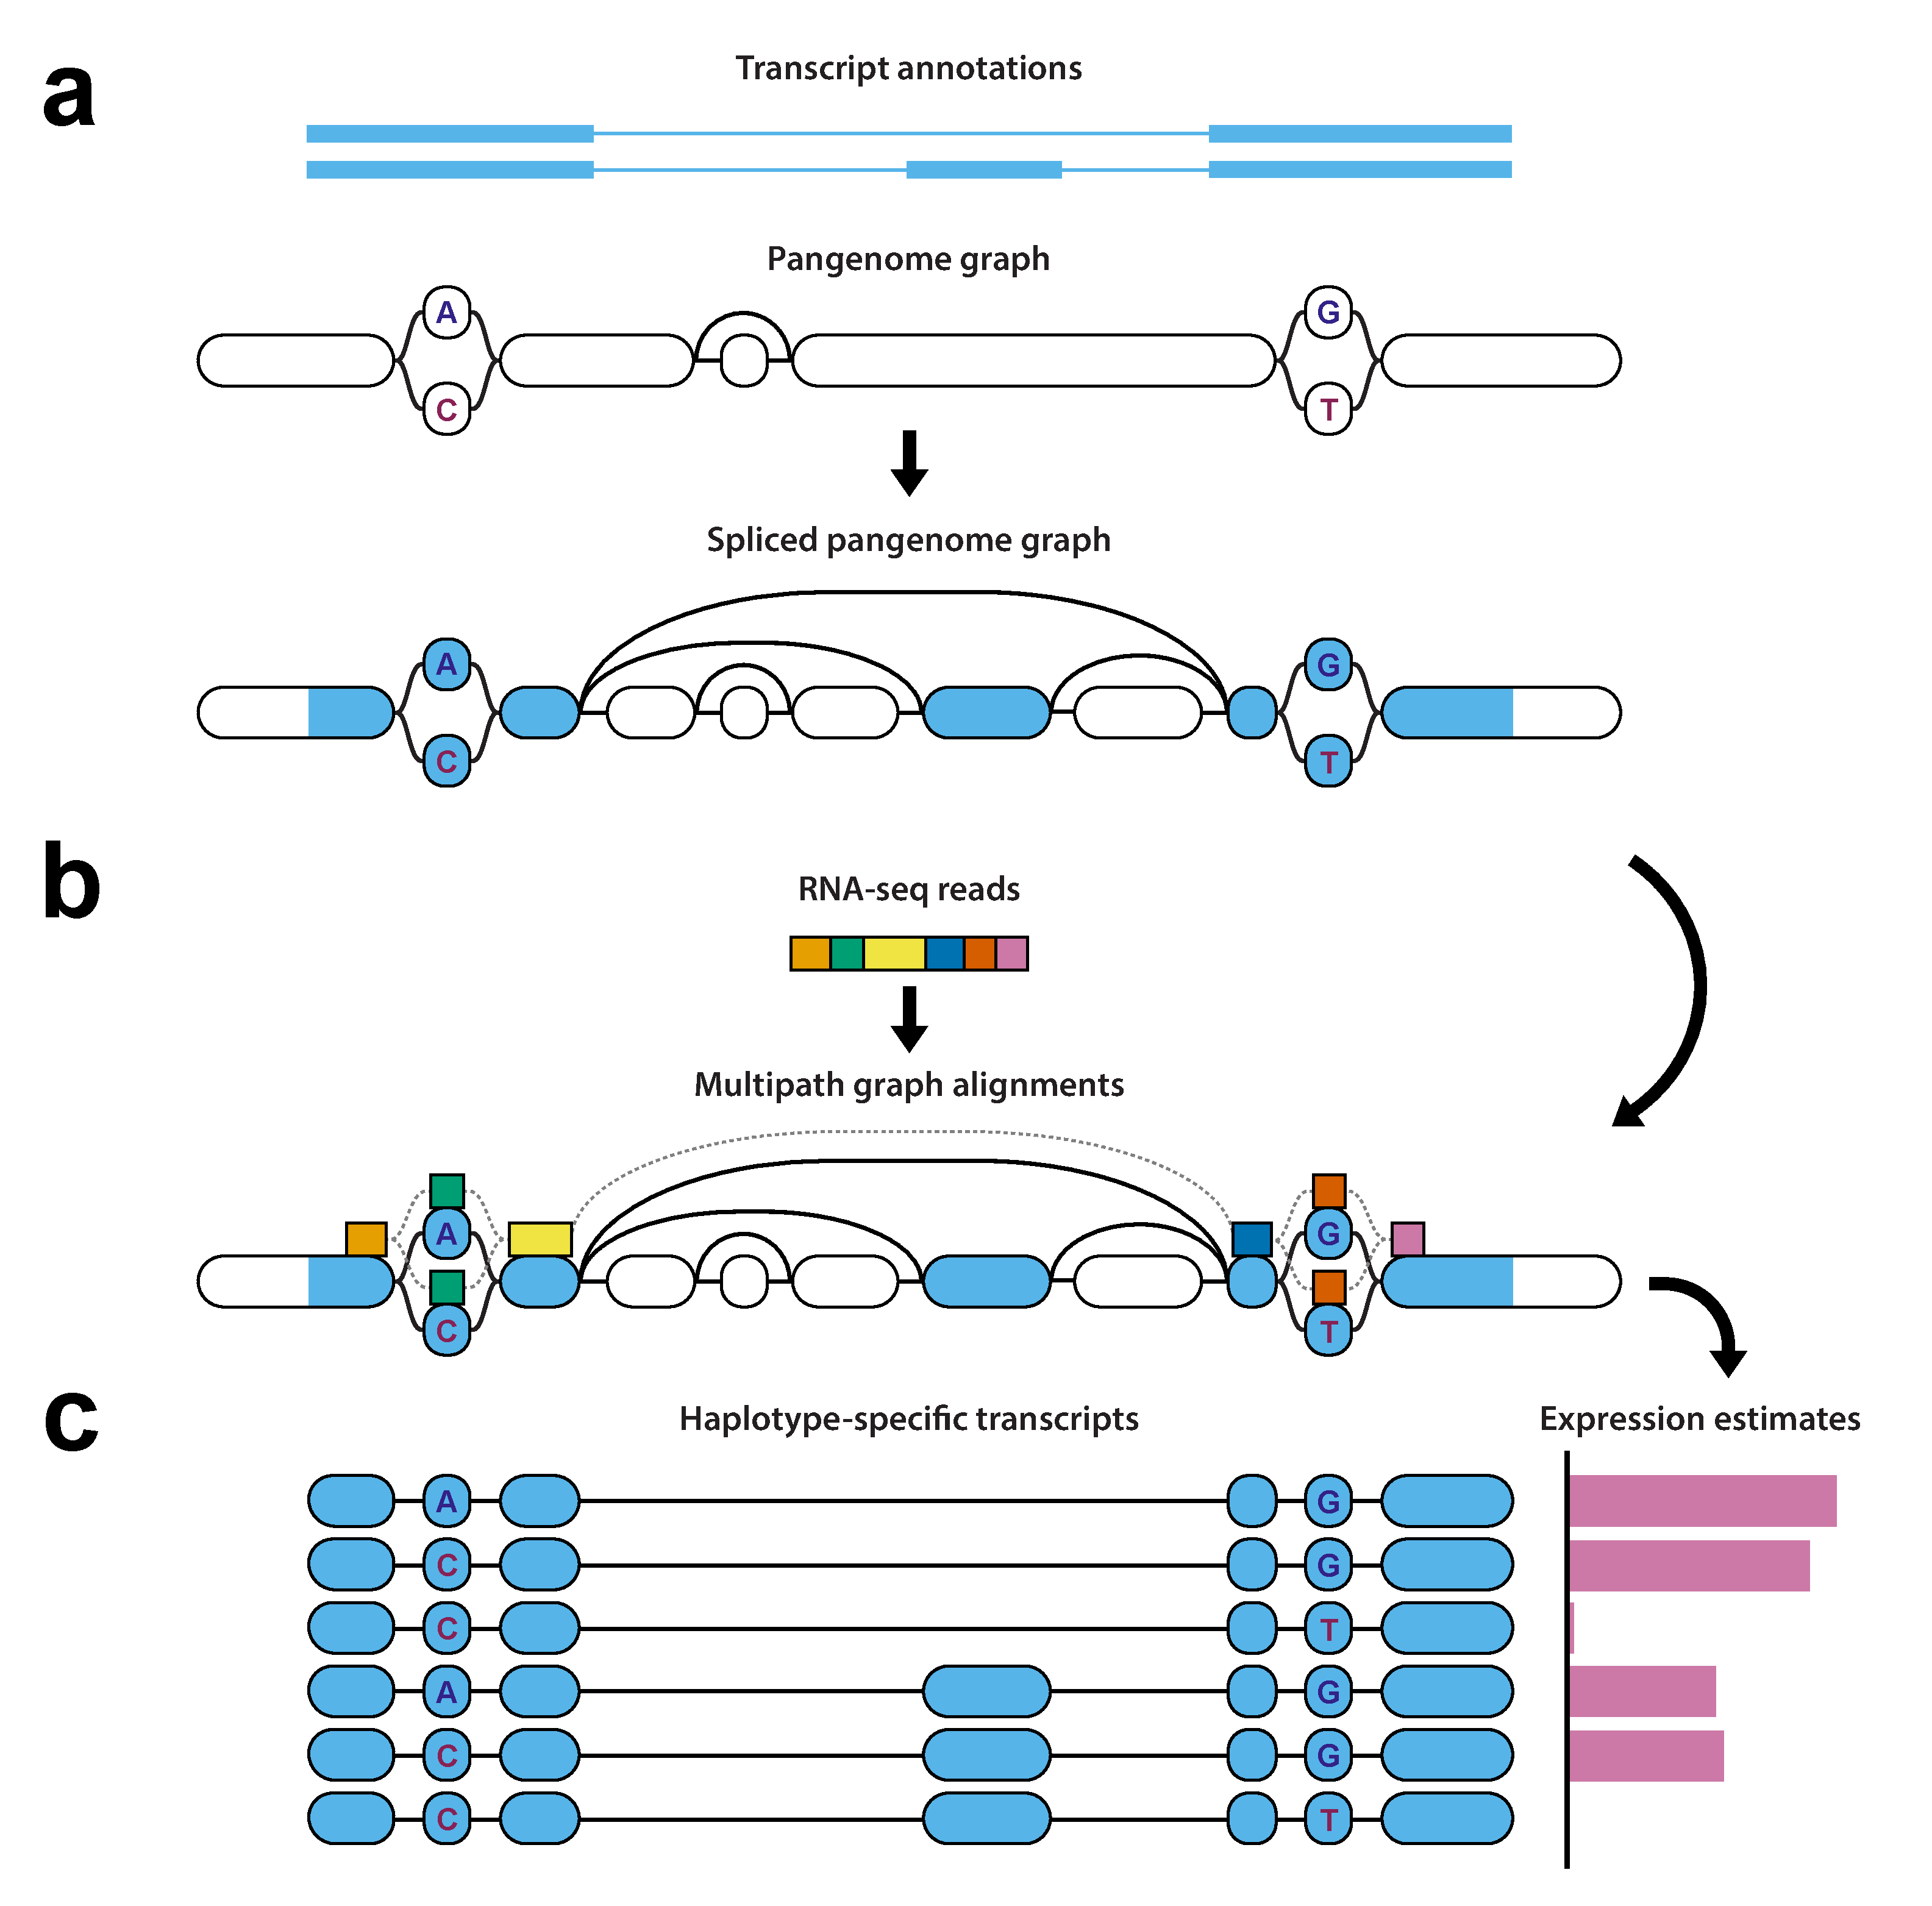
\includegraphics[width=.75\textwidth]{mpmapfigures/figure1.pdf}
\caption{\textbf{Diagram of haplotype-aware transcriptome analysis pipeline} \\
The three major steps in the pipeline. \textbf{a} \tool{vg rna} adds splice junctions derived from a transcript annotation to a pangenome graph to create a spliced pangenome graph. It simultaneously creates a pantranscriptome composed of a set of haplotype-specific transcripts (HSTs) using a panel of known haplotypes (not shown). \textbf{b} \tool{vg mpmap} aligns RNA-seq reads to subgraphs of the spliced pangenome graph represented as a multipath alignment. \textbf{c} \tool{rpvg} uses the alignments from \tool{mpmap} to estimate the expression of the HSTs in the pantranscriptome.
} \label{fig:overview}
\end{center}
\end{figure}

\subsection{Haplotype-aware transcriptome analysis pipeline}

In short, our pipeline works as follows (see Methods for a more detailed description). First, we construct a spliced pangenome graph using \tool{vg rna}, a method developed as part of the vg toolkit \cite{garrison2018variation}. \tool{vg rna} adds splice junctions from a transcript annotation into a pangenome graph as edges and then labels the paths in the graph that correspond to transcripts (Figure~\ref{fig:overview}a). Simultaneously, \tool{vg rna} constructs a set of haplotype-specific transcripts (HSTs) from the transcript annotation and a set of known haplotypes by projecting the transcript paths onto each haplotype. \tool{vg rna} uses the Graph Burrows-Wheeler Transform (GBWT) to efficiently store the HST paths allowing the pipeline to scale to a pantranscriptome with millions of transcript paths \cite{siren2020haplotype}. Next, RNA-seq reads are mapped to the spliced pangenome graph using \tool{vg mpmap}, a new splice-aware graph mapper in the vg toolkit that can align across both annotated and unannotated splice junctions (Figure~\ref{fig:overview}b). \tool{vg mpmap} produces multipath alignments that capture the local uncertainty of an alignment to different paths in the graph (Supplementary Figure~\ref{fig:multipath-alignment}). Lastly, the expression of the HSTs are inferred from the multipath alignments using \tool{rpvg} (Figure~\ref{fig:overview}c). \tool{rpvg} uses a nested inference scheme that first samples the most probable underlying haplotype combinations (e.g.\ diplotypes) and then infers the HST expression using expectation maximization conditioned on the sampled haplotypes.

\subsection{RNA-seq mapping benchmark}

We compared \tool{vg mpmap} against three other mappers: \tool{STAR} \cite{dobin2013star}, \tool{HISAT2} \cite{kim2019graph} and \tool{vg map} \cite{garrison2018variation}. \tool{STAR} and \tool{HISAT2} can both use splicing information to guide mapping, but of the two only \tool{HISAT2} is able to also utilize genomic variants. \tool{vg map} is not a splice-aware mapper, but it is still able to map to spliced pangenome graphs, which contain both splicing and genomic variation edges. 

We used two different references for the comparison: the standard reference genome with added splice junctions (spliced reference) and a spliced pangenome graph containing both splice junctions and variants (spliced pangenome graph). For \tool{STAR} only the spliced reference was used. 

\begin{figure}[h!]
\ssp
\begin{center}
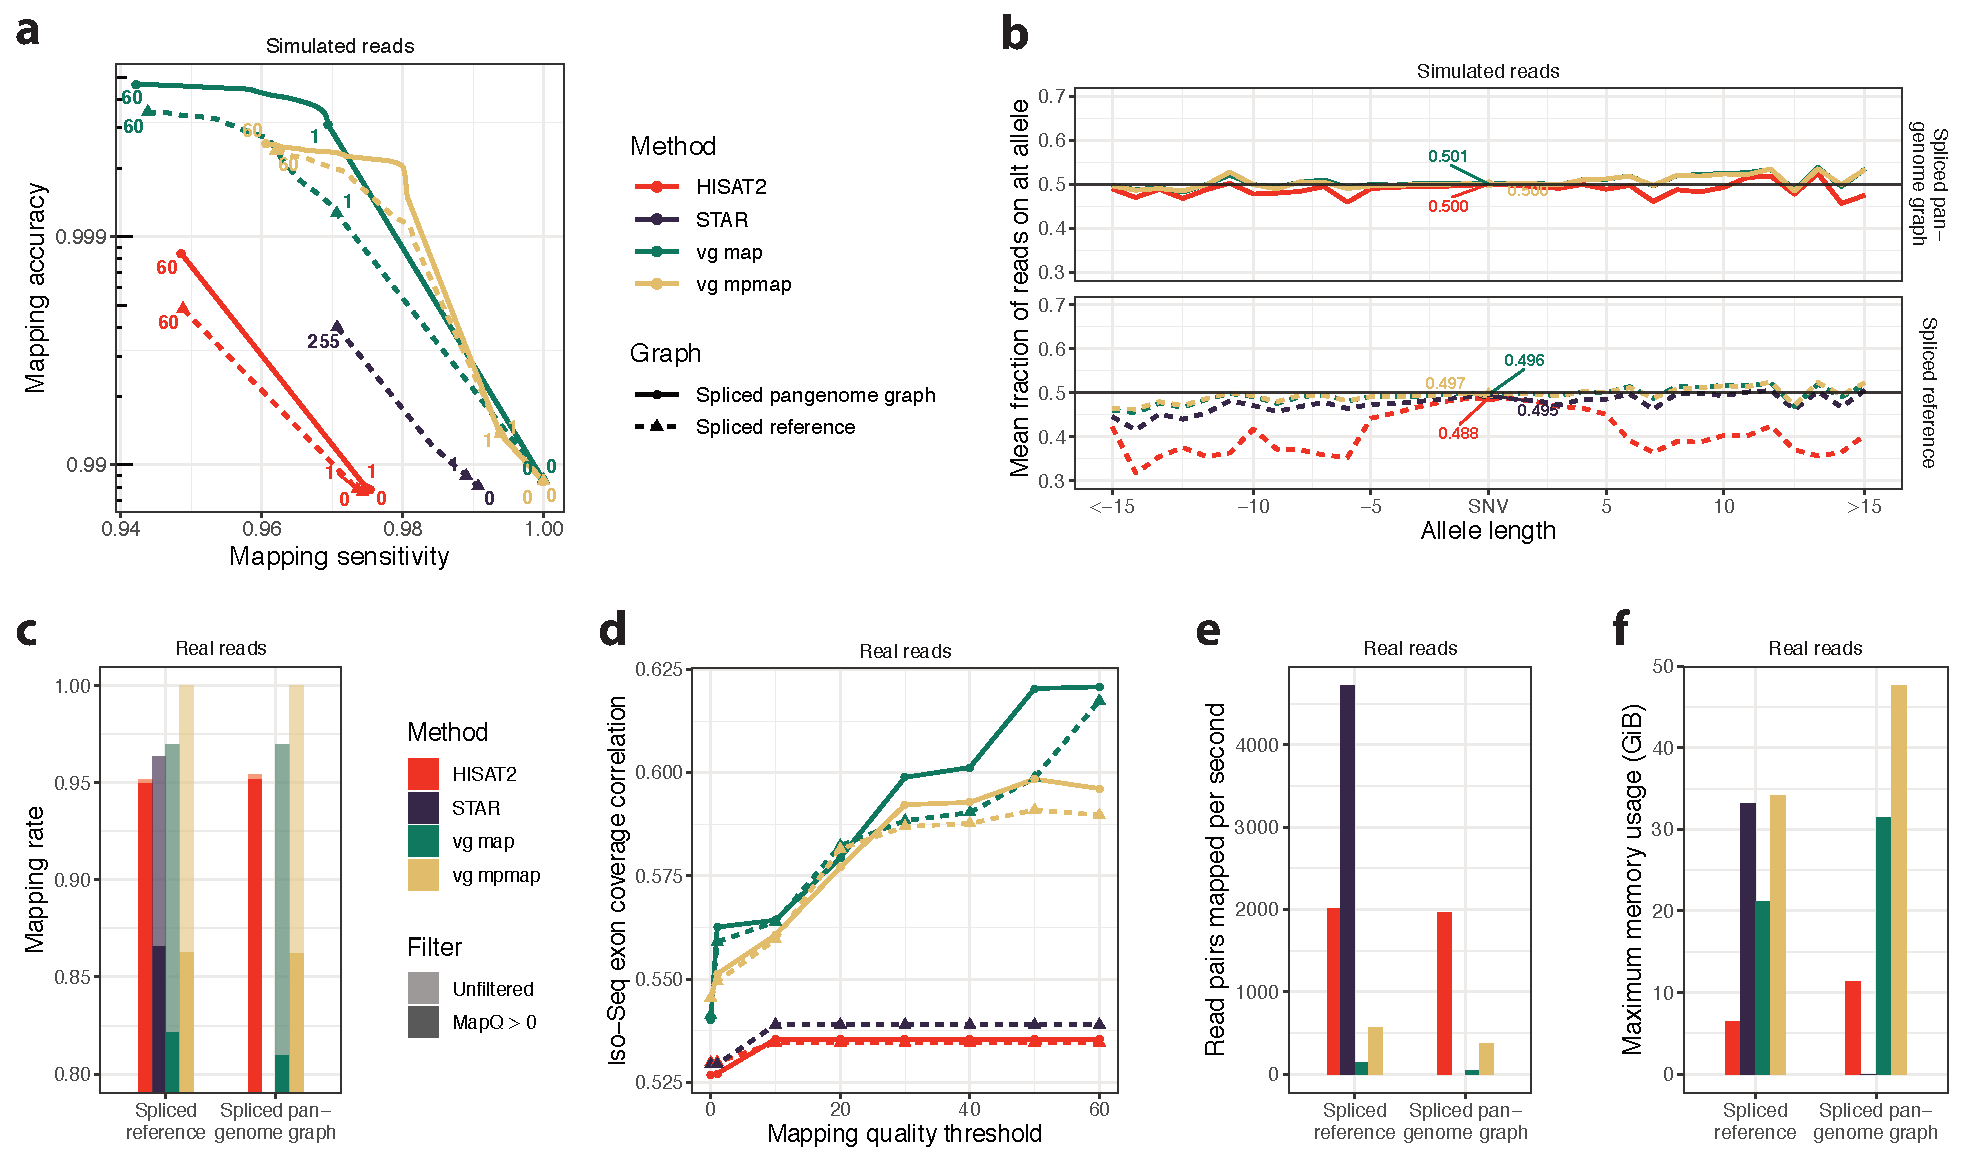
\includegraphics[width=\textwidth]{mpmapfigures/figure2.pdf}
\caption{\textbf{Mapping benchmark using RNA-seq data from NA12878} \\
RNA-seq mapping results comparing \tool{vg mpmap} and three other methods using simulated and real Illumina data (``vg sim (ENC, uniform)'' and ``ENCSR000AED'' in Supplementary Table~\ref{tab:sim-data} and~\ref{tab:read-sets}, respectively). Solid and dashed lines show the results using a spliced pangenome graph and spliced reference, respectively. \textbf{a} Mapping accuracy and sensitivity for different mapping quality thresholds (colored numbers) using simulated data. An alignment is considered correct if it covers 90\% of the true reference sequence alignment. \textbf{b} Mean fraction of mapped reads supporting the non-reference allele for variants of different lengths in simulated data. Negative lengths correspond to deletions and positive to insertions. The colored numbers are the mean fraction for SNVs. \textbf{c} Mapping rate using real data. The shaded bars show the mapping rate for all alignments and the solid bars for only alignments with a mapping quality above 0. \textbf{d} Pearson correlation between Illumina and Iso-Seq exon coverage using real data as a function of mapping quality threshold. Exons are defined by the Iso-Seq alignments. \textbf{e} Number of read pairs mapped per second per thread using real data. The mapping times were estimated using 16 threads on a AWS m5.4xlarge instance. \textbf{f} Maximum memory usage for mapping in gigabytes using real data.  
} \label{fig:mapping}
\end{center}
\end{figure}

\subsubsection{Simulated sequencing data}

Paired-end reads were simulated from HSTs derived from the GENCODE transcript annotation set \cite{frankish2019gencode} and the NA12878 haplotypes from the 1000 Genomes Project (1000GP) \cite{10002015global}. \tool{vg sim} was used to simulate the reads using reads from the ENCODE project (ENCSR000AED replicate 1) to parameterize the noise model \cite{encode2012integrated,davis2017encycolopedia}. Fragment length distribution parameters used in the simulation were estimated from the same reads using \tool{RSEM} \cite{li2011rsem}. The CEU population was excluded from the spliced pangenome graph as NA12878 is from that population, and we wanted to estimate performance for a new individual, who may not be as closely-related to the 1000GP populations. We simulated the HSTs with uniform expression rather than trying to match a previous expression profile, which could bias expression towards easily-mappable transcripts. 
\newline 
\newline 
Using the set of simulated reads we first compared the overall mapping performance of each method. Figure~\ref{fig:mapping}a shows the mapping sensitivity and accuracy (log-scale) for different mapping quality thresholds. An alignment was considered correct if it covered 90\% of the true reference sequence alignment. The graph alignments from \tool{vg map} and \tool{vg mpmap} were projected to the reference sequence for this comparison. As can be seen in Figure~\ref{fig:mapping}a, \tool{vg mpmap} achieves both a high sensitivity and accuracy, while the other methods either had a lower accuracy or sensitivity. The results also show that the spliced pangenome graph generally improves mapping performance. 

To evaluate the method's ability to align over unannotated splice junctions, we repeated the experiment on a spliced pangenome graph (spliced reference for \tool{STAR}) created from an annotation set with 20\% of the transcripts missing (Supplementary Figure~\ref{fig:splice-junction-mapping}). This number was based on recent estimates of the fraction of novel transcripts in a sample using long reads \cite{wyman2019technology}. As expected, the performance of \tool{vg map} decreases dramatically since it can only align over splice junctions represented in the graph. \tool{vg mpmap}'s performance decreased markedly more on the downsampled annotation compared to \tool{STAR} and \tool{HISAT2} using the 90\% threshold (Supplementary Figure~\ref{fig:splice-junction-mapping}a). This is likely due to its more conservative approach to finding novel splice-junctions that require a high-scoring alignment in order for a new junction to be statistically significant. Indeed, when using a threshold of 70\%, the mapping accuracy \tool{vg mpmap} increases to a value higher than \tool{STAR} and \tool{HISAT2} even when they use the complete transcript set (Supplementary Figure~\ref{fig:splice-junction-mapping}b).

Next, we looked at whether using a variant-aware approach reduces reference bias. Figure~\ref{fig:mapping}b shows the mean fraction of reads mapped to the alternative allele for different allele lengths. Negative values correspond to deletions and positive values to insertions. When using the spliced reference genome, all methods exhibit a bias towards the reference allele, with \tool{vg map} and \tool{mpmap} showing less bias than the other methods. Using the spliced pangenome graph results in substantially reduced bias for all 
methods.

The mapping results were corroborated by an alternate correctness criterion based on aligning within 100 bases of the correct position on the paths in the graph (Supplementary Figure~\ref{fig:mapping-gampcompare}).
\newline 
\newline
The set of simulated reads used for the mapping evaluation was not used to optimize the development and parameters of \tool{vg map} and \tool{mpmap}. Supplementary Figure~\ref{fig:mapping-srr}a shows the results on the dataset that was used for optimization, which used RNA-seq data from Tilgner et al. \cite{tilgner2014defining} to parameterize the read simulation. The sensitivity and accuracy estimates for \tool{mpmap} are quite similar between the two datasets indicating that \tool{mpmap} is not overfit to the training data. The performance of all the other methods was generally worse on the training data. 

\subsubsection{Real sequencing data}

We used the same read set from the ENCODE project that was used to parametrize the simulations to benchmark the methods on real data. We first looked at the fraction of aligned reads for each method (Figure~\ref{fig:mapping}c). \tool{vg mpmap} was able to map more reads overall than any of the other methods. \tool{HISAT2} achieved a higher mapping rate for mappings with mapping quality greater than 0, but seemingly at the cost of low specificity (Figure~\ref{fig:mapping}a). Using the spliced pangenome graph did not have a notable influence on the mapping rates. 

Ground-truth alignments are not available for real data, so we use a proxy based on Pacific Biosciences (PacBio) Iso-Seq read mappings instead. Specifically, we compare to Iso-Seq read alignments generated by the ENCODE project (ENCSR706ANY) from the same cell line as the Illumina reads. Since the cell line is the same, we expect the transcript expression to be similar. Moreover, long reads can generally be mapped more confidently than short reads. Thus, higher correlation in coverage between short read mappings and the Iso-Seq mappings should be indicative of more accurate short read mappings in the aggregate. Figure~\ref{fig:mapping}d shows the estimated Pearson correlation in the coverage of each exon as a function of mapping quality threshold. As can be seen, both \tool{vg map} and \tool{mpmap} achieves higher correlation than \tool{STAR} and \tool{HISAT2}, with the spliced pangenome graph resulting in even higher correlation for both. The graph alignments from \tool{vg map} and \tool{mpmap} were projected to the reference genome for this analysis.  

Finally, we compared the methods' mapping speed and memory usage. Figure~\ref{fig:mapping}e shows the number of read pairs mapped per second per thread. Conversion from SAM to BAM was included in the \tool{HISAT2} time estimate to be more comparable to the output type of the other methods. \tool{vg mpmap}'s increase in accuracy does not come for free; it is between 3.6 and 5.2 times slower than \tool{HISAT2}, depending on the graph. However, it is 9.4 times faster than \tool{vg map} on the spliced pangenome graph. \tool{vg mpmap} uses slightly more memory than \tool{STAR} (Figure~\ref{fig:mapping}f). 
\newline 
\newline
We also compared the mapping performance of the different methods on the real RNA-seq data from Tilgner et al. \cite{tilgner2014defining} and CHM13 RNA-seq data from the T2T consortium (Supplementary Figure~\ref{fig:mapping-srr}b,c and~\ref{fig:mapping-t2t}). Similar overall tendencies are observed using these datasets. It is important to mention that the CHM13 data was used during the development of \tool{vg mpmap}, and the other set was used to optimize the parameters of \tool{vg map} and \tool{vg mpmap}.

\subsection{Haplotype-specific transcript quantification}

\begin{figure}[h!]
\ssp
\begin{center}
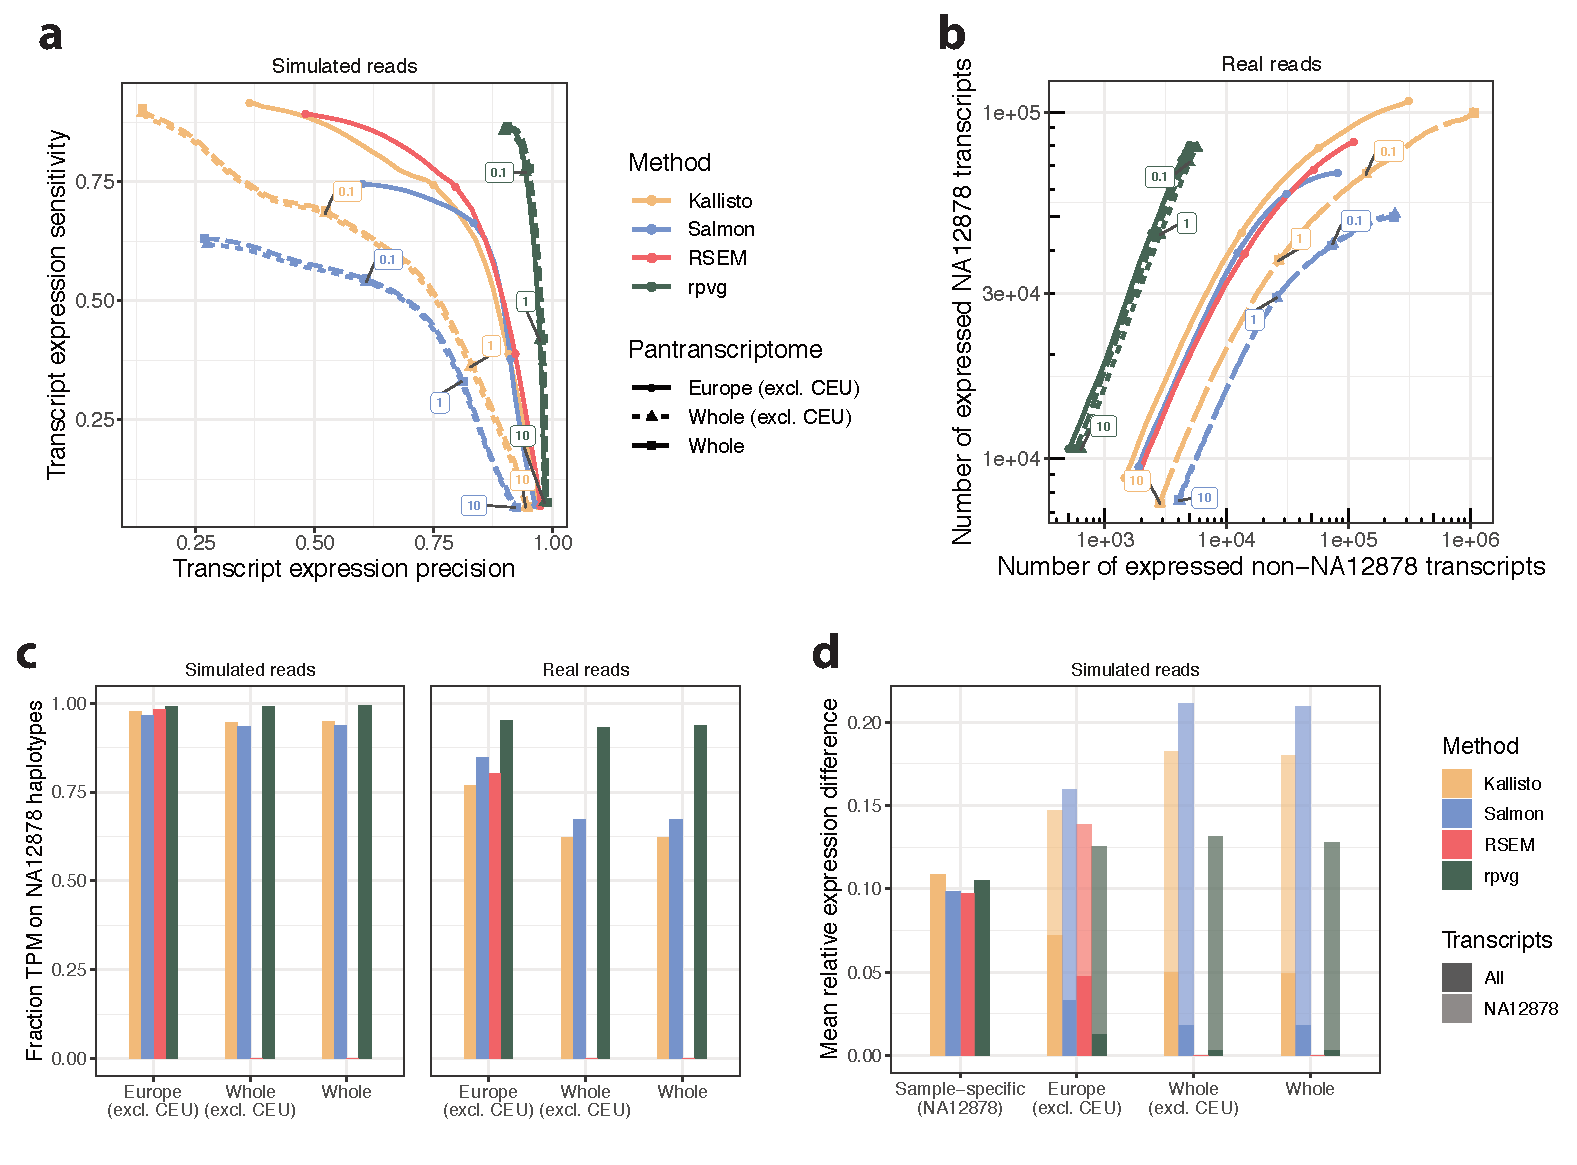
\includegraphics[width=.85\textwidth]{mpmapfigures/figure3.pdf}
\caption{\textbf{Haplotype-specific transcript quantification benchmark using RNA-seq data from NA12878} \\
Haplotype-specific transcript (HST) quantification results comparing \tool{rpvg} against three other methods using simulated and real Illumina data (``vg sim (ENC, RSEM)'' and ``ENCSR000AED'' in Supplementary Table~\ref{tab:sim-data} and~\ref{tab:read-sets}, respectively). Solid lines with circles are results using a pantranscriptome generated from 1000 Genomes Project (1000GP) European haplotypes excluding the CEU population. Dashed lines with triangles and squares are results using a pantranscriptome generated from all 1000GP haplotypes without and with the CEU population, respectively. \textbf{a} Sensitivity and precision of whether a transcript is correctly assigned nonzero expression for different expression value thresholds (colored numbers for ``Whole (excl. CEU)'' pantranscriptome) using simulated data. Expression is measured in transcripts per million (TPM). \textbf{b} Number of expressed transcripts from NA12878 haplotypes shown against the number from non-NA12878 haplotypes for different expression value thresholds (colored numbers) using real data. \textbf{c} Fraction of transcript expression (in TPM) assigned to NA12878 haplotypes for different pantranscriptomes using simulated (left) and real (right) data. \textbf{d} Mean absolute relative difference (MARD) between simulated and estimated expression (in TPM) for different pantranscriptomes using simulated data. MARD was calculated using either all HSTs in the pantranscriptome (solid bars) or using only the NA12878 HSTs (shaded bars). ``Sample-specific (NA12878)'' is a personal transcriptome generated from 1000GP NA12878 haplotypes.  
} \label{fig:expression}
\end{center}
\end{figure}

We compared \tool{rpvg} to three other transcript quantification methods: \tool{Kallisto} \cite{bray2016near}, \tool{Salmon} \cite{patro2017salmon} and \tool{RSEM} \cite{li2011rsem}. We stress that none of these methods were developed to work on pantranscriptomes with millions of HSTs. However, they serve as a point of reference for what accuracy is achievable without new methods development. The simulated data was generated by \tool{vg sim}, largely as described for the mapping benchmark. The only difference was that, rather than simulating transcripts with uniform expression, we simulated according to an expression profile that was estimated by \tool{RSEM} using the same ENCODE reads. Three different pantranscriptomes were generated for the evaluation using different sets of 1000GP haplotypes (Supplementary Table~\ref{tab:pantranscriptomes}): 1) all European haplotypes excluding the CEU population (Europe (excl. CEU)) 2) all haplotypes excluding the CEU population (Whole (excl. CEU)) and 3) all haplotypes (Whole). The CEU population was excluded for the same reason as in the mapping benchmark: because NA12878 is part of this population, and we wanted to evaluate the realistic setting in which a sample is not as well represented by the haplotype panel. In addition, we created a sample-specific transcriptome consisting of NA12878 HSTs (Sample-specific (NA12878)). This transcriptome corresponds to the ideal case where a sample's haplotypes are known beforehand. 
\newline 
\newline
We first looked at the method's ability to accurately predict whether an HST was correctly expressed or not. Figure~\ref{fig:expression}a shows the sensitivity and precision of whether a transcript is correctly expressed or not using simulated data. The results were stratified by different expression thresholds up to a value of 10 TPM (transcripts per million). Note that we were not able to run \tool{RSEM} on the two largest pan-transcriptomes used in the figure. \tool{rpvg} exhibits a mucher higher precision and sensitivity than the other tools for all pantranscriptomes. Over 97.4\% of the HSTs with an expression value of at least 1 TPM are correctly predicted to be expressed by \tool{rpvg} using the ``Whole (excl. CEU)'' pantranscriptome. Importantly, only a minor difference is observed between the pantranscriptomes without the CEU population (excl. CEU) and the whole pantranscriptome (Whole), which contains NA12878. This could be explained by the fact that less than 2\% of HSTs are on average unique to a specific sample when compared to all samples in other populations using the 1000GP data (Supplementary Figure~\ref{fig:hst-populations}). This suggests that haplotype panels like the 1000GP are a good alternative when a sample's haplotypes are not available, although there are always limits to panel diversity, and some samples will be less well-represented by a 1000GP pantranscriptome. 

We also evaluated the accuracy of the HST expression estimation using real sequencing data (Figure~\ref{fig:expression}b). Since we do not know which transcripts are expressed in real data, we focus instead on the haplotype estimation. Sample NA12878's haplotypes are known to a reasonably high degree of certainty. Thus, we can indirectly measure accuracy by asking whether the HSTs that are estimated to be expressed are in fact from NA12878. Similar to the simulated data, Figure~\ref{fig:expression}b shows that \tool{rpvg} predicts markedly fewer HSTs from non-NA12878 haplotypes than both \tool{Kallisto} and \tool{Salmon}. Using the ``Whole (excl. CEU)'' pantranscriptome, \tool{rpvg} predicted 2,836 HSTs from non-NA12878 haplotypes to have an expression value of at least 1 TPM, while \tool{Salmon} and \tool{Kallisto} predicted 25,790 and 26,779, respectively. 

Next, we compared the fraction of transcript expression (in TPM) that was attributed to NA12878 haplotypes. This is shown in Figure~\ref{fig:expression}c for both simulated (left bars) and real (right bars) data. We see that \tool{rpvg} attributes more than 98.9\% and 93.1\% of the expression to NA12878 haplotypes when using simulated and real data, respectively. Furthermore, the figure shows that \tool{rpvg}'s prediction accuracy only decreases slightly when the size of the pantranscriptome increases from 2.5M HSTs in ``Europe (excl. CEU)'' to 11.6M in ``Whole (excl. CEU)''.  
\newline 
\newline
We compared how well the different methods could predict the correct expression value. Figure~\ref{fig:expression}d shows the mean absolute relative difference (MARD) between the expression values of the simulated reads and the estimated values. The solid bars are MARD values when using all HSTs in the pantranscriptomes, and the shaded bars are when comparing the NA12878 HSTs only. Note that these bars are the same for the sample-specific set, which consists of only NA12878's HSTs. On the sample-specific set, \tool{rpvg} performs comparably to the other methods. However, as the size of the pantranscriptome grows, the increase in MARD on the NA12878 transcript set is considerably less for \tool{rpvg} relative to the other methods. When looking at the whole transcript set in each pantranscriptome (solid bars), \tool{rpvg} has the lowest MARD. The much lower values compared to the NA12878 transcript set can be explained by the large number of unexpressed HSTs in the full pantranscriptomes.

We also compared the expression values using Spearman correlation (Supplementary Figure~\ref{fig:expression-corr}). This metric supported overall similar conclusions, albeit with \tool{Kallisto} and \tool{RSEM} performing comparably to \tool{rpvg} when using the pantranscriptomes but restricting focus to NA12878's haplotypes. This suggests that \tool{Kallisto} and \tool{RSEM} accurately rank these transcripts' expression but do not accurately estimate the absolute quantity.
\newline 
\newline
To show the advantage of the multipath alignment format when inferring HST expression we repeated the evaluation using single-path alignments as input to \tool{rpvg} (Supplementary Figure~\ref{fig:expression-multipath}). The single-path alignments were created by finding the best scoring path in each multipath alignment. For all pantranscriptomes and datasets, \tool{rpvg} gave the best results using the multipath alignments.

Similarly to the mapping benchmark, we also evaluated \tool{rpvg} on RNA-seq data from the CHM13 cell line and NA12878 RNA-seq data from Tilgner et al. \cite{tilgner2014defining} (Supplementary Figure~\ref{fig:expression-t2t} and~\ref{fig:expression-srr}). Overall, similar conclusions can be drawn using these data. It is important to mention that both datasets were used to optimize the parameters of \tool{rpvg}.

\subsection{Assaying isoform-specific genomic imprinting}

\begin{figure}[h]
\ssp
\begin{center}
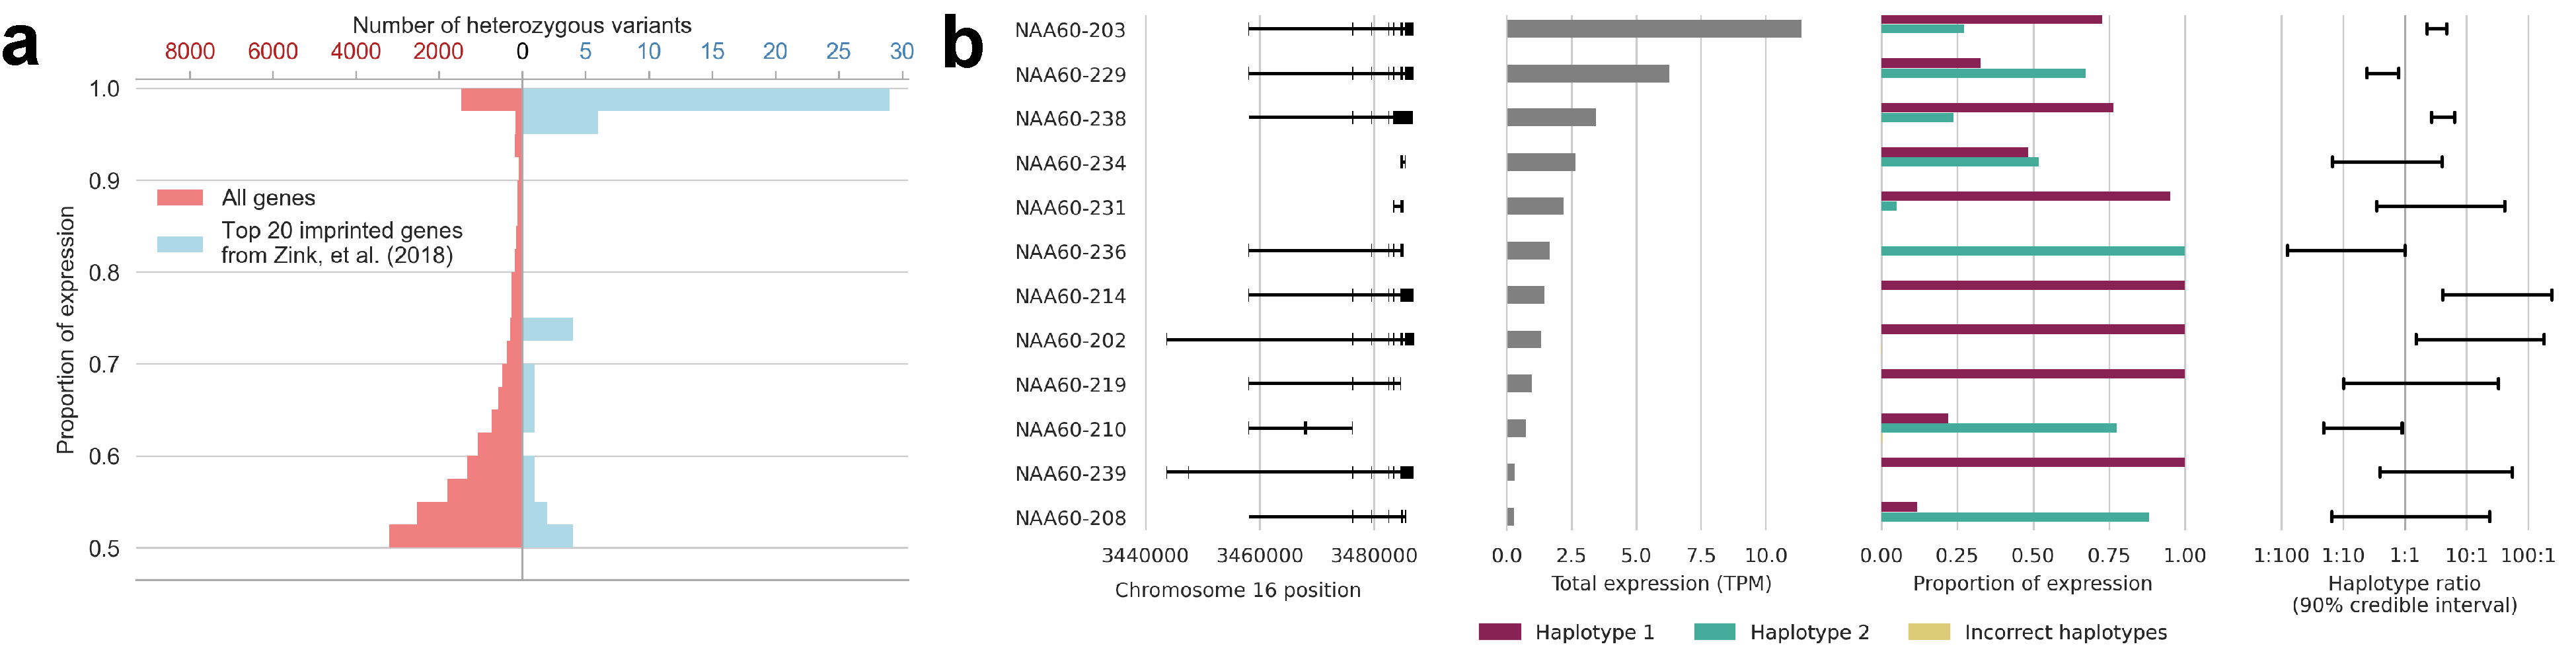
\includegraphics[width=\textwidth]{mpmapfigures/figure4.pdf}
\caption{\textbf{Exploratory demonstration of analyzing genomic imprinting using data from GM12878 lymphoblastoid cell line} \\
Results of the \tool{vg mpmap}-\tool{rpvg} pipeline on RNA-seq data from a lymphoblastoid cell line from the ENCODE Project, focusing on genes previously identified as imprinted in blood. \textbf{a} The proportion of expression attributed to the higher-expressed allele of heterozygous variants among the 20 most significantly imprinted genes from Zink's, et al. study \cite{zink2018insights} compared to all genes. The axes are scaled so that both histograms have the same area. \textbf{b} Isoform-level allele specific expression in NAA60, which was previously identified as imprinted but not as having isoform-dependent reversals in the polarity of imprinting\cite{zink2018insights}. Isoforms with expression less than 0.25 transcripts per million (TPM) are not shown.
} \label{fig:imprinting}
\end{center}
\end{figure}

To demonstrate the utility of the \tool{vg mpmap}-\tool{rpvg} pipeline, we performed an exploratory analysis of genomic imprinting in a human sample. Genomic imprinting is the phenomenon in mammals in which some genes are expressed only from the copy inherited from a specific parent. That is, either the maternal or paternal copy is silenced, regardless of the genomic sequence of that haplotype. This is accomplished through mitotically heritable epigenetic modifications that are established during early development\cite{tucci2019genomic}.

Several previous studies have studied imprinting genome-wide by quantifying ASE in RNA-seq data. These studies have demonstrated that imprinting varies substantially across tissues \cite{baran2015landscape,babak2015genetic} and varies in intensity across genes, with many genes showing biased expression away from one parent-of-origin copy but not complete silencing\cite{babak2015genetic,jadhav2019rna,zink2018insights}. In addition, a handful of genes have been identified in which the polarity of imprinting depends on the isoform: some isoforms of the same gene are biased toward the paternal copy and others toward the maternal copy\cite{zink2018insights}.

The previous genome-wide studies have methodological limitations that diminish their ability to detect isoform-level imprinting. Some have aggregated ASE across all isoforms of the gene, which precludes isoform-level analysis a priori\cite{baran2015landscape,babak2015genetic,jadhav2019rna}. The largest study, by Zink, et al. \cite{zink2018insights}, performed all tests of imprinting on individual SNVs. This method can sometimes detect isoform-level differences if the isoforms have some unshared exons. However, in shared exons, the ASE signal from the highest-expressed isoforms can drown out the signal of lower-expressed isoforms. Depending on the configuration of exons in the isoforms, this can make it very challenging to identify imprinting of opposite polarity within the same gene.

Figure \ref{fig:imprinting} shows results from our exploratory demonstration of isoform-level imprinting analysis using \tool{vg mpmap} and \tool{rpvg}. We ran the entire pipeline using RNA-seq data from a lymphoblastoid cell line derived from 1000 Genomes Project sample NA12889, which was sequenced as part of the Geuvadis project\cite{lappalainen2013transcriptome}. As a confirmatory analysis, we first looked for ASE in genes that have previously been identified as imprinted. In particular, we looked at the 20 genes with the most significant $p$-values from Zink's, et al. study\cite{zink2018insights}. To mirror the methods used in this paper, we derived variant-specific ASE values by aggregating the expression across all HSTs that contain a given allele for a variant. Figure \ref{fig:imprinting}a shows that the \tool{vg mpmap}-\tool{rpvg} pipeline detects ASE at heterozygous variants in these imprinted genes at a markedly higher rate than in background across all genes.

The \tool{vg mpmap}-\tool{rpvg} pipeline is also capable of detecting isoform-dependent genomic imprinting. Figure \ref{fig:imprinting}b shows an illustrative example in the gene NAA60, which codes for an enzyme that acetylates the N-terminus of proteins in the Golgi apparatus. The isoforms show a complex pattern of imprinting polarity, which does not correlate strongly with exons or start sites in any particular genomic region. Given the large differences in expression of these isoforms, the SNV-based analysis would have had difficulty identifying imprinting in the more lowly-expressed isoforms, and indeed this gene was reported as imprinted (in fact, it is among the 20 most significantly genes referred to above) but not as having isoform-dependent imprinting\cite{zink2018insights}. It should be emphasized that this exploratory analysis of a single sample, while suggestive, is insufficient to conclusively demonstrate isoform-dependent imprinting in NAA60. Doing so would require further biological replicates and more rigorous controls for cis-regulation and cell line clonality\cite{jadhav2019rna}.

\section{Discussion}

The pace of development in the field of eukaryotic pangenomics has surged in recent years. Improvements in sequencing technology have made it practical to characterize the genomes of increasingly many samples. As a result, pangenomes made from tens to hundreds of reference-quality genome assemblies have been constructed for several agricultural organisms \cite{jayakodi2020barley,crysnanto2019accurate,liu2020pan}, and similar efforts are underway for humans by the Human Pangenome Reference Consortium and others \cite{ebert2021haplotype}. Simultaneously, the bioinformatics tools to do pangenomic analyses have matured to the point of practicality for many applications \cite{manuweera2019pangenome,hickey2020genotyping,siren2020genotyping}. Moving forward, we anticipate that pangenomic methods will continue to expand to inform increasingly many areas of genomics \cite{groza2020personalized}.

In this work, we have presented one step in this expansion: generalizing transcriptomics into pantranscriptomics. Our novel bioinformatics pipeline provides a full stack of tools for pantranscriptomic analysis. It can construct pantranscriptomes, map RNA-seq reads to these pantranscriptomes, and quantify transcription with haplotype-resolution. The construction takes advantage of efficient pangenome data structures, the mapping achieves a desirable balance of accuracy and speed, and the quantification can infer haplotype-specific transcript expression even when the sample's haplotypes are not known beforehand.

Some downstream applications are already apparent. For one, the pipeline can be used to study causes of haplotype-specific differential expression. We demonstrated its capabilities on one such example: genomic imprinting. The demonstration showed suggestive evidence of complex patterns of imprinting at the isoform level, which would have difficult or impossible to detect with previous genome-wide methodologies. The pipeline could be similarly used to study other sources of haplotype-specific expression, such as nonsense-mediated decay and cis-regulation. 

Another application is characterizing genotypes and haplotypes in coding regions from RNA-seq data. This could give access to the exact transcript sequences in a sample's transcriptome. In both of these applications, this pipeline increases the information that is available from RNA-seq data without paired genomic sequencing. This will enable low-cost study designs and deeper reanalyses of existing data.

Of course, our pipeline also has limitations. We have developed it to have good performance on pantranscriptomes constructed from phased variant calls. This is presently the most available data resource for constructing pangenomes. However, as increasingly many haplotype-resolved assemblies are produced, we predict that the emphasis in pangenomics will shift to pangenome graphs constructed from whole genome alignments. Constructing these graphs is currently an area of active research \cite{li2020design,jandrasits2018seq}. Such graphs have more complicated topologies, often involving complex cyclic motifs. Experience leads us to believe that pantranscriptomic tools will require further methods development to use these data resources effectively.

Our pipeline is optimized for short-read RNA-seq data. The higher-error long-read RNA-seq technologies developed more recently require specifically-tailored algorithms for efficient analysis \cite{li2018minimap2,wyman2019technology}. Pantranscriptomic analyses of long-read RNA-seq data will likewise require further development, although the pipeline described here could serve as a platform for this development. Nevertheless, the cost-effectiveness of short-read sequencing virtually ensures that it will remain an important part of the sequencing landscape into the near future.
Finally, our pipeline also relies on having a comprehensive pantranscriptome that contains many of the sample's haplotype-specific transcripts. The pantranscriptomes used in this study (based on the 1000 Genome Project) provided good results in the three samples analyzed, but this performance may not extend to samples from other populations. Here---and throughout pangenomics---there is a compelling case to improve the completeness of data resources through more diverse sampling.

%%%%%%%%%%% Comment thread imported from Google doc %%%%%%%%%%%%%%%
% Benedict: Might also be worth mentioning single-cell applications. e.g. Imagine trying to quantify somatic haplotype-specific expression in subsets of tumor cells? I appreciate this is a bit science fiction now, but perhaps not for too much longer.
% Jordan: I don't think I totally understand this use case, tbh. What's the edge we get from bringing a pantranscriptomic methodology?
% Benedict: sorry, totally half baked, but what I was thinking vaguely was that if you could build tumor-specific transcripts from dna sequencing of a tumor you could use the approach to quantify tumor-haplotype specific expression? again, half baked.
% Jordan: Hmm. We could probably do that analysis with mpmap/rpvg, but it seems to me the harder part would be the DNA sequencing. You'd need to produce something like a phased "tumor pangenome", and you'd have to do the phasing without even the benefit of assuming unbiased coverage of 2 haplotypes (because the fraction of clonal populations differs).
% Jonas: One thing we could try is to use mpmap/rpvg to infer the germline haplotypes and quantify the expression of germline haplotype-specific transcripts in a cancer RNA-seq sample. This could maybe then be used as a "background" for downstream somatic variant/expression analyses (haven't thought this through thoroughly yet). I think this might be doable with the pipeline already assuming that somatic variation are different from the variants in the pantranscriptome (which I think is a fair assumption). I have no idea how mpmap/\tool{rpvg} will perform on this data, but it could be interesting to explore this maybe as part of the use-case figure.
% Jordan: I think that's reasonable but also comfortably fits under the umbrella of the "low cost study designs and deeper reanalyses" that we already mention, since the mpmap/\tool{rpvg} portion would basically just be treating the scRNA-seq as bulk sequencing. Is the goal here just to mention a single cell application? If so, I think it would be less of a stretch to focus on random mono-allelic expression in somatic tissues. That's an analysis that we would actually need single cell sequencing for.

\section{Acknowledgements}

Research reported in this publication was supported by the National Human Genome Research Institute of the National Institutes of Health under Award Numbers U01HG010961 and R01HG010485. The content is solely the responsibility of the authors and does not necessarily represent the official views of the National Institutes of Health. The work of JAS was supported by the Carlsberg Foundation. We thank the ENCODE Consortium, the Thomas Gingeras Laboratory (Cold Spring Harbor Laboratory) and the Ali Mortazavi Laboratory (University of California Irvine) for generating and sharing the ENCODE data used in this study. We would also like to thank Megan Dennis (University of California Davis) for generating and providing access to the CHM13 RNA-seq data on behalf of the T2T consortium. Finally, we would like to thank Jean Monlong and Glenn Hickey for feedback on the manuscript, and everybody else in the vg team.

\section{Methods}

\subsection{Sequencing data, transcript annotations and variation databases}

GENCODE v29 (primary assembly) was used as a transcript annotation set \cite{frankish2019gencode}. All transcripts with either the mRNA\_start\_NF or mRNA\_end\_NF tag were removed in order to only keep confirmed full-length transcripts. Furthermore, a transcript subset containing 80\% of the GENCODE transcripts was created by randomly removing 34,490 of the 172,449 transcripts in the annotation. The fraction removed was based on recent estimates of the fraction of novel transcripts in a sample using long reads \cite{wyman2019technology}.

Genomic variants on GRCh38 from the 1000 Genomes Project (1000GP) were downloaded from EBI (\url{http://ftp.1000genomes.ebi.ac.uk/vol1/ftp/release/20130502/supporting/GRCh38_positions/}) \cite{10002015global}. The variants were first normalized using \tool{bcftools} \cite{Li2011-xc} and four different sets containing variants from differently-sized collections  of samples were created (Supplementary Table~\ref{tab:haplotype-sets}). Two of these sets were constructed so as to not include variants unique to the CEU population. This was because we benchmarked the pipeline on NA12878, who is from this population, and we wanted our evaluations to cover one of the intended use-cases for the pipeline: sequencing a new sample from a population that is not represented in the reference haplotype panel. For all of the variant sets except the sample-specific set (where allele frequency was not relevant), the intronic and intergenic variants were further filtered using \tool{bcftools}, keeping only variants with an alternative allele frequency of at least 0.002 or 0.001 depending on the set. This was done to decrease the complexity of the graph in regions where fewer reads are expected to map. The GRCh38 (primary assembly) reference genome used throughout the study was downloaded from Ensembl (\url{ftp://ftp.ensembl.org/pub/release-94/fasta/homo_sapiens/dna/}).  
\newline 
\newline
A list of all sequencing data used can be found in Supplementary Table~\ref{tab:read-sets}. 

\subsection{Spliced pangenome graph construction}

We developed a method in the vg toolkit, \tool{vg rna}, for constructing spliced pangenome graphs from a transcript annotation and an existing pangenome graph. \tool{vg rna} begins by identifying the path in the graph that corresponds to each exon in the annotation. This process is facilitated by indexes in the vg toolkit that can efficiently query graph locations of positions on the linear reference. These exon paths can start or end internally in a node rather than only at boundaries between nodes, as with other paths in vg. Next, \tool{vg rna} divides nodes as necessary to expose exon boundaries as node boundaries and then adds edges (splice-junctions) to the graph connecting adjacent exons within each transcript. The transcript paths are then labeled in the resulting spliced pangenome graph. Lastly, the spliced pangenome graph's node ID space is compacted and reordered in topological order to make graph compression more efficient \cite{eizenga2020efficient}. 
\newline 
\newline
In addition to the spliced pangenome graphs, \tool{vg rna} was also used to construct exon-only splicing graphs. \tool{vg rna} creates these graphs by removing all nodes and edges from a spliced pangenome graph that were not covered by a transcript path. Different combinations of transcript annotations (full and an 80\% random subset) and variant sets (Supplementary Table~\ref{tab:haplotype-sets}) were used as input to create the graphs used in the mapping and expression inference evaluation. 

\subsection{Pantranscriptome construction}

In addition to constructing spliced pangenome graphs, \tool{vg rna} can simultaneously generate pantranscriptomes consisting of haplotype-specific transcripts (HSTs) created from transcript and haplotype annotations. It creates pantranscriptomes by projecting the reference transcript paths onto haplotypes paths that are either labeled in the graph or indexed using the Graph Burrows-Wheeler transform (GBWT) \cite{siren2020haplotype}. The GBWT is a succinct data structure for efficiently storing thousands of paths in a graph, such as haplotypes or transcripts. If nodes are split during the spliced pangenome graph construction (see above), \tool{vg rna} first updates the haplotypes in the input GBWT. Next, the flanking positions of the exon boundaries on the reference chromosome path are located in the graph. These positions are used as anchors for projecting exons between the reference and haplotype paths. Anchoring on the positions adjacent to exon boundaries allows for genomic variation at the distal ends of exons. 

Depending on whether the haplotype paths are labeled in the graph or stored in a GBWT, the projection is performed differently. For haplotype paths that have been labeled in the graph, we first locate all paths that contain both anchor nodes for each exon in a transcript. Next, for each located exon anchor pair we then follow the haplotype path between the two anchors to create the projected haplotype-specific (HS) exon path. HST paths are then created by combining all HS exon paths that are projected to the same haplotype. Only complete transcripts where all exons are successfully projected are kept. A projection will fail if there is variation at the anchor position in the target haplotype. Finally, HST transcripts that are identical are collapsed, producing a set of unique HSTs for each reference transcript. Since the number of pre-collapsed HSTs can be as large as the number of haplotypes, the algorithm is not suitable for large haplotype sets. For these, the GBWT-based algorithm, described below, is a better choice.

A broadly similar approach is used when the haplotype paths are stored in a GBWT. However, it differs in how the projected exons paths are constructed and combined. To find all possible haplotype paths between two exon anchors, we use a depth-first search (DFS). The search is initialized at the start anchor and traverses all possible paths in the graph starting from that anchor. Each explored exon path in the DFS (branch) is queried against the GBWT index and is terminated if it is not a subpath of any haplotypes in the index. Furthermore, a branch is also terminated if it is not possible to reach the end anchor node by any of the haplotypes consistent with the exon path. This is determined by examining whether any of the haplotypes containing the exon path also contain the end anchor node. The output from the search is a list of unique projected HS exon paths and the set of haplotypes consistent with each of them. The final HST paths are constructed one exon at a time by connecting HS exon paths that share at least one haplotype for each transcript. Because all the HS exon paths are unique this procedure will always result in a set of only unique HST paths and thus it is not necessary to collapse identical paths. This attribute makes the approach using the GBWT scale well with the number of haplotypes, as it can take advantage of the fact that haplotypes are often identical locally.
\newline 
\newline
A list of all pantranscriptomes created for this study including the transcript annotations and variant sets used as input can be seen in Supplementary Table~\ref{tab:pantranscriptomes}. The HSTs were written both as nucleotide sequences in FASTA format and as paths to a GBWT. A bidirectional GBWT, where each path is stored in both directions, was also created. \tool{rpvg} uses this index to decrease computation time when reads are not strand-specific. For each GBWT, a corresponding $r$-index was further constructed. This index, based on the original $r$-index by Gagie et al., significantly decreases the computation time it takes to query path IDs in the GBWT \cite{Gagie2020-lq}.

\subsection{Read simulation model}

Simulated reads were generated using \tool{vg sim}, a read simulator in the vg toolkit that is designed primarily for next-generation sequencing (NGS) reads. Its model consists of three components: a Markov model for base quality strings, a path frequency model, and a fragment length model (when sampling paired-end reads).

The model for base quality strings is fit to replicate the base quality strings in a user-provided FASTQ. A separate Markov transition distribution is fit for each base position in the read. The state of each Markov distribution consists of two components: the Phred base quality at that base and whether that base is an N. If a paired-end FASTQ is provided, \tool{vg sim} will fit a separate model for each read end. In addition, the first states of each read in the pair are modeled with a single joint distribution, which allows for some dependence between the quality of both reads in the pair. The probabilities of the Markov transitions and the initial states are estimated by their empirical frequency in the FASTQ.

\tool{vg sim} determines the base sequence of each read by following random walks through the pangenome graph. These walks may optionally be restricted to specific paths through the graph. Importantly for this study, the simulation can be restricted to the paths of transcripts in a spliced pangenome graph. The sampling frequency of a transcript path is proportional to the product of its length and its expression value measured in transcripts per million (TPM), as determined by a user-provided expression profile. Once the path has been chosen, the starting location of the read is selected uniformly at random along the transcript. The sequence of the walk is then extracted, and sequencing errors are introduced according to the probability distribution implied by the base quality string. A user-specified fraction of these errors are produced as indel errors rather than substitution errors.

When simulating paired-end sequencing, the fragment length is modeled with a normal distribution. The user provides the mean and standard deviation for this distribution. Both reads are sampled from a single walk through the graph with length equal to a sampled fragment length. If the sampled fragment length is longer than the path it is being sampled from, the fragment length is truncated to the path length. If the sampled fragment length is shorter than the read length, the read is truncated to the fragment length.

\subsection{Simulating RNA-seq reads from haplotype-specific transcripts}

Reads were simulated from haplotype-specific transcript (HST) paths derived from the haplotypes of NA12878 in the 1000 Genomes Project (1000GP) and the GENCODE transcript annotation. The corresponding spliced pangenome graph (including the paths) was created using \tool{vg rna}. Identical HSTs were not collapsed, so that reads could be simulated from each haplotype independently. 

In total, we created four different simulated read sets (Supplementary Table~\ref{tab:sim-data}): two sets each training with the SRR1153470 and ENCSR000AED read sets. For each training data set, one set of reads was simulated with an expression profile derived from the training data, and the other set was simulated with uniform expression across transcripts. The read sets with uniform expression were used to evaluate mapping, whereas the sets with data-based expression were used to evaluate expression inference. For the simulated read sets with data-derived expression, the reads were first mapped using Bowtie2 \cite{langmead2012fast} with default parameters and then expression-quantified using \tool{RSEM} \cite{li2011rsem}, also with default parameters. To ensure balanced expression between the two haplotypes for all transcripts, only transcripts that were successfully projected to both haplotypes were given a positive expression. The fragment length distribution mean and standard deviation estimated by \tool{RSEM} was used to parameterize the fragment length distribution in \tool{vg sim}. For all four read sets, we simulated 25M 101 base-pair read pairs from each haplotype with an indel probability error of 0.001 and the base quality distribution trained on 10M randomly sampled read-pairs of the training data. The read-pairs were sampled using seqtk \cite{seqtk}. 

\subsection{Mapping and multipath alignment with \tool{vg mpmap}}

Like most read mappers, \tool{vg mpmap}'s mapping algorithm is designed using the ``seed-cluster-extend'' paradigm. First, it locates exact matches ``seeds'' between the read and the graph. Next, the seeds are ``clustered''' together to identify regions of the graph that the read could align to. Finally, the seeds are ``extended'' into an alignment of the entire read. Because these operations occur in the context of a pangenome graph, they use several specialized algorithms and indexes.

\subsubsection{Seeding}

\tool{vg mpmap} seeds alignments with maximal exact matches (MEMs) against the graph, which it finds using a GCSA2 index \cite{siren2017indexing}. MEMs are exact matches between an interval of the read and a walk in the graph such that the match cannot be extended further in either direction at that location in the graph. The MEMs are found using a two-stage algorithm, which has also been described previously \cite{garrison2018variation}. 

In the first stage, the algorithm finds super-maximal exact matches (SMEMs), which are MEMs for which the read interval is not contained within the read interval of any other MEM (Supplementary Algorithm~\ref{alg:smems}). This algorithm also relies on a longest common prefix (LCP) array, which allows navigation upward in the implicit suffix tree that the GCSA2 encodes. The second stage of the algorithm finds the minimally-more-frequent MEMs of each SMEM, subject to a minimum length (Supplementary Algorithm~\ref{alg:mmf-mems}). These are the longest MEMs that are shorter than the SMEM but have their read interval contained in the SMEM's read interval. This stage also relies on the GCSA2 index.

\subsubsection{Clustering}

The clustering algorithm in \tool{vg mpmap} is built around the distance index described in \cite{chang2020distance}. In brief, this index can query the minimum distance between two positions in the pangenome graph by expressing the distance as the sum of a small number of precomputed distances. This is accomplished by taking advantage of the common topological features of pangenome graphs, namely that they tend to contain long chains of bubble-like motifs that result from genomic variation. These features are captured in the graph's ``snarl decomposition'', in which a snarl is one of these bubble-like motifs \cite{paten2018superbubbles}.

The clustering algorithm begins by constructing a directed acyclic graph (DAG) in which the nodes correspond to MEM seeds. The edges are added whenever 1) there is a path connecting two seeds in the graph, and 2) the seeds are collinear along the read. Note that the collinearity criterion guarantees acyclicity. We use the distance index to determine the existence of a path that connects the seeds in the graph, and the edges are also labeled by the distance. Edges that are much longer than the read length are not added; this avoids treating distal elements on the same chromosome as part of the same cluster. In addition, we accelerate this process using Algorithm 3 from \cite{chang2020distance}, which partitions seeds into equivalence classes based on the distance between them. The equivalence relation is the transitive closure of the relation of being connected by a path of length less than $d$, which is a tunable parameter. By choosing d correctly, we can ensure that all of the edges we would include occur between seeds in the same equivalence class. This significantly reduces the number of distance queries we need to perform.

Once the DAG of seeds has been constructed, we approximate the contribution of each seed and edge to the score of an alignment that contains them. Seeds are scored as if they are a short alignment of matches, and edges between seeds may be scored as an insertion or deletion if the distance in the graph does not match the distance on the read. These values serve as node and edge weights. We then use dynamic programming to compute the heaviest path defined by the node and edge weights within each connected component of the DAG and take the seeds along this path as a candidate cluster. Clusters are passed through to the next stage of the algorithm if their weight is within a prespecified amount of the heaviest-weight cluster, subject to a hard limit on the total number of clusters.

\subsubsection{Multipath alignments}

Most existing sequence-to-graph aligners, including \tool{vg map}, produce an alignment of the sequence to a particular path through the graph. \tool{vg mpmap} uses a different alignment formalism, which we call a multipath alignment. In a multipath alignment, the sequence can diverge and reconverge along different paths through the graph (Supplementary Figure~\ref{fig:multipath-alignment}). Thus, the read can align to a full subgraph rather than to a single path. This allows the alignment object to carry within itself the alignment uncertainty at known variants or splice-junctions. This information can be used in downstream inference applications, including \tool{rpvg}.

More formally, a multipath alignment of read $R$ is itself a digraph with the following properties:

\begin{enumerate}
    \item Each node corresponds to an alignment of some substring of $R$ to a path in the pangenome
    \item An edge between $u$ and $v$ exists only if $u$ and $v$ align adjacent substrings of $R$ to adjacent paths in the pangenome.
    \item Every source-to-sink path through the multipath alignment can be concatenated into a complete, valid alignment of $R$ to a path in the pangenome.
\end{enumerate}

It is worth noting that multipath alignments are acyclic by construction, since the nodes can be partially ordered by the read interval that they align. \tool{vg mpmap} additionally annotates each node's partial alignment with its alignment score. The alignment score of any particular sequence-to-path alignment expressed in the multipath alignment can be computed efficiently by simply adding the partial alignments scores along the path.

While sequence alignments have well-established optimization criteria, there is no such criterion for optimizing the topology of a multipath alignment. In lieu of one, we adopt heuristics that are motivated by the common topological features of pangenome graphs. Our high-level strategy is to use exact match seeds to anchor alignments. We then use dynamic programming to align between seeds and within sites of variation in the graph, which we identify using the snarl decomposition of the pangenome graph. Using a multiple-traceback algorithm, we can then obtain alignments to different paths through the graph as necessary.

\subsubsection{Anchoring alignments}
\label{sec:anchoring}

To use a cluster of exact match seeds to anchor a multipath alignment, it is first necessary to compute the reachability relationships between the seeds. This is a non-trivial problem. 

We begin by converting the local graph around a cluster into a directed acyclic graph using an algorithm that has been described previously \cite{garrison2018variation}. In brief, we identify small feedback arc sets within each strongly-connected component using the Eades-Lin-Smyth algorithm \cite{eades1993fast}, and then we duplicate the strongly-connected component with the feedback arcs linking successive copies. Using dynamic programming over the DAG as we construct it, we can preserve all cyclic walks up to some prespecified length, which is based on the read length.
	
After creating the DAG, we inject the seeds into the new graph. Since the DAG conversion algorithm can expand the node space of the original graph, seeds can now correspond to multiple locations in the DAG. In this case, we duplicate the seeds to all of the corresponding locations in the DAG.  We then use a three-stage algorithm that computes the transitive reduction of a graph in which the nodes correspond to seeds, and two seeds have an edge between them if they are collinear along the read and reachable within the pangenome graph (Supplementary Algorithm~\ref{alg:reachability}). 

\begin{enumerate}
    \item Compute the reachability relationships between the seeds, ignoring collinearity on the read.
    \item Rewire the reachability edges between the seeds to respect collinearity on the read.
    \item Compute the transitive reduction of the resulting graph.
\end{enumerate}

This algorithm is designed to have linear run time in the number of seeds and the size of the DAG, but only in the typical case where the seeds line up along a walk through the pangenome graph. In the general case, the run time can be quadratic.

\subsubsection{Dynamic programming with multiple traceback}

The alignments between anchors (i.e.\ the vertices in the transitively reduced DAG) are computed using a banded implementation of partial order alignment \cite{lee2002multiple}. The alignments of the read tails past the end of anchors are computed using a SIMD-accelerated POA implementation from the gssw library. 
	
We use a specialized traceback algorithm to obtain the alignments to multiple paths through the pangenome graph from a single dynamic programming problem (Supplementary Algorithm~\ref{alg:multiple-traceback}). Instead of the optimal alignment, the algorithm returns the $k$ highest-scoring alignments. We choose $k$ to be the number of paths through the subgraph we are aligning to, subject to a hard maximum. The key insight behind the algorithm is that the next highest-scoring traceback can be determined by checking local properties of the dynamic programming matrix while computing the highest-scoring traceback. In addition, for each anchor that crosses a snarl, we remove the interior of snarl before performing alignments. This way, the multiple traceback algorithm can align to multiple paths at sites of variation.

\subsubsection{Quantifying mapping uncertainty}

The method that \tool{vg mpmap} uses to compute mapping quality is largely shared with \tool{vg map} (see \cite{garrison2018variation} Supplementary Note). As in \tool{vg map}, base qualities are incorporated into alignment scores (essentially downweighting low-quality bases), and the alignment scores are subsequently used to compute a mapping quality. The formulas used to compute mapping quality rely on the conversion of alignment scores into the log-likelihood of a hidden Markov model (HMM), as described in \cite{durbin1998biological} and \cite{karlin1990methods}. 

\tool{vg mpmap} also uses a concept of a mapping's ``multiplicity'' to model errors introduced by the mapping algorithm itself. In particular, at certain points in the algorithm, we enforce hard caps on certain algorithmic behaviors, such as the number of alignments that will be attempted, in order to prevent excessive run time. If we run up against these hard caps, we expect that not all high-scoring alignments will be found. We incorporate this information into the mapping quality formula by treating alignments as if multiple equivalent alignments actually were found. For example, if we attempted alignments for 10 of 30 promising clusters and found 1 high-scoring alignment, we would estimate its multiplicity to be 3. That is, we estimate that there are a total of 3 alignments that are equally high-scoring, including the ones that we did not find. We then compute the mapping quality as if 2 additional copies of the alignment had been found.

Multiplicities allow \tool{vg mpmap} to aggregate information about sources of algorithmic inaccuracy over different steps in the algorithm. The central entities in each step of the mapping algorithm (seeds, clusters, alignments, and pairs) are each associated with a multiplicity. These multiplicities follow particular combining rules between successive steps of the algorithm. When combining orthogonal pieces of information (seeds in a cluster, or single-end alignments in a paired alignment), the new entity receives the minimum of its constituents' multiplicities. When layering on a new source of algorithmic uncertainty (typically a further hard cap), an entity's multiplicity is multiplied by its estimated multiplicity in that step of the algorithm.

\subsubsection{Determining statistical significance}

\tool{vg mpmap} uses a frequentist hypothesis test to assess the statistical significance of a read alignment. The test statistic that we use is the alignment score. The null hypothesis is that the alignment score was obtained by a uniform random sequence of the same length as the read. By default, we set the type-I error rate to 0.0001. If an alignment score's $p$-value is not significant at this level, the alignment is still reported, but its mapping quality is set to 0.

Modeling the null hypothesis of the test is not entirely straightforward. In general, we expect higher local alignment scores from longer reads or larger pangenome graphs. However, there are subtleties. A large pangenome graph may consist of many repeats of the same sequence so that its effective size is smaller than its total sequence length. Alternatively, a small pangenome graph may have a complex topology that admits a combinatorially large set of walks. For these reasons, we take an empirical approach that fits a model to match the pangenome graph. At the start of every mapping run, we map a sample of uniform random sequences of varying lengths. The resulting alignment scores are used to fit the parameters of a distribution using maximum likelihood, and those parameters are regressed against the read length. The regression allows us to query the $p$-value for a read of any length.

The parametric distribution we use can be derived as the maximum of $\nu$ independent, identically distributed (i.i.d.) exponential variables with rate $\lambda$. This distribution has the following probability density function:

\begin{align}
    f(x|\lambda, \nu) = \lambda \nu (1 - e^{-\lambda x})^{\nu - 1} e^{-\lambda x}.
\end{align}

The fitting algorithm alternates between maximizing the likelihood with respect to each of the two parameters with the other fixed until convergence. $\nu$ is fit using the Newton-Raphson method, and $\lambda$ is fit using golden-section search.

The motivation for this model is that the length of the match starting at position  of a uniform random sequence (the read) and position  of a fixed sequence (the reference) is approximately ${\mathrm{Geometric}(1/4)}$, assuming the two sequences are relatively long. The optimal local alignment score is closely related to the longest match at any position on the read sequence to any position on the pangenome graph. Moreover, most of these matches have only weak dependence on each other, so the i.i.d. approximation is reasonable. We use an exponential distribution because it closely approximates a geometric distribution and is easier to fit. 

\subsubsection{Paired-end mapping}

\tool{vg mpmap} has several features designed to take advantage of the paired-end sequencing reads produced by Illumina sequencers. At the beginning of each paired-end mapping run, \tool{vg mpmap} uses a sample of the first 3,000 uniquely mapped pairs to fit parameters of a fragment length distribution. The distance between the reads in each pair is computed with the distance index. Non-uniquely mapped pairs are buffered and then remapped after the fragment length distribution has been fit. 

The fragment distribution is modeled as a normal random variable with mean $\mu$ and variance $\sigma^2$. We use a method of moments estimator for a truncated normal distribution so that the parameter estimation is robust to possible mismappings. In particular, we discard the largest and smallest $\frac{1 - \gamma}{2}N$ fragment length measurements (default ${\gamma = 0.95}$). This procedure makes the estimator insensitive to a sufficiently small fraction of outliers. The remaining $\gamma N$ measurements correspond to a sample from a truncated normal distribution with the same $\mu$ and $\sigma^2$. The following estimators can be derived using method of moments on this truncated normal distribution:

\begin{equation}
\begin{aligned}
    \hat \mu &= \bar x \\
	\hat \sigma^2 &= s^2\left(1 - \frac{2\alpha\phi(\alpha)}{\gamma}\right)^{-1},
\end{aligned}
\end{equation}
	
\noindent where $\bar x$ and $s^2$ are the empirical mean and variance among the retained $\gamma N$ measurements, and ${\alpha = \Phi^{-1}\left(\frac{1 - \gamma}{2}\right)}$ is the left truncation point on a standard normal distribution.

When mapping paired-end reads, the clustering stage of the algorithm adds an additional step. First, each read in the pair's seeds are clustered as in the single-end algorithm. Next, the clusters from the two reads are paired by checking which pairs imply a fragment length within 10 standard deviations of the mean, as estimated by the algorithm in the previous section. The implied fragment length connecting two clusters is estimated using the distance index, with the position of a cluster taken to be the position of its longest seeds. Pairs of clusters are prioritized by a sum of an estimated alignment score (interpreted as a log-likelihood) and the log-likelihood of the normal distribution that we model the fragment length distribution with.

The heuristics used for read mapping inevitably fail in some cases. When mapping paired-end reads, it sometimes happens that the heuristics fail on only one of the two reads of a fragment. When this occurs, it is sometimes possible to ``rescue'' the alignment of the other read by aligning it to the region of the pangenome graph where we expect to find it relative to the mapped read. 

\tool{vg mpmap} employs this strategy whenever the pair clustering procedure fails to produce a pair of clusters consistent with the fragment length distribution, or when all of the clustered alignment pairs have at least one end without a statistically significant alignment. We also perform a limited number of rescues even when a consistent cluster pair is found, provided that there are clusters of at least one of the ends that are equally as promising as the one in the cluster pair. This helps improve the calibration of mapping qualities. We place a hard cap on the number of rescues performed to control run time. The fraction of eligible rescues that were actually performed becomes a component in the multiplicity of an alignment, as described previously.

The multipath alignment algorithm is slightly different when computing rescue alignments. This is necessary because there are no exact match seeds to use as anchors. Instead, we first perform a single path alignment using gssw. Then we remove any sections of the alignment that lie inside snarls, and realign those segments of the read as when connecting anchors in the standard multipath alignment algorithm.

\subsubsection{Spliced alignment}

Because spliced pangenome graphs include annotated splicing events as edges, it is usually unnecessary to use specialized alignment algorithms to obtain spliced alignments. However, even for well-annotated genomes, transcript annotations are incomplete, especially for lowly-expressed transcripts. Thus, it is still important to be able to produce spliced alignments. \tool{vg mpmap} includes a spliced alignment algorithm but applies it conservatively: only when the primary alignment includes a long soft-clip on at least one end. A long soft-clip is suggestive that the clipped end of the read might align to a part of the graph that was too distant to be included in the primary seed cluster, as would be expected with an unannotated splice event.

The spliced alignment algorithm begins by finding candidate regions to align the clipped read end to. These regions are selected by scanning over secondary mappings, unaligned seed clusters, and unclustered seeds. To be considered, they each must 1) roughly correspond to the clipped end of the read, and 2) be reachable from the primary alignment by some path in the graph. Reachability is determined using the minimum distance index. Candidates are excluded if they are too distant from the primary alignment (default 500~kbp). 

Next, the spliced alignment algorithm looks for splice motifs near the ends of the pair of splice candidates. If any pair of canonical splice site dinucleotides are found on any path from the two ends, the intervening sequence is aligned as if the two splice sites were joined by an edge in the graph. Splice motifs are penalized by their log-frequency, as given by Burset, et al. \cite{burset2000analysis}. A spliced alignment is deemed to be statistically significant if the increase in score relative to the unspliced primary alignment would have been sufficient to be a statistically significant mapping for the entire read. The spliced alignment algorithm is repeated until no statistically significant spliced alignments are discovered.

\subsection{RNA-seq mapping evaluation}

We compared \tool{vg mpmap}'s performance at mapping RNA-seq data against the vg toolkit's existing graph alignment method \tool{vg map} \cite{garrison2018variation} and two state-of-the-art RNA-seq mapping tools, \tool{HISAT2} \cite{kim2019graph} and \tool{STAR} \cite{dobin2013star}. Graph indexes and genomes were created for each tool using default parameters, with \tool{mpmap} and \tool{map} sharing the XG and GCSA index. The mapping compute and memory usage of each tool were estimated using 16 threads on an m5.4xlarge AWS instance. All mappers were run with default or recommended parameters for RNA-seq data. The SRR1153470 and CHM13 data were used to optimize the parameters of \tool{vg map} and \tool{vg mpmap}.  
\newline 
\newline
We evaluated mapping accuracy on simulated reads using two different methodologies to ensure the robustness of our conclusions. One methodology was based on basewise overlaps along the linear reference genome, and the other was based on distances along transcript and reference paths in the graph. 

For the overlap-based evaluation the graph alignments were first projected to the reference paths using \tool{vg surject} in spliced alignment mode. Briefly, \tool{surject} takes a set of graph-aligned reads and re-aligns them to all nearby reference paths in the graph, producing a BAM file with the reads aligned to the reference sequences. The re-alignment is only performed on the parts of the alignment that do not already follow the reference paths. A read was considered correctly mapped if 70\% or 90\% (depending on the evaluation) of the bases of the simulated true reference alignment were covered by the estimated alignment. The true reference alignments were generated using the transcript position of each read provided by \tool{vg sim} and the NA12878 haplotype-specific transcript reference alignments. The latter were created by projecting the transcript paths to the reference sequences using \tool{vg surject} in spliced alignment mode. Due to sequencing artifacts, the ends of reads will occasionally consist of such low-quality bases as to be practically random. Aligners that decide to softclip these uninformative bases would be penalized in this overlap-based evaluation. We therefore decided to trim all bases at both ends of an alignment (including the true alignments) that had a phred base quality score below 3. All alignments for which more than half of the sequence was trimmed were discarded from the evaluation so that the percent overlap could be estimated more confidently. 

We used the \tool{vg gampcompare} tool for the distance-based evaluation. The truth set in this evaluation was the true graph alignments produced by \tool{vg sim}. In short, \tool{vg gampcompare} finds the minimum possible distance between the start position of an estimated alignment and the true alignment across all reference and transcript paths in the graph. Before running \tool{gampcompare}, \tool{HISAT2} and \tool{STAR}'s BAM format alignments were converted into graph alignments (GAM format) using \tool{vg inject}, which translates linear reference alignments into alignments against the path of the reference in a graph. An alignment was considered correct if its start position was within 100~bp of the start position of the true alignment along the path of the reference or any transcript path.
\newline 
\newline
Reference bias was quantified using simulated reads, by counting the number of reads that overlapped variants with a mapping quality value of at least 30. For this analysis we used the reference-based alignments (projected alignments for \tool{vg map} and \tool{vg mpmap}). In order to treat different variant types and lengths equally, we computed the read count for each variant as the average read count across the variant's two breakpoints. Reads simulated from each haplotype were counted separately and only variants with at least 20~reads across both alleles combined were used to quantify reference bias. Complex variants that were not classified as SNVs, simple deletions or simple insertions were skipped. 
\newline 
\newline
When benchmarking using real reads, truth alignments are not available. Instead, we used a proxy measure of aggregate mapping accuracy based on long read mappings from the same cell line. The long reads are easier to map confidently, and we expect the cell line to have similar transcript expression across replicates. Thus, higher correlation between the coverage of short read mappings and the coverage of long read mappings is suggestive of higher accuracy. For long read data, we used NA12878 PacBio Iso-Seq alignments generated by the ENCODE project (Supplementary Table~\ref{tab:read-sets}). The cleaned Iso-Seq alignments of four replicates were first merged and secondary alignments and alignments with a quality below 30 were filtered using \tool{samtools} \cite{li2009sequence}. These filtered alignments were then compared to the short-read RNA-seq alignments by calculating the Pearson correlation of the average exon read coverage between the two. Exons were defined using the Iso-Seq alignments by first converting them to BED format and then merging overlapping regions using \tool{bedtools} \cite{quinlan2010bedtools}. 
\newline 
\newline

We measured memory and compute time for all mappers using the Unix \tool{time} utility. The reads per second statistic was computed by dividing the number of reads by the product of the wall clock time and the number of threads. This is a somewhat biased measurement, since it includes the one-time start up computation that does not scale with the number of reads. However, the magnitude of this bias is small, and it tends to disfavor \tool{vg mpmap}, which has the longest start up of the tools we evaluated.

All secondary alignments were filtered in all evaluations using \tool{samtools}. Reference alignments in BAM format were sorted and indexed, also using \tool{samtools}. The SeqLib library was used in the evaluation scripts to parse the alignments and calculate overlaps \cite{wala2016seqlib}.

\subsection{Haplotype-specific transcript quantification}

% referring to HST
We developed \tool{rpvg} as a general tool for inferring the most likely paths and their abundance from a set of mapped sequencing reads. In this study we used \tool{rpvg} to quantify the expression of haplotype-specific transcripts (HSTs) in a pantranscriptome. \tool{rpvg}'s algorithm consist of four main steps:

\begin{enumerate}
    \item Find read alignment paths that align to HST paths
    \item Cluster alignment paths and HST paths
    \item Calculate alignment path probabilities 
    \item Infer haplotypes and expression from probabilities
\end{enumerate}

\noindent A graphical overview can be seen in Supplementary Figure~\ref{fig:hst-quantification}. 

\subsubsection{Finding alignment paths}

The first step of \tool{rpvg} is to parse each alignment and find all alignment paths that align to (i.e.\ follow) at least one HST path in the pantranscriptome GBWT index (Supplementary Figure~\ref{fig:hst-quantification}a). An alignment path is the set of nodes a read alignment follows in the graph. For single-path alignments there is only one alignment path, but for multipath alignments there can be many. We will here focus on multipath alignments, since a single-path alignment is merely the simpler case when a multipath alignment only contains a single path. 
\newline 
\newline
Multipath alignments are represented as a graph, and thus the objective is to find all paths through this graph that also exist as subpaths in the GBWT. In other words we want to find all possible alignments that the read can have to all HST in the pantranscriptome. This search would normally scale linearly in the number of HSTs overlapping the read, but the GBWT allows us to query all HSTs that contain the same subpath. Therefore, HSTs that are locally identical will be queried together, taking advantage of the fact that haplotypes are markedly more similar locally than globally.  

\tool{rpvg} uses a depth-first-search (DFS) through the multipath alignment graph to find all alignment paths. A branch in the search is terminated if its alignment path is not present as a subpath in the GBWT. A DFS is initialised at each source node in the alignment graph. We terminate any alignment path early where it is not possible to reach a score of 20 below the current highest scoring path, assuming perfect scoring for the remainder of the alignment. 

The topology of the multipath alignment graphs is determined by heuristics. In some cases these heuristics fail, resulting in multipath alignments that do not cover all possible alignment paths. This can result in incorrect downstream expression estimates as a read might be missing an alignment path to the correct HST. To overcome this, \tool{rpvg} allows alignment paths to be shortened in order to be made consistent with an HST path. More specifically, the DFS can start and end up to four bases inside the read (excluding soft-clipped bases). The score of partial alignment paths are penalized proportionally to the number of non-matched bases at each end, adjusted for their quality. 

The output from the DFS is one set of alignment paths for each multipath alignment. Next, \tool{rpvg} labels a set as low scoring if the highest scoring alignment path in the set is less than 0.9~times the optimal quality-adjusted alignment score, which is the score an alignment would get if it consisted of only matches. The sets labeled as low scoring are treated as being incorrect; they may be misalignments, or originate from an HST not in the input pantranscriptome. The labeled sets are later used when calculating the noise probability. 
\newline 
\newline
For paired-end reads, one additional step is needed: combining the alignment paths of each read to create a set of alignment paths for the whole fragment. First a set of alignment paths is generated for each alignment in the pair as described above. Next, \tool{rpvg} attempts to combine each start (first read) alignment path with each of the end (second read) alignment paths. If the fragments are not strand-specific and the pantranscriptome GBWT is not bidirectional, \tool{rpvg} then repeats the process using the reverse complement of the fragment. 

The procedure to combine the two alignment paths differs depending on whether they overlap or not. If they do overlap, a single combined alignment path is created for the fragment by merging the two while requiring that the path of overlapping portions matches perfectly. If they are separated by an insert, the start alignment path is extended using a DFS following the HST paths. If the search reaches one of the start nodes for an end alignment path, a new fragment alignment path is created by merging the search and end alignment path. The new fragment alignment path is only kept if it follows at least one HST path in the pantrancriptome. The search is terminated if all start nodes in the end alignment paths have been visited and they are not part of a cycle. An alignment path is discarded if its length is above ${\mu + 5\sigma}$, where $\mu$ and $\sigma$ are the mean and standard deviation of the fragment length distribution. These parameters are either supplied by the user or parsed from the input alignments (the \tool{vg} aligners write the parameters they estimated to the alignment file). The score of the resulting fragment alignment path is calculated as the sum of the scores of the two read alignment paths. The mapping quality is calculated as the minimum across the two reads. 
 \newline 
\newline
The final output from the search is a set of alignment paths and the HSTs that each path aligns to for each read or fragment. For simplicity, in the following, we will use the term ``fragment'' to denote both a single-end read and a set of paired-end reads.

\subsubsection{Clustering transcript paths}

HST paths that do not share any fragments are independent, and therefore their expression can be inferred separately. In contrast, the expression of HST paths that share alignments must be inferred jointly. Accordingly, \tool{rpvg} identifies clusters of HST paths that share alignment paths from the same fragment. By dividing the inference problem into these smaller, independent clusters, computation and memory can be considerably reduced. 

The clustering algorithm works by first constructing an undirected graph where vertices correspond to HST paths and edges correspond to HST paths being observed in the same set of fragment alignment paths. All connected components in this graph (clusters) are then located using breadth-first-search. All fragments are assigned to their respective clusters based on the HST paths that their alignment paths align to. 

\subsubsection{Calculating alignment path probabilities}

For each fragment, the probability of it originating from each of the HSTs in its cluster is calculated by \tool{rpvg} using the alignment path scores, lengths and mapping quality (Supplementary Figure~\ref{fig:hst-quantification}b). First the probability $\epsilon$ that the fragment was not from any of the HST in the cluster is calculated using the mapping quality $q$:

\begin{align}
    \epsilon=\max\left(\epsilon_{min}, 10^{-q/10}\right),
\end{align}

\noindent where $\epsilon_{min}$ is the minimum noise probability. The motivation behind having a minimum is that mapping qualities are generally less reliable at higher values. The minimum noise probability is $10^{-4}$ for all fragments except those that were labeled as low scoring, for which it is 1. 
Now, let $A$ be the set of alignment paths (i.e.\ alignments) for this fragment. For each alignment path ${a\in A}$, the likelihood of it being the correct path is calculated using its score $s_a$ and length $\ell_a$:

\begin{align}
    L(a)= \phi\left(\frac{\ell_a - \mu}{\sigma}\right)\exp\left(\lambda s_a\right),
\end{align}
 
\noindent where $\phi$ is the standard normal density function, $\lambda$ is a scaling factor that converts the alignment score into the log-likelihood of a pair-HMM \cite{karlin1990methods}, and $\mu$ and $\sigma$ are the mean and standard deviation of the fragment length distribution modeled using a normal distribution. For paired reads, these parameters are estimated from the alignment path lengths across all fragments that have 1) a mapping quality of at least 30, and 2) the same length for all alignment paths. The fragment length distribution is omitted from the equation when the fragments are single-end reads. With this likelihood, we can compute the posterior probability that the fragment originated from a given HST. Let the set of all HST paths in the cluster be denoted by $T$, and let the set of HST paths an alignment path $a$ is consistent with be denoted by $T_a$. The probability that the fragment (or alignment $A$) originated from an HST is calculated as:

\begin{align}
    p_t=(1-\epsilon)\cdot P(t|A)=(1-\epsilon)\cdot\frac{P(A|t)P(t)}{\sum_{t\in T}P(A|t)P(t)}
\end{align}

\noindent with

\begin{align}
    P(A|t)\propto\max_{a\in A}\begin{cases}\frac{L(a)}{\widetilde{\ell}_t} & \mbox{if }t\in T_a\\0 & \mbox{otherwise}\end{cases}
\end{align}


\noindent Here, $\widetilde{\ell}_t$ is the effective transcript length for $t$ calculated as ${\widetilde{\ell}_t=\ell_t-\mu_{\ell_t}}$. In turn, $\mu_{\ell_t}$ is the mean of the fragment length distribution truncated to ${[1,\ell_t]}$. A similar approach is used in \tool{Salmon} \cite{patro2017salmon}. The effective transcript length accounts for the fact that fragments cannot be sequenced from all positions due to the size of the fragment. If the fragments are single-end reads, the fragment length distribution parameters used to calculate the effective length must be supplied by the user. The prior over HSTs $P(t)$ is taken to be uniform. If the HST probability $p_t$ is below $10^{-8}$, it is truncated to 0 to reduce storage. 
	
We denote the set of all fragment probabilities in a cluster as $F$ and the probabilities for a fragment $i$ as ${F_i=\left(\epsilon,\textbf{p}\right)}$, where $\textbf{p}$ is the vector of probabilities over all $T$ HSTs in the cluster. Many fragments will have very similar probabilities and can thus be collapsed to save computation resources and memory \cite{nicolae2011estimation,patro2017salmon}. To do this we collapse two fragment probabilities $F_i$ and $F_j$ if they satisfy both of:

\begin{equation}
\begin{aligned}
    \left|\epsilon^{i}-\epsilon^{j}\right| &< 10^{-8} \\	\left|p_t^{i}-p_t^{j}\right| &< 10^{-8},\quad\forall t\in T
\end{aligned}
\end{equation}

We also associate each set of collapsed fragments with $c$, the number of collapsed fragments in the set. The resulting set $E$ of tuples ${\left(\epsilon, \textbf{p}, c\right)}$ is subsequently used to infer the expression of the HSTs in the pantranscriptome.
%For each set of collapsed probabilities, we keep the number of fragments $c$ in the set: $\textcolor{red}{e=\left(\epsilon,\textbf{p},c\right)}$. The set of collapsed fragment probabilities $E$\textcolor{red}{, with $e\in E$}, are subsequently used to infer the expression of the HSTs in the pantranscriptome. 

\subsubsection{Inferring haplotype-specific transcript expression}

\tool{rpvg} quantifies the expression of the HSTs in the pantranscriptome using a nested inference scheme (Supplementary Figure~\ref{fig:hst-quantification}c). This is done independently for each cluster. First, the distribution over diplotypes (i.e.\ pairs of haplotypes) is inferred. A haplotype combination is then sampled from this distribution and expression is inferred conditioned on the sampled haplotypes. This procedure is repeated multiple times to account for the uncertainty in the haplotype estimates. In the following, we will assume the sample is diploid, but the equations and algorithms generalize to any ploidy.
\newline 
\newline
The marginal distribution over diplotypes is approximated by assuming the haplotypes are identical for all transcripts in a cluster. The motivation behind this approximation is that most clusters cover only a small region (e.g.\ gene) of the genome. However, this approximation can break down when there are partial haplotypes or recombination events in the cluster. Using the transcript and haplotype origin table provided by \tool{vg rna}, the HSTs in the cluster are first grouped by their haplotype origin. Note that since an HST can be consistent with more than one haplotype it can also belong to multiple groups. Next, groups with the same set of HSTs are collapsed resulting in a set of unique haplotype groups. 

Now let us denote the set of haplotype groups as $H$, with each group ${h \in H}$ consisting of a set of HSTs. The objective is to infer the distribution over diplotypes ${d=\left\{h_1,h_2\right\}}$ conditioned on the set of collapsed fragment probabilities $E$. The probability of a diplotype is defined as:

\begin{align}
    %P(d|E)=P(\{h_1,h_2\}|E)\propto P(h_1)P(h_2)\prod_{e\in E}\left(\epsilon+\frac{1-\epsilon}{2}\left(P(\textbf{p}|h_1)+P(\textbf{p}|h_2)\right)\right)^c
    P(d|E)=P(\{h_1,h_2\}|E)\propto P(h_1)P(h_2)\prod_{\left(\epsilon, \textbf{p}, c\right) \in E}\left(\epsilon+\frac{1-\epsilon}{2}\left(P(\textbf{p}|h_1)+P(\textbf{p}|h_2)\right)\right)^c
\end{align}
\noindent and

\begin{align}
    P(\textbf{p}|h)=\frac{\frac{1}{n}\sum_{t\in h}p_t}{\sum_{k\in H}\frac{1}{n}\sum_{t\in k}p_t}\propto\sum_{t\in h}p_t
\end{align}

\noindent where the prior probability of each haplotype group $P(h)$ is proportional to the number of haplotypes in the group, and $n$ is the number of transcripts in the cluster ($\tfrac{1}{n}$ and $\tfrac{1}{2}$ amount to an approximation that expression is uniform across all transcripts and the two haplotypes, respectively). This model is inspired by similar haplotyping models used in Platypus and other genotypers \cite{rimmer2014integrating,albers2011dindel,poplin2018scaling}. 

The distribution over diplotypes is inferred by calculculating ${P(d|E)}$ for all pairs of haplotype groups ${h\in H}$. To reduce the space of haplotype combinations that need to be evaluated, \tool{rpvg} uses a branch-and-bound-like algorithm, where diplotypes containing an improbable haplotype group are not evaluated. Instead, the probability of all diplotypes containing an improbable haplotype group is set to 0. A haplotype group $h$ is labeled to be improbable if its optimal diplotype probability ${P(\{h,h_o\}|E)}$ is ${s\cdot 10^4}$ times lower than the current highest evaluated probability, where $s$ is the number of diplotypes sampled in the next step in the inference. The optimal diplotype probability is defined as

\begin{align}
    P(\{h,h_o\}|E)\propto P(h)\prod_{\left(\epsilon, \textbf{p}, c\right) \in E}\left(\epsilon+\frac{1-\epsilon}{2}\left(P(\textbf{p}|h)+\max_{h_o \in H}\left(P(\textbf{p}|h_o)\right)\right)\right)^c
\end{align}

\noindent This value serves as an upper bound on the probability of any diplotype containing $h$. 
\newline 
\newline
Using the inferred distribution over diplotypes the expression of the HSTs in the cluster is inferred. First a diplotype is sampled from the distribution $P(d|E)$ and all HSTs that are consistent with at least one of the haplotypes in the diplotype are collected. We denote this HST subset ${T_s\subseteq T}$ and define the likelihood over the expression values $\boldsymbol{\alpha}$ as 

\begin{align}
    L(\boldsymbol{\alpha})=\prod_{\left(\epsilon, \textbf{p}, c\right) \in E}\left(\sum_{t\in T_s}\alpha_t p_t\right)^{c_{{\text -}\epsilon}},
\end{align}

\noindent where $c_{{\text -}\epsilon}$ is the noise-adjusted fragment count: ${c_{{\text -}\epsilon}=c(1-\epsilon)}$. To find the (local) maximum likelihood estimate of the expression values a expectation maximization (EM) algorithm is used. The algorithm iterates between assigning fractional fragment counts to the HSTs and updating the expression values. This is a well known algorithm that is used by many other transcript quantification tools \cite{li2011rsem,nicolae2011estimation,patro2017salmon,bray2016near}. The expression values are initialized uniformly and the EM algorithm is run until convergence or for a maximum of 10,000~iterations. The algorithm is considered converged if 

\begin{align}
    \frac{\left|\alpha_t^{i}-\alpha_t^{i-1}\right|}{\alpha_t^{i}}\leq0.001,\quad\forall t\in T_s:\alpha_t\geq10^{-8}
\end{align}

\noindent for 10~consecutive iterations, where $i$ is the index of the current iteration. This criteria is inspired by the one used by \tool{Kallisto} \cite{bray2016near} and \tool{Salmon} \cite{patro2017salmon}. All expression values below $10^{-8}$ of the maximum likelihood estimate are truncated to 0. 
The diplotype sampling and EM steps are repeated 1,000~times to propagate the uncertainty over diplotypes into the HST expression estimates. Since the EM algorithm is deterministic, the same expression values are inferred for the same diplotype. We therefore only need to run the EM step once for each uniquely sampled diplotype, which can considerably reduce computation time. 
\newline 
\newline
The final output of \tool{rpvg} is the haplotype probability and estimated expression value for each HST in the pantrancriptome. The probability is calculated as the fraction of diplotype samples which included the HST. The expression reported is the average across all diplotype samples (including samples where the HST's expression is zero due to its haplotype being absent from the diplotype). 

\subsection{Transcript quantification evaluation}

We compared \tool{rpvg}'s quantification accuracy against three other transcript quantification tools: \tool{Kallisto}, \tool{Salmon} and \tool{RSEM}. Haplotype-specific transcript indexes for \tool{Kallisto}, \tool{Salmon} and \tool{RSEM} were built from the HST sequence FASTA files generated by \tool{vg rna}. \tool{Salmon} indexing was run with duplicates kept and, on the real data, the reference genome was given as a decoy. The Bowtie2 mapper was used in \tool{RSEM} with the maximum number of alignments per read increased to 1,000. The transcript expression was estimated using default parameters for all methods, except for the real data where strand-specific inference was enabled. \tool{Kallisto} and \tool{Salmon} were run without bias correction as it did not provide a clear advantage on the ``Europe (excl. CEU)'' pantranscriptome using the SRR1153470 reads (data not shown). \tool{RSEM} was only run on the NA12878 sample-specific transcriptome and the ``Europe (excl. CEU)'' pantranscriptome, as it did not scale to the two largest pantranscriptomes. 

\tool{rpvg} was run using default parameters and with two different types of alignments inputs: the standard multipath alignments from \tool{vg mpmap} and single-path alignments generated by finding the best scoring path in the multipath alignments using \tool{vg view}. The fragment length distribution parameters estimated by \tool{vg mpmap} were given as input to \tool{rpvg} when using the single-path alignments as they are lost from the alignment file during the conversion. \tool{rpvg} was run with a ploidy of 2 for all read sets, including CHM13. For the simulated data, the exon-only splicing graphs were used when mapping the reads using \tool{vg mpmap}. These graphs are more comparable to the transcriptomes that the other methods use for (pseudo)-alignment. For the real data, we used the whole spliced pangenome graphs. All HSTs with a haplotype probability below 0.8 were filtered from the \tool{rpvg} output. The SRR1153470 and CHM13 read data was used to optimize the parameters of \tool{rpvg}.  
\newline 
\newline
For the SRR1153470 and ENCSR000AED data, which are both NA12878 cell lines, we compared the quantified HSTs to the NA12878's haplotypes from the 1000 Genomes Project data. We considered an HST consistent with these haplotypes if it matched the sequence of one of the two possible NA12878 haplotype versions of the transcript. The haplotyping performance of each method was then estimated by comparing the number and fraction of quantified HSTs with positive expression that were consistent. 

We used transcripts per million (TPM) to measure expression. For the simulated data we re-calculated the TPM value for all methods. The reason was that we wanted to ensure that there was no bias towards \tool{RSEM}, which was used to estimate the expression profile employed by \tool{vg sim} to parameterize the HST expression values. The TPM value depends on the effective transcript length, which is not calculated in the same manner for each method. Therefore, if this is not corrected, methods that estimate the effective transcript length more similarly to \tool{RSEM} will have an advantage that does not depend on their ability to predict correct expression values. The true fragment length distribution parameters and the effective transcript length approach employed by \tool{rpvg} (similar to \tool{Salmon}) was used when re-calculating the TPM values.

The method's ability to predict the correct expression value was evaluated using the simulated data for which the true expression is known. The true expression values were calculated from a table provided by \tool{vg sim}, which indicates the transcript of origin for each read. The simulated TPM values were calculated in the same manner as described above. We used both Spearman correlation and mean absolute relative difference (MARD) to quantify concordance between estimated and true expression. 
\newline 
\newline
The CHM13 cell line is effectively haploid, so only a single HST is expected to exist for each transcript. We used this feature of the data to measure the haplotype inference performance of each method on the T2T CHM13 data. We defined each HST as either major or minor. Major HSTs were defined as the highest expressed haplotype for each transcript; the rest were defined as minor. The fraction of expression from minor HSTs is a lower bound on the fraction of incorrectly inferred transcript expression. Accordingly, we used the number of major and minor transcripts that each method predicted to be expressed to compare their haplotype inference performance.

\subsection{Transcript quantification evaluation}

We compared \tool{rpvg}'s quantification accuracy against three other transcript quantification tools: \tool{Kallisto}, \tool{Salmon} and \tool{RSEM}. Haplotype-specific transcript indexes for \tool{Kallisto}, \tool{Salmon} and \tool{RSEM} were built from the HST sequence FASTA files generated by \tool{vg rna}. \tool{Salmon} indexing was run with duplicates kept and, on the real data, the reference genome was given as a decoy. The Bowtie2 mapper was used in \tool{RSEM} with the maximum number of alignments per read increased to 1,000. The transcript expression was estimated using default parameters for all methods, except for the real data where strand-specific inference was enabled. \tool{Kallisto} and \tool{Salmon} were run without bias correction as it did not provide a clear advantage on the ``Europe (excl. CEU)'' pantranscriptome using the SRR1153470 reads (data not shown). \tool{RSEM} was only run on the NA12878 sample-specific transcriptome and the ``Europe (excl. CEU)'' pantranscriptome, as it did not scale to the two largest pantranscriptomes. 

\tool{rpvg} was run using default parameters and with two different types of alignments inputs: the standard multipath alignments from \tool{vg mpmap} and single-path alignments generated by finding the best scoring path in the multipath alignments using \tool{vg view}. The fragment length distribution parameters estimated by \tool{vg mpmap} were given as input to \tool{rpvg} when using the single-path alignments as they are lost from the alignment file during the conversion. \tool{rpvg} was run with a ploidy of 2 for all read sets, including CHM13. For the simulated data, the exon-only splicing graphs were used when mapping the reads using \tool{vg mpmap}. These graphs are more comparable to the transcriptomes that the other methods use for (pseudo)-alignment. For the real data, we used the whole spliced pangenome graphs. All HSTs with a haplotype probability below 0.8 were filtered from the \tool{rpvg} output. The SRR1153470 and CHM13 read data was used to optimize the parameters of \tool{rpvg}.  
\newline 
\newline
For the SRR1153470 and ENCSR000AED data, which are both NA12878 cell lines, we compared the quantified HSTs to the NA12878's haplotypes from the 1000 Genomes Project data. We considered an HST consistent with these haplotypes if it matched the sequence of one of the two possible NA12878 haplotype versions of the transcript. The haplotyping performance of each method was then estimated by comparing the number and fraction of quantified HSTs with positive expression that were consistent. 

We used transcripts per million (TPM) to measure expression. For the simulated data we re-calculated the TPM value for all methods. The reason was that we wanted to ensure that there was no bias towards \tool{RSEM}, which was used to estimate the expression profile employed by \tool{vg sim} to parameterize the HST expression values. The TPM value depends on the effective transcript length, which is not calculated in the same manner for each method. Therefore, if this is not corrected, methods that estimate the effective transcript length more similarly to \tool{RSEM} will have an advantage that does not depend on their ability to predict correct expression values. The true fragment length distribution parameters and the effective transcript length approach employed by \tool{rpvg} (similar to \tool{Salmon}) was used when re-calculating the TPM values.

The method's ability to predict the correct expression value was evaluated using the simulated data for which the true expression is known. The true expression values were calculated from a table provided by \tool{vg sim}, which indicates the transcript of origin for each read. The simulated TPM values were calculated in the same manner as described above. We used both Spearman correlation and mean absolute relative difference (MARD) to quantify concordance between estimated and true expression. 
\newline 
\newline
The CHM13 cell line is effectively haploid, so only a single HST is expected to exist for each transcript. We used this feature of the data to measure the haplotype inference performance of each method on the T2T CHM13 data. We defined each HST as either major or minor. Major HSTs were defined as the highest expressed haplotype for each transcript; the rest were defined as minor. The fraction of expression from minor HSTs is a lower bound on the fraction of incorrectly inferred transcript expression. Accordingly, we used the number of major and minor transcripts that each method predicted to be expressed to compare their haplotype inference performance.

\subsection{Demonstration of analyzing genomic imprinting}

We obtained RNA-seq data sets from samples NA11832, NA11930, NA12775, and NA12889 from Geuvadis data portal and ran them through the \tool{vg mpmap}-\tool{rpvg} pipeline. Each sample had two accessions, which were combined into one data set (see Supplementary Table~\ref{tab:read-sets}). We also obtained and analyzed data from sample GM12878 from the ENCODE Project (ENCSR000AED replicate 1)\cite{encode2012integrated}. These samples are all unrelated. All parameters used were identical to those used in the real data evaluations of \tool{vg mpmap} and \tool{rpvg} above. The Geuvadis samples were used to troubleshoot the analysis and identify potentially interesting genes to highlight in the demonstration. The analyses were then repeated on the ENCODE sample. This design reduces the risk of identifying noise as signal. Only the results final analysis are the ones reported in the Results section, but results were broadly consistent across all samples.

To confirm that the pipeline could detect previously known ASE, we looked for signatures of imprinting in the 20 genes with the most statistically significant parent-of-origin ASE in the study by Zink, et al. \cite{zink2018insights} (Supplementary Table 6). One of these genes, \emph{RP11-69E11.4}, had since been removed from the GENCODE database, so we excluded it from the analysis. Zink's, et al. study analyzed ASE on individual SNVs. To make our results comparable to theirs, we translated \tool{rpvg}'s HST-based expression quantification into a corresponding variant allele-based expression quantification. To do so, we used a table of the HSTs that contain each variant in the pantranscriptome, which can be produced by \tool{vg rna}. The expression of each allele was computed as the sum of the expression of each HST that contained the allele.

We decided to highlight the haplotype-specific expression of the NAA60 gene in depth because it consistently showed monoallelic expression for both haplotypes across different isoforms in the initial exploratory data sets. To identify the haplotype of origin for different HSTs, we compared the variants associated with each HST (using the table from \tool{vg rna}) to the sample's haplotypes from the 1000 Genomes Project VCF. Equal-tailed credible intervals were approximated using \tool{rpvg}'s Gibbs sampling method.

\subsection{Code and data availability}

A list of the versions used of each method is available as Supplementary Table~\ref{tab:versions}. All bash scripts with exact command-lines used to generate the results are available at the following GitHub repository: \url{https://github.com/jonassibbesen/vgrna-project-paper}. This includes log files, references to the Docker containers used to run the methods and links to the raw simulated sequencing data used in the evaluation. Furthermore, all created spliced pangenome graphs and pantranscriptome haplotype-specific transcript sets are available for download at the repository for use in other projects. All custom C++, Python and R scripts used for the evaluation and plotting are available at \url{https://github.com/jonassibbesen/vgrna-project-scripts}. 


\part{Algorithmic infrastructure for pangenomics}

\chapter{Interfacing with the linear reference-based software ecosystem}
\label{chapter:surject}

\section{Preamble}

This section contains a description of a tool in the VG toolkit that I designed and implemented. It is unpublished, and I have no intention to publish it beyond this dissertation in the future. However, I consider it a sufficiently significant contribution to the field of pangenomics to warrant its own chapter here. It has already been used as a component in a number of publications\cite{grytten2019graph,groza2020personalized,crysnanto2020bovine,martiniano2020removing,siren2020genotyping}.

\section{Introduction and motivation}

One of the most fundamental tasks in computational pangenomics is mapping and aligning sequencing reads to a pangenome graph. The VG toolkit itself has three separate mapping algorithms (\tool{vg map}\cite{garrison2018variation}, \tool{vg mpmap}\cite{sibbesen2021haplotype}, and \tool{vg giraffe}\cite{siren2020genotyping}), and other tools have also been published\cite{kim2019graph,rakocevic2019fast,rautiainen2020graphaligner}. Internally, all of these tools align the read sequence to the sequence of some walk through the pangenome graph. In the case of the three VG mapping tools and \tool{GraphAligner}\cite{rautiainen2020graphaligner}, they also output these graph-based alignments for downstream analysis.

Graph-based alignments cannot be easily expressed in the conventional file format used for read mappings: SAM/BAM\cite{li2009sequence}. In addition to the base-level alignment, the graph alignments must also encode the alignment's walk through the graph. For this reason, new file formats have been adopted: the VG toolkit's GAM format and more recently \tool{minigraph}'s GAF format\cite{li2020design}. Both of these formats are similarly expressive, so I will not emphasize the distinctions between them. 

While the graph-based alignments enable some novel downstream applications\cite{hickey2020genotyping,rautiainen2020graphaligner}, the broader ecosystem of computational genomics tools remains heavily invested in the SAM/BAM format. To interface with this ecosystem, VG needs a method to convert its graph-based alignments into linear alignments that can expressed in SAM or BAM. In this chapter, I describe the \tool{vg surject} algorithm, which fills this role.

\section{Design and implementation of \tool{vg surject}}

Converting a linear alignment into a graph-based alignment is a trivial and lossless operation. In VG, the path of the linear reference sequence is maintained as a labeled walk within the pangenome graph, so all that is required is to look up the walk through the graph taken by the aligned subsequence of the linear reference. The reverse transformation is more challenging. If any part of a read's alignment lies off of the labeled walk of the reference sequence, there is no lossless conversion. The \tool{vg surject} algorithm is designed with the principle that, despite the inevitable loss, as much of the graph-based alignment should be preserved as possible. The algorithm attempts to realign only the off-reference portions of the alignment onto the reference path so that the end result is nearly-identical alignment that can be losslessly converted into a linear alignment.

\subsection{Connection to the multipath alignment problem}

\tool{vg surject} begins by identifying the segments of the alignment that follow the path of the reference sequence. In doing so, it can also identify the interval of the reference path that the remainder could be aligned to. These reference-overlapping segments must then be connected with intervening alignments to this interval of the reference. This bears a strong similarity to the algorithm developed for \tool{vg mpmap} (see section \ref{sec:anchoring}) for constructing multipath alignments (Supplementary Algorithm \ref{alg:reachability}). There, the task was to identify the reachability relationships between exact match seeds in a directed acyclic graph (DAG), which would then be connected with intervening alignments. Here, the task is to connect portions of an aligned sequence to a subinterval of the reference sequence (which can be seen as a very constrained DAG). \tool{vg surject} takes advantage of this similarity and repurposes the same underlying algorithm for this rather different use case.

\subsection{Spliced alignments}

Special considerations must be made for spliced alignments of RNA-seq data, which include long unaligned intronic sequences. In the SAM/BAM formats, expressing these alignments is relatively simple. The CIGAR string can include an `N' operation, which indicates unaligned sequence. Due to the CIGAR string's run-length encoding, a long unaligned sequence requires similar space to represent as a short one. \tool{vg surject}'s algorithm described above does not handle these cases so gracefully. When aligning to a spliced pangenome graph, the splice junctions are present in the graph as edges. However, when converting to an alignment to the path of the reference as an intermediate, the alignment to the intronic sequence requires explicitly spelling out the full path of the intron. For long introns, this can be prohibitively slow.

Because of this challenge, \tool{vg surject} includes specialized features for converting transcriptomic alignments. Before any step in the algorithm that would look at the full intronic sequence, it first attempts to decompose the problem into smaller realignment problems that fall within exons. The exonic segments are identified using a DAG in which the nodes correspond to reference overlapping segments of the alignment, and edges indicate that the segments are collinear on both the read and the reference sequence. All transitive edges in this graph are removed as a preprocessing step. An edge in this graph is flagged as a splice junction if it meets several criteria: 

\begin{enumerate}
\item All source-to-sink paths in the DAG use the edge. This ensures that it is safe to assume that the full surjected alignment will also use this edge. \label{item:constriction}
\item The two alignment segments connected by the edge directly abut on the read sequence. This ensures that the intervening alignment corresponds to a deletion of the reference sequence. \label{item:deletion}
\item The deletion implied by \ref{item:deletion}. is at least 20 bp long.
\item There is an edge in the spliced pangenome graph connecting the aligned segments, which suggests that the graph alignment follows known splice junction.
\end{enumerate}

\noindent If these conditions are met, \tool{vg surject} partitions the realignment problem on either side of this edge, maintaining the alignment to the intron implicitly. When performing the final conversion to SAM/BAM, the implied `N' operations are added to the CIGAR string explicitly.

The latter three conditions to identify a splice edge are fairly straightforward to check. Condition \ref{item:constriction} is not quite trivial. However, it can be determined using a variant of the forward-backward algorithm that counts walks through the DAG. If the nodes are indexed in topological order by $i = 1,\ldots,N$, then we can count walks using the following dynamic programming recursion:

\begin{align}
f_i = \begin{cases}
1,& i\text{ is a source node} \\
\sum_{\text{edges }(j,i)}f_j,& \text{else}
\end{cases}
\end{align}

\noindent The total number of walks can then be computed by summing $f_i$ over sink nodes. The same computation can be computed in reverse topological order as well:

\begin{align}
b_i = \begin{cases}
1,& i\text{ is a sink node} \\
\sum_{\text{edges }(i,j)}b_j,& \text{else}
\end{cases}
\end{align}

With both of these dynamic programming problems completed, the number of walks that use a given edge $(i,j)$ is equal to $f_i \cdot b_j$. To verify condition \ref{item:constriction} above, it is sufficient to compare this number to the total number of walks computed after the forward pass.

\chapter{Memory-efficient dynamic sequence graphs}
\label{chapter:handle}

\section{Preamble}

This chapter consists of the entirety of the paper ``Efficient dynamic variation graphs'', which was published in \emph{Bioinformatics}\cite{eizenga2020efficient}. I share primary authorship on this paper with Adam M. Novak, and the paper was also a close collaboration with the last author, Erik Garrison. This paper describes and compares several implementations of sequence graphs. I am responsible for implementing HashGraph, PackedGraph, and part of XG. Erik Garrison is responsible for implementing ODGI and part of XG. Adam M. Novak helped design the data model and implement the Python bindings (with help from Cecilia Cisar). Erik Garrison and I wrote the majority of the paper.

\section{Introduction}

As increasingly many individuals have been sequenced from certain species, the field of \vocab{computational pangenomics} has emerged to analyze whole populations of genomes rather than individual genomes \cite{computational2018computational}.  
Much of the research in computational pangenomics has coalesced around graph-based approaches for representing populations of genomes \cite{paten2017genome}.
Unlike conventional string-based representations, graph data structures can represent genomic variation like substitutions, insertions, deletions, and other more complex genomic events.

Graph-based data structures present new computational challenges.
In addition to sequence, genome graphs must represent topology.
Given the size of many genomes, this can be quite demanding on computer memory.
However, the total information content in a genome graph is only incrementally more than the sequences of the pangenome.
This suggests that significant memory savings should be possible.
There is also significant impetus to make the graph data structures computationally efficient, since they are frequently the core data structure in pangenomics applications.

Early versions of the variation graph toolkit (\textsc{VG}) \cite{garrison2018variation} have provided a cautionary tale of a na\"ive implementation.
\textsc{VG} used full-width machine words as identifiers for graph elements, and stored the elements and graph topology in a set of hash tables.
Loading the 1000 Genomes Project's variant set into the \textsc{VG} toolkit used to consume more than 300~GB of memory, which is $\sim$30 times as large as the serialized representation \cite{Garrison_2019}.

Although \textsc{VG} provided a memory-efficient representation of the graph (\textsc{XG}) that could be used during read mapping and variant calling, this representation did not allow for dynamic updates to the graph.
The dynamic implementation remained necessary for graph-modifying steps of \textsc{VG} pipelines, such as the original construction of the graph and augmenting the graph with novel variants.
Some pipelines could be made feasible by breaking large graphs into connected components.
However, this strategy reduces efficiency, and it is untenable for pangenome graphs that consist of a single component.

To overcome this limitation, we have developed three new graph genome data structures that are dynamic (allowing efficient updates and edits) and also memory-efficient for real world genome graphs.
Here, we compare the performance of these data structures to the original \textsc{VG} representation and to \textsc{XG}, using a diverse collection of genome graphs obtained during our work in graphical pangenomics.

In addition to demonstrating the possibility of working with large, complex graphs in small amounts of memory, these implementations expose a common API based on the \textsc{HandleGraph} model described below.
This model provides an interface to genome graphs, based on their fundamental elements, which is intended to be implementable atop a broad diversity of graph storage designs.
The \textsc{VG} toolkit has been refactored to use this API as its default means of loading, saving, and manipulating graphs since version 1.22.0, allowing it to use any of the implementations presented here. 

%To support reuse by other researchers,
We have packaged these implementations behind equivalent C++ and Python APIs in \texttt{libbdsg}.
This software library will reduce the need for individual research groups to continually reimplement these core data structures and ease the development of algorithms that manipulate large, complex pangenome graphs.
Moreover, the reduction in memory requirements makes it possible to move workloads that would otherwise need specialized high-memory machines onto cheaper ones that often also have more processing power (for example, from Amazon's r4 instances to c5 instances).
Combined with improvements in access speed over the previous \textsc{VG} dynamic graph implementation, substantial cost and time savings can be realized.

\section{Implementation}

\subsection{Data model}

Our libraries adopt node-labeled bidirected graphs as a formalism for sequence graphs.
In a bidirected graph, nodes are considered to have left and right ``sides'', and edges connect two sides rather than two nodes.
In bidirected sequence graphs, a node's sides correspond to the 5' and 3' ends of its DNA sequence. 
Nodes can be traversed either from left to right, which is interpreted as the forward strand of the sequence, or from right to left, which is interpreted as the reverse complement.
This provides a natural means to encode DNA strandedness.

Longer sequences can be formed by concatenating the sequences of multiple adjacent nodes together.
These nodes form a path, which is defined as a list of oriented nodes (either forward or reverse), such that the graph contains an edge between the adjacent sides of each pair of subsequent oriented nodes in the list\footnote{Unlike the usage in many graph theoretic contexts, we do not intend the term path to indicate that these nodes must be distinct.}.
Some paths correspond to sequences of interest, such as reference genomes or annotations of the reference.
Because paths like these are so frequently important in practice, our graph formalism also includes a set of paths along with the graph's node and edges.

\subsection{The \textsc{HandleGraph} interface}

The \texttt{libhandlegraph} library describes an interface that exposes basic operations on our sequence graph data model.
The \textsc{HandleGraph} model focuses on five fundamental entities in bidirected sequence graphs (Figure \ref{fig:graph}):

\begin{itemize}
\item \emph{Nodes} identify pairs of complementary DNA strands and have unique numerical identifiers (IDs).
\item \emph{Strands} represent one strand of a node's DNA sequence.
\item \emph{Edges} link pairs of strands, in order.
\item \emph{Paths} represent sequences of interest as paths through the graph.
\item \emph{Steps} describe paths' visits to nodes' strands.
\end{itemize}

The defining feature of the model is that none of these entities are accessed directly.
Instead, they are accessed via \emph{handles}, which are references modeled after the concept of file handles.
The handles are implemented as a data type with no methods and no prespecified meaning for its contents.
Thus, we say that handles are ``opaque'' in that user code cannot usefully look inside them or manipulate their contents.
Instead, the \texttt{libhandlegraph} interface requires the sequence graph implementation to provide queries that consume and produce handles, to expose graph information to users.

%The handles are then passed back to the API to refer to these entities when performing operations and making queries.
For example, we could obtain a handle to a strand from a \textsc{HandleGraph} implementation by providing a node's ID and an orientation (forward or reverse).
We could then provide this handle to another of the graph's methods to obtain handles to this strand's neighbors, and a further method would map the neighbors' handles to their node IDs.
Alternatively, we could obtain a handle to a path from its name (e.g.\ ``chr22''), and then iterate over handles to the path's steps to follow its course through the graph.
%The actual contents of a handle are unspecified, which gives significant flexibility to the implementation.
%An implementation need not actually store the handle in its unpacked form.
%Handles might be implicitly represented internally, in minimal space.

One benefit of this design is that any algorithm designed for one \textsc{HandleGraph} implementation can be applied to all other implementations.
Since the actual contents of a handle are unspecified, this benefit is achieved while simultaneously maintaining flexibility in the implementation.
Another benefit is that, since the user works only through handles that they cannot forge or modify, their ability to make mistakes can be restricted.
For example, the interface can enforce the constraints that define valid paths through bidirected graphs during edge traversal.
Furthermore, implementations can be made memory-safe by eliminating raw pointers and other direct access to graph elements.

%This prevents common mistakes that the developers identified in their work on the VG project.
%Taken together, these benefits enable code that focuses on the algorithms rather than on boilerplate bookkeeping.
 
\begin{figure}
	\begin{center}
		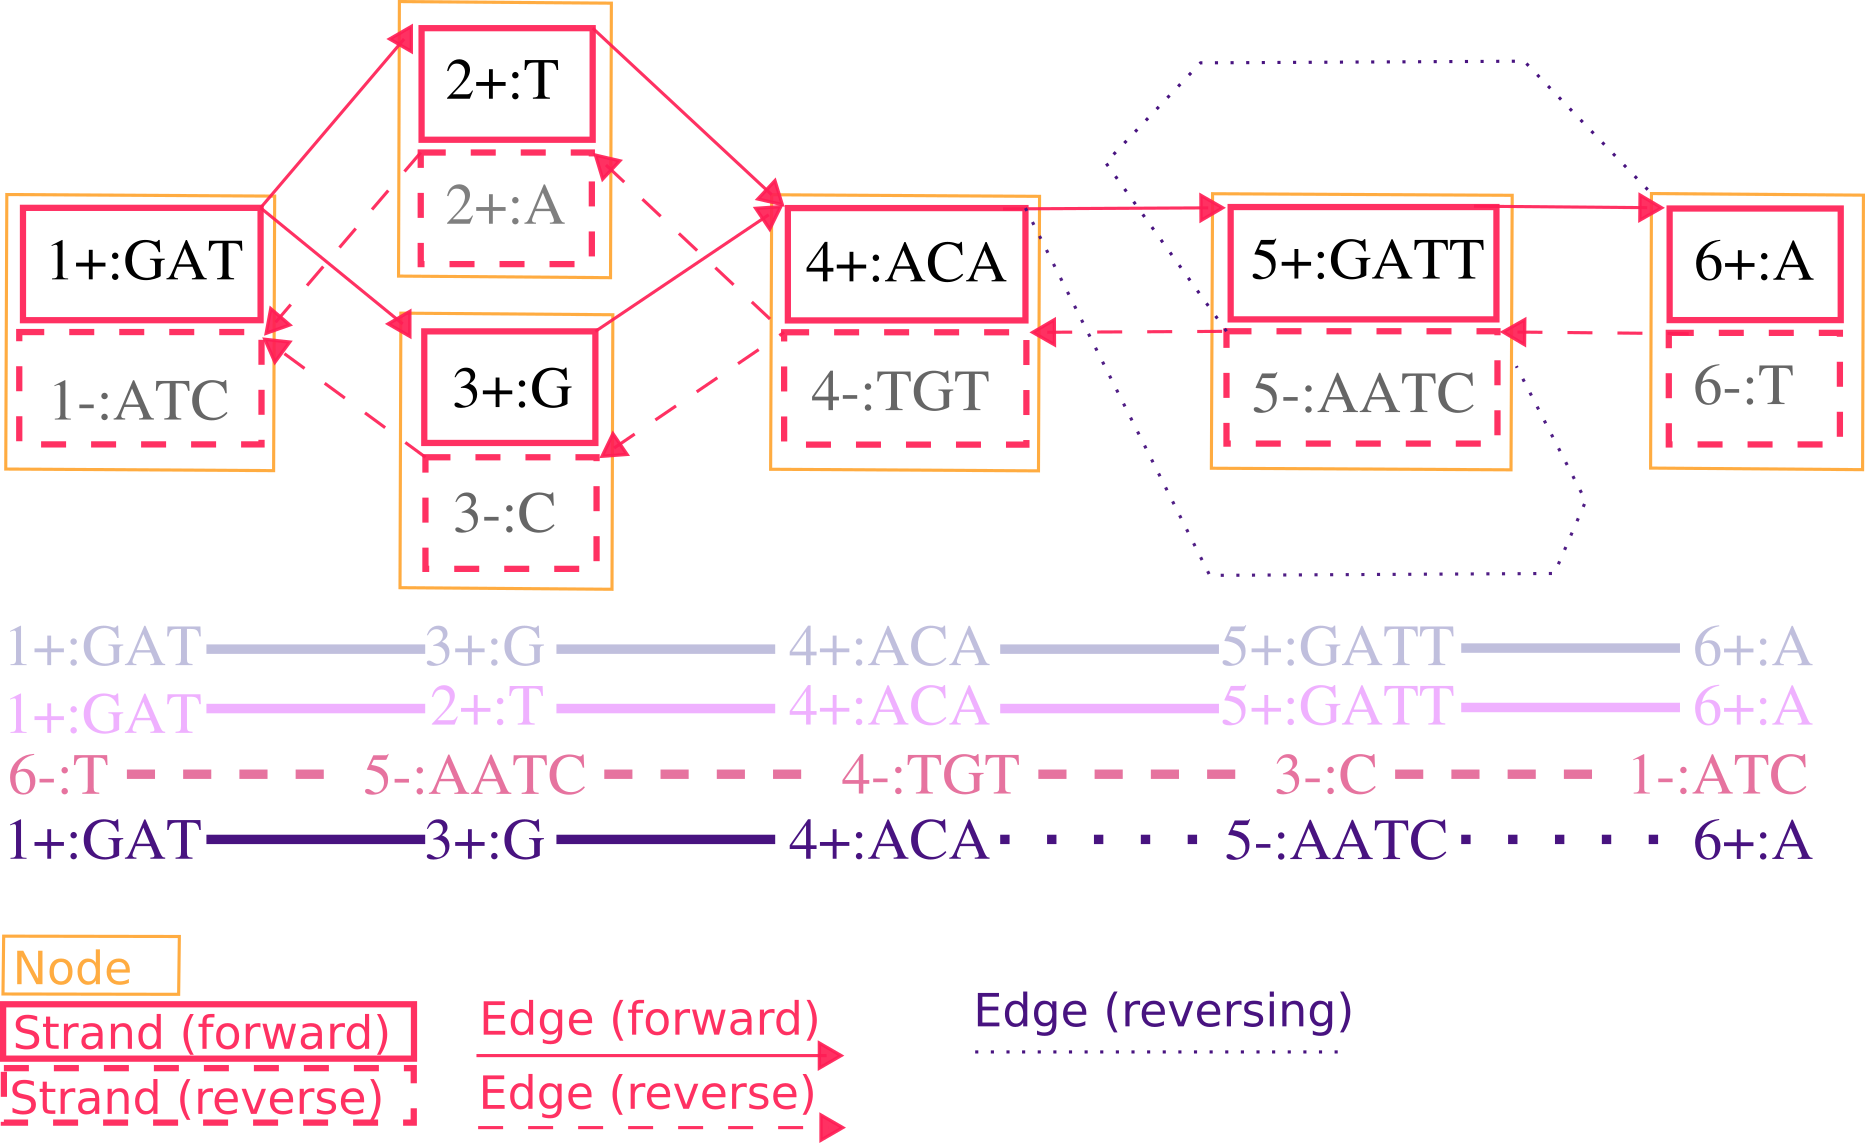
\includegraphics[width=0.5\textwidth]{handlefigures/GRaphchrXpaper.png}
	\end{center}
	\caption{{\label{fig:graph}
        \textbf{Entities in the bidirected sequence graph.}
        Top: a variation graph showing \emph{nodes} (yellow rectangles), each of which contain a forward and reverse \emph{strand} (red solid and dashed rectangles, respectively).
        Strands show the node identifier, the direction ($+$ or $-$), and the sequence of the strand.
        Note that reverse strands show the reverse complement sequence of the forward strand.
        All \emph{edges} are shown as connections between nodes, with forward-to-forward edges denoted by solid lines, and reverse-to-reverse edges denoted by dashed lines.
        Two edges that invert from forward to reverse and reverse to forward are shown with dotted lines.
        Edges run from the strand at their beginning to that at their end, as indicated by the arrowhead.
        Bottom: an illustration of four \emph{paths}.
        Each has a name, and can be referenced by a handle, which are omitted for brevity.
        Each path is shown in its natural direction as a series of connected \emph{steps} that refer to strands in the graph.
        The first two paths differ by a SNP, with one passing through \texttt{2+:T}, and the other through \texttt{3+:G}.
        The third path is the reverse complement of the first.
        The fourth is the same as the first, but contains an inversion, passing through \texttt{5-:AATC} rather than \texttt{5+:GATT}.
      }
    }
\end{figure}

\subsection{Graph implementations}

We consider five implementations of the \textsc{HandleGraph} model.
To ground our experimental results, here we we provide a high-level overview of each implementation.
Two implementations, \textsc{VG} and \textsc{XG}, have been described previously \cite{garrison2018variation,Garrison_2019}.
The others are combined in the \texttt{libbdsg} library (\url{https://github.com/vgteam/libbdsg}), which provides three concrete implementations: \textsc{HashGraph}, \textsc{ODGI}, and \textsc{PackedGraph}.
Each implementation represents a different tradeoff in terms of speed, memory use, and capabilities.
All of the implementations except \textsc{XG} are dynamic.
They support efficient addition and deletion of nodes, edges, paths, and steps, as well as some specialized methods such as splitting a node into multiple shorter nodes.
Table \ref{table:comparison} provides a high level summary of the differences between the \texttt{libbdsg} implementations.
%Readers seeking a precise description of each implementation should refer to developer documentation and code referenced in this section.

\subsubsection{\textsc{VG}}

We have extended the graph representation in \textsc{VG}, previously described in \cite{garrison2018variation}, to match the \textsc{HandleGraph} API.
The backing data structures used remain the same.
The graph entities are stored as objects in a backing vector, and referred to internally by hash tables that map between node identifiers and pointers into this vector.
Edges are indexed in a hash table mapping pairs of handles to edge objects.
Paths are stored in a set of linked lists, with a hash table mapping between nodes and path steps.
This arrangement was tenable for the early development of algorithms working on variation graphs.
Its inefficiency, caused by unnecessary overheads and data duplication, has resulted in significant difficulties for groups working with \textsc{VG}.
The other \textsc{HandleGraph} implementations respond to the limitations of this approach.
In version 1.22.0, vg was updated to use \textsc{HashGraph} (below) as the default format, though it remains compatible with all implementations described in this paper via the \textsc{HandleGraph} API.

%Its documentation can be found at \url{https://vgteam.github.io/vg/classvg_1_1VG.html}.

\subsubsection{\textsc{XG}}

\textsc{XG} was initially developed in response to the memory and runtime costs of \textsc{VG}, which prevent its application to large graphs.
It additionally provides positional indexes over paths that are required for read mapping and variant calling, and is the graph data model used in most established bioinformatic operations on variation graphs \cite{garrison2018variation,hickey2020genotyping}.
Unlike other \textsc{HandleGraph} implementations, \textsc{XG} is a static graph index.
This permits a more powerful set of efficient queries against the graph, especially for paths.
The encoding is designed to balance speed and low memory usage.
The topology of the graph is encoded in a single vector of bit-compressed integers, which promotes cache efficiency.
Rank and select operations on succinct bit vectors are used to provide random access over the variable-length records, which each encode a node's sequence, ID, and edges.
Embedded paths are encoded in variable-length integer vectors with Elias gamma encoding.
Rank and select operations on succinct bit vectors also provide queries by base-pair position along paths.
A detailed description of \textsc{XG} can be found in \cite{Garrison_2019}.
%Its documentation can be found at \url{https://github.com/vgteam/xg/blob/master/README.md}.

\subsubsection{\textsc{HashGraph}}

\textsc{HashGraph} is a relatively simple encoding, which is largely similar to the original \textsc{VG} graph.
As such, it can be seen as a streamlined point of comparison for the other new dynamic graph implementations.
However, the simplicity of this encoding has the benefit of allowing fast queries.
Thus, even though \textsc{HashGraph} still has relatively high memory requirements, it can still be useful in high memory compute environments or for small sequence graphs (such as subgraphs of genome graphs).

Like \textsc{VG}, \textsc{HashGraph} encodes the topology of the graph in a hash table indexed by node IDs.
However, what were separate hash tables in \textsc{VG} have been consolidated to avoid storing the keys multiple times.
The hash table it uses is a drop-in replacement for the equivalent standard library (STL) data structure, and has been shown to outperform it in empirical evaluations \cite{brehm2019hash}.
Each hash table entry contains the sequence, an adjacency list of the edges in two STL vectors, and a vector indicating the path steps that the node can be found on.
The graph's paths are represented using doubly-linked lists to support efficient modification at any position.

In contrast to the more memory-efficient implementations, all of these data structures support computation in their native in-memory representation.
Thus, the run time to access graph elements does not also include decompressing the data.
This is how \textsc{HashGraph} maintains its comparative speed advantage.

%\textsc{HashGraph} has speed and simplicity as its primary goal.
%The data structures used in HashGraph are largely similar to the original \textsc{VG} graph.
%It represents the graph nodes as a collection of node objects in a \texttt{sparsepp} hash table (selected due to our familiarity with the project and its ability to outperform the standard library \cite{brehm2019hash}), while paths are implemented as doubly-linked lists.
%Edges are recorded in vectors attached to each node that they connect.
%This adjacency list encoding is appropriate for genome graphs, which are typically very sparse.
%Each node object maintains a vector of pointers to the path steps that traverse it.
%Most of \textsc{HashGraph}'s component data structures are uncompressed STL objects which can be used efficiently in their native in-memory arrangement.
%\textsc{HashGraph} trades memory for time, and thus is most appropriate for small graphs (from small genomes or small regions of larger genomes) or for high-memory compute environments.
%Its implementation can be found at \url{https://github.com/vgteam/libbdsg/blob/master/include/hash_graph.hpp}.

\subsubsection{\textsc{ODGI}}

\textsc{ODGI} (Optimized Dynamic Graph Implementation) is based on a node-centric encoding that is designed to improve cache efficiency when traversing or modifying the graph.
This encoding is split between graph topology and paths, which is important for achieving a balance of runtime performance and memory usage on graphs with large path sets.
It uses delta encoding of edges and path steps to reduce the cost of representing graphs with local partial order and sparsity, both of which are common features of pangenome graphs.
\textsc{ODGI} is the default data model of the \textsc{ODGI} toolkit (\url{https://github.com/vgteam/odgi}), which provides high-level algorithms for graph manipulation and interrogation that are designed to work at the scale of large pangenomes.

In \textsc{ODGI}, each node $\mathcal{N} = ( \mathcal{B}, \mathcal{P} )$ is represented by a structure that contains a byte array $\mathcal{B} = (\mathcal{Q}, \mathcal{E})$ encoding its sequence and associated edges, and a compressed integer vector $\mathcal{P} = \mathcal{S}_1 \ldots \mathcal{S}_{s}$ describing the path steps that traverse it.
The full graph model is simply an array of these node records $\mathcal{G} = \mathcal{N}_1 \ldots \mathcal{N}_{|\mathcal{G}|}$ with some additional data structures to allow for random access of paths by name, and to maintain important statistics about the size of the graph, its node ID space, and its path set.

Each node's sequence $\mathcal{Q}$ is stored using a full byte per character at the start of the byte array $\mathcal{B}$.
This allows \textsc{ODGI} to represent protein as well as DNA sequence graphs, and allows for copy-free reference to the node sequences. % which can improve the performance of algorithms which interact with the sequence space of the graph.
The edges that begin or end at the node are recorded in the remainder of $\mathcal{B}$, encoded as deltas between the rank of the other end of the edge and the current node. 
%The set of $s$ steps traversing the node is recorded as an array of step records

\textsc{ODGI} stores paths as bidirectional linked lists that allow efficient insertions, deletions, and replacements of path steps.
These paths are encoded in a manner that exploits common properties of pangenome graphs, and node-level data structures are organized to support efficient operation on graphs with very deep path coverage.
The path steps $\mathcal{P} = \mathcal{S}_1 \ldots \mathcal{S}_{s}$ on each node are recorded as a series of records in a dynamic integer vector which is compressed so that only the largest integer entry is stored at full bit-width \cite{prezza2017framework}.
Each step $\mathcal{S} = (p_{id}, \delta_p, \delta_n, r_p, r_n)$ contains a path identifier $p_{id}$, references to the previous $\delta_p$ and next $\delta_n$ node ID and strands on the path encoded as deltas relative to the current node, and the ranks of the previous $r_p$ and next $r_n$ steps among the path steps on their respective nodes.
This path encoding scheme is similar to that used in the dynamic GBWT \cite{siren2020haplotype}, but differs in that the paths are not prefix-sorted.
%It is designed to exploit the sparse and orderable nature of genome graphs.
%If the graph is topologically sorted and node identifiers reflect this sort, the each path step will tend to connect nodes which have a small difference in identifier space.

%(e.g. from $n_{5} \to n_{7}$), then the maximum bit-width of the path vector will be low, resulting in good compression.



\subsubsection{\textsc{PackedGraph}}

\textsc{PackedGraph} is designed to have a very low memory footprint.
The backing data structures are implemented using bit-compressed integer vectors.
The bit-width of these vectors is chosen dynamically, starting with a bit-width of 1 and  then reallocating the vector at a higher width whenever an edit operation introduces an integer that is too large to be represented with the current width.
In the typical case that the value of $i$-th entry in the vector is $O(i)$, these reallocations have an  $O(1)$ amortized run time per edit.

Many of the integer vectors tend to also have entries that are highly correlated with their neighbors.
\textsc{PackedGraph} exploits this characteristic to achieves greater compression by only storing one entry per fixed-size window at full bit-width.
 The rest of the entries are stored in a separate integer vector and expressed as a difference from that entry.
 Since the differences within a window tend to be small, this encoding keeps the bit-width for each window small as well.

The data associated with each node is recorded in several compressed integer vectors (at the same index in each).
Contrast \textsc{XG} and \textsc{{ODGI}}, which encode data in a single vector to improve cache efficiency.
Recording only one homogenous data type in a vector increases the correlation between neighboring values, which in turn improves compression.
The adjacency list for the graph, the steps that each node is found on, and the paths themselves are represented using linked lists.
The linked lists reside within the same bit-compressed integer vectors, where pointers are created by treating some integer entries as indexes into the vector itself.
This pointer encoding also guarantees the technical condition that accessing the $i$-th entry is $O(i)$.
The linked lists that occur on every node (the adjacency lists and node step lists) are included in a single vector across all nodes.
This serves two purposes.
First, the windowed compression scheme in the integer vectors is inefficient if lists are smaller than the window size, as is often the case.
Second, due to the local partial order that is found in many pangenome graphs, neighboring nodes often connect to the same nodes and are found on the same paths as each other.
Thus, the values they store are also highly correlated.
%Most of its component data structures are---conceptually speaking---linked lists.
%However, they are implemented using vectors of bit-compressed integers, where pointers are produced by treating some of the integer entries as indexes into the vector that contains them.
%The bit-width can be determined dynamically.
%Doing so does not affect the amortized asymptotic run time of graph operations in the typical case that the value of $i$-th entry in the vector is $O(i)$.
%The vector uses a windowed bit compression scheme in which only one value within a window is maintained at its full bit-width.
%The remaining entries are represented as differences from this value.
%In the typical case where adjacent entries in the vector are highly correlated, this helps keep the bit-width low and the compression high.
%Its implementation can be found at \url{https://github.com/vgteam/libbdsg/blob/master/src/packed_graph.cpp}.

%Longer-range jumps do occur, but they tend to be more rare.
%Modifying path step records can be expensive, but when the number of traversing paths is relatively small, it remains in higher caches and can be accomplished efficiently.

\begin{table}
\ssp
  \centering
\begin{tabular}{>{\raggedleft\arraybackslash}p{.23\columnwidth}|>{\raggedright\arraybackslash}p{.2\columnwidth}>{\raggedright\arraybackslash} p{.2\columnwidth}>{\raggedright\arraybackslash} p{.24\columnwidth}}
\textbf{Model} & HashGraph & ODGI & PackedGraph  \\
\hline
\textbf{Design goal} & Simplicity, speed & Memory efficiency & Balanced speed/memory \\
\Xhline{0.1\arrayrulewidth}
\textbf{Topology data structure} & Hash table & Single integer vector & Several integer vectors \\
\Xhline{0.1\arrayrulewidth}
\textbf{Topology compression} & None & Delta encoding & Windowed bit compression \\
\Xhline{0.1\arrayrulewidth}
\textbf{Sequence compression} & None & None & Bit compression \\
\Xhline{0.1\arrayrulewidth}
\textbf{Pointer encoding} & Memory addresses & Delta-encoded ranks & Vector indexes \\
\hline
\end{tabular}
\caption{
  \textbf{Comparison of features between libbdsg graph implementations.}
  The three graph implementations all use adjacency lists to encode graph topology and linked lists to encode paths. 
  The differences in encoding these structures reflects different design goals for each implementation.
}
\label{table:comparison}
\end{table}


\subsection{Python binding}

We have implemented a Python binding to the graph implementations in \texttt{libbdsg} using Pybind11 \cite{pybind11}.
This allows the data structures to be used in Python applications, significantly lowering the barrier-to-entry for pangenomic application developers.
This functionality is documented at \url{https://bdsg.readthedocs.io}, including a tutorial.
This documentation also serves as useful introduction to the \textsc{HandleGraph} API.
%The full implementation of \textsc{ODGI} can be found at \url{https://github.com/vgteam/libbdsg/blob/master/src/odgi.cpp}.

\subsection{Code availability}

Both \texttt{libhandlegraph} and \texttt{libbdsg} are open source under an MIT License.
They are available on GitHub at \url{https://github.com/vgteam/libhandlegraph} and \url{https://github.com/vgteam/libbdsg}.
Documentation for the two libraries, including the C++ handle graph API, \textsc{HashGraph}, \textsc{ODGI}, and \textsc{PackedGraph}, is available at \url{https://bdsg.readthedocs.io} alongside the documentation for the Python binding.
%\begin{figure}[!tpb]%figure2
%%\centerline{\includegraphics{fig02.eps}}
%\caption{Caption, caption.}\label{fig:02}
%\end{figure}


\section{Evaluation}

\subsection{Human genome with structural variants}

\begin{figure}
	\begin{center}
		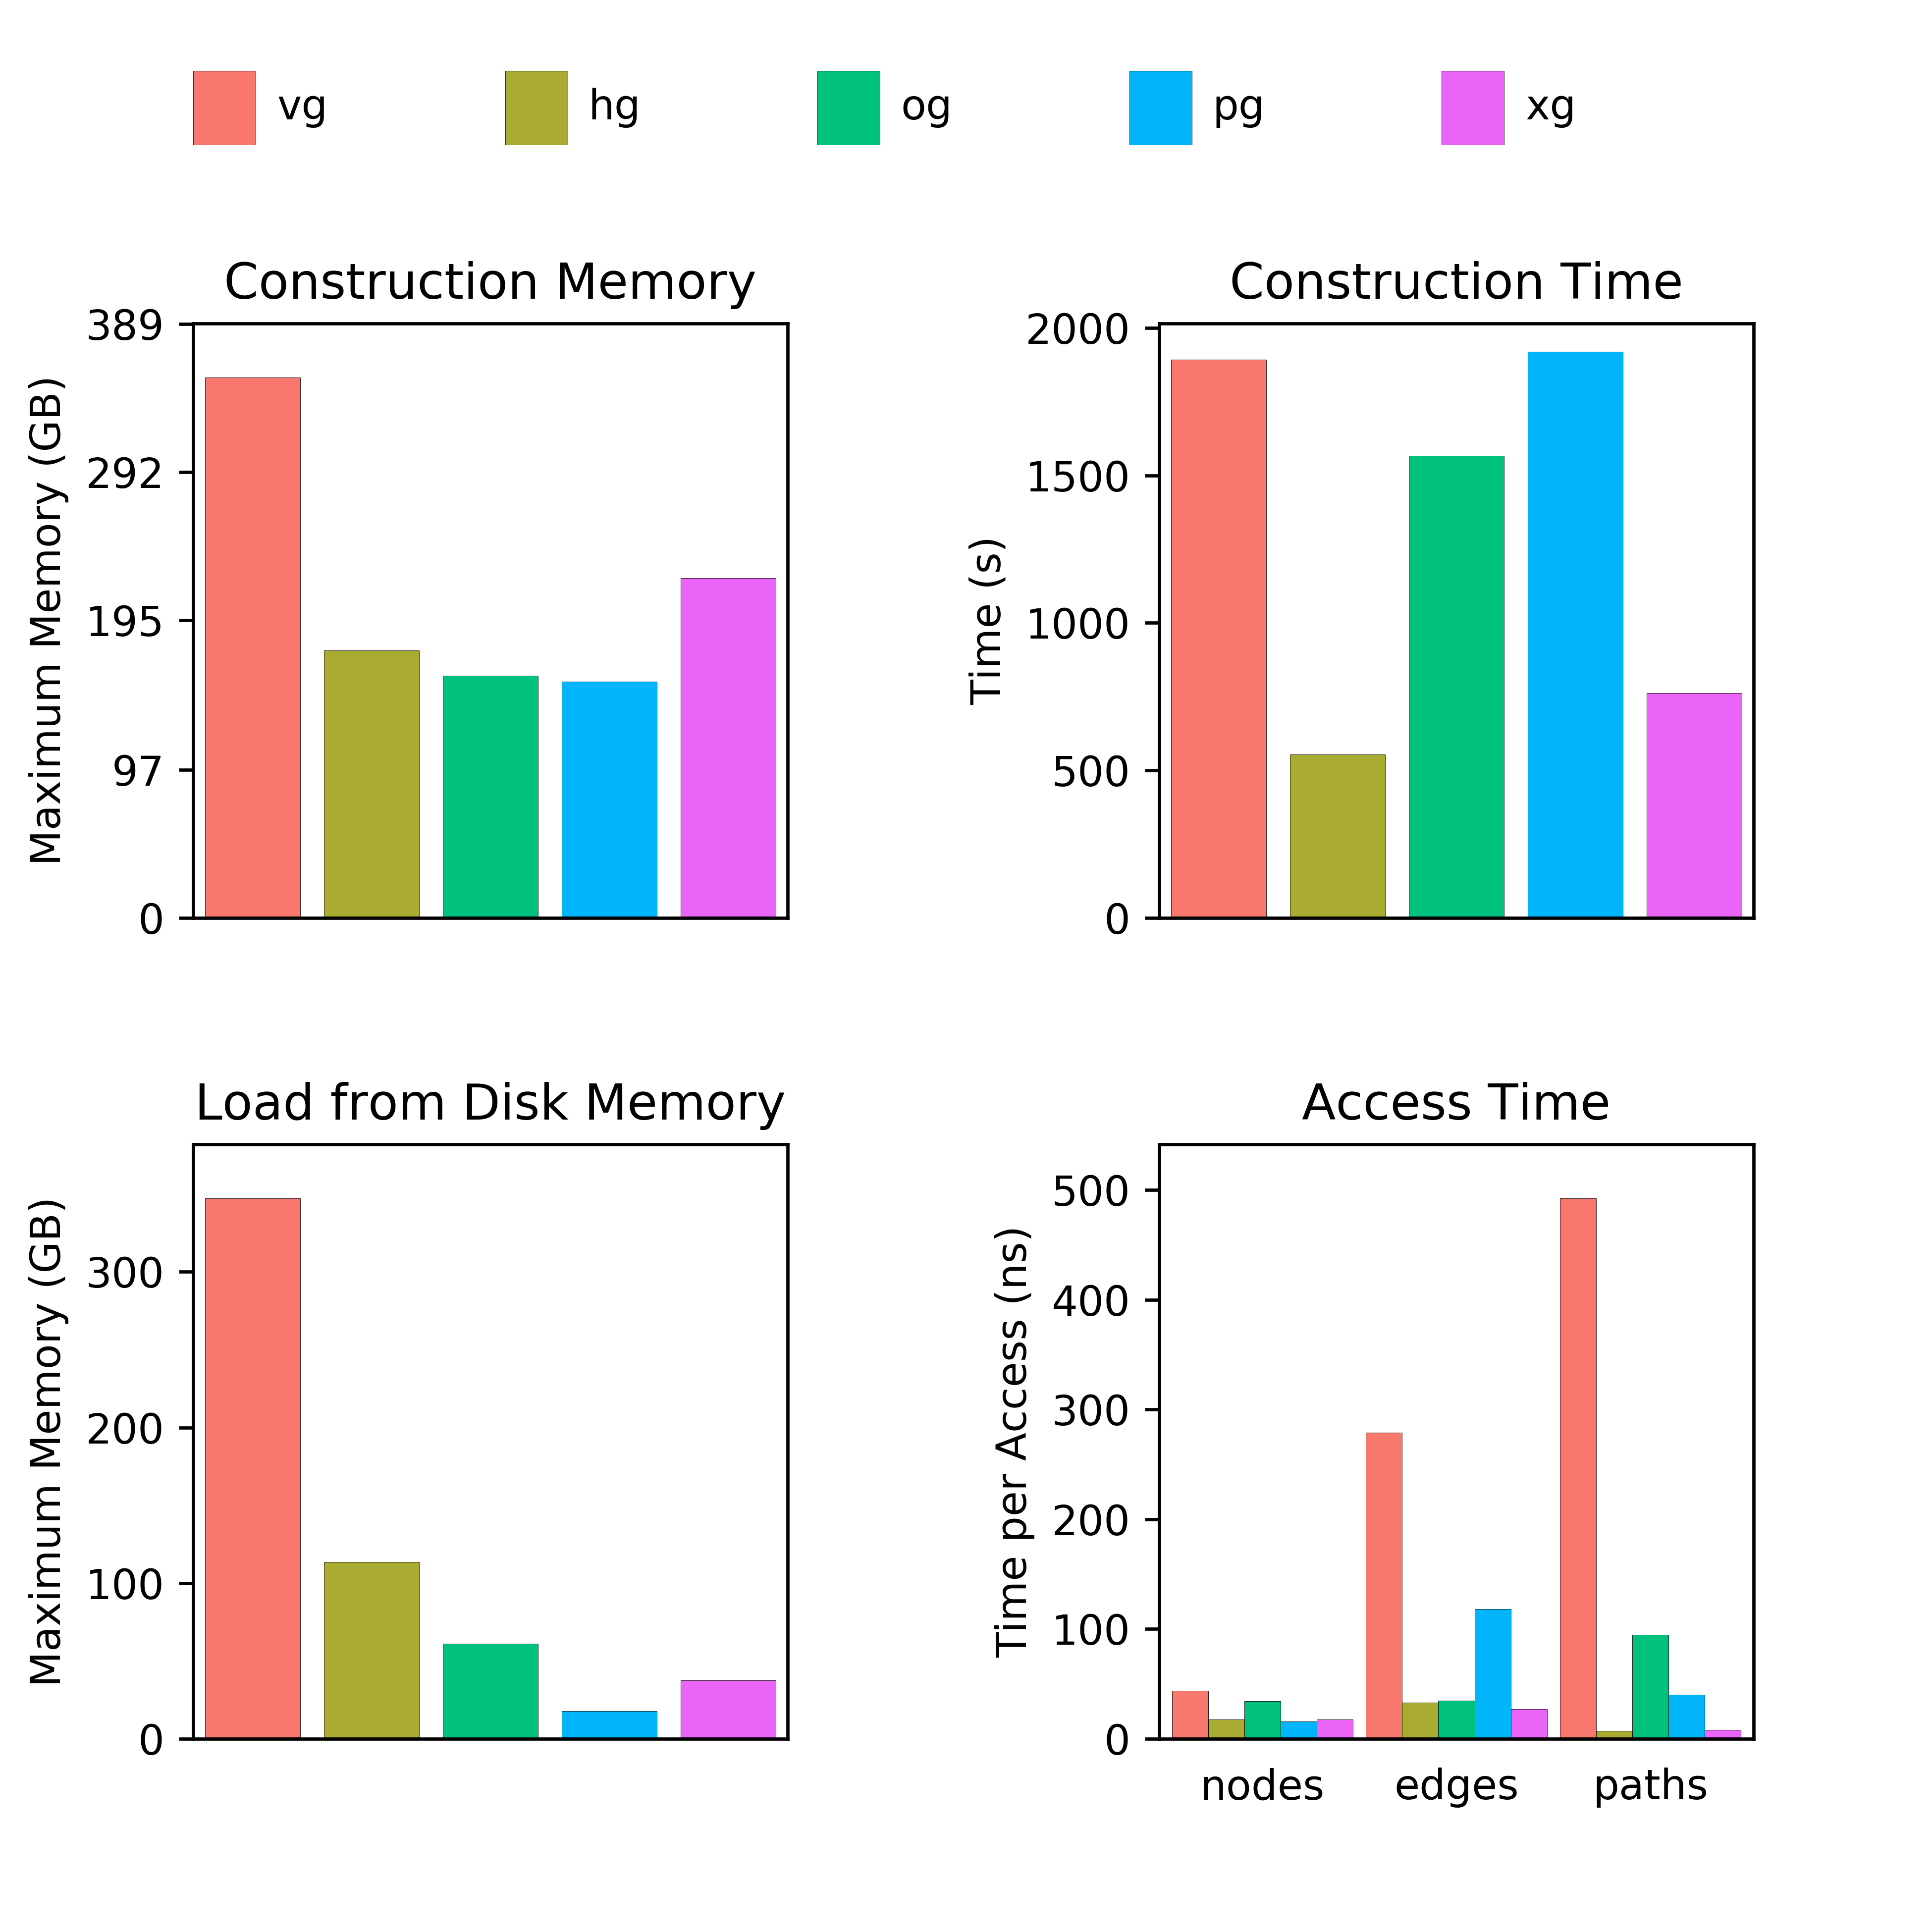
\includegraphics[width=0.5\textwidth]{handlefigures/HGSVC_sorted_gfa.png}
	\end{center}
	\caption{{\label{fig:hgsvc}
        \textbf{Performance on a graph of structural variants from the HGSVC.}
        Abbreviations used here and in subsequent figures and tables: vg = \textsc{VG}, hg = \textsc{HashGraph}, og = \textsc{ODGI}, pg = \textsc{PackedGraph}, xg = \textsc{XG}.
        All four new graph implementations compare favorably to \textsc{VG}.
        \textsc{PackedGraph} tends to be the most memory efficient, \textsc{HashGraph} tends to be the fastest, and \textsc{ODGI} is balanced in between.
        \textsc{XG} provides good performance on both memory usage and speed, but it is static.
        }
      }
\end{figure}

We measured the core operation performance of the four graph implementations and the graph class from the popular \textsc{VG} software (as implemented prior to version 1.22.0).
In particular, we measured 1) memory usage to construct a graph, 2) time to construct a graph, 3) memory usage to load an already-constructed graph, and 4) time to access nodes, edges, and steps of a path.
These access operations are one of the major drivers of run time in pangenomic applications, such as \textsc{VG}'s read mapping algorithm. 
Accesses were performed with a single thread, and the reported access time is the average time taken when accessing each graph element sequentially.
All evaluations were performed on a~3.1~GHz Intel Xeon Platinum~8000~series processor.
The presented results are from a graph describing the structural variants of the Human Genome Structural Variation Consortium \cite{chaisson2019multi}, which was recently used to genotype structural variants \cite{hickey2020genotyping}.
Specifically, the graph consists of the GRCh38 primary scaffolds and 72,485 indel variants ranging in size from 50~bp to 76~kbp.
The results generally match our expectations based on the implementations' design goals (Figure \ref{fig:hgsvc}).

\subsection{Genome graph collection}

\begin{figure}
  \centering
  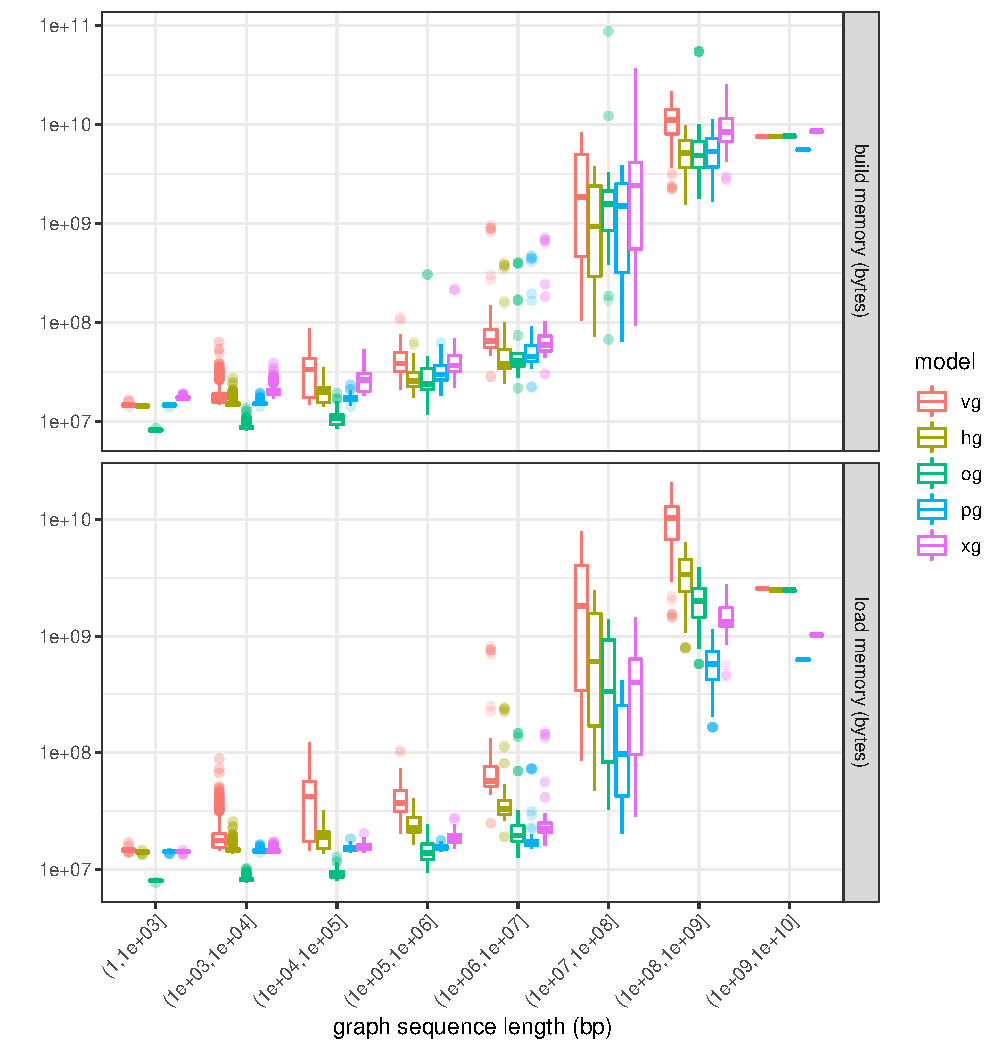
\includegraphics[width=0.5\textwidth]{handlefigures/build_and_load_memory_boxplot.pdf}
  \caption{
    \label{fig:prof1}
    \textbf{Memory requirements for model construction and loading.}
    Memory costs versus graph sequence size for the graph collection, colored by \textsc{HandleGraph} model.
    The memory requirements for graph construction tend to be higher than those for loading the graph model.
    All methods show fixed overheads of several megabytes, seen in the flat tail to the left of both plots.
    Outside of this region, all methods show roughly linear scaling in both build and load costs per input base pair.
    The relative differences in memory costs appear to be stable between different methods across many orders of magnitude in graph size.
    }
\end{figure}
 
\begin{figure}
  \centering
  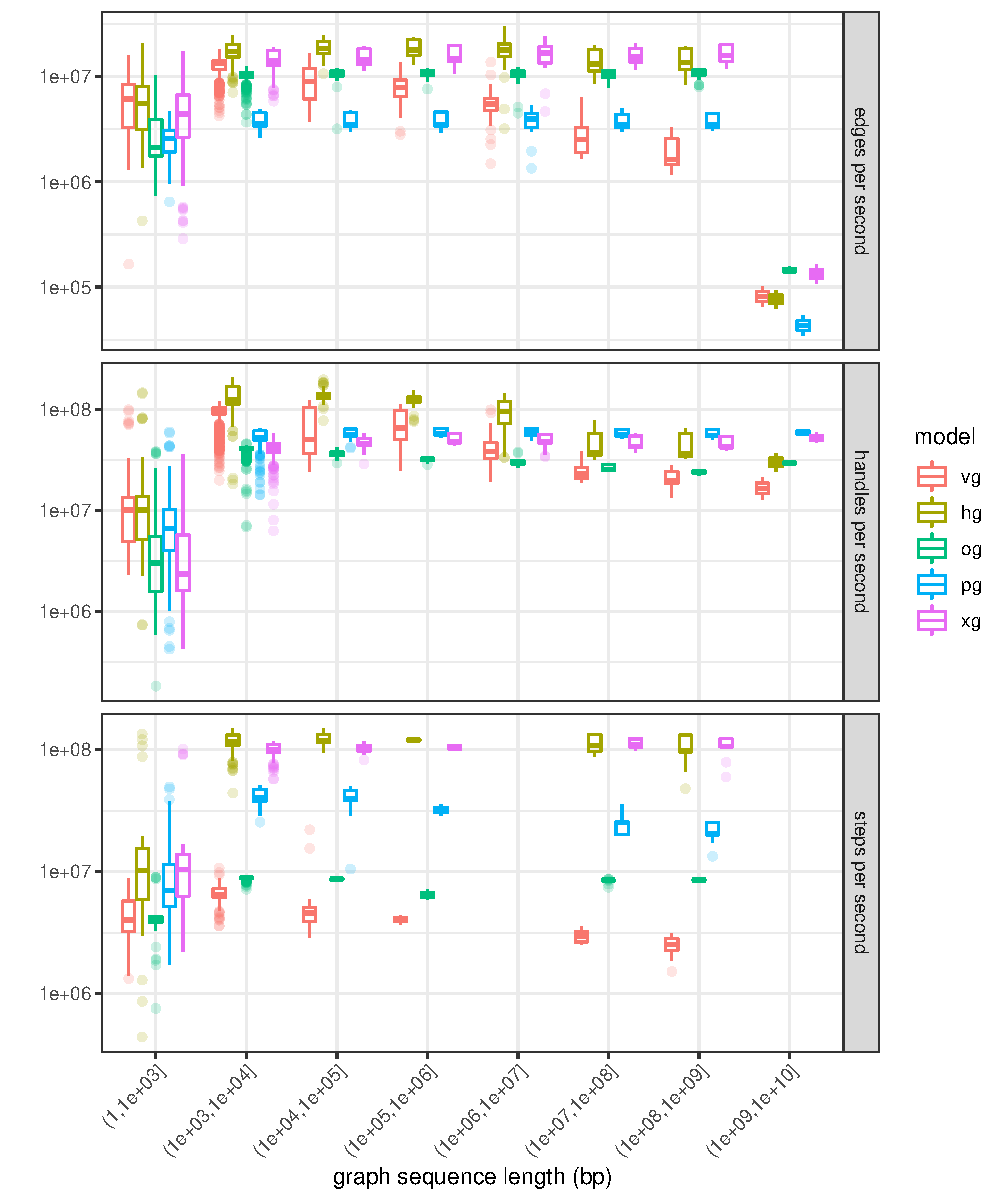
\includegraphics[width=0.5\textwidth]{handlefigures/iteration_per_second_boxplot.pdf}
  \caption{
    \label{fig:prof2}
    \textbf{Graph element enumeration performance.}
    Iteration performance for edges, nodes, and path steps for the full graph collection, shown in terms of elements per second.
    \textsc{HashGraph} provides the highest performance for all element iteration types on smaller graphs, but this performance falls of with larger graphs, presumably due to scaling properties of the backing hash tables.
    The same pattern can be seen for \textsc{VG}, although the overall performance is worse.
    Although it has the worst edge iteration performance, \textsc{PackedGraph} provides good performance on node and path step iteration.
    The relative path encoding in \textsc{ODGI} yields poor performance on path iteration, and node decoding overheads appear to reduce its node iteration performance, but it has good graph topology traversal performance, perhaps due to cache efficiency of the edge encoding.
    \textsc{XG} provides excellent iteration performance in all cases.
    }
\end{figure}

To compare the methods' performances across a wide variety of different graphs, we applied each to a collection of 2299 graphs collected during our research on graphical pangenomics.
For each graph and graph implementation, we measured the same metrics described in the previous section as well as various graph properties including size, edge count, cyclicity, and path depth.
We summarize these results in Figures \ref{fig:prof1} and \ref{fig:prof2}.

For graph construction and loading, we observe similar trends as for the HGSVC graph.
\textsc{VG}'s performance in terms of memory usage is very poor, both during construction and load.
For construction and load, all models exhibit largely linear scaling characteristics, outside of very small graphs where static memory overheads dominate.
\textsc{PackedGraph} yields the best memory performance for larger graphs (which are mostly the chromosomes of the 1000 Genomes Project graph), while for the medium-sized graphs in the collection ($\sim$1~Mbp), \textsc{ODGI} requires less memory.

For graph queries and iteration, the relative performance of the models is largely maintained across the entire range of graph sizes.
However, we observe that the hash-based models (\textsc{VG} and \textsc{HashGraph}) have very good performance for smaller graphs (in handle and edge enumeration) but decrease in throughput as the graph size increases.
Smaller, less dramatic decreases in performance can be seen for the other implementations.
For path enumeration, the highest-performing methods are \textsc{XG} and \textsc{HashGraph} at approximately 10 times faster than \textsc{ODGI}, whose relative path storage is costly to traverse.

\subsection{1000 Genome Project chromosome graphs}

Variation graphs built from the 1000 Genomes Project (1000GP) variant catalog and the human reference genome have fairly homogenous and regular features.
In addition, they have connected components of very different sizes, each corresponding to a chromosome.
This provides a natural, fairly controlled means to explore the scaling behavior of our data structures.
Moreover, graphs of this form are seeing increasing use in variant-aware resequencing analyses \cite{crysnanto2020bovine}.
Thus, the performance of data structures on these graphs is of general interest.

\begin{figure}[p]
  \centering
  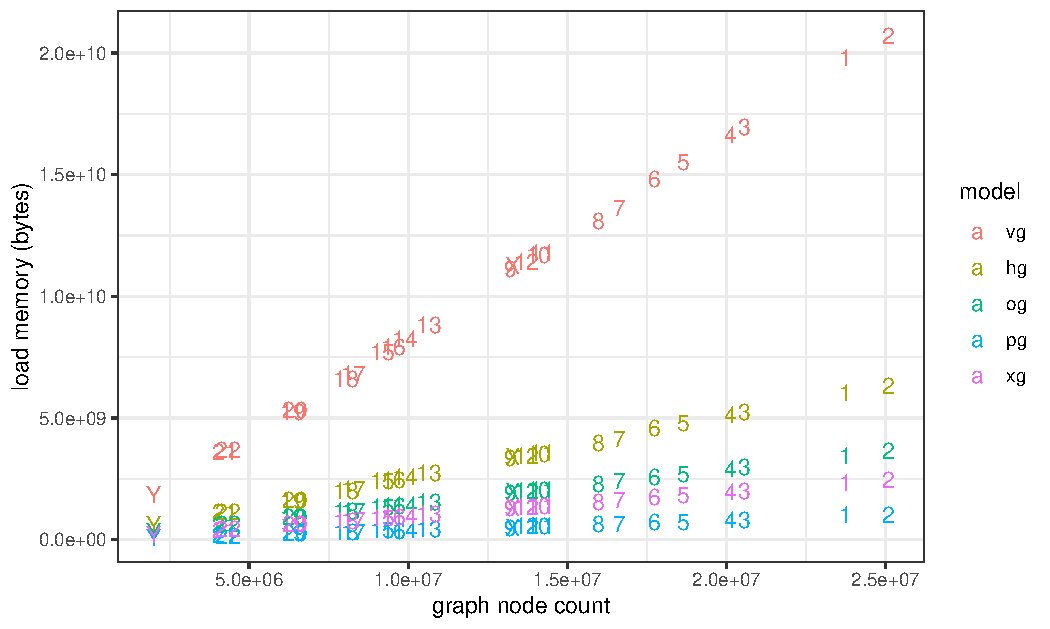
\includegraphics[width=0.5\textwidth]{handlefigures/1000gp_chroms_node_count.pdf}
  \caption{
    \label{fig:1000GPchroms}
    \textbf{Load memory versus node count for chromosome graphs built from 1000 Genomes Project variants and GRCh37.}
    For each method, memory requirements are more strongly correlated with the number of nodes in the graph ($R^2 =$ 0.998) than with the graph sequence length ($R^2 =$ 0.986).
    Although the memory requirements are dominated by graph sequence size, node count will increase with variant density.
    Methods generally incur an overhead for each node that is larger than the sequence length.
    Linear scales clarify that the absolute difference in performance between \textsc{VG} and the other methods is substantial.
    }
\end{figure}

We first evaluated the scaling performance of the various \textsc{HandleGraph} implementations relative to node count for each of the nuclear chromosomes in the 1000GP (Figure \ref{fig:1000GPchroms}).
We find that for all methods, load memory scales almost perfectly with node count, with an average $R^2 = 0.998$.
Due to differences in variant density among the chromosomes, the average correlation relative to sequence length is lower ($R^2 = 0.986$).

\begin{table}
\ssp
  \centering
\begin{tabular}{c||r|r|r|r|r}
 & \multicolumn{1}{c|}{Build} & \multicolumn{1}{c|}{Load} & \multicolumn{3}{c}{Iteration rate (millions)} \\
\multicolumn{1}{c||}{Model} & \multicolumn{1}{c|}{B/bp} & \multicolumn{1}{c|}{B/bp} & \multicolumn{1}{c|}{Node/s} & \multicolumn{1}{c|}{Edge/s} & \multicolumn{1}{c}{Step/s} \\
\hline
vg &   80.2 &                77.2$\ \ $  &              24.6 &                  2.8 &               2.9 \\
hg &   36.7 &                23.9$\ \ $  &              59.5 &                 18.9 &              \textbf{127.2} \\
og &   \textbf{30.3}  &   13.7$\ \ $  &              24.1 &                 11.5 &              8.2 \\
pg &   37.6 &                 \textbf{3.80}  &   \textbf{63.7} &   4.6 &                24.3 \\
xg &   54.3 &                9.31  &               54.2 &                 \textbf{20.5} & 117.0 \\
\end{tabular}
\caption{
  \textbf{Performance on 1000 Genomes Project chromosome graphs.}
  Average build memory, load memory, and iteration times for graph elements for the chromosome-level graphs built from all the variants in the 1000 Genomes Project and the GRCh37 reference genome against which the variant set was originally reported.
  \textsc{VG} requires~$\sim$~20 times as much memory to load the graphs as \textsc{PackedGraph}, while even the most costly \texttt{libbdsg} model (\textsc{HashGraph}) requires~$\sim$~1/3 as much memory.
  In these graphs, \textsc{ODGI} provides the lowest performance for handle iteration.
  However, in all other metrics, \textsc{VG} performs much worse than the other models.
}
\label{table:1000GPchroms}
\end{table}

In Table \ref{table:1000GPchroms}, we report the average memory performance of the methods relative to graph sequence length, and also the iteration performance in terms of elements per second.
We find that the best-performing method in terms of memory usage is \textsc{PackedGraph}, which consumes around $1/20$th the memory of \textsc{VG} per base-pair of graph in the 1000GP set.
Moreover, it provides much better iteration performance for nodes (handles), edges, and path steps.
\textsc{HashGraph} and \textsc{XG} have similar iteration performance, but \textsc{XG}, by virtue of its use of compressed, static data structures, requires less than half as much memory.
\textsc{ODGI} optimized for efficient dynamic operations on graphs with higher path coverage, and in general is not as performant as other methods on this set.


\section{Discussion}

We have presented a set of simple formalisms, the \textsc{HandleGraph} abstraction, which provides a coherent interface to address and manipulate the components of a genome variation graph.
To explore the utility of this model, we implemented data structures to encode variation graphs and matched them to this interface.
This allowed us to directly compare these \textsc{HandleGraph} implementations on a diverse set of genome graphs obtained during our research.
These experiments reveal that genome graphs need not pay the computational expense of the early versions of \textsc{VG}.
The best-performing models require an order of magnitude less memory than \textsc{VG} while providing higher performance for basic graph access operation and element iteration.
For these reasons, \textsc{VG} has transitioned to using these newer graph implementations. 

The efficiency of these methods and their encapsulation within a coherent programming interface will support their reuse within a diverse set of application domains.
Variation graphs have deep similarity with graphs used in assembly; these libraries could be used as the basis for assembly methods.
They could also be used for genotyping and haplotype inference methods based on graphs \cite{garg2018graph}.

Ongoing work is establishing large numbers of highly-contiguous whole genome assemblies for humans (\url{https://humanpangenome.org/}).
Improvements in sequencing technology are likely to make such surveys routine.
It is natural to consider a pangenome reference system, based on the whole genome alignments of such assemblies, as the output of these pangenome projects.
Recent results demonstrate that many basic bioinformatic problems can be generalized to operate on such structures.
Should these pangenome representations become common or standard, then variation graph data structures like those we have presented here will form the basis for a wide range of pangenomic methods.

\chapter{Automated index coordination within the VG toolkit}
\label{chapter:autoindex}

\section{Introduction}

Since its initial publication, VG\cite{garrison2018variation} has become one of the most widely used software tools for graph-based pangenomics. Although the VG toolkit has many functionalities, it is best known for read mapping to sequence graphs. Indeed, VG contains three separate mapping algorithms:

\begin{enumerate}
\item vg map: the original, highly accurate mapping algorithm\cite{garrison2018variation}
\item vg giraffe: the much faster and still accurate haplotype-based mapping algorithm\cite{siren2020genotyping}
\item vg mpmap: the splice-aware RNA-seq mapping algorithm that can produce multipath alignments\cite{sibbesen2021haplotype}
\end{enumerate} 

Each of these mapping tools depends on a sizeable body of research in specialized data structures and algorithms\cite{siren2017indexing,chang2020distance,siren2020haplotype,eizenga2020efficient}. As a result, they each require a different set of indexes to be built before mapping. Historically, navigating the indexing process has been a pain point for VG's users. The indexing algorithms and their documentation are spread across several VG subcommands, and the steps need to be applied in a specific order to produce valid, usable results.

The VG autoindex utility is designed to alleviate the pain involved in this process. Rather than having an interface based on which index the user wants to produce, it has an interface based on which mapping tool they want to run. The inputs are all common interchange formats like FASTA, VCF, and GFA. Internally, autoindex has the logic of the VG team's best practice indexing pipelines built in. Power users might still find need for the individual indexing subcommands, but the goal of autoindex is to produce indexes for any common use case in a single, easily-understood shell command.

\section{Methods and implementation}

The central abstraction in autoindex is the \emph{recipe graph} (Figure \ref{fig:recipe_graph}). This graph is a bipartite directed acyclic graph with two classes of nodes: \emph{file nodes} and \emph{recipe nodes}. The file nodes correspond to either input data (provided in interchange formats) or to VG indexes. The recipe nodes correspond to algorithms to produce VG indexes from a set of file nodes, which may correspond either to input data or to intermediate indexes. Each recipe node expresses a many-to-many relationship between file nodes: the recipe may require multiple files as input, and it may produce multiple files as output. This graph is hard-coded into VG. Each of the constituent recipes is based on the best practices developed for the VG developers' own pipelines.

\begin{figure}[h]
  \centering
  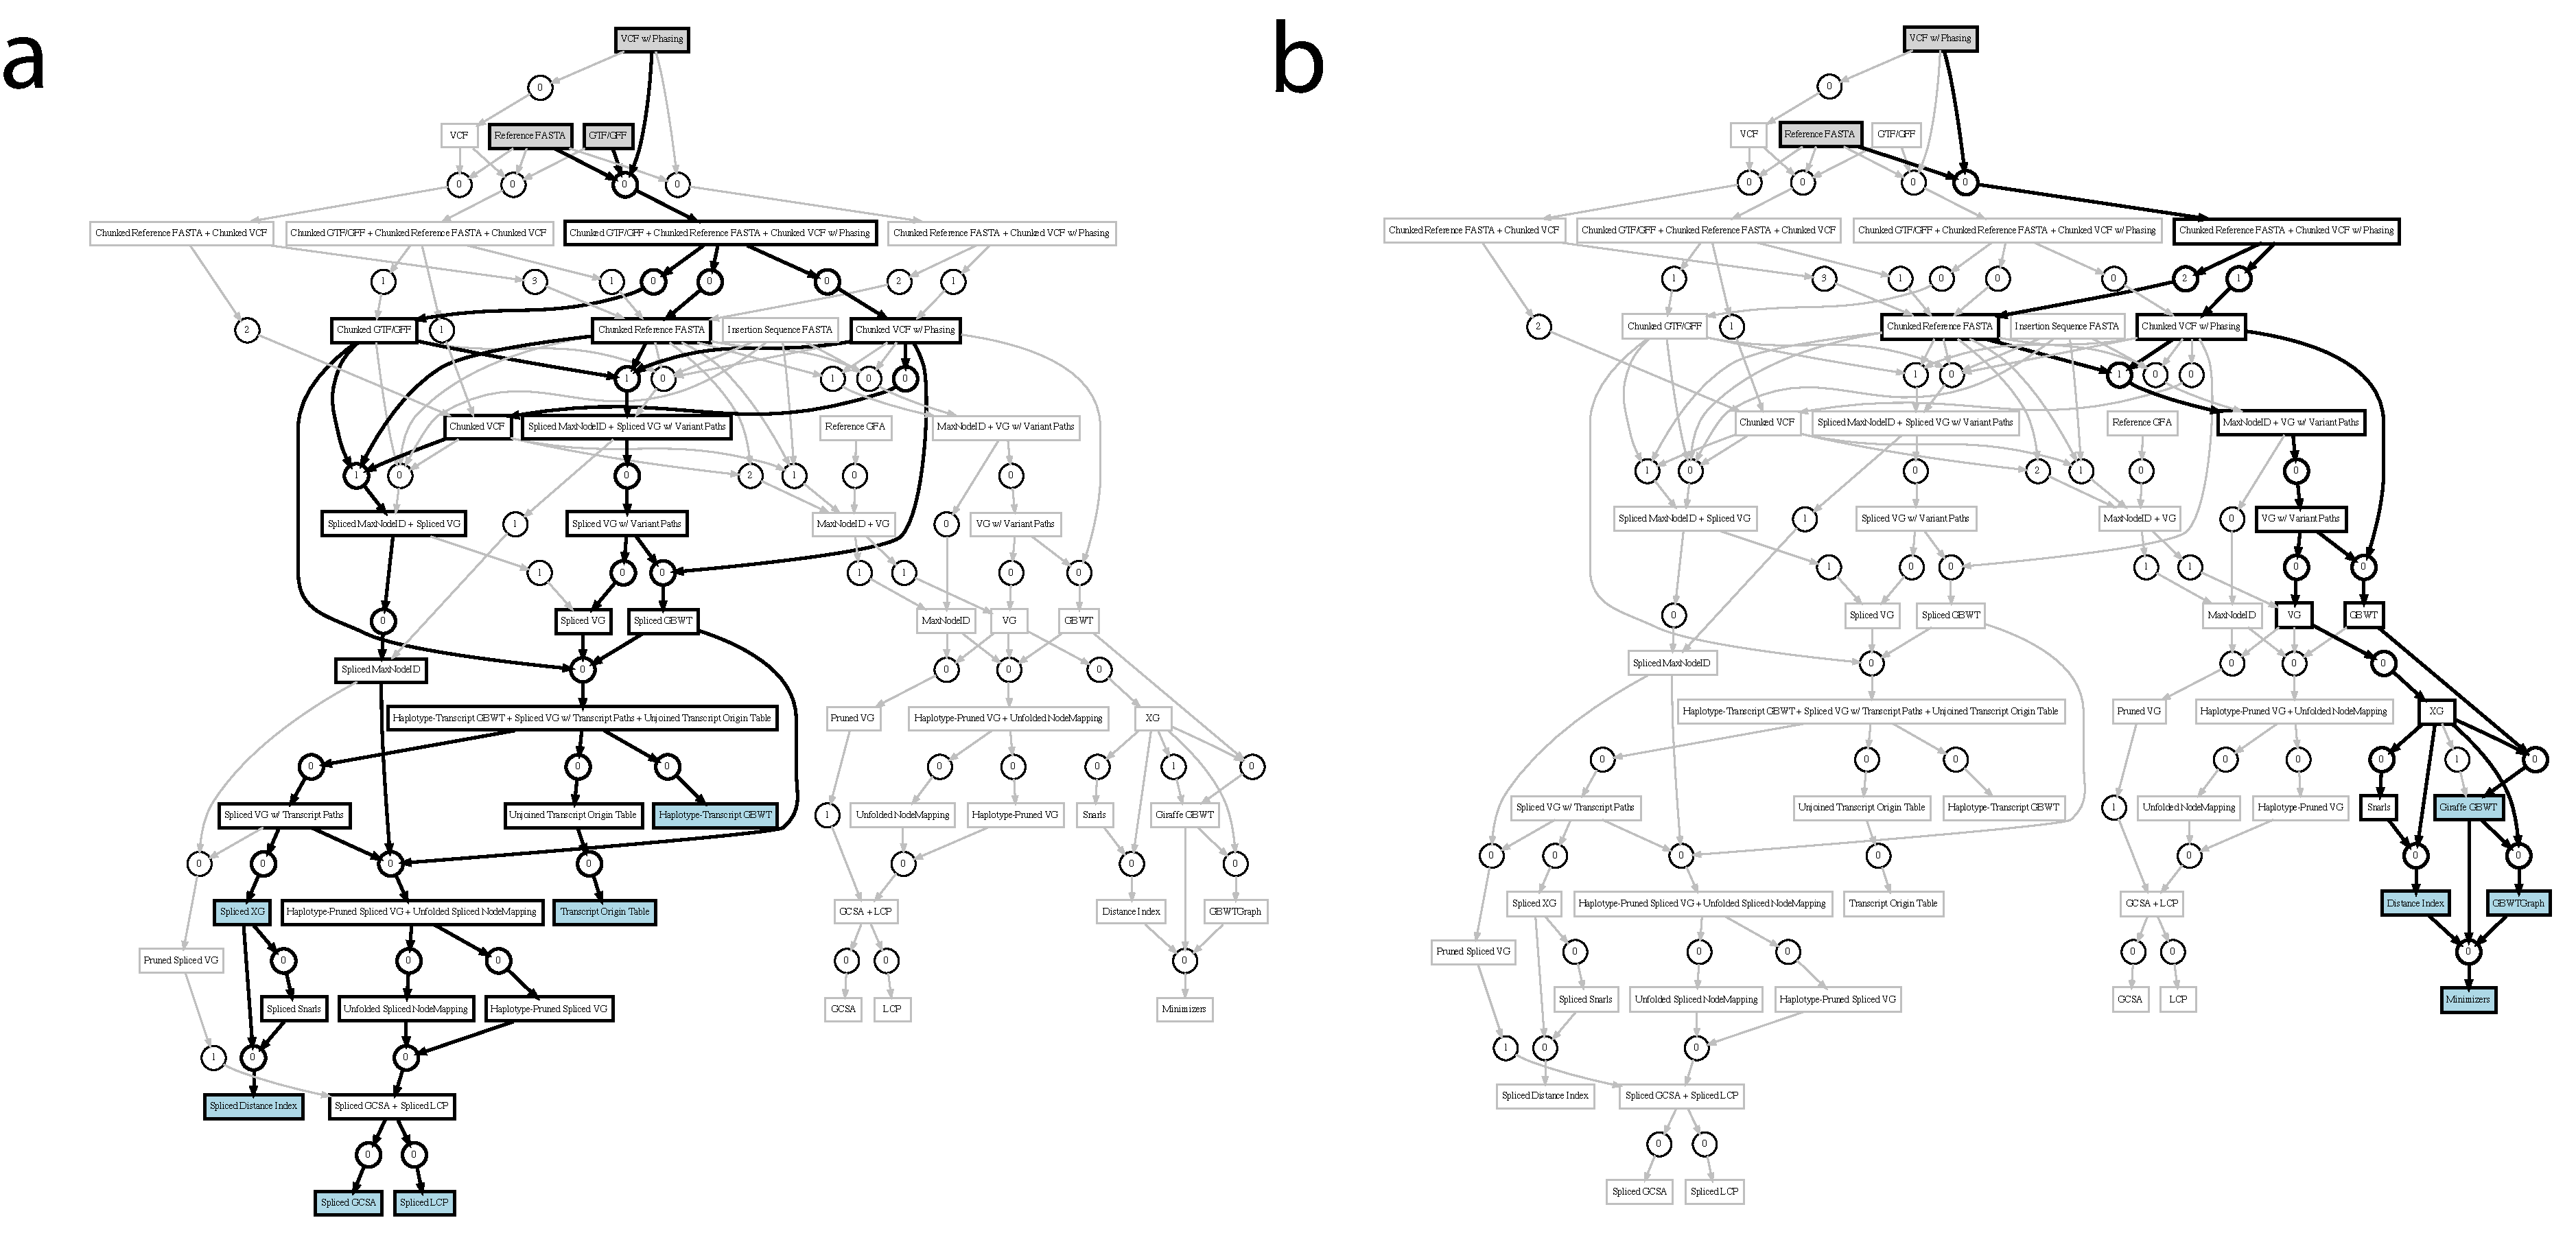
\includegraphics[width=\textwidth]{autoindexfigures/recipe_graph.pdf}
  \caption{
    \label{fig:recipe_graph}
    \textbf{Two plans in the recipe graph.}
    Plans for the indexes required by \textbf{a} \texttt{vg mpmap} and \texttt{rpvg} and by \textbf{b} \texttt{vg giraffe} are highlighted in the recipe graph. Rectangular nodes correspond to indexes or data files, and circular nodes correspond to recipes. Lower numbers on the recipe nodes indicates higher priority. Gray shading indicates provided data, and blue shading indicates the target indexes being constructed.
    }
\end{figure}

\subsection{Planning index construction pipelines}

The autoindex utility is equipped with an algorithm that determines the best pipeline, referred to as a \emph{plan}, to construct any index in the recipe graph using a given set of inputs. Recipes are labeled with a priority level: a total ordering that is used to determine which recipe is preferred when more than one recipe could be used to construct the same index. A plan is considered suboptimal whenever a higher priority recipe could be used to construct any of its indexes. In general, higher priority recipes correspond to improved versions of indexes that can be constructed using additional information. For example, path queries can be improved if the variants in a VCF file are phased\cite{siren2020haplotype}. 

The planning algorithm uses an exhaustive search to find the optimal plan. To begin, all file nodes that have been provided as input data are labeled complete. The search begins by initializing a queue with the target index. In each iteration, the lowest-valued file node (according to the partial order defined by the recipe graph, which is a DAG) on the queue is de-queued. If this file node is labeled complete, nothing is added to the queue. Otherwise, the file node's highest-priority recipe is added to the plan and the inputs for that recipe are added to the queue. If there is no recipe to construct the index, the search backtracks through the plan marking recipes impossible until finding a file node that has remaining recipes that have not yet been marked impossible. This algorithm is exponential in the worst case. However, the recipe graph is fairly small, and in practice the planning process takes a negligible amount of time.

The indexes required for each of VG's mapping tools are hard-coded into the autoindex utility. This is what allows autoindex to provide its tool-oriented interface. The user requests whatever indexes are required to use a tool. The autoindex utility then looks up a list of indexes that are sufficient to run that tools and finds the optimal plan to construct each of them based on the available data. The individual index's plans are then merged into one plan, and the pipeline is executed. 

This design has several benefits. If pipelines were described explicitly, it would be challenging to design them to adapt appropriately when different data sources are available. In addition, many intermediate indexes are shared across different pipelines. Constructing these indexes in explicit plans would require either significant duplicated code or complicated hard-coded logic. Instead, the autoindex utility pushes all of that complexity into the planning algorithm. Each recipe can be developed as an atomic unit, which makes them easy to maintain. It is also easy to extend the indexing ecosystem within VG, which can be accomplished by adding file nodes and recipes. The logic of integrating these new indexes into pipelines is then determined automatically.

\subsection{Improving the computational performance of indexing pipelines}

The VG autoindex utility is designed to perform well on a moderately large compute server, which is generally the computational environment that pangenomics practitioners operate in. Accordingly, there is likely to be a significant number of compute threads available, as well as a reasonably large bank of RAM. In our experience, it is essential that indexing pipelines utilize upwards of 8 threads in order to be practical at the scale of eukaryotic pangenomes. Accordingly, autoindex must be designed so that it can use these compute resources effectively.

Autoindex's primary strategy for multithreading is to chunk input data according to chromosomes or contigs. Many indexes can be constructed fully in parallel across these chunks. However, in the final steps, it is generally necessary to merge these chunks with a single-threaded algorithm to produce a usable index for mapping. Up until that point, a consistent chunking of contigs is maintained across all recipes. The autoindex utility also uses a scheduling algorithm that attempts to stay within the constraints of available memory. It estimates the memory required to construct each chunk, and only executes the construction algorithm if there is sufficient memory available.

%target architecture
%chunking and multithreading
%memory constraints

\part{Graph theoretic contributions}

\chapter{Identifying hierarchical sites of variation in a pangenome graph}
\label{chapter:snarls}

\section{Preamble}

This chapter consists of the majority of the paper ``Superbubbles, Ultrabubbles and Cacti'', which was presented at the 2017 meeting of RECOMB and subsequently published in \emph{Journal of Computational Biology}\cite{paten2018superbubbles}. I was not a primary author on this publication. However, I contributed in whole the sections titled \emph{Compatible Snarl Families} and \emph{Ultrabubbles and Cacti}, including both the mathematical proofs and the actual writing. This chapter includes most of the rest of the main text, as it provides motivation for the problem and introduces mathematical notation that is used in my section. These portions were primarily written by Benedict Paten. I have omitted the results section, which is not necessary to understand my contributions. I have also omitted proofs in the appendices for all theorems that I did not prove myself. 

 \section{Introduction}

% Define graphs:

% de brujin graph - de bruijn paper, pevzner paper)

% string graph - 

% bidirected graph - brudno paper, paten paper
Graphs are used extensively in biological sequence analysis, where they are often used to represent uncertainty about, or ensembles of, potential  nucleotide sequences.  Several subtypes have become especially prominent for sequence representation, in particular the De Bruijn graph \cite{deBruijn:1946va, pevzner2001eulerian}, the string graph \cite{myers2005fragment}, the breakpoint graph \cite{Pevzner:2000tx,Alekseyev:2009dp} and the bidirected graph (aka sequence graph) \cite{Edmonds:2003jq,Medvedev:2009fb}.

% Mention that different subgraphs are recognised - particularly in context of de novo assembly
 
% Define bubble in assembly graph (ref velvet paper)
In the context of de novo sequence assembly several characteristic types of subgraph are recognised, in particular the \emph{bubble} \cite{Zerbino:2008bm}, a pair of paths that start and end at common source and sink nodes but are otherwise disjoint. In the context of sequence analysis, a bubble can represent a potential sequencing error or a genetic variation within a set of homologous molecules. An efficient algorithm for bubble detection was proposed by \cite{Birmele:2012eo}.

% Define superbubble, discuss algorithms for detection
A generalization of the notion of a bubble, the superbubble is a more complex subgraph type in which a set of (not necessarily disjoint) paths start and end at common source and sink nodes.  This problem was initially proposed by \cite{Onodera:2013fo}, who gave a quadratic solution.   \cite{Brankovic:2015ez} recently provided a linear time algorithm for superbubbles on directed acyclic graphs (DAGs).  This result, when paired with a previous linear time transformation of the problem of  superbubbles on directed graphs to superbubbles on DAGS \cite{Sung:2015bu}, yields a linear cost solution for computing superbubbles on digraphs. For a review of superbubbles and their use in sequence analysis see \cite{Iliopoulos:2016ej}. In this paper we generalize the idea of superbubble to the more general case of a bidirected graph, connect a slight generalization of the superbubble, which we call the ultrabubble, and show how it relates to the decomposition of the graph into 2- and 3-edge connected components.

% Discuss summary of paper
%% Cutting for brevity
%We start by formally defining bidirected and biedged graphs and how they generalize the concept of a digraph. We then define superbubbles, snarls and ultrabubbles and show the relationship between them. We give a formal definition of a cactus graph for a biedged graph and show that its structure encodes a partial decomposition of a biedged graph into a set of nested snarls. We give a simple algorithm for determining the subset of snarls that are ultrabubbles and discuss how snarls and ultrabubbles can be used to represent genetic sites in a graph of genetic variations. We then give an empirical assessment of this structural decomposition for large variation graphs.

\section{Methods}

\subsection{Directed, Bidirected and Biedged Graphs}

%Bidirected graph
A \emph{bidirected graph} $D = (V_D, E_D)$ is a graph in which each endpoint of every edge has an independent orientation (denoted either “left" or “right”),  indicating if the endpoint is incident with the left or right \emph{side} of the given vertex. The sides of $D$ are therefore the set $V_D \times \{ left, right \}$, and each edge in $E_D$ is  a pair set of two sides (Fig. \ref{fig:digraphs_and_bigraphs}). We say for all $x \in V_D$, $(x, left)$ and $(x, right)$ are \emph{opposite sides}.

%Digraph is special case of bidirected graph
Any digraph is a special case of a bidirected graph in which each edge connects a left and a right side (by convention we here consider the right side to be the outgoing side and the left side the incoming side, so that the conversion from a digraph to a bidirected graph is determined; see Fig. \ref{fig:digraphs_and_bigraphs}). 

%Biedged graph
A \emph{biedged graph} is a graph with two types of edges: \emph{black edges} and \emph{grey edges}, such that each vertex is incident with at most one black edge (Fig. \ref{fig:digraphs_and_bigraphs}(C)).  

For any bidirected graph $D$ there exists an equivalent biedged graph $B(D) = (V_{B(D)}, E_{B(D)})$ where:
\begin{itemize}
\item $V_{B(D)} = V_D \times \{ left, right \}$, the sides of $V_D$. 
\item $E_{B(D)} = S_{B(D)} \cup E_{D}$, where $E_{D}$ are the grey edges,
\item and $S_{B(D)} = \{ \{ (x, left), (x, right) \} | x \in V_{D} \}$ are the black edges. 
\end{itemize}

For a vertex $x \in V_{B(D)}$ we use the notation $\hat{x}$ to denote its opposite side.

Clearly the bidirected and biedged representations are essentially equivalent, and the choice to use either one is largely a stylistic consideration. For the remainder of this paper we will mostly use the biedged representation. As any digraph is a special case of a bidirected graph and any bidirected graph has an equivalent biedged graph, so any digraph has an equivalent biedged graph.

\begin{figure}
\centering
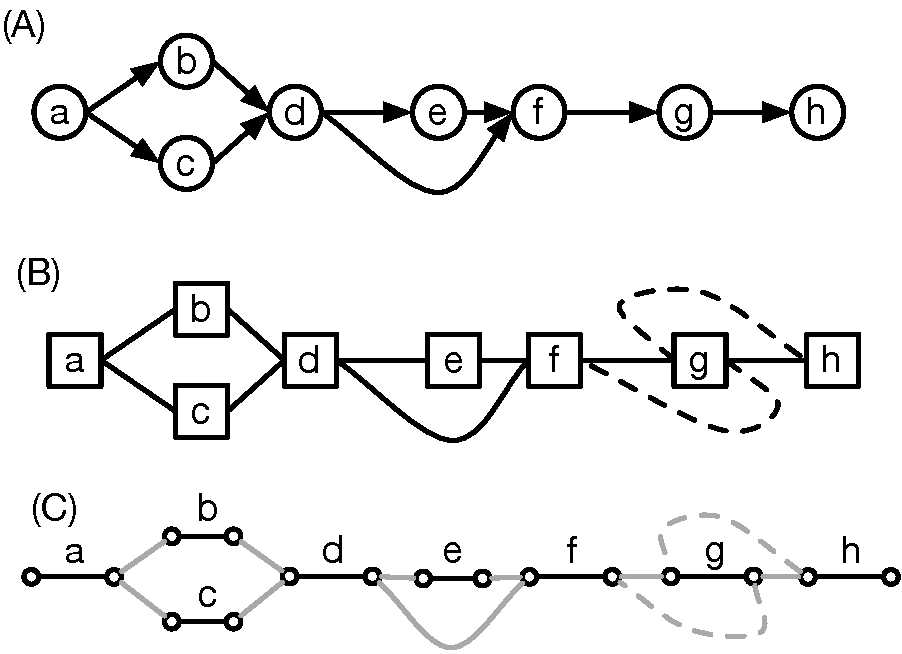
\includegraphics[width=0.7\textwidth]{snarlfigures/fig1.pdf}
\caption{\label{fig:digraphs_and_bigraphs} (A) A digraph.
(B) A bidirected graph. Each node is drawn as a box and the orientation for each edge endpoint is indicated by the connection to either the left or right side of the node. The graph excluding the dotted edges is the equivalent bidirected graph for the digraph in (A); the dotted edges encode an inversion that cannot be expressed in the digraph representation. (C) A biedged graph equivalent to the bidirected graph shown in (B).}
\end{figure}

\subsection{Directed Walks on Biedged and Bidirected Graphs}

%Directed walks on bidirected and biedged graphs
A directed walk on a bidirected graph is a walk that at each visited vertex exits the opposite side to that which it enters. On a biedged graph a directed walk is equivalent to a walk that alternates between black and grey edges. A directed cycle is a closed directed walk that starts and ends either on the same side (e.g.\ a self-loop edge), or on opposites sides of a vertex (in which case the start and end is arbitrary due to symmetry). A bidirected or biedged graph is acyclic if it contains no directed cycles. 

%Relationship of directed walks on digraphs to those on bidirected and biedged graphs
These definitions are a generalization of a directed walk on a digraph. In a bidirected representation of a digraph all edges in a directed walk are all left-to-right or all right-to-left. A directed walk on a general bidirected (or biedged) graph can mix these two types and additionally include edges that do not alternate the orientation of their endpoints (e.g.\ left-right, right-right and left-left edges). 

Given these generalizing relationships, clearly a digraph $\textbf{D}$ is acyclic iff $B(\textbf{D})$ is acyclic. Note that any acyclic biedged graph can also be converted into an equivalent directed acyclic graph (DAG):

\begin{lemma}
For any acyclic biedged graph $B(D)$ there exists an isomorphic biedged graph $B(\textbf{D})$ such that $\textbf{D}$ is a DAG.
\label{lemma_acyclic_biedged_graph_is_dag}
\end{lemma}
\begin{proof}
For each connnected component in $B(D)$, use a depth first search (DFS) beginning at side $x$ to label the sides either `red' or `white':  If $x$ is not already labelled then label $x$ red and $\hat{x}$ white. For each grey edge incident with $\hat{x}$, if the connected side is not labeled, label the connected side red and continue recursively via DFS. In this way all the sides in the connected component containing $x$ will be labeled in a single DFS. If during the recursion the connected side encountered is already labelled then it must be labeled red, else there would exist a directed cycle, a contradiction. Use the labelling to create $B(\textbf{D})$, isomorphic to $B(D)$  but replacing the orientation of the sides so that each side labeled white is a left side and each side labeled red is a right side. All edges in $B(\textbf{D})$ connect a left and a right side.
\end{proof}

\subsection{Superbubbles, Snarls and Ultrabubbles}

%superbubbles

Repeating the definition from \cite{Onodera:2013fo}, any pair of distinct vertices $(x, y)$ in a digraph $\textbf{D}$ is called a \emph{superbubble} (Fig. \ref{fig:super_bubbles_and_complex_bubbles}(A)) if:
\begin{itemize}
\item \emph{reachability}: $y$ is reachable from $x$.
\item \emph{matching}: The set of vertices, $X$, reachable from $x$ without passing through $y$ is equal to the set of vertices from which $y$ is reachable without passing through $x$ (passing through here means to enter and then exit a vertex on the path). 
\item \emph{acyclicity}: The subgraph induced by $X$ is acyclic.
\item \emph{minimality}: No vertex in $X$ other than $y$ forms a pair with $x$ that satisfies the criteria defined above, and similarly for $y$.
\end{itemize}

We call the subgraph induced by $X$ the \emph{superbubble subgraph}.

% Snarls

To generalize superbubbles for biedged graphs we introduce the notion of a snarl, a minimal subgraph in a biedged graph whose vertices are at most 2-black-edge-connected (2-BEC) to the remainder of the graph (two vertices in a biedged graph are $k$-black-edge-connected ($k$-BEC) if it takes the deletion of at least $k$ black edges to disconnect them). In a biedged graph $B(D)$ a pair set of distinct, non-opposite vertices $\{ x, y \}$ are a \emph{snarl} (Fig. \ref{fig:super_bubbles_and_complex_bubbles}(B)) if:
\begin{itemize}
\item \emph{seperable}: The removal of the black edges incident with $x$ and $y$ disconnects the graph, creating a \emph{separated component} $X$ containing $x$ and $y$ and not $\hat{x}$ and $\hat{y}$.
\item \emph{minimality}: No pair of opposites $\{ z, \hat{z} \}$ in $X$ exists such that $\{ x, z \}$ and $\{ y, \hat{z} \}$ fulfils the above criteria.
\end{itemize}

% Ultrabubbles

We call a vertex not incident with a grey edge a \emph{tip} \cite{Zerbino:2008bm}. In a biedged graph $B(D)$ a snarl is an \emph{ultrabubble} if its separated component is acyclic and contains no tips.

The following shows that a superbubble in a digraph is an ultrabubble in the equivalent biedged graph.

\begin{lemma}
For any superbubble $(x, y)$ in a digraph $\textbf{D}$, the pair set $\{ x'=(x, right), y'=(y, left) \}$ is an ultrabubble in $B(\textbf{D})$.
\label{lemma_super_bubble_is_ultra_bubble}
\end{lemma}
\begin{proof}
Let $d$ and $e$ be the black edges incident with $x'$ and $y'$, respectively, and let $X$ be the superbubble subgraph of $(x, y)$.

We start by proving that $\{ x', y' \}$ satisfies the separable criteria. 
As $y$ is reachable from $x$ by definition there exists a directed path in $B(\textbf{D})$ between $x'$ (the right side of $x$) and $y'$ (the left side of $y$) that excludes $d$ and $e$. After the deletion of these black edges $x'$ and $y'$ therefore remain connected.
If the separable criteria is not satisfied the deletion of $d$ and $e$ must therefore not disconnect $x'$ and $y'$ from either or both $\hat{x'}$ and $\hat{y'}$, without loss of generality assume $x'$ (and therefore $y'$) remains connected to $\hat{x'}$. 

If $\hat{x'}$ is on a directed walk from $x'$ that excludes $d$ then the addition of $d$ to this walk defines a directed cycle in $B(\textbf{D})$. As all nodes reachable from $x$ are in the separated component $X$, the existence of this cycle in $B(\textbf{D})$ implies the existence of a corresponding directed cycle in $X$, a contradiction.

If there exists a non-directed walk from $x'$ to $\hat{x'}$ then let $z'$ be the last node on the walk from $x'$ such that the subwalk between $x'$ and $z'$ is a directed walk. By definition, there exists directed walk from $z'$ to $y'$. The next node on the walk from $x'$ to $\hat{x'}$ after $z'$ is, by definition, not reachable from $x'$ but $y'$ must be reachable from this node. This implies a contradiction of the matching criteria for the corresponding nodes in $X$.

We have therefore established that $\{ x', y' \}$ fufills the seperable criteria. We have already established that iff a digraph is acyclic its equivalent biedged graph is acyclic, therefore the seperated component of $\{ x', y' \}$ is acyclic. As every node in $X$ is both reachable from $x$ and on a path from $y$, the separated component clearly contains no tips. 

It remains to prove that $\{ x', y' \}$ fufills the minimality criteria. If $\{ x', y' \}$ do not satisfy the minimality criteria without loss of generality there exists a node $z'$ in the separated component of $\{x', y'\}$ such that $\{x', z' \}$ are separable. It follows that all directed paths from $x'$ to $y'$ that exclude $d$ and $e$ visit $z'$, and for the node $z$ in $\textbf{D}$ contained in $z'$, $(x, z)$ fulfills (clearly) all the superbubble criteria, a contradiction.

\end{proof}


\begin{figure}
\centering
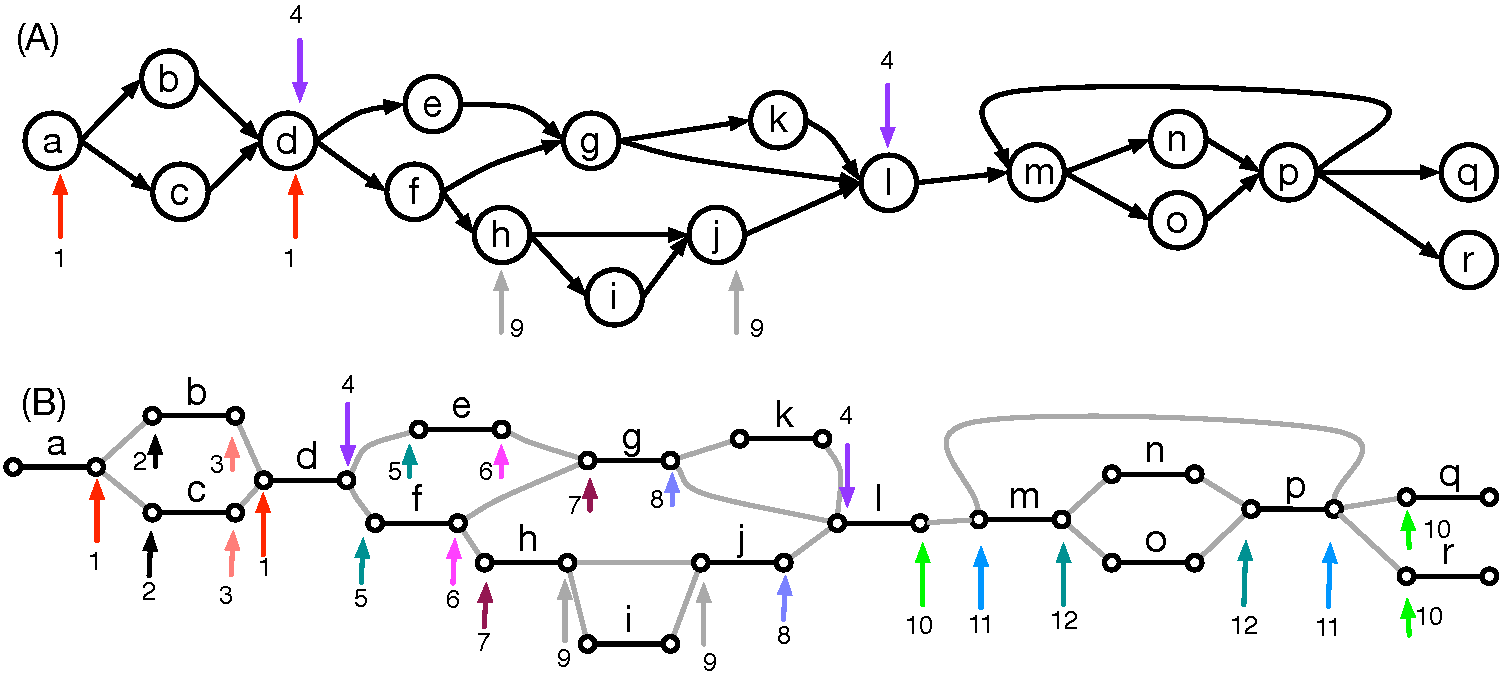
\includegraphics[width=1.0\textwidth]{snarlfigures/fig2.pdf}
\caption{\label{fig:super_bubbles_and_complex_bubbles} (A) Superbubbles in a digraph. The superbubbles are indicated by pairs of numbered arrows, numbered consistently with (B). (B) 
A biedged graph representation of the digraph in (A). The snarls are illustrated by numbered arrows, the ultrabubbles are those numbered 1, 4, 9 and 12. Note, a side incident with a black bridge edge may be in multiple snarls (see snarls numbered 10).}
\end{figure}

%Complex ultrabubbles

\subsection{Cactus Graphs}

%Cactus graph
A cactus graph is a graph in which any two vertices are at most two-edge connected \cite{Harary:1953vba}. In a cactus graph each edge is part of at most one simple cycle, and therefore any two simple cycles intersect at most one vertex. 

%Define vertex merging
For a graph $G = (V_G, E_G)$ let $G' = (V_{G'}, E_{G'})$ be a multigraph created by \emph{merging} subsets of the vertices, such that:
\begin{itemize}
\item$V_{G'}$ is a partition of $V_{G}$,
\item $E_{G'} = \{ \{ a_{G'}(x), a_{G'}(y) \} | \{x, y\} \in E_G \}$ is a multiset.
\end{itemize}
where $a_{G'} : V_G \rightarrow V_{G'}$ is a graph homomorphism that maps each vertex in $V_{G}$ to the set in $V_{G'}$ that contains it. 

%Linking biedged graphs and cactus graphs
Merging all equivalence classes of 3-edge connected (3-EC) vertices in a graph results in a cactus graph \cite{Paten:2011fv}. 

For a  biedged graph $B(D)$ let $C(D)$ be the cactus graph created by first contracting all the grey edges in $B(D)$ then for each equivalence class of 3-EC vertices in the resulting graph merging together the vertices within the equivalence class (Fig. \ref{fig:biedged_graphs_and_cactus_graphs}(A-C)). As with $G'$ and $G$, $V_{C(D)}$ is a partition of the vertices of $V_{B(D)}$, and $E_{C(D)} = \{ \{ a_{C(D)}(x), a_{C(D)}(y) \} | \{x, y\} \in E_{B(D)} \}$ is a multiset. 

%Notation 
For a vertex $x \in V_{B(D)}$ we call $a_{C(D)}(x)$ its \emph{projection} (in $C(D)$). Similarly for a set of vertices $X \subset V_{B(D)}$ we call $\{ a_{C(D)}(x) | x \in X \}$ the projection of $X$ (in $C(D)$). Let $b_{C(D)}(x) = \{ a_{C(D)}(x), a_{C(D)}(\hat{x}) \}$, which is the projection of the black edge incident with $x$ in $C(D)$.

%Linking B(D) and C(D)
Appendix 1 gives lemmas that make explicit the relationship between the edge connectivity of vertices in $B(D)$ and $C(D)$, and which we use to prove the relationship between the snarls of $B(D)$ and $C(D)$. 

\begin{figure}
\centering
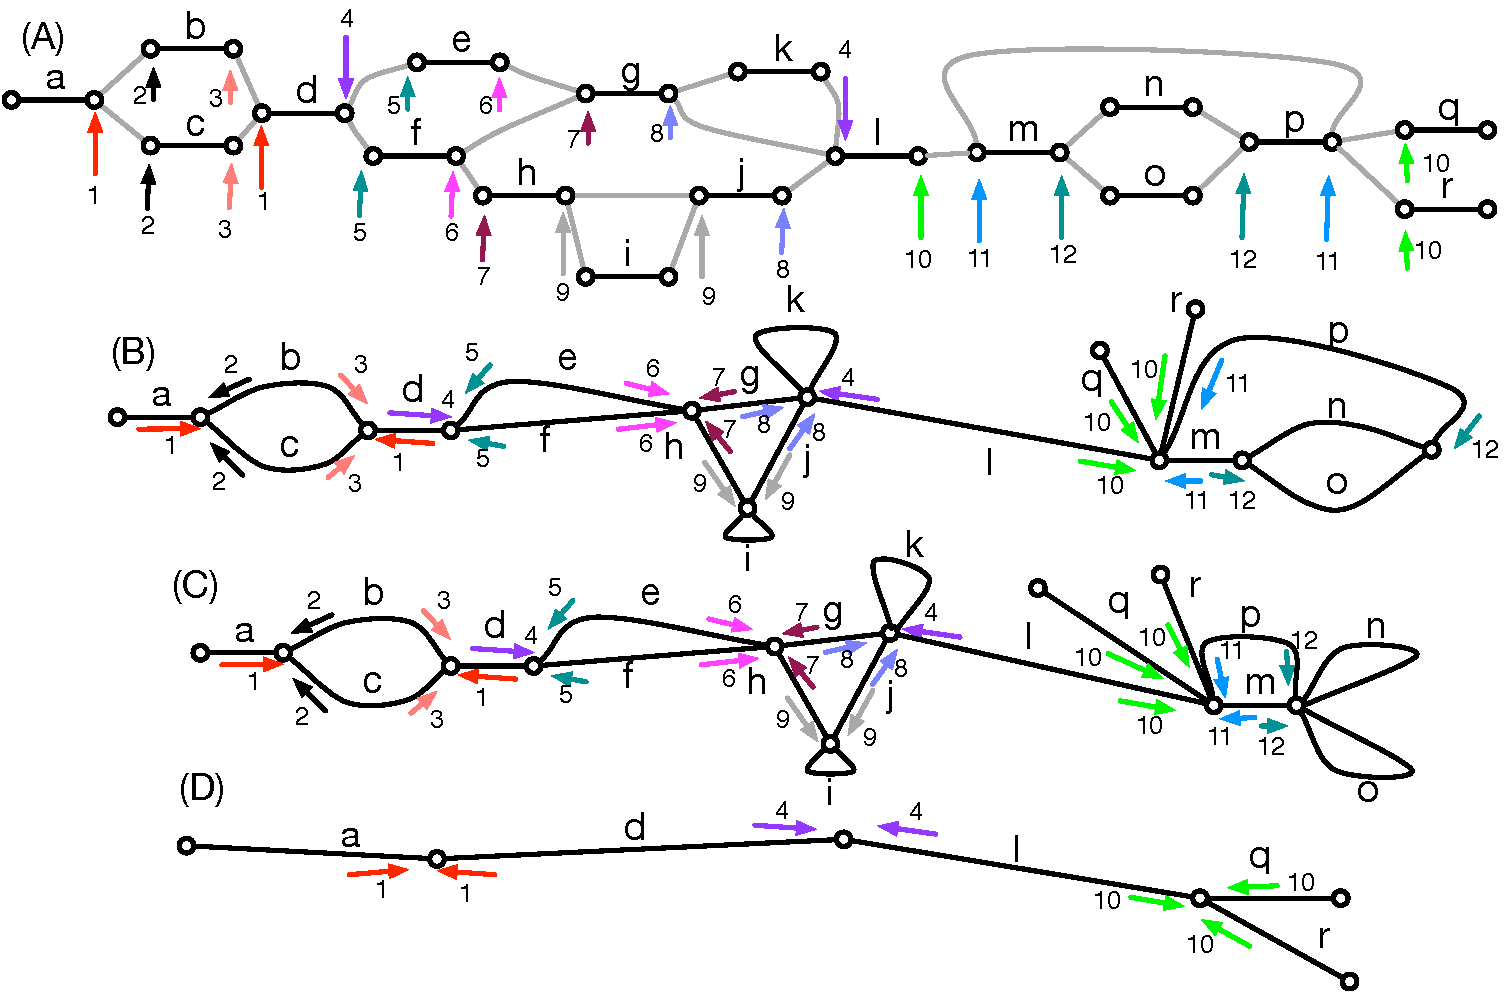
\includegraphics[width=0.9\textwidth]{snarlfigures/fig3.pdf}
\caption{\label{fig:biedged_graphs_and_cactus_graphs} (A) A biedged graph $B(D)$ with the snarls indicated by pairs of numbered arrows. (B) The graph in (A) after contracting the grey edges. (C) The cactus graph $C(D)$ for $B(D)$, constructed by merging the vertices in each 3-EC in (B). (D) The bridge forest $D(D)$, constructed by constracting the edges in simple cycles in (C). }
%(E) A net graph for the number 4 bridge pair in (A). The projection of chain pairs in $B(D)$ to the other graphs is shown using the numbered arrows, with the arrows drawn along the projecting black edge incident with the projected vertex.}
\end{figure}

\subsection{Snarls and Cacti}

%Chain pair and cyclic chains
A pair set of distinct vertices $\{ x, y \}$ in $B(D)$ are a \emph{chain pair} if they project to the same vertex in $C(D)$ and their incident black edges project to the same simple cycle in $C(D)$ (e.g.\ pairs of arrows in simple cycles  in Fig. \ref{fig:biedged_graphs_and_cactus_graphs}(C)). A cyclic sequence of chain pairs within the same simple cycle in $C(D)$ and ordered according to the ordering of this simple cycle is a \emph{(cyclic) chain}. Contiguous chain pairs in a chain share two opposite sides of a black edge in $B(D)$.

%Bridge forest
For a cactus graph $C(D)$, the graph $D(D)$ resulting from contracting all the edges in simple cycles in $C(D)$ is a called a \emph{bridge forest} (Fig. \ref{fig:biedged_graphs_and_cactus_graphs}(D)).

%Bridge pair and acyclic chains
A pair set of distinct vertices $\{ x, y \}$ in $B(D)$ are a \emph{bridge pair} if they project to the same vertex in $D(D)$  and both their incident black edges are bridges (e.g.\ pairs of arrows numbered 1 and 2 in Fig. \ref{fig:biedged_graphs_and_cactus_graphs}(D)). A maximum sequence of bridge pairs within $D(D)$ connected by incident nodes with degree two is an \emph{(acyclic) chain}. As with chain pairs, contiguous bridge pairs in a chain share two opposite sides of a black (bridge) edge in $B(D)$.


\begin{theorem}
The set of snarls in $B(D)$ is equal to the union of chain pairs and bridge pairs.
\label{theorem_chain_and_bridge_pair_bijection_complex_bubbles}
\end{theorem}
\begin{proof}
Follows from Lemmas 10 and 11 given in Appendix 2.
\end{proof}

Given Theorem \ref{theorem_chain_and_bridge_pair_bijection_complex_bubbles} to calculate the set of snarls for a given biedged graph it is sufficient to calculate the cactus graph to give the set of snarls that map to chain pairs and the bridge forest to calculate the set of snarls that map to bridge pairs. Constructing a cactus graph of the type described for a biedged graph is linear in the size of the biedged graph (using the algorithm described in \cite{Paten:2011fv}), and clearly the cost of then calculating the bridge forest from the cactus graph is similarly linear. The number of chain pairs is clearly linear in the size of the biedged graph, however, the number of bridge pairs is potentially quadratic in the number of bridge pairs, so enumerating these latter snarls has potentially worst case quadratic cost in terms of the size of the biedged graph. Below we consider ways to prune the set of snarls by using their natural nesting relationships to create a hierarchy of snarls that is at most linear in the size of the biedged graph. 

\subsection{Compatible Snarl Families}

One particularly attractive feature of superbubbles is that they have nested containment relationships. That is, superbubbles have subgraphs that are either strictly nested or disjoint. Accordingly, a digraph is partitioned into a set of top level superbubble subgraphs and other graph members not contained in a superbubble subgraph, and each top level superbubble component then contains one or more child superbubbles, forming a tree structure. The situation is more complex for snarls. The separated component of snarls can overlap (Fig. \ref{fig:overlapping_snarls}) such that each partially contains the other. To create a properly nested hierarchy of snarls it is therefore necessary to exclude some snarls.

\begin{figure}
\centering
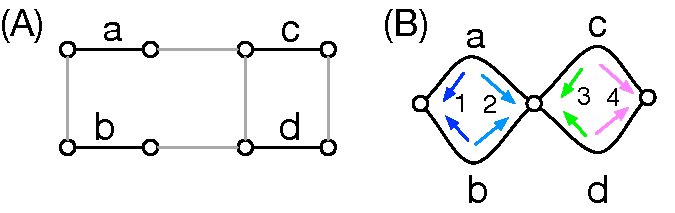
\includegraphics[width=0.4\textwidth]{snarlfigures/fig4.pdf}
\caption{\label{fig:overlapping_snarls} Overlapping snarls. (A) A bidirected graph, its corresponding (B) cactus graph. The snarl numbered 2 contains the snarl numbered 4, similarly the snarl numbered 3 contains the snarl numbered 1. The snarls numbered 2 and 3 overlap.}
\end{figure}

We will call a family of snarls \textit{compatible} if all pairs of distinct snarls in the family have snarl subgraphs that are either disjoint or nested. A compatible family of snarls has a nesting structure that is a forest, similar to superbubbles. The following theorem provides a sufficient condition for constructing such a family in many bidirected graphs.

\begin{theorem}
	In a connected biedged graph with at least one black bridge edge, the family of snarls whose subgraphs have no black bridge edges is compatible.
	\label{theorem_no_bridges_is_compatible}
\end{theorem}

\noindent In addition, the next theorem shows that this family of snarls is a generalization of ultrabubbles.

\begin{theorem}
	No ultrabubble contains a black bridge edge in its subgraph.
	\label{theorem_ultrabubbles_have_no_bridges}
\end{theorem}

\noindent Proofs of these theorems are included in Appendix 3.	

The bridge edge condition can also be used to construct a compatible family of snarls in a graph with no black bridge edges. To do so, we break one black edge into two tips. Each of these tips is then a bridge edge, so the family of snarls we construct from the modified graph is compatible. However, the family of snarls we obtain will depend on our choice of a black edge to break.  Heuristically, an edge corresponding to a highly conserved genomic element should be chosen, since by construction it will not occur in any snarl's subgraph.

Given a snarl decomposition, the following algorithm will filter them down to the compatible family we have described:

\begin{itemize}
	\item Iterate over the black bridge edges of the graph (i.e.\ the edges of $D(D)$)
	\item For a bridge edge $(u, \hat u)$, if either $u$ or $\hat u$ is the boundary of a snarl, mark that snarl as not containing $(u, \hat u)$.
	\item Initialize a queue with $u$ and $\hat u$, and traverse outward in breadth-first order, ignoring restrictions on directed biedged walks. 
	\item Upon reaching a node $x$ that is a boundary for a snarl $\{x,y\}$, if neither $y$, $\hat x$, nor $\hat y$ have been traversed, mark the snarl as containing $(u, \hat u)$.
 	\item Upon reaching a node $\hat x$ whose opposite is boundary for a snarl $\{x,y\}$, if neither $\hat y$, $x$, nor $y$ has been traversed, mark the snarl as not containing $(u, \hat u)$.
 	\item After completing every traversal, retain only snarls that were never marked as containing a black bridge edge.
\end{itemize}

The validity of this algorithm is proven by Lemma \ref{lemma_shortest_path_determines_subgraph_membership}. Naively, this algorithm requires $O(|E_{B(D)}|(|V_{B(D)}| + |E_{B(D)}|))$ time for the traversals, and $O(|V_{B(D)}|^2)$ to mark all snarls. However, we can implement optimizations that improve on this behavior. First, we can also stop the BFS traversals whenever they encounter a bridge edge. Lemmas \ref{lemma_snarls_across_bridges_are_redundant} and \ref{lemma_snarl_on_bridge_is_in_one_component} demonstrate that the portion of the BFS traversal after a bridge edge is redundant. This reduces the time required for the traversal to $O(M(|V_{B(D)}| + |E_{B(D)}|))$, where $M = \max_{v \in V_{D(D)}} \deg v$. In general, $M = O(|E_{B(D)}|)$, so this does not improve over the worst case asymptotic bound. However, in many practical cases $M$ is approximately constant. 

 We can also reduce the total number of snarls we need to filter by neglecting to produce some snarls a priori. The quadratic bound on the number snarls is due to the fact that there is a bridge pair for all pairs of edges incident on a  node in $D(D)$. However, Lemma \ref{lemma_shared_boundary_implies_bridge_edge} shows that none of these bridge pairs will pass the filter. Accordingly, we can reduce the set of snarls we consider to only chain pairs and bridge pairs that project to nodes of degree 2 in $D(D)$, which we call \emph{simple} bridge pairs. This reduces the total number of snarls to $O(|V_{B(D)}|)$.

\subsection{Ultrabubbles and Cacti}

% Testing acyclicity using the cactus

Given Theorem \ref{theorem_chain_and_bridge_pair_bijection_complex_bubbles}, to determine the ultrabubbles in $B(D)$ it is sufficient to check for each chain and bridge pair if the separated component is acyclic and contains no tips. 

Using Theorem \ref{theorem_ultrabubbles_have_no_bridges} we can restrict the search to snarls whose separated component does not contain a black bridge edge. This implies that we need only consider bridge pairs whose projection in $D(D)$ is a node whose degree is two, we call such bridge pairs \emph{simple}. The number of simple bridge pairs must be less than the cardinality of $D(D)$, and therefore the total number of chain pairs and simple bridge pairs is less than or equal to $|E_{B(D)}|$.  Using $D(D)$ and $C(D)$, which both can be constructed in $O(|E_{B(D)}| + |V_{B(D)}|)$ time, we can clearly enumerate the set of simple chain pairs and bridge pairs in $O(|E_{B(D)}| + |V_{B(D)}|)$ time. 

A simple algorithm to find the set of ultrabubbles enumerates all chain pairs and simple bridge pairs and checks for each the acyclicity and tipless requirement using a depth first search, and is therefore worst case $O((|E_{B(D)}| + |V_{B(D)}|)^2)$ time.

\section{Discussion and Conclusion}

% Discuss open question - how to classify snarls that are not ultrabubbles. 

We have presented a partial decomposition of a bidirected graph into a set of nested snarls and ultrabubbles. We believe this solves an important problem in using graphs for representing arbitrary genetic variations by defining a decomposition that determines sites and alleles. 

As the decomposition is only partial, not all elements in a graph will necessarily fit into one of the ultrabubbles. However, we demonstrate that for an existing large library of variation (1000 Genomes) the large majority of sites are either invariant or described by simple, top-level ultrabubbles. 

For bases outside of these easy sites it is possible to imagine further subclassification. For example, classifying snarls that contain tips but are acyclic might define a useful class of subgraph common in some subproblems (e.g.\ sequence assembly). Some structures representing dense or overlapping collections of sequence polymorphisms, insertions and deletions cannot be fully described using nested ultrabubbles. We have previously shown that a generalization of the separability criterion for ultrabubbles can describe sites in these cases. \cite{Rosen2017}. Similarly, characteristic structures representing genomic phenomena, such as inversions and translocations, are imaginable. Beyond our initial investigation, a more thorough evaluation of how much of a graph fits within a snarl, ultrabubble, or one of these more complex structures would be a useful exercise. We propose that the compatible family of snarls we constructed provides one path forward in this endeavor.

% Discuss strategy to heuristically make ultrabubbles

We can also envision that the nesting structure of snarls could play a powerful role in decomposing genotyping problems. Nested graph structures often arise from nested indels and substitutions. 
%This perspective reframes the genotyping problem as the problem of establishing a consistent traversal of each snarl's net graph.

%\begin{figure}}
%\centering
%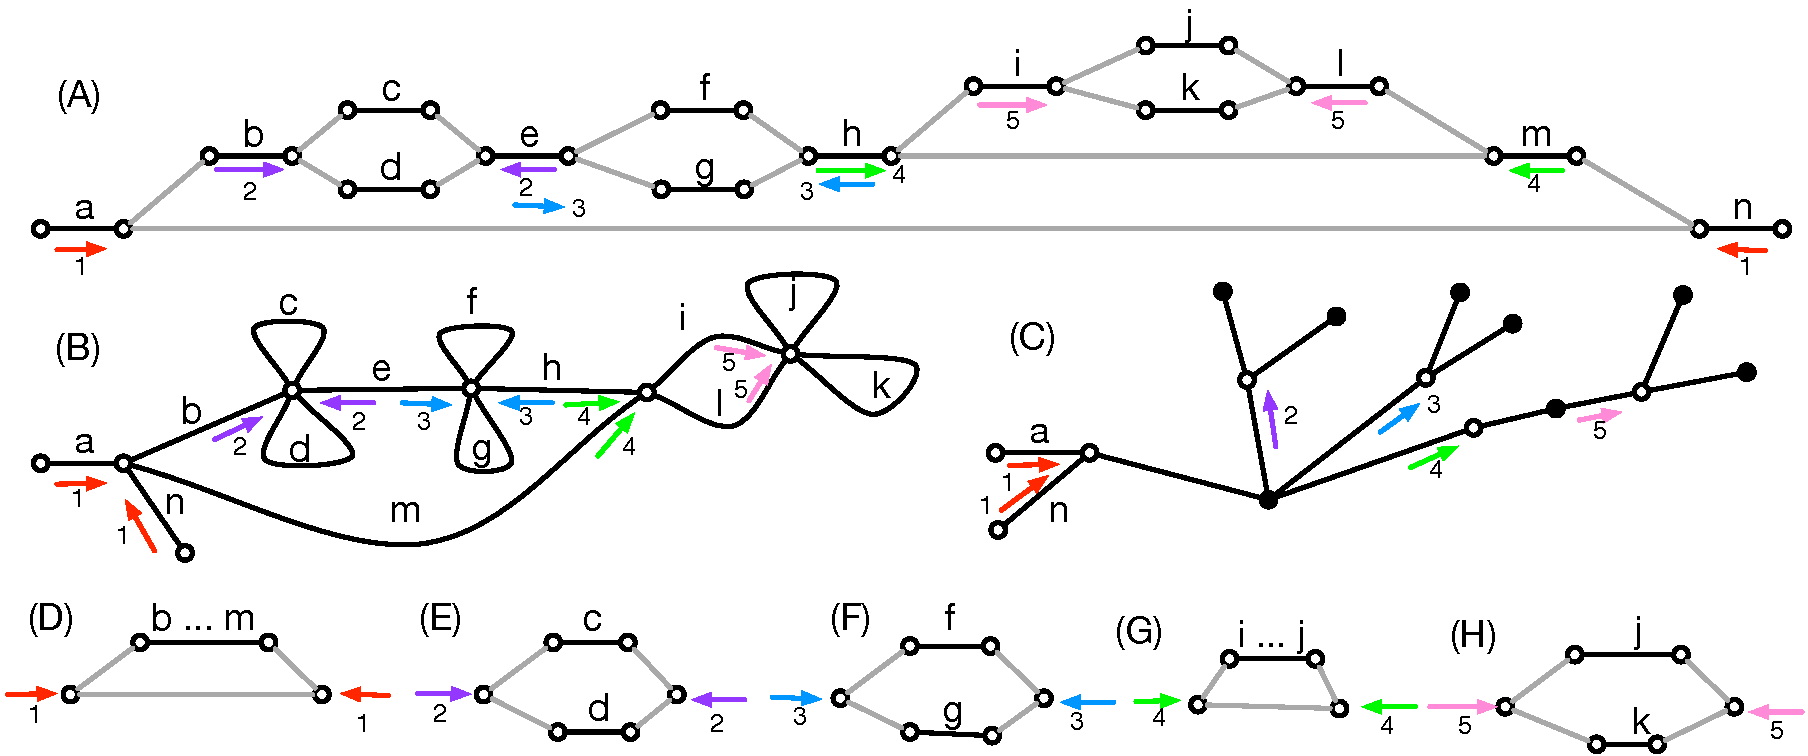
\includegraphics[width=1.0\textwidth]{fig5.pdf}
%\caption{\label{fig:nested_ultra_bubbles} (A) A biedged graph $B(D)$ with nested ultrabubbles indicated by pairs of numbered arrows. (B) $C(D)$ for $B(D)$. (C) $T(D)$ for $B(D)$. (D-H) The net graphs for the ultrabubbles in $B(D)$.}
%\end{figure}

In the context of assembly, various error correction algorithms have been proposed to remove graph elements and reduce the complexity of the graph. This increases the fraction of the graph that is contained within an ultrabubble structure. We foresee the cactus graph structure providing a useful basis for exploring such algorithms. 

\section{Acknowledgements}

This work was supported by the National Human Genome Research Institute of the National Institutes of Health under
Award Number 5U54HG007990 and grants from the W.M. Keck foundation and the Simons Foundation. This work benefitted from numerous conversations with David Haussler and Daniel Zerbino.

\chapter{Walk-preserving transformation of overlapped sequence graphs into blunt sequence graphs}
\label{chapter:bluntifier}

\section{Preamble}

This chapter consists of the full text of a paper ``Walk-preserving transformation of overlapped sequence graphs into blunt sequence graphs with GetBlunted'', which will be presented at the 2021 meeting of Computability in Europe. I share primary authorship for this paper with Ryan Lorig-Roach. I am responsible for designing and partially implementing the algorithms, as well as writing the majority of the paper. Ryan Lorig-Roach also partially implemented the algorithm, and Melissa M. Meredith performed the experimental comparison to comparable algorithms.

\section{Introduction}

% sequence graphs have long history in assembly
Genome assembly is the process of determining a sample's full genome sequence from the error-prone, fragmentary sequences produced by DNA sequencing technologies.
Sequence graphs have a long history of use in this field \cite{myers1995toward,pevzner2001eulerian,myers2005fragment}.
In these graphs, nodes are labeled with sequences derived from sequencing data, and edges indicate overlaps between observed sequences, which may in turn indicate adjacency in the sample's genome (\figref{seqgraphs}A).
The sample genome then corresponds to some walk through graph.
% description of de bruijn and overlap graphs / string graphs
There are several specific sequence graph articulations in wide use, including de Bruijn graphs, overlap graphs, and string graphs.
They each present computational and informational trade-offs that make them better suited to certain configurations of sequencing technologies and genome complexity.

The common topological features of genome assembly graphs are driven primarily by the repetitiveness of the underlying genomes.
In many species, a large fraction of the genome consists of repeats (for instance, more than 50\% of the human genome \cite{haubold2006repetitive}).
Because all copies of a repeat are highly similar to each other, the corresponding nodes in the sequence graph frequently overlap each other.
In contrast, the unique regions of the genome have few erroneous overlaps.
These two factors tend to create graphs that consist of long non-branching paths (corresponding to the unique regions), which meet in a densely tangled core with a complicated topology (corresponding to the repeats).

% growth of sequence graphs as formalism in pangenomics
Recently, sequence graphs have also emerged into prominence in the growing field of pangenomics, which seeks to analyze the full genomes of many individuals from the same species \cite{computational2018computational}.
In pangenomics, sequence graphs are used to represent genomic variation between individual haplotypes.
Sequences in the graph furcate and rejoin around sites of variation so that each individual genome corresponds to a walk through the graph (\figref{seqgraphs}B).
% state of the art practical tools and formal algorithms research
The growth of pangenomics has fueled major advances in both formal algorithms research \cite{rautiainen2017aligning,jain2020complexity} and practical genomics tools \cite{garrison2018variation,rautiainen2020graphaligner}.

Pangenome graphs have much simpler topologies than genome assembly graphs.
Having fuller knowledge of the constituent genomes makes it possible to distinguish different copies of a repeat.
Thus, pangenome graphs tend to be mostly non-branching, much like the portions of assembly graphs that correspond to unique sequences in the genome.
Moreover, most of the branching in pangenome graphs consists of localized bubble-like motifs.
In contrast to assembly graphs, pangenome graphs have few if any cycles.

\begin{figure}
\begin{center}
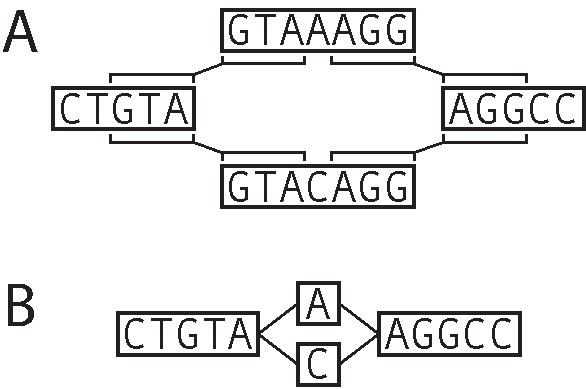
\includegraphics[width=.5\textwidth]{bluntfigures/overlap_vs_blunt.pdf}
\caption{\textbf{A}: An overlapped sequence graph. \textbf{B}: A blunt sequence graph.} \label{fig:seqgraphs}
\end{center}
\end{figure}

% focus on blunt ended graphs in this research
Intuitively, the shared basis in sequence graphs should permit the advances in pangenomics to spill over into genome assembly.
However, such cross-pollination is stymied by a small difference in the graph formalisms.
The edges in assembly graphs indicate sequence overlaps, which are necessary because of the uncertain adjacencies in the underlying genome.
In pangenome graphs, the underlying genomes are known, and the edges are \emph{blunt} in that they indicate direct adjacency with no overlap.
% translation from blunt to overlap is trivial, but reverse is difficult
Blunt sequence graphs can be trivially converted into overlap graphs (with overlaps of length 0), but the reverse requires nontrivial merging operations between the overlapping sequences.
% result is that tools developed for pangenomics remain siloed despite potential uses in genome assembly
As a result, methods have remained siloed within pangenomics despite potential uses in genome assembly.

In this work, we present a method to transform an overlapped sequence graph into a blunt sequence graph. 
We state the formal guarantees of our formulation and discuss their computational complexity. 
We then present an algorithm and compare its results to similar methods.

\section{Problem statement}

% our goal is to produce a translation of overlap to blunt with two properties
% - all walks through the graph are preserved
% - no walks through the blunt graph are impossible in the overlap graph
In transforming an overlapped sequence graph to a blunt one, we seek to provide two guarantees:
\begin{enumerate}
    \item All walks in the overlapped graph are preserved in the blunt graph.
    \item Every walk in the blunt graph corresponds to some walk in the overlapped graph.
\end{enumerate}
% z motif creates problems for property 2, must duplicate
These two properties prohibit the intuitive solution of transitively merging all overlapped sequences.
Doing so can result in walks that are not present in the overlapped graph, because walks can transition between nodes that are not connected by an edge via the transitively merged sequences (\figref{transitive}).
Because overlapped sequences cannot be fully merged, it is necessary to retain multiple copies of some sequences in the blunt graph.
% duplication increases alignment uncertainty, we attempt minimize duplication
However, excessive duplication can create problems for downstream analysis, for instance by increasing alignment uncertainty.
Thus, we add one further criterion to the above formulation:
\begin{enumerate}
  \setcounter{enumi}{2}
  \item Minimize the amount of duplicated sequence.
\end{enumerate}

\begin{figure}
\begin{center}
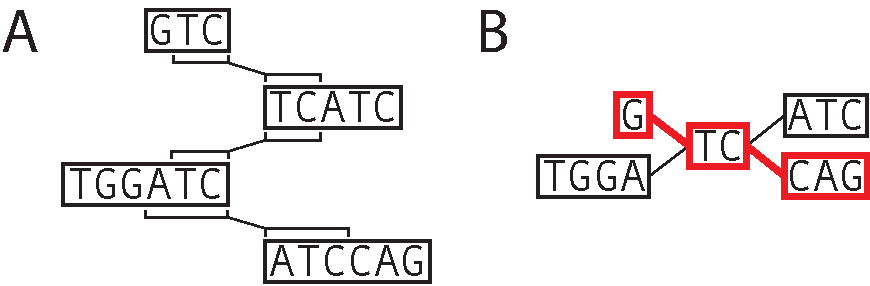
\includegraphics[width=.8\textwidth]{bluntfigures/transitive_collapse.pdf}
\caption{\textbf{A}: An overlapped sequence graph, and \textbf{B}: the blunt sequence graph that results from transitively merging its overlaps. The highlighted walk in the blunt graph does not correspond to any walk in the original overlapped graph.} \label{fig:transitive}
\end{center}
\end{figure}

\section{Notation}

An overlapped sequence graph consists of a set of sequences $S$ and a set of overlaps $O \subset (S \times \{+,-\} \times S \times \{+,-\})$. 
In this notation, the symbols $+$ and $-$ indicate whether the overlap involves a prefix or suffix (collectively \emph{affix}) of the sequence.
This makes the overlapped graph a bidirected graph. 
%Additionally, each overlap is labeled with its length. 

In a bidirected graph, a \emph{walk} consists of a sequence of nodes $s_1s_2\ldots s_N$, $s_i \in S$ such that 1) each pair of subsequent nodes is connected by an overlap and 2) if $s_{i-1}$ and $s_i$ are connected by an overlap on $s_i$'s prefix, then $s_i$ and $s_{i+1}$ are a connected by an overlap on $s_i$'s suffix (or vice versa).
In the case that a walk traverses a node $s \in S$ from suffix to prefix, we interpret the sequence as its \emph{reverse complement}, which is the sequence of the antiparallel strand of the DNA molecule. 

Finally, an \emph{adjacency component} is a collection of affixes (in $S \times \{+,-\}$) that can reach each other via a sequence of adjacent overlaps in $O$ (\figref{adjacency}).
This sequence need not form a valid bidirected walk.

\begin{figure}
\begin{center}
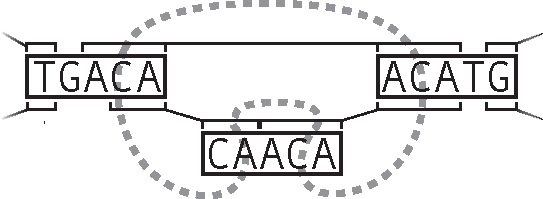
\includegraphics[width=.6\textwidth]{bluntfigures/adjacency_component_3.pdf}
\caption{An adjacency component in a larger sequence graph. Each of the indicated affixes can reach the others by a sequence of overlaps.} \label{fig:adjacency}
\end{center}
\end{figure}

\section{Methods}

% minimizing duplication requires minimizing number of transitive merges
To minimize the amount of duplicated sequence, overlapped sequences must be merged. 
However, we have already mentioned that our criteria prohibit transitively merging all overlaps.
We must then minimize the total number of groups within which overlaps are merged transitively, which coincides with the number of times the sequences need to be duplicated.

% safe merges need to be part of a biclique
Consider a group of overlaps that contains $(s_1, s_2, +, -)$ and $(t_1, t_2, +, -)$.
For merging to not introduce any walks that are not in the overlapped graph, the overlaps $(s_1, t_2, +, -)$ and $(t_1, s_2, +, -)$ must also be overlaps in $O$.
Extending this logic, the entire group of overlaps must be contained within a \emph{biclique} subgraph of the adjacency component: two sets of affixes $B_1$ and $B_2$ such that every affix in $B_1$ is connected to every affix in $B_2$ by an overlap.
Thus, we can minimize the number of duplicated sequences by minimizing the number of bicliques needed to cover every overlap edge.

% because adjacency components are usually bipartite (odd cycles require palindromic sequence) and overlaps are approximately transitive, most cases are exactly computable with domino-free algorithm
The problem of covering edges with the minimum number of bicliques is known as \emph{biclique cover} (\figref{biclique}), and it is known to be NP-hard \cite{orlin1977contentment}.
However, there are domain-specific features of overlapped sequence graphs that often make it tractable to solve large portions of the graph optimally.

\begin{figure}
\begin{center}
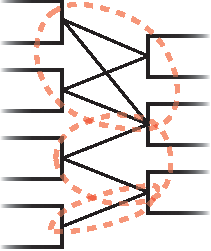
\includegraphics[width=.2\textwidth]{bluntfigures/biclique_cover.pdf}
\caption{A biclique cover of an adjacency component with three bicliques.} \label{fig:biclique}
\end{center}
\end{figure}

First, many adjacency components are bipartite.
Consider the case that an adjacency component is not bipartite, in which case there is cycle of overlaps between affixes with odd parity.
Each overlap indicates high sequence similarity, so an odd cycle means that each sequence is similar to itself, reverse complemented an odd number of times.
Such sequences are called DNA palindromes, and they do exist in nature.
However, they comprise a small fraction of most real genomes.

Second, most adjacency components are \emph{domino-free}. 
This property refers to the absence of a particular induced subgraph, the \emph{domino} (\figref{domino}).
A sufficient condition to prohibit dominoes is for overlapping to be a transitive property.
That is, whenever sequence $s_1$ overlaps sequences $t_1$ and $t_2$, and sequence $s_2$ overlaps $t_1$, then $s_2$ also overlaps $t_2$.
In reality, this is not always the case.
However, it is very often the case, since overlaps indicate sequence similarity, and similarity is approximately transitive.
    
\begin{figure}
\begin{center}
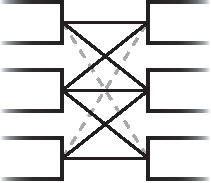
\includegraphics[width=.2\textwidth]{bluntfigures/domino.pdf}
\caption{The domino graph. If either of the dotted edges are present, the induced subgraph is not a domino.} \label{fig:domino}
\end{center}
\end{figure}

These features guided the design of the following algorithm. If an adjacency component is bipartite and domino-free, we compute the biclique cover in polynomial time with the algorithm of Amilhastre, Vilaren, and Janssen \cite{amilhastre1998complexity}.
% remaining cases are handled by combination of maximum bipartite subgraph (max-cut) and heuristic reductions from Ene
When an adjacency component is bipartite but not domino-free, we instead use the dual graph reduction algorithm of Ene, et al. \cite{ene2008fast}, followed by their lattice-based post-processing if the algorithm does not identify the optimal solution.
Finally, if an adjacency component is not bipartite, we first reduce it to the bipartite case by computing an approximate solution to the maximum bipartite subgraph problem using the algorithm of Bylka, Idzik, and Tuza \cite{bylka1999maximum}. 
The maximum bipartite subgraph problem is equivalent to max cut, which is also NP-hard \cite{karp1972reducibility}.
This process is repeated recursively on the edges that are not included in the bipartite subgraph.

% bicliques are aligned with partial order alignment
The amount of duplicated sequence is also affected by the manner in which sequences are merged among the overlaps of a biclique.
To minimize duplicated sequence, we must maximize matches in the alignment between the overlapped sequences.
This is the multiple sequence alignment problem, which is NP-hard.
We use the partial order alignment algorithm to approximate the optimal multiple sequence alignment \cite{lee2002multiple}.
Partial order alignment also has the advantage that the alignment is expressed as a blunt sequence graph, which can be directly incorporated in the full blunt graph.

\section{Implementation}

% based on the GFA format
We have implemented the algorithm described here as a genomics tool called GetBlunted.
GetBlunted takes as input a GFA file (a common interchange format for sequence graphs \cite{gfaspec}) and outputs a GFA containing a blunt graph.
% outputs translation table so that operations in the blunt graph can be translated back to the overlap graph
In addition, it provides a translation table from sequences in the output to sequences in the input, which can be used to translate analyses performed on the blunt graph into analyses on the overlapped graph.
% implemented in C++ using libraries that we cite
The implementation is written entirely in C++, and it use several auxiliary libraries: GFAKludge is used for manipulating GFA files \cite{dawson2019gfakluge}, libbdsg is used to represent sequence graphs \cite{eizenga2020efficient}, and SPOA is used for partial order alignment \cite{vaser2017fast}.

\section{Results}

%Memory
%Speed

We compared the performance of GetBlunted to two other tools that transform overlapped sequence graphs into blunt graphs: the gimbricate/seqwish \cite{garrison_ekggimbricate_2020,garrison_ekgseqwish_2021} pipeline and Stark \cite{nikaein_hnikaeinstark_2021}. 
These are, to our knowledge, the only other such tools besides GetBlunted.
However, they are not completely comparable.
Neither tool provides the guarantees that GetBlunted does for preserving the walk space of the graph.
In addition, Stark only works with de Bruijn graphs, a restricted subset of overlap graphs in which all overlaps are exact matches of a uniform length.

We profiled speed and memory usage on three assembly graphs.
The first two are assembly graphs produced by the Shasta assembler \cite{shafin_nanopore_2020} for the haploid human cell line CHM13 and for human sample HG002.
Both of these were built using Oxford Nanopore reads\footnote{Publicly available at \url{https://s3-us-west-2.amazonaws.com/miten-hg002/index.html?prefix=guppy\_3.6.0/}}.
The last graph is a de Bruijn graph of Pacific Biosciences HiFi reads of an \textit{Escherichia coli} strain (SRR10382245), which was constructed using jumboDB \cite{bankevich_assembling_2020}.

All of the bluntifying tools were run on a single core of a c5.9xlarge AWS instance with an Intel Xeon Scalable Processor.
Memory usage and compute time were measured with the Unix time tool.
The results of the profiling are presented in Table \ref{table:1}.
GetBlunted is over 1000 times faster than and comparably memory-intensive to the gimbricate/seqwish pipeline. 
For de Bruijn graphs, Stark is faster than either tool, although this performance comes at the cost of limited generality.

%Parsimony
%Guarantees walk space, works on general overlap graphs

\begin{table}[h!]
\ssp
\begin{center}
\begin{tabular}{ ||p{2cm}|p{3cm}|p{2.75cm}|p{2cm}|| }
%|m{3cm}|m{3cm}|m{3cm}|m{3cm}|m{3cm}| } 
\hline
Assembly & Bluntification Tool & Run Time (min) & RAM (GB) \\
\hline
\multirow{2}{2cm}{HG002 Shasta} & GetBlunted & 0.35 & 9 \\ 
&  gimbricate/seqwish  & 917.5 &  6 \\ 
\hline
\multirow{2}{2cm}{CHM13 Shasta} & GetBlunted & 0.38 & 4 \\ 
&  gimbricate/seqwish  & 314.6 &  6 \\ 
\hline
\multirow{3}{2cm}{\emph{E. coli} de Bruijn} & GetBlunted & 8.36 & 26 \\ 
&  gimbricate/seqwish  & 10.74 &  4 \\
& Stark & 0.65 & 3\\
\hline
\end{tabular}
\end{center}
\caption{Table of speed and memory usage of bluntifing tools run on a single core of an AWS server.}
\label{table:1}
\end{table}

\section{Discussion}

In this work, we described an algorithm and software tool, GetBlunted, which transforms overlapped sequence graphs into blunt sequence graphs. 
This provides a route for sequence graph methods developed for pangenomics to be applied to sequence graphs in genome assembly.
In both fields, walks through the sequence graph are of primary importance.
In genome assembly, some walk through the graph corresponds to the sample genome.
In pangenomics, the genomes used to construct the pangenome each correspond to a walk through the graph.
GetBlunted provides attractive guarantees that it faithfully preserves the walk space of the input while also producing parsimonious output.
Other comparable methods either do not provide these guarantees or only provide them in limited cases.
In addition, GetBlunted is (except in the case of de Bruijn graphs) faster than alternatives that do not provide these guarantees, and it has resource requirements that are easily achievable in any computational environment that is used for genome assembly.
In the future, GetBlunted could serve as an step in genome assembly pipelines to improve the quality of their overlap graphs.
It could also facilitate direct analyses of assembly graphs in metagenomics applications.

\part{Discussion}

\chapter{Discussion}
\label{chapter:discussion}

%In this dissertation, I have described some of my contributions to graph-based methods in pangenomics. Some of these 

For many years, progress in pangenomics was hampered by ascertainment bias in genomic variation assays. In order to comprehensively identify minor alleles, sequencing projects needed to be carried out at population scale. The only genome inference technologies that were economical at this scale were genotype arrays and NGS variant calling. Accordingly, scientific knowledge of variation shared these assays' biases. The ascertained variants were disproportionately small and disproportionately located in high-complexity, unique regions of the genome. Almost by definition, these are the variants that were least likely to have been substantially impacted by reference bias to begin with.

This situation is now beginning to change. Advancements in long read assembly methods are shining a light on previously hidden regions of the genome. This can be seen in the first complete human genome assembly by the T2T Consortium\cite{nurk2021complete} or in the intensive characterization of structural variation by the Human Genome Structural Variation Consortium (HGSVC)\cite{chaisson2019multi,ebert2021haplotype}. The Human Pangenome Reference Consortium (HPRC) is currently engaged in a similar assembly effort\cite{genomeweb2021hprc}. These data resources are already being used in pangenomics applications to genotype structural variation with NGS data\cite{ebler2020pangenome,siren2020genotyping}, a poster child for genomics tasks that were previously frustrated by severe reference bias.

The research presented in this dissertation sits somewhere on the threshold between these two periods of pangenomics. In chapter \ref{chapter:snarls}, I helped establish foundational theory for pangenome graphs. Chapters \ref{chapter:handle} and \ref{chapter:autoindex} detail engineering efforts that underlie the recent emergence of practical and usable pangenomics. In chapter \ref{chapter:surject}, I developed a backward linkage from graph-based pangenomics to conventional reference analyses. Finally, in chapters \ref{chapter:mpmap} and \ref{chapter:bluntifier}, I contributed toward extending the concepts and methods developed in pangenomics to other areas of genomics: transcriptomics and genome assembly respectively.

The new genome assembly data resources from the HGSVC and HPRC are likely to open new challenges for pangenomics method developers. Up until now, most pangenome graphs have been constructed by augmenting a reference genome with variant alleles\cite{garrison2018variation,kim2019graph}. As the field pivots toward genome assemblies, it will increasingly be necessary to construct graphs using whole genome multiple sequence alignments\cite{armstrong2020progressive,minkin2020scalable,li2020design}. In fact, the HPRC is also working to produce graphs with this methodology. Such graphs have comparatively complicated structures, with cyclic motifs and regions of high structural complexity. The assumption of structural simplicity is subtly baked into the design of many existing pangenomics applications, and it is likely that many tools' performance will decline on these new graphs---if they work at all. However, these challenges also represent opportunities. Much of the complexity in assembly-based graphs is due to true complexity in the organization of genomic variation, and the formalism must be rich enough to express this variation in order to analyze it.

The linkages between pangenomics and population genomics remain tight. This is evident in the discussion of pangenomics data resources above, which could just as easily have been a discussion of population genomics data resources. The challenges and opportunities are similarly mirrored. Population genomics remains, on the whole, invested in a variant-centered analysis framework, but the concepts and tools being developed in pangenomics offer a tantalizing suggestion of a more general approach. A pangenome graph can be thought of as a map of homologies between a collection of haplotypes. In this sense, it implicitly defines an approximation to the ancestral recombination graph (ARG) with a similar flavor to the Li and Stevens model\cite{li2003modeling}: the relationships between haplotypes are explicit but without any overlaid ancestry-based tree structure. However, in another sense the pangenome graph represents a \emph{more} exact formalism to express the ARG than the sequence-of-trees that is commonly used for variant data\cite{rasmussen2014genome,kelleher2019inferring}. This is because the sequence-of-trees inherits all of the simplifications and biases of the reference-based variant calling methodology. The richer structure of homologies in a pangenome graph hints at the possibility of advancing closer to the theoretical ARG holy grail: an ancestral history of every base in a recombining, (structurally) mutating genome. Doing so will probably require introducing ancestry-based tree structures to the graph's haplotypes.

I will suggest that the most productive route forward in pursuing the synergies between population genomics and pangenomics is to be guided by applications. Two recently published pangenomics tools strike me as exemplifying this approach. The danbing-tk tool used lossy, compressive pangenome graph structures to characterize variable nucleotide tandem repeats (VNTRs)\cite{lu2021profiling}. These loci have high enough polymorphism that more exact graphs would be difficult to build in practice, and the lossy graphs could still support dosage models of the genotypes that exhibited population structure and phenotypic associations. Another tool, PanGenie, boosts its structural variant calling accuracy by imputing genotypes with a model that essentially makes explicit the pangenome graph's implicit Li and Stevens model mentioned above\cite{ebler2020pangenome}. Both of these studies display a pragmatic balance between computational difficulty, complexity of the pangenome formalism, and the population genomics analyses they want to support. However, I hope that pragmatism will not forestall attempts to analyze features of the ARG that necessitate the richer conceptual framework offered by pangenomics.

Moving forward, I predict that there will be a trend of applying pangenomics methodologies to increasingly many areas in functional genomics as well. My work on haplotype-resolved transcriptomics in Chapter \ref{chapter:mpmap} is a step forward in this direction. It offers an example of how both the technical formalisms of pangenomics and the mitigation of reference bias can be applied to a functional assay. Work has also been done on histone modifications\cite{groza2020personalized} and transcription factor binding\cite{grytten2019graph} by other groups. Plenty of areas remain: 3D genome organization, DNA accessibility, perturbation screens, DNA and RNA modifications, somatic mutations, etc. It remains to be seen which of these areas will stand to benefit the most from pangenomics approaches. In exploring applications in these domains, I believe there is a danger of becoming overly focused on sequence graph methods as such. For instance, it is not at all clear to me that sequence graphs are a useful formalism for a 3D organization pangenome. As methods developers we should be guided by the problem rather than the familiarity of current approaches. Ultimately, broad adoption in a field will depend both on how troublesome reference bias is and on the usefulness of novel conceptualizations of population genomics.

Another area of pangenomics that I expect to be very active in the future is annotation. Genome annotation is a vital function for conventional reference genomes, but relatively little work has been done on pangenome annotation. I suggest that it is useful to differentiate between two classes annotations for pangenomes, which I refer to as \emph{proper pangenome annotations} and \emph{conditional genome annotations}. By proper pangenome annotations, I mean annotation with data that cannot be simply or unambiguously expressed relative to any particular haplotype. Examples include intraspecific sequence conservation or variant effects, both of which are implicitly annotations of multiple haplotypes. By conditional genome annotations, I mean annotation with data that is most meaningful when expressed relative to one haplotype but nevertheless shows population variation. Because of this variation, conditional annotations may benefit from using pangenomics as an organizing structure. Examples could include gene transcripts and regulatory elements (for which a similar concept has already been applied\cite{tognon2021grafimo}). I expect that the coexistence of these classes of annotation will necessitate informatics and visualization tools that can both express annotations of entire pangenome graphs and perform on-demand queries for annotations conditioned on a specific haplotype. In the latter case, I further expect that the tools of comparative annotation will provide a productive route forward\cite{armstrong2019whole}.

Pangenomics approaches are already being applied outside of human genomics. In fact, they were applied much earlier in microbes\cite{medini2005microbial}, although not with nucleotide resolution until recently\cite{colquhoun2020nucleotide}. Recent studies have also investigated other multicellular eukaryotes with a clear emphasis on agricultural plants: \textit{A. thaliana}\cite{alonso20161}, cabbage\cite{golicz2016pangenome}, rice\cite{sun2017rpan,zhou2020platinum,qin2021pan}, cow\cite{crysnanto2019accurate,crysnanto2020bovine,crysnanto2021novel}, tomato\cite{gao2019tomato}, soybean\cite{liu2020pan}, rapeseed\cite{song2020eight}, wheat\cite{walkowiak2020multiple}, cotton\cite{li2021cotton}, and eggplant\cite{barchi2021improved}. As this march continues, I believe it is a good time to begin thinking about what the points of contact will be between pangenomics and comparative genomics. Indeed, many of the technical tools of comparative genomics (notably whole genome alignment) are already being repurposed for pangenomics\cite{armstrong2020progressive}. I expect that the greatest gains are likely to be found in areas where there is already fruitful cross-pollination between comparative genomics and population genomics, such as hybridization and incomplete lineage sorting. In any case, the barriers to such analysis seem greater than for intraspecific analysis, which I expect to be the mainstay of pangenomics for the near future.

I do not share the optimism of some early adopters that pangenome references will supplant conventional reference genomes, which maintain a substantial advantage in efficiency and conceptual simplicity. For many problems in genomics, conventional references, for all their simplifications and inaccuracies, are perhaps not great but at least good enough. However, I do expect reference pangenomes to become an important public data resource. The task of constructing a quality pangenome is challenging, and the genomics community stands to benefit greatly by not having to repeat it. 

It also seems likely that a reference pangenome may never have the air of finality that the genomics community has invested reference genomes with. Any map of homologies is bound to be incomplete and erroneous, which means there will always be uncertainty (and probably contest) over the correct structure for the pangenome. However, it is worth noting that assembling a large eukaryotic genome once seemed similarly insurmountable, and yet the reference genome still attained the venerated role that it now occupies. The elusiveness of that sense of finality for a reference pangenome may be a simple matter of time. Alternatively, it may stem from the fact that the project of pangenomics began by centering the problem of reference bias and thereby, in a sense, admitting its own weaknesses. 

In any case, this is an exciting time for pangenomics. In the last few years, pangenomics methods have become increasingly practical and mainstream. Moreover, I believe strongly that many areas of genomics are ripe for pangenomic analysis, as I hope this discussion has communicated. I am confident that the pangenomics community is capable of moving this program of research forward, or maybe reverse complement.

\renewcommand{\figurename}{Supplementary Figure}
\renewcommand{\tablename}{Supplementary Table}

\appendix

\part{Appendices}

\chapter{Appendix A: Supplementary information for pantranscriptome paper}

\section{Preamble}

This Appendix contains the supplementary information included with the preprint for ``Haplotype-aware pantranscriptome analyses using spliced pangenome graphs'', which is included in this dissertation as Chapter \ref{chapter:mpmap}.

\section{Supplementary Figures}

\begin{figure}[H]
\ssp
\begin{center}
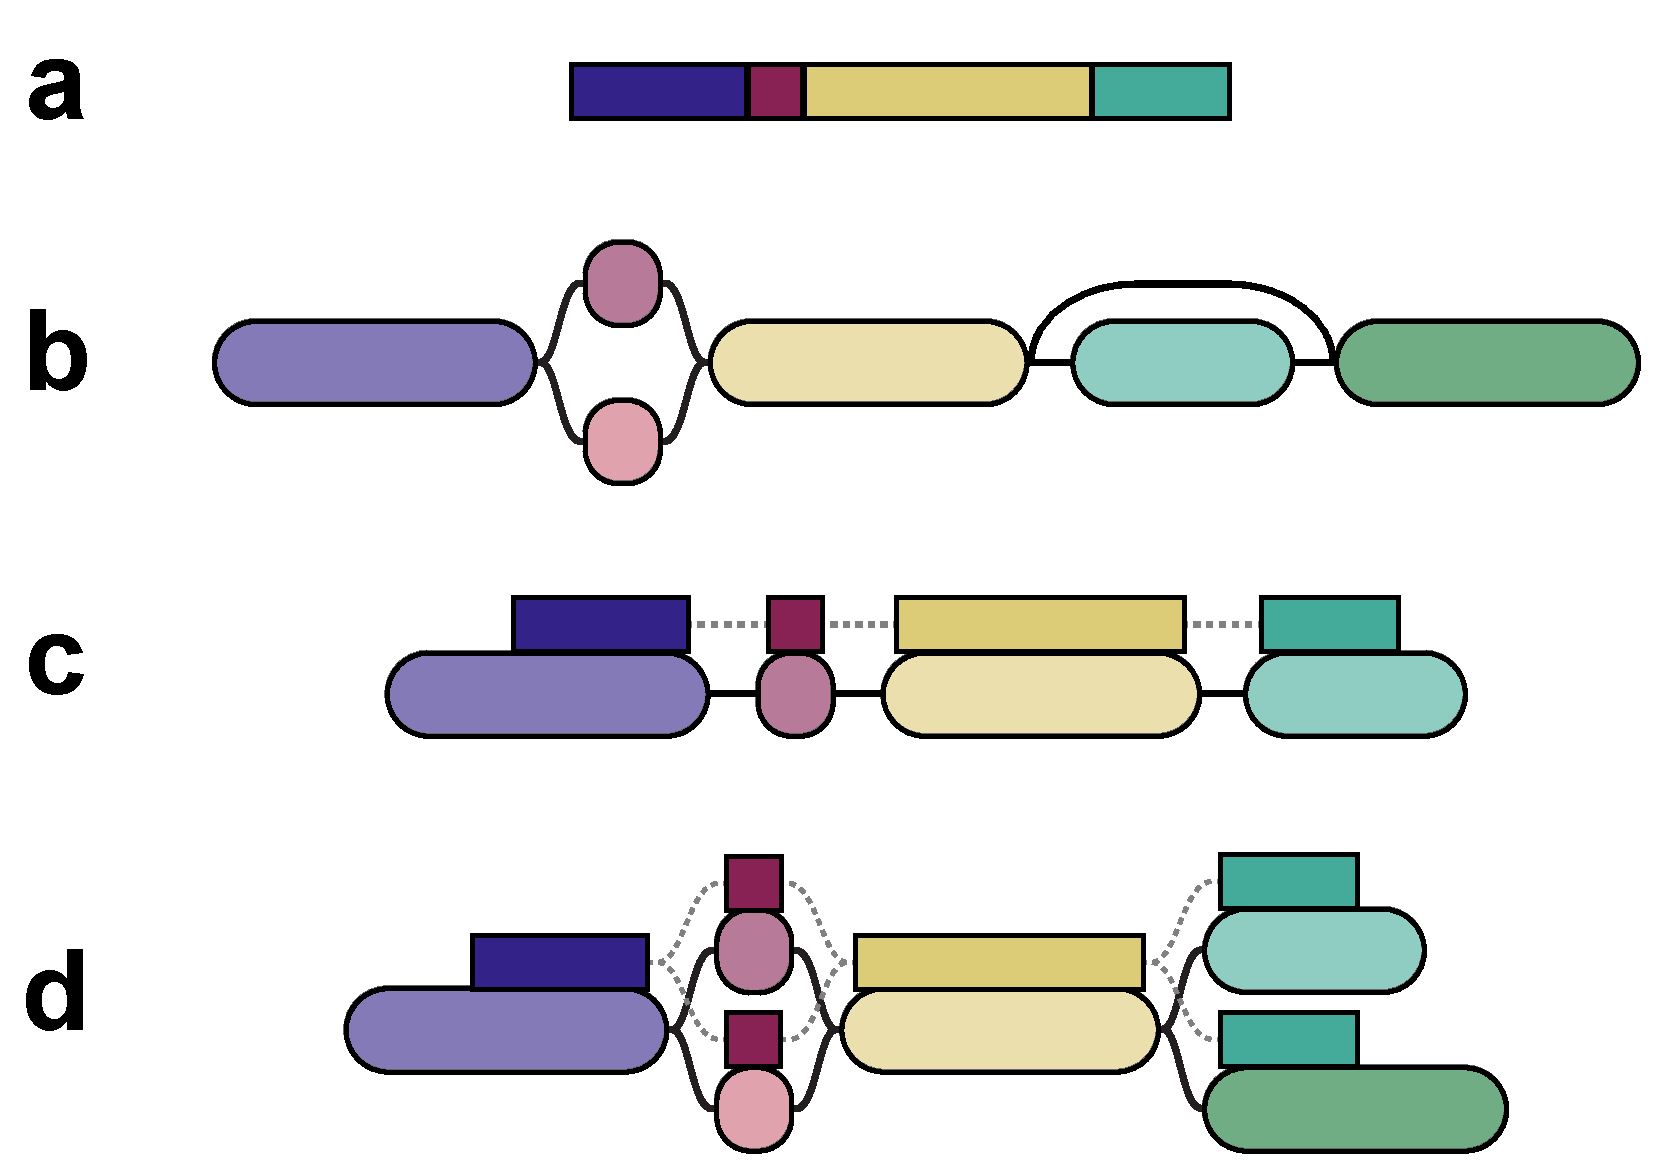
\includegraphics[width=0.8\textwidth]{mpmapfigures/figureS10.pdf}
\caption{\textbf{Diagram of a multipath alignment} \\
A diagrammatic comparison between the multipath alignment output of vg mpmap and the single-path alignment output of other graph aligners (such as vg map). \textbf{a} A read and \textbf{b} a sequence graph, which have been colored to indicate which parts of the read could plausibly align to which parts of the graph. \textbf{c} A single-path alignment. The read sequence is aligned to one path from the graph. \textbf{d} A multipath alignment. The alignment can split and rejoin to express the alignment uncertainty to different paths in the graph.
} \label{fig:multipath-alignment}
\end{center}
\end{figure}

\begin{figure}[H]
\ssp
\begin{center}
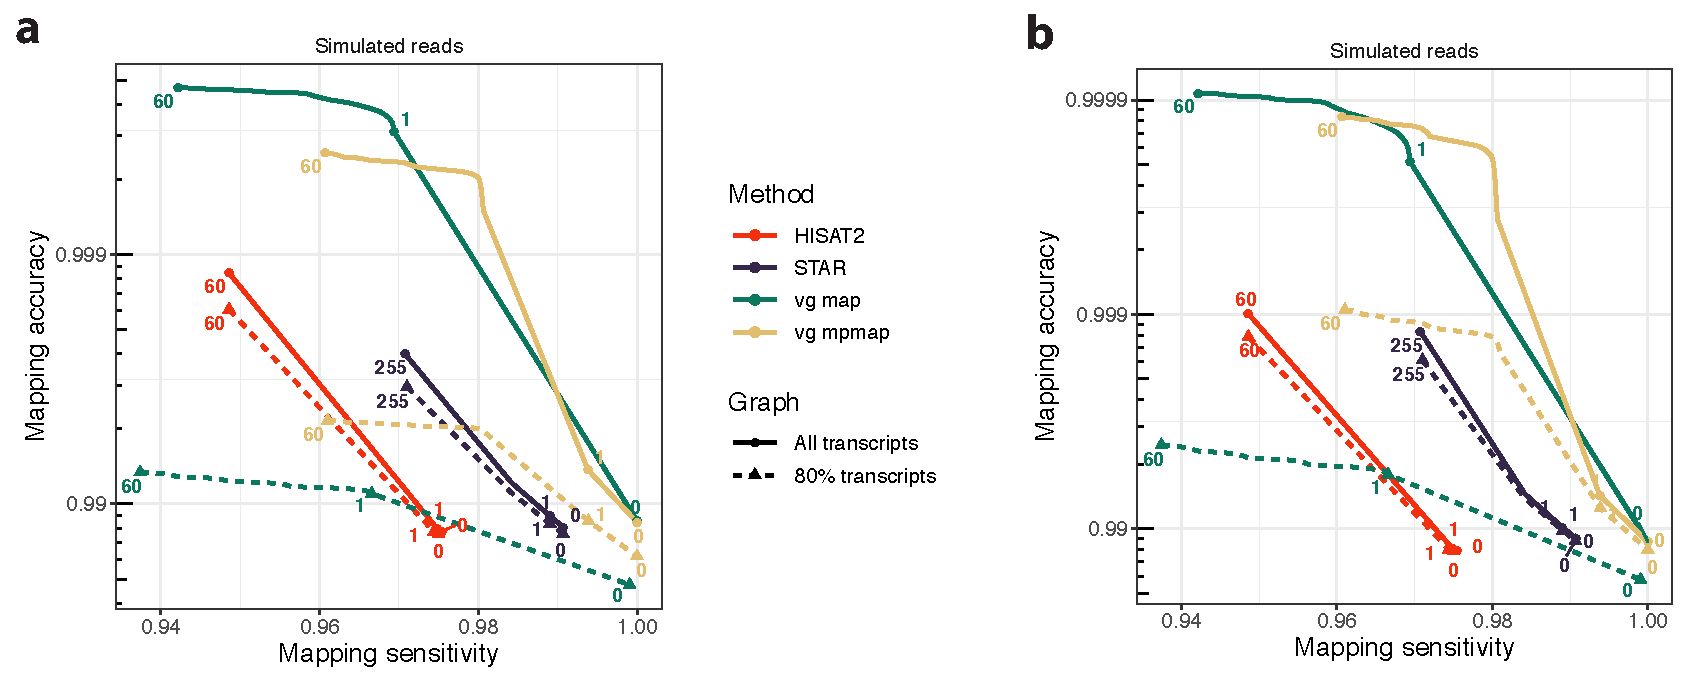
\includegraphics[width=\textwidth]{mpmapfigures/figureS1.pdf}
\caption{\textbf{Mapping benchmark to novel splice-junctions using RNA-seq data from NA12878} \\
RNA-seq mapping results comparing vg mpmap against three other methods using simulated Illumina data (``vg sim (ENC, uniform)'' in Supplementary Table \ref{tab:sim-data}). Shows mapping accuracy and sensitivity for different mapping quality thresholds (colored numbers). An alignment is considered correct if it covers 90\% (\textbf{a}) or 70\% (\textbf{b}) of the true reference sequence alignment. Solid lines show the results using a spliced pangenome graph (spliced reference for STAR) generated using the complete transcript annotation. Dashed lines show the results using a reference generated with a random subset of 80\% of the transcripts in the annotation.
} \label{fig:splice-junction-mapping}
\end{center}
\end{figure}

\begin{figure}[H]
\ssp
\begin{center}
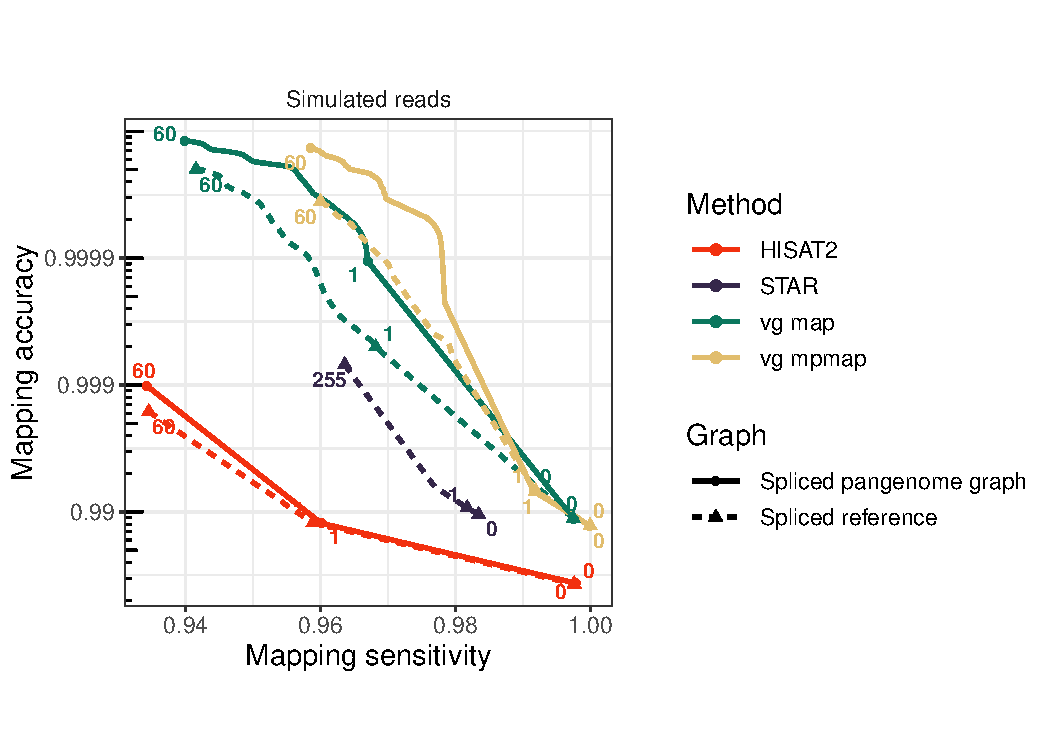
\includegraphics[width=0.8\textwidth]{mpmapfigures/figureS2.pdf}
\caption{\textbf{Graph-based mapping benchmark using RNA-seq data from NA12878} \\
Mapping accuracy and sensitivity for vg mpmap and three other methods using simulated Illumina data (``vg sim (ENC, uniform)'' in Supplementary Table \ref{tab:sim-data}). Colored numbers indicate different mapping quality thresholds. An alignment is considered correct if its start position is within 100 bases from the start position of the true alignment measured using any labeled transcript path in the graph or the linear reference sequence. Solid and dashed lines show the results using a spliced pangenome graph and spliced reference, respectively. 
} \label{fig:mapping-gampcompare}
\end{center}
\end{figure}


\begin{figure}[H]
\ssp
\begin{center}
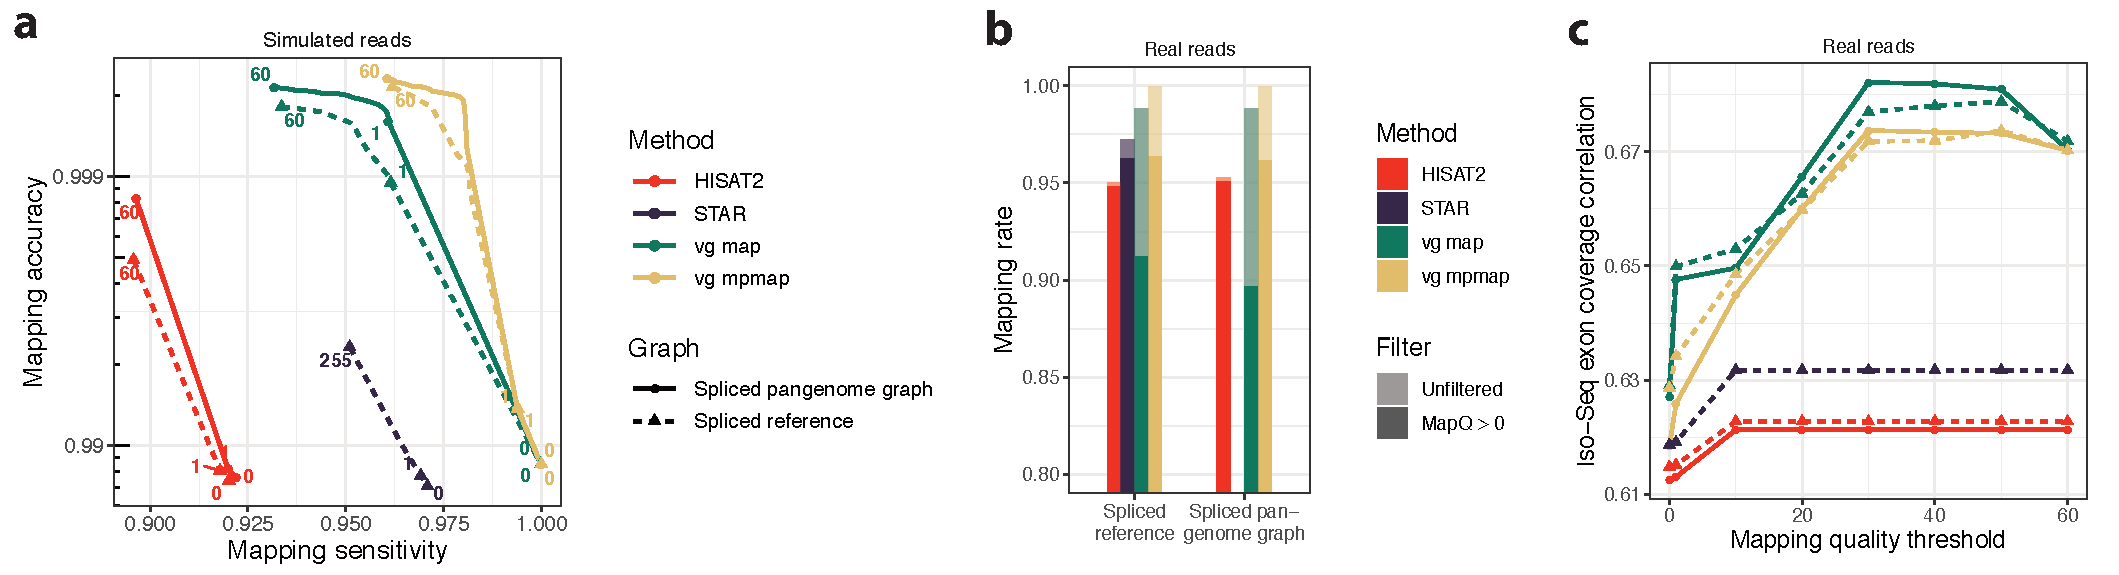
\includegraphics[width=\textwidth]{mpmapfigures/figureS3.pdf}
\caption{\textbf{Mapping benchmark using RNA-seq training data from NA12878} \\
RNA-seq mapping results comparing vg mpmap and three other methods using the simulated and real Illumina data that was used in the optimization of vg map and vg mpmap (``vg sim (SRR, uniform)'' and ``SRR1153470'' in Supplementary Table \ref{tab:sim-data} and \ref{tab:read-sets}, respectively). Solid and dashed lines show the results using a spliced pangenome graph and spliced reference, respectively. \textbf{a} Mapping accuracy and sensitivity for different mapping quality thresholds (colored numbers) using simulated data. An alignment is considered correct if it covers 90\% of the true reference sequence alignment. \textbf{b} Mapping rate using real data. The shaded bars show the mapping rate for all alignments and the solid bars for only alignments with a mapping quality above 0. \textbf{c} Pearson correlation between Illumina and Iso-Seq exon coverage using real data as a function of mapping quality threshold. Exons are defined by the Iso-Seq alignments.
} \label{fig:mapping-srr}
\end{center}
\end{figure}

\begin{figure}[H]
\ssp
\begin{center}
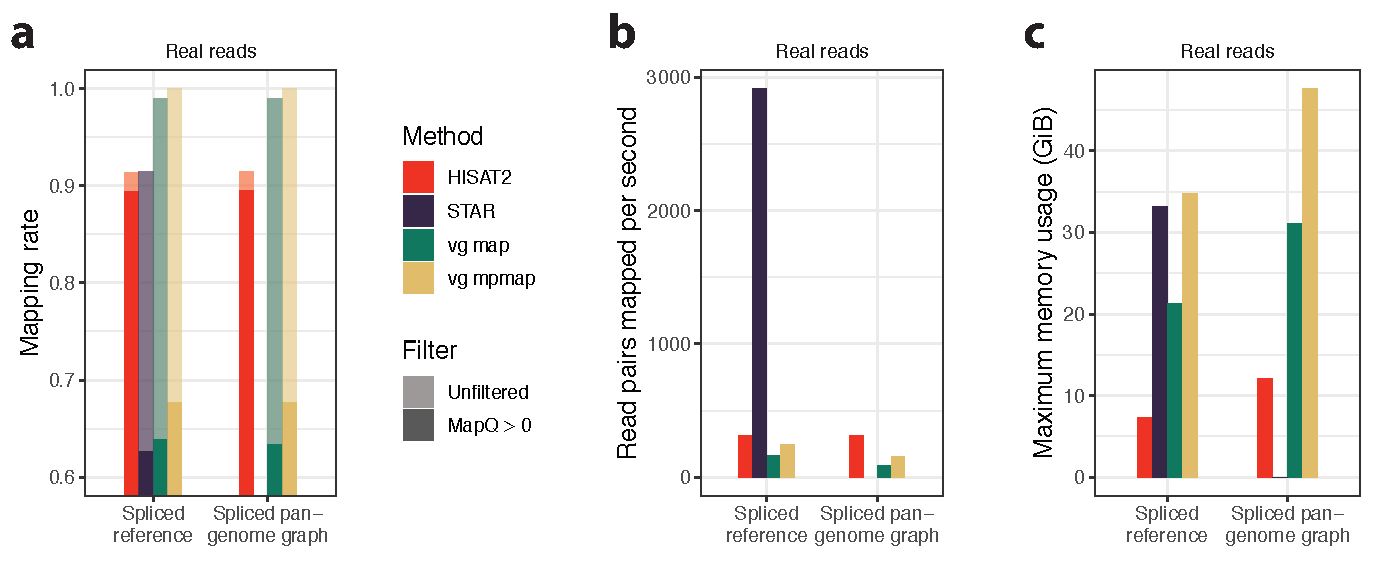
\includegraphics[width=\textwidth]{mpmapfigures/figureS4.pdf}
\caption{\textbf{Mapping benchmark using RNA-seq training data from CHM13} \\
RNA-seq mapping results comparing vg mpmap against three other methods using real Illumina data that was used in the optimization of vg mpmap (``CHM13'' in Supplementary Table \ref{tab:read-sets}). \textbf{a} Mapping rate. The shaded bars show the mapping rate for all alignments and the solid bars for only alignments with a mapping quality above 0. \textbf{b} Number of read pairs mapped per second per thread. The mapping times were measured using 16 threads on a AWS m5.4xlarge instance. \textbf{c} Maximum memory usage for mapping in gigabytes. 
} \label{fig:mapping-t2t}
\end{center}
\end{figure}

\begin{figure}[H]
\ssp
\begin{center}
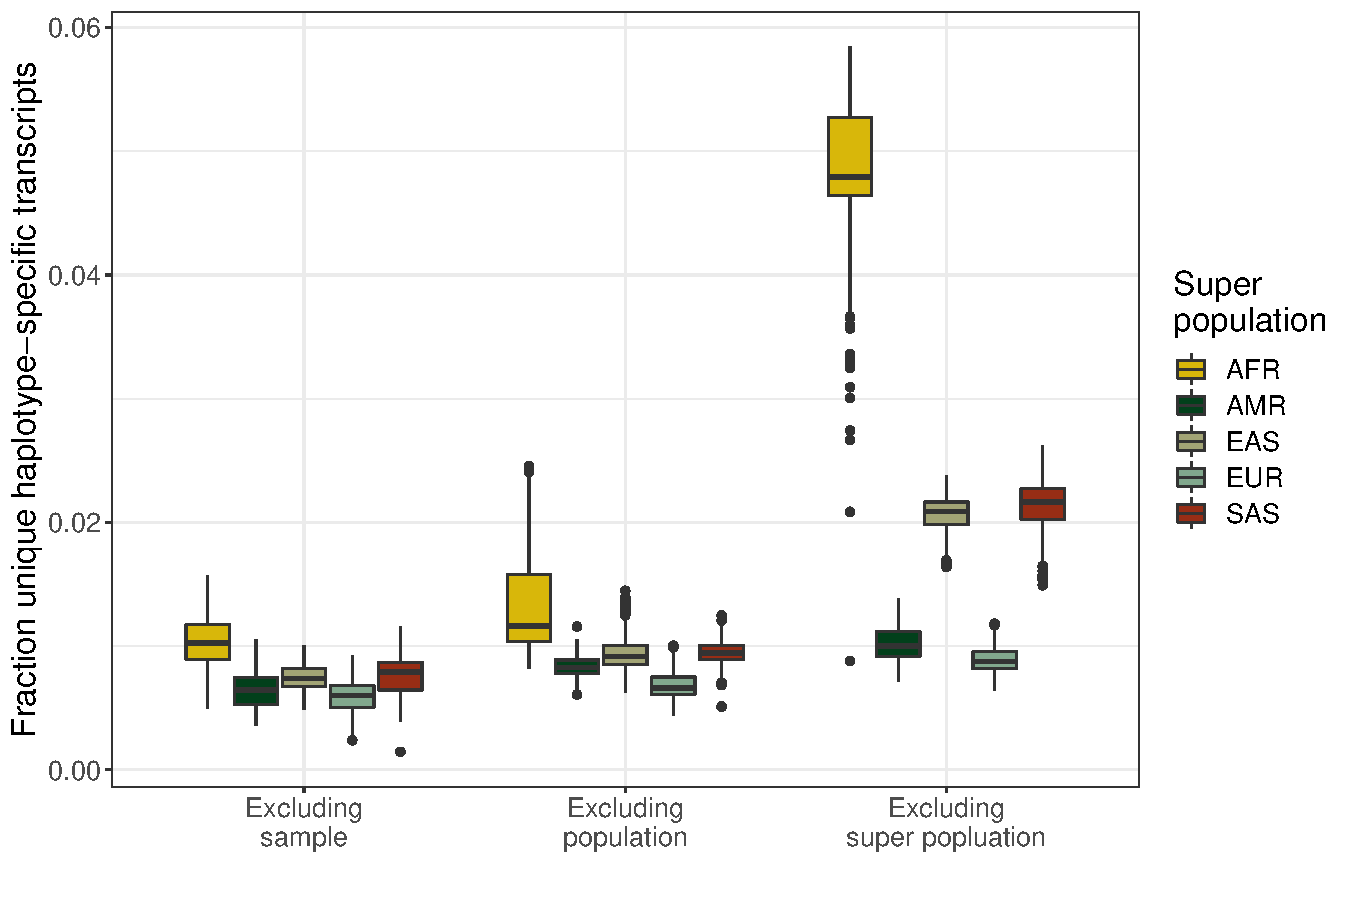
\includegraphics[width=0.8\textwidth]{mpmapfigures/figureS5.pdf}
\caption{\textbf{Haplotype-specific transcript uniqueness in a 1000 Genomes Project pantranscriptome} \\
The fraction of HSTs that are unique to each sample in the 1000 Genomes Project (1000GP) when compared to different subsets of samples in the 1000GP. Left box plots show the fraction unique when comparing to all other samples, middle box plots show the fraction unique when comparing to all other samples excluding the samples’ population, and right box plots show the fraction unique when comparing to all other samples excluding the samples’ super population. AFR: African, AMR: Admixed American, EAS: East Asian, EUR: European, SAS: South Asian.
} \label{fig:hst-populations}
\end{center}
\end{figure}

\begin{figure}[H]
\ssp
\begin{center}
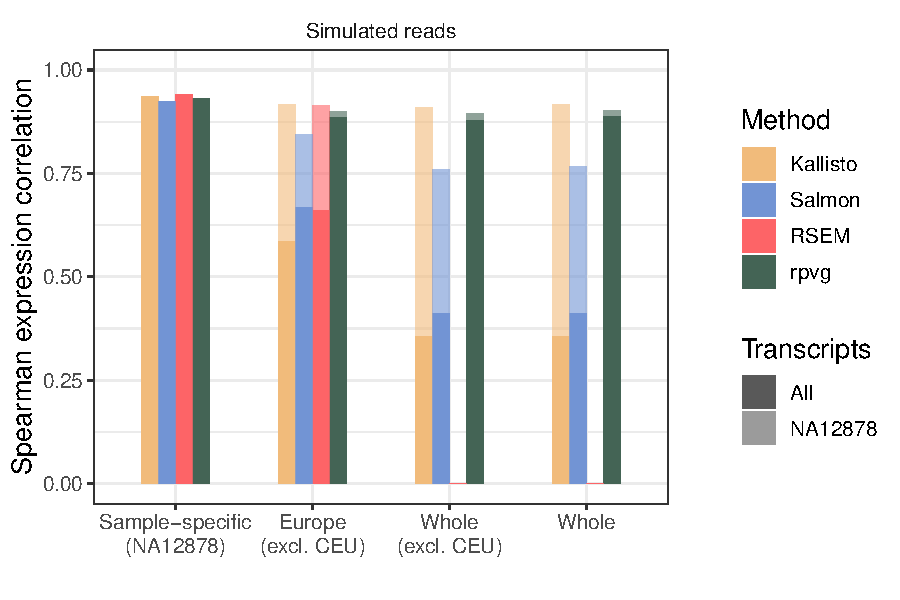
\includegraphics[width=0.8\textwidth]{mpmapfigures/figureS6.pdf}
\caption{\textbf{Haplotype-specific transcript expression correlation benchmark using RNA-seq data from NA12878} \\
Haplotype-specific transcript (HST) quantification results comparing rpvg and three other methods using simulated Illumina data (``vg sim (ENC, RSEM)'' in Supplementary Table \ref{tab:sim-data}). Shows Spearman correlation between simulated and estimated expression (in transcripts per million (TPM)) for different pantranscriptomes. Correlation was calculated using either all HSTs in the pantranscriptome (solid bars) or using only the NA12878 HSTs (shaded bars). ``Sample-specific (NA12878)'' is a personal transcriptome generated from 1000 Genomes Project (1000GP) NA12878 haplotypes. ``Europe (excl. CEU)'' is a pantranscriptome generated from European 1000GP haplotypes excluding the CEU population. ``Whole (excl. CEU)'' and ``Whole'' are pantranscriptomes generated from all 1000GP haplotypes without and with the CEU population, respectively. 
} \label{fig:expression-corr}
\end{center}
\end{figure}

\begin{figure}[H]
\ssp
\begin{center}
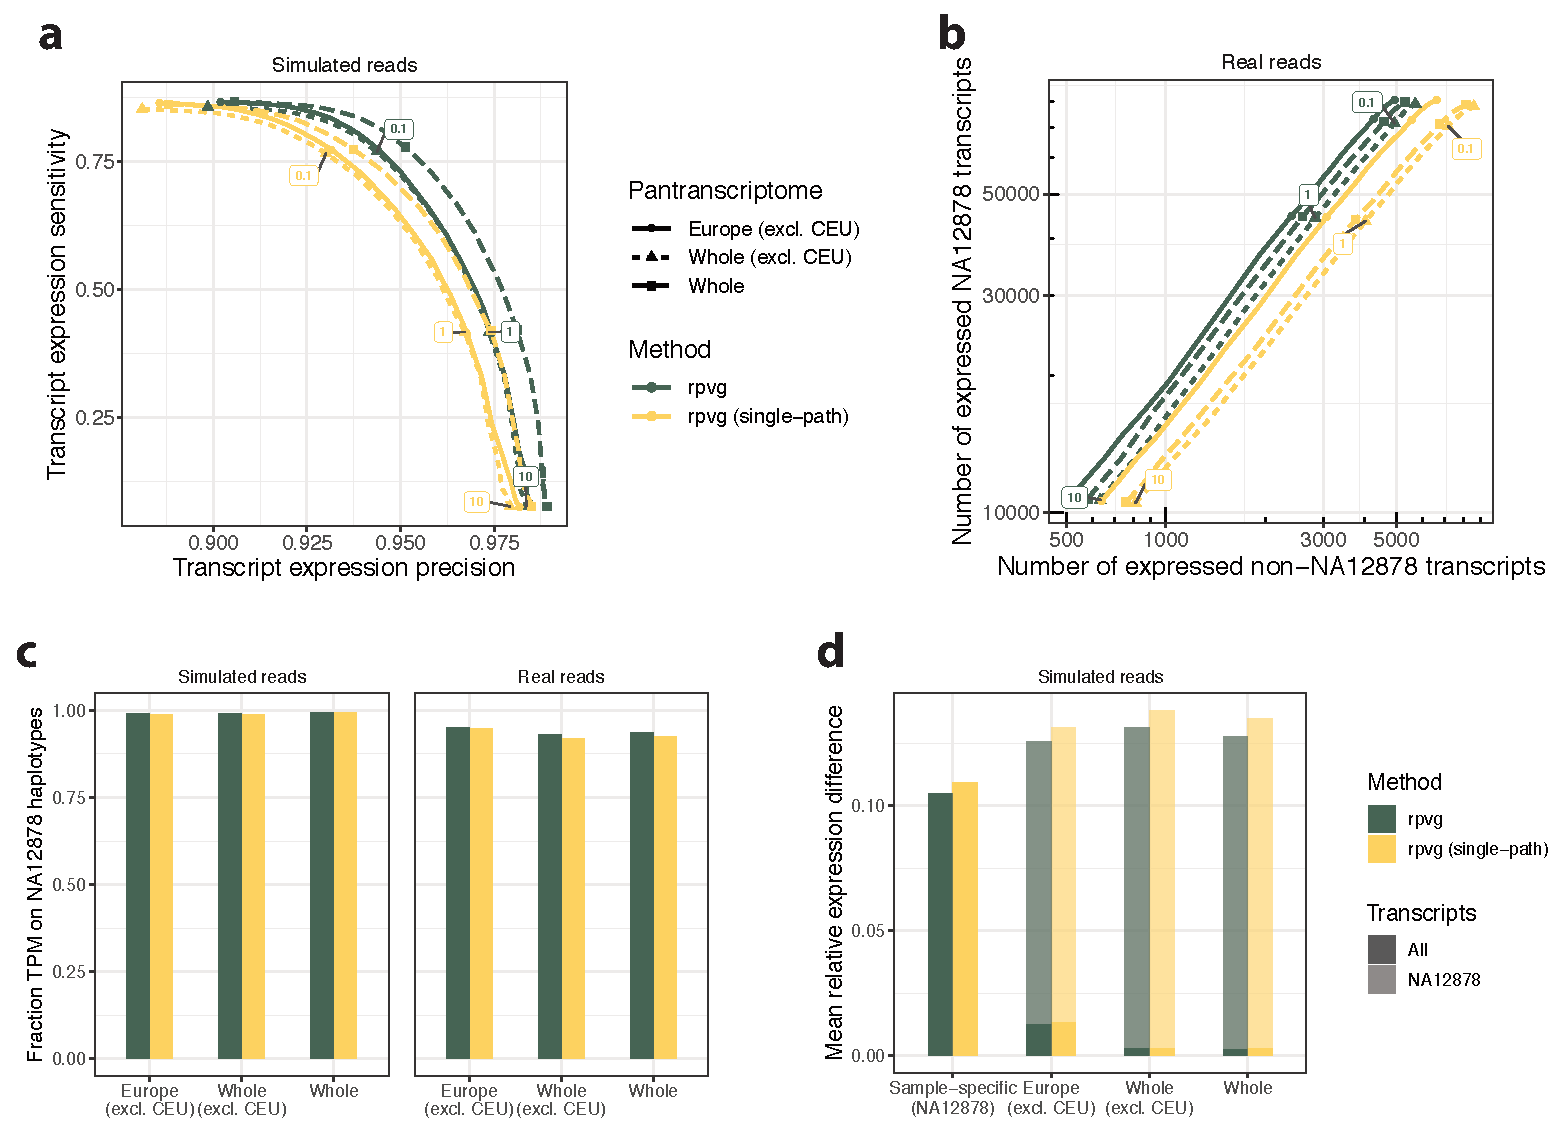
\includegraphics[width=\textwidth]{mpmapfigures/figureS7.pdf}
\caption{\textbf{Multipath alignment benchmark using RNA-seq data from NA12878} \\
Haplotype-specific transcript (HST) quantification results comparing rpvg with single-path and multipath alignments using simulated and real Illumina data (``vg sim (ENC, RSEM)'' and ``ENCSR000AED'' in Supplementary Table \ref{tab:sim-data} and \ref{tab:read-sets}, respectively). Solid lines with circles are results using a pantranscriptome generated from 1000 Genomes Project (1000GP) European haplotypes excluding the CEU population. Dashed lines with triangles and squares are results using a pantranscriptome generated from all 1000GP haplotypes without and with the CEU population, respectively. The single-path alignments were created by finding the best scoring path in each multipath alignment. \textbf{a} Sensitivity and precision of whether a transcript is correctly assigned nonzero expression for different expression value thresholds (colored numbers for ``Whole (excl. CEU)'' pantranscriptome) using simulated data. Expression is measured in transcripts per million (TPM). \textbf{b} Number of expressed transcripts from NA12878 haplotypes shown against the number from non-NA12878 haplotypes for different expression value thresholds (colored numbers) using real data. \textbf{c} Fraction of transcript expression (in TPM) assigned to NA12878 haplotypes for different pantranscriptomes using simulated (left) and real (right) data. \textbf{d} Mean absolute relative difference (MARD) between simulated and estimated expression (in TPM) for different pantranscriptomes using simulated data. MARD was calculated using either all HSTs in the pantranscriptome (solid bars) or using only the NA12878 HSTs (shaded bars). ``Sample-specific (NA12878)'' is a personal transcriptome generated from 1000GP NA12878 haplotypes.
} \label{fig:expression-multipath}
\end{center}
\end{figure}

\begin{figure}[H]
\ssp
\begin{center}
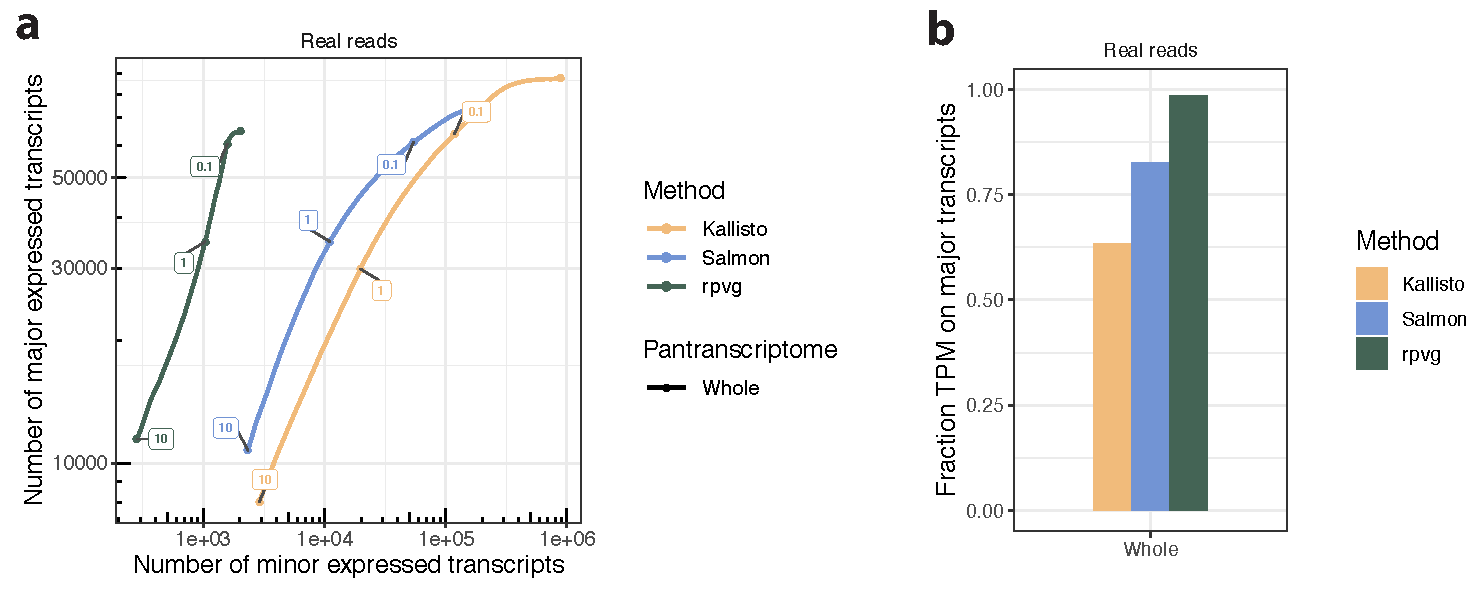
\includegraphics[width=\textwidth]{mpmapfigures/figureS8.pdf}
\caption{\textbf{Haplotype-specific transcript quantification benchmark using RNA-seq training data from CHM13} \\
Haplotype-specific transcript (HST) quantification results comparing rpvg against two other methods using real Illumina data that was used in the optimization of rpvg (``CHM13'' in Supplementary Table \ref{tab:read-sets}). All experiments used a pantranscriptome generated from all 1000 Genomes Project (1000GP) haplotypes. Each HST is either classified as major or minor. Major HSTs are defined as the highest expressed haplotype for each transcript; the rest are defined as minor. As CHM13 is effectively haploid, the fraction of expression from minor HSTs is a lower bound on the fraction of incorrectly inferred transcript expression. \textbf{a} Number of major expressed transcripts against the number of minor expressed for different expression value thresholds (colored numbers). Expression is measured in transcripts per million (TPM). \textbf{b} Fraction of transcript expression (in TPM) assigned to major transcripts for different methods.
} \label{fig:expression-t2t}
\end{center}
\end{figure}

\begin{figure}[H]
\ssp
\begin{center}
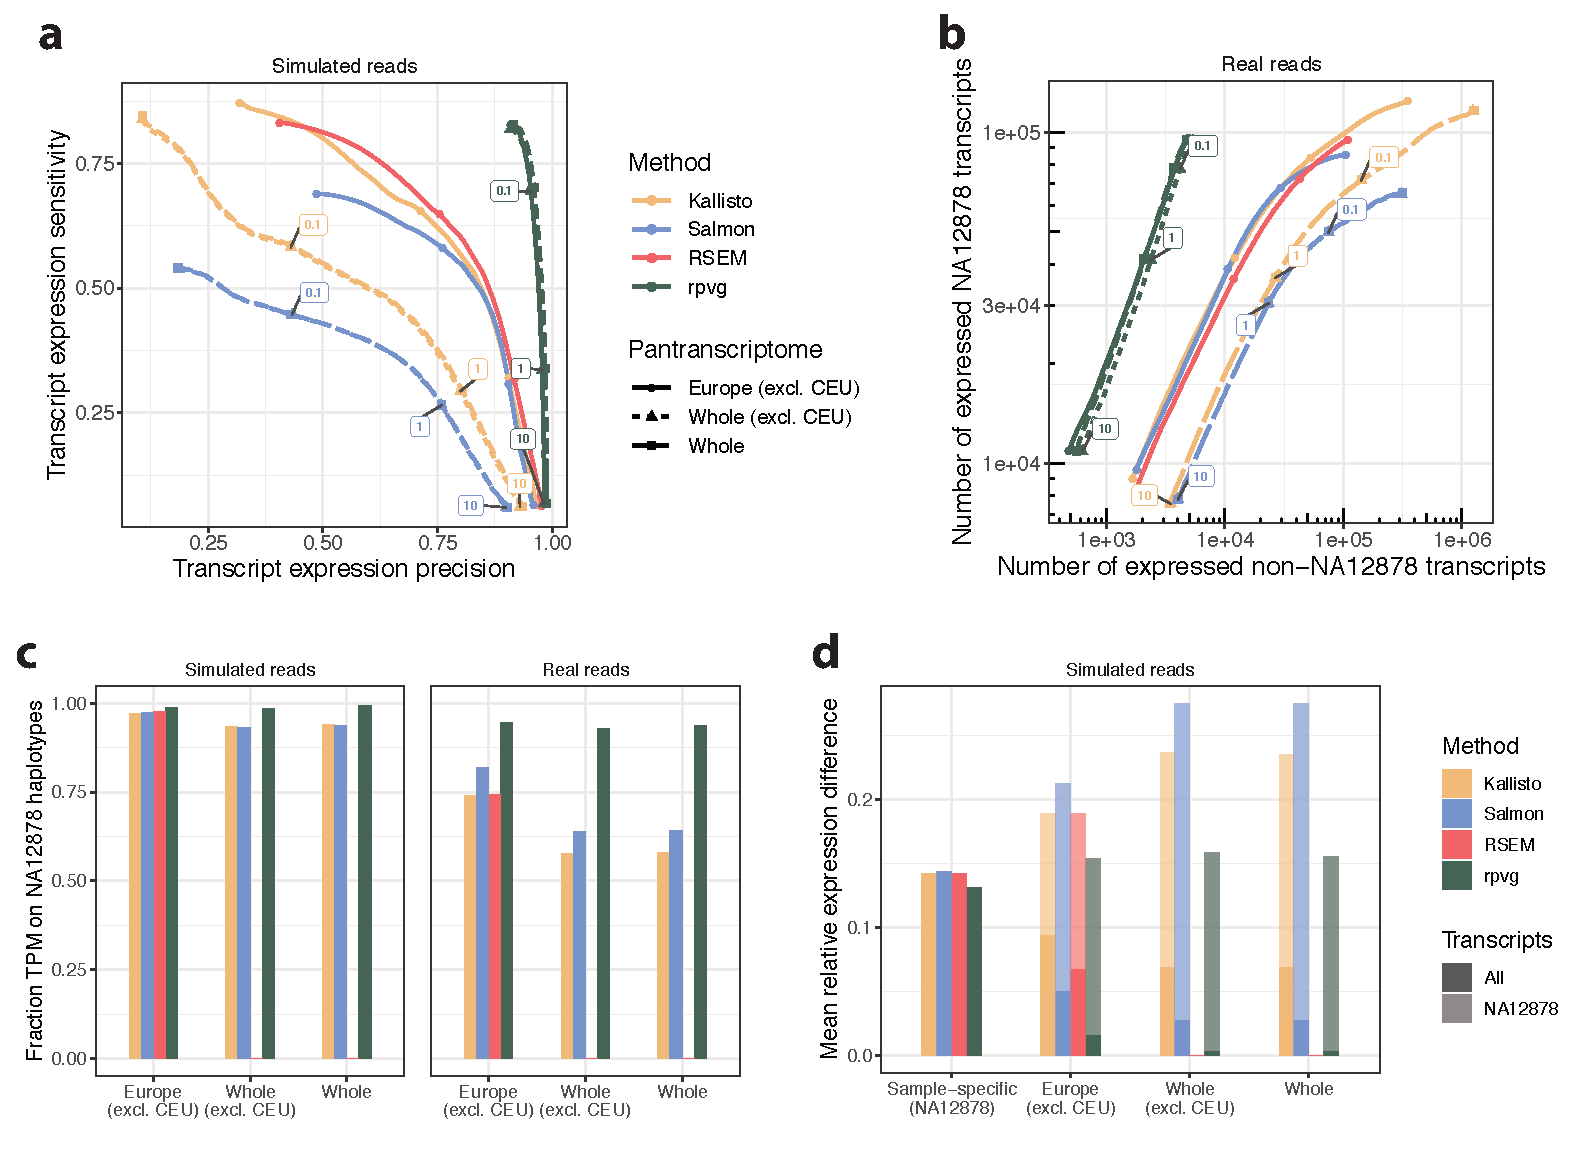
\includegraphics[width=\textwidth]{mpmapfigures/figureS9.pdf}
\caption{\textbf{Haplotype-specific transcript quantification benchmark using RNA-seq training data from NA12878} \\
Haplotype-specific transcript (HST) quantification results comparing rpvg against three other methods using simulated and real Illumina data that was used in the optimization of rpvg (``vg sim (SRR, RSEM)'' and ``SRR1153470'' in Supplementary Table \ref{tab:sim-data} and \ref{tab:read-sets}, respectively). Solid lines with circles are results using a pantranscriptome generated from 1000 Genomes Project (1000GP) European haplotypes excluding the CEU population. Dashed lines with triangles and squares are results using a pantranscriptome generated from all 1000GP haplotypes without and with the CEU population, respectively. \textbf{a} Sensitivity and precision of whether a transcript is correctly assigned nonzero expression for different expression value thresholds (colored numbers for ``Whole (excl. CEU)'' pantranscriptome) using simulated data. Expression is measured in transcripts per million (TPM). \textbf{b} Number of expressed transcripts from NA12878 haplotypes shown against the number from non-NA12878 haplotypes for different expression value thresholds (colored numbers) using real data. \textbf{c} Fraction of transcript expression (in TPM) assigned to NA12878 haplotypes for different pantranscriptomes using simulated (left) and real (right) data. \textbf{d} Mean absolute relative difference (MARD) between simulated and estimated expression (in TPM) for different pantranscriptomes using simulated data. MARD was calculated using either all HSTs in the pantranscriptome (solid bars) or using only the NA12878 HSTs (shaded bars). ``Sample-specific (NA12878)'' is a personal transcriptome generated from 1000GP NA12878 haplotypes.
} \label{fig:expression-srr}
\end{center}
\end{figure}
 
\begin{figure}[H]
\ssp
\begin{center}
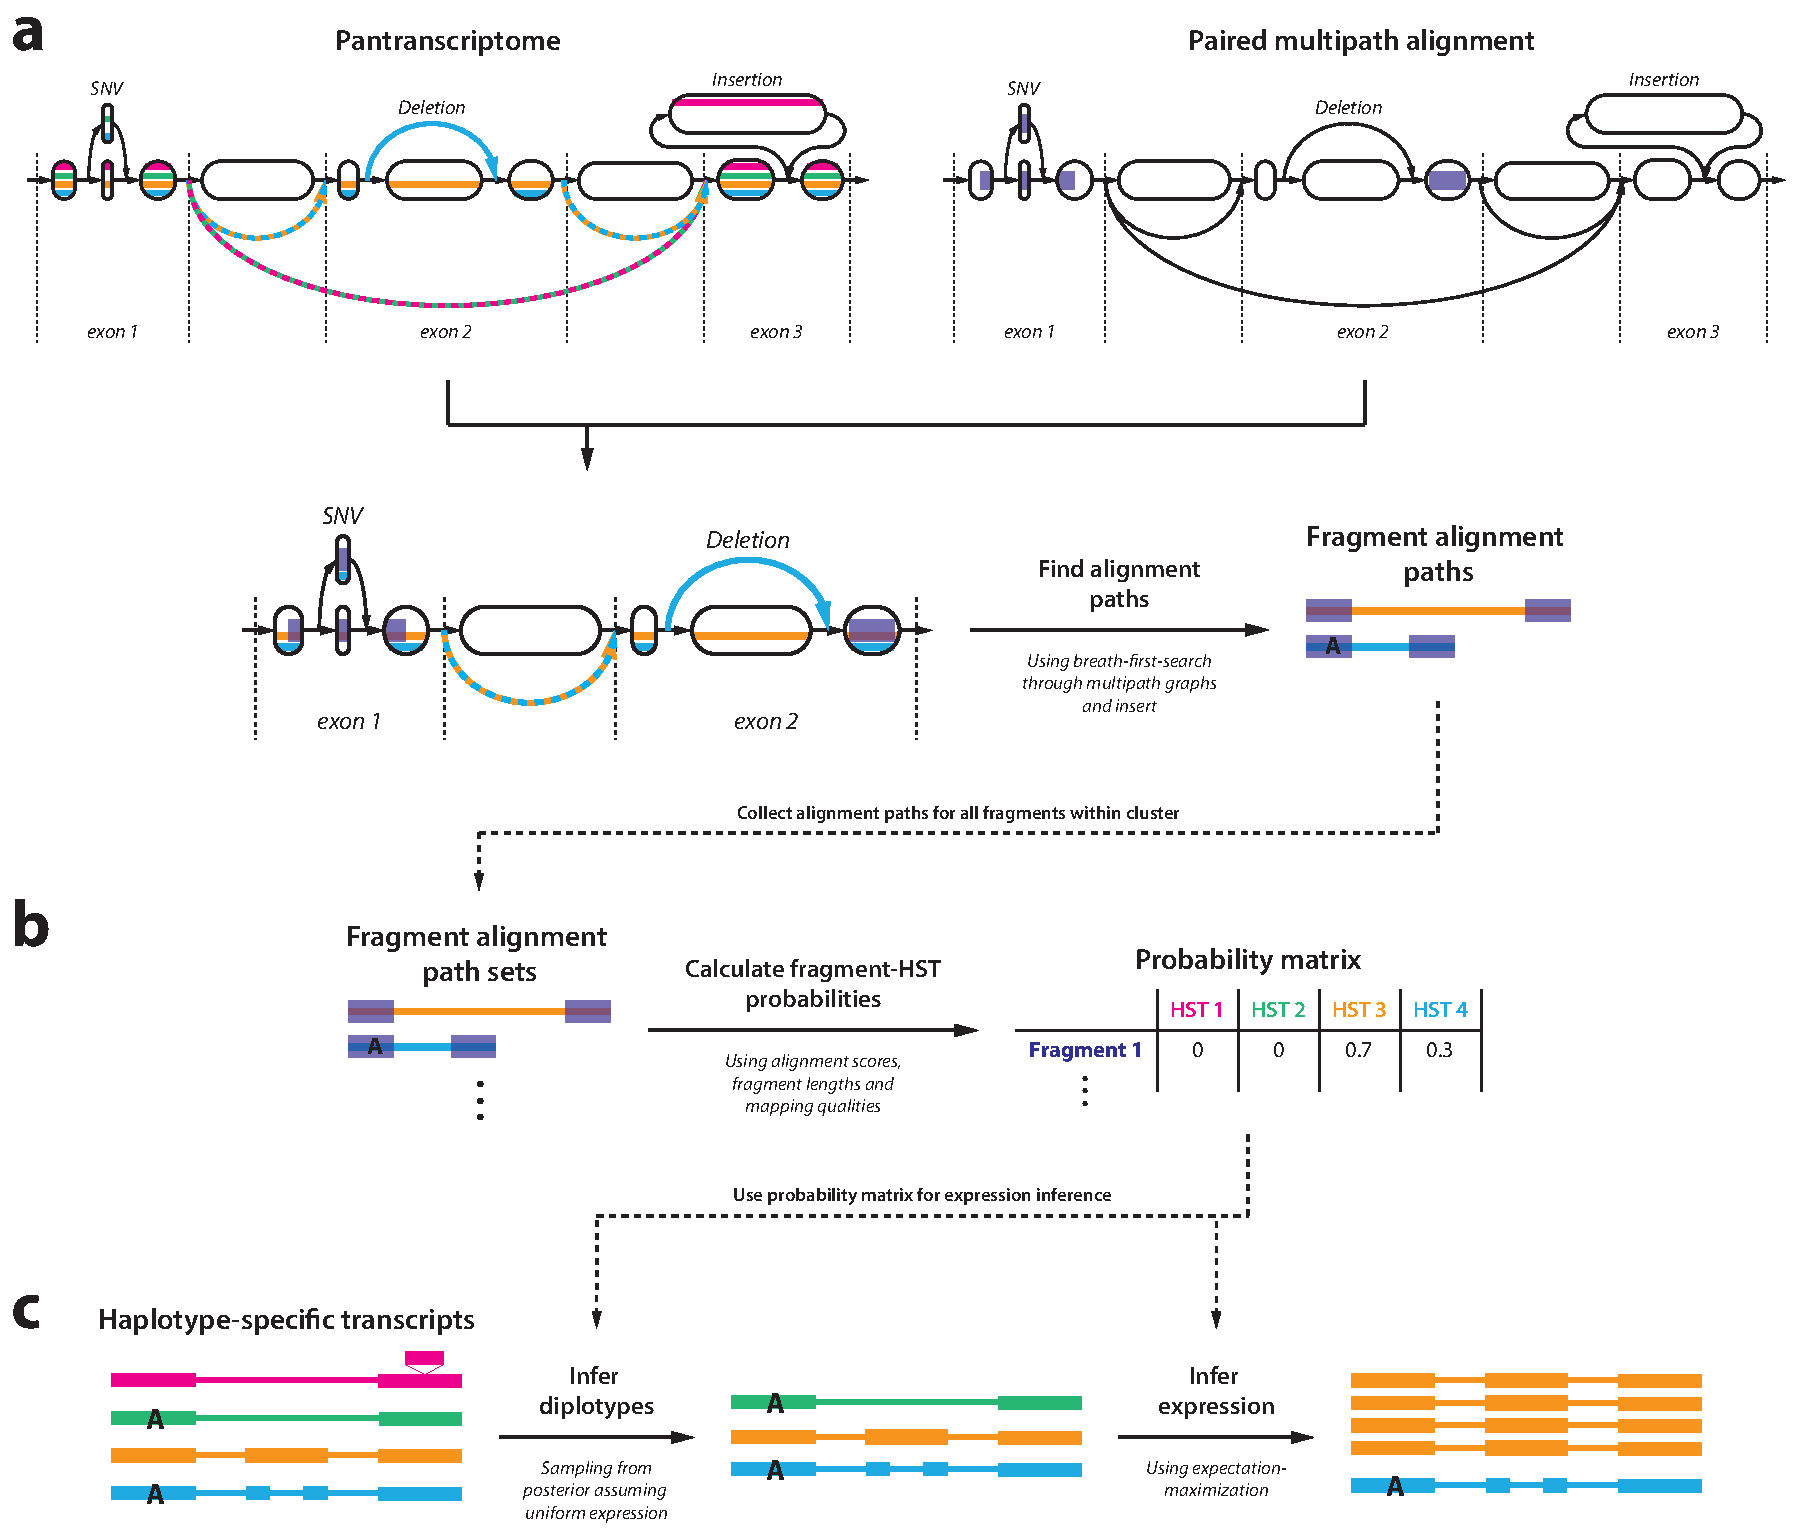
\includegraphics[width=\textwidth]{mpmapfigures/figureS11.pdf}
\caption{\textbf{Diagram of haplotype-specific transcript quantification in rpvg
} \\
Diagram showing an overview of how rpvg infers expression of haplotype-specific transcripts (HSTs) in a pantranscriptome from a set of paired-end multipath alignments (see Supplementary Figure 10). The colored thin lines correspond to HST paths, and the blue transparent regions correspond to aligned read sequences. \textbf{a} For each fragment, all paths through the multipath alignment graphs are identified using a depth-first-search (DFS). For paired-end reads, the DFS also traverses the fragment insert creating alignment paths of the whole fragment. Only alignment paths that follow an HST path in the pantranscriptome are kept. \textbf{b} The probabilities that each fragment originated from each of the HSTs in a cluster are calculated using the score and length of the fragment alignment paths, and the mapping quality. \textbf{c} The fragment-HST probability matrix is used to infer the expression of the HSTs using a nested inference scheme. First, a distribution over diplotypes (if sample is diploid) is inferred. A haplotype combination is then sampled from this distribution and expression is inferred conditioned on the sampled haplotypes using expectation-maximization. This procedure is repeated a 1,000 times to account for the uncertainty in the haplotype estimates.
} \label{fig:hst-quantification}
\end{center}
\end{figure}

\section{Supplementary Tables}

\begin{table}[H]
\ssp
\footnotesize
\begin{tabular}{L{0.13\textwidth}| L{0.25\textwidth} | R{0.12\textwidth} | R{0.1\textwidth} | R{0.11\textwidth} | R{0.11\textwidth}}
\textbf{Name} & \textbf{Description} & \textbf{Non-exonic variant filter} & \textbf{Number of samples} & \textbf{Number of exonic variants} & \textbf{Number of total variants} \\
\midrule
1000GP (NA12878)& 1000GP variants observed in NA12878 & None & 1 & 152,968 & 4,266,678 \\
\midrule
1000GP (EUR, excl. CEU) & All european (EUR) 1000GP variants excluding variants unique to the CEU population & AF $\geq$ 0.002 & 404 & 986,167 & 15,041,731 \\
\midrule
1000GP (all, excl. CEU) & All 1000GP variants excluding variants unique to the CEU population & AF $\geq$ 0.001 & 2,405 & 3,808,242 & 31,731,676 \\
\midrule
1000GP (all) & All 1000GP variants & AF $\geq$ 0.001 & 2,504 & 3,873,100 & 29,970,512
\end{tabular}
\caption{\textbf{Genomic variant (haplotype) sets} \\
1000GP: 1000 Genomes Project}
\label{tab:haplotype-sets}
\end{table}

\begin{table}[H]
\ssp
\footnotesize
\begin{tabular}{L{0.13\textwidth} | L{0.14\textwidth} | R{0.12\textwidth} | L{0.13\textwidth} | R{0.11\textwidth} | R{0.17\textwidth}}
\textbf{Name} & \textbf{Transcript annotation} & \textbf{Number of transcripts} & \textbf{Haplotype set}$\dag$ & \textbf{Number of haplotypes} & \textbf{Number of haplotype-specific transcripts} \\
\midrule
Sample-specific (NA12878)& GENCODE v29 (full-length) & 172,449 & 1000GP (NA12878) & 2 & 235,400 \\
\midrule
Europe (excl. CEU) & GENCODE v29 (full-length) & 172,449 & 1000GP (EUR, excl. CEU) & 808 & 2,515,408 \\
\midrule
Whole (excl. CEU) & GENCODE v29 (full-length) & 172,449 & 1000GP (all, excl. CEU) & 4,810 & 11,626,948 \\
\midrule
Whole & GENCODE v29 (full-length) & 172,449 & 1000GP (all) & 5,008 & 11,835,580
\end{tabular}
\caption{\textbf{Pantranscriptomes}\\
$\dag$See Supplementary Table \ref{tab:haplotype-sets} for more details on the haplotype sets
}
\label{tab:pantranscriptomes}
\end{table}

\begin{table}[H]
\ssp
\footnotesize
\begin{tabular}{L{0.15\textwidth}| L{0.1\textwidth} | L{0.09\textwidth} | L{0.09\textwidth} | L{0.17\textwidth} | R{0.16\textwidth}}
\textbf{Name / Accession (source)} & \textbf{Reference} & \textbf{Replicate} & \textbf{Cell-line} & \textbf{Sequencing type} & \textbf{Number of read-pairs or alignments} \\
\midrule
SRR1153470 (SRA) & \cite{tilgner2014defining} & NA & NA12878 & Paired-end Illumina HiSeq 2000 & 115,359,773 read-pairs \\
\midrule
ENCSR000AED (ENCODE) & \cite{encode2012integrated,davis2017encycolopedia} & 1 & NA12878 & Paired-end Illumina HiSeq 2000 & 97,548,052 read-pairs \\
\midrule
ENCSR706ANY (ENCODE) & \cite{encode2012integrated,davis2017encycolopedia} & 1-4 & NA12878 & PacBio Iso-Seq & 2,687,717 alignments \\
\midrule
CHM13 (T2T) & $\dag$ & 1 & CHM13 & Paired-end Illumina NovaSeq & 90,930,105  read-pairs \\ 
\midrule
ERR188217 \& ERR204848 (Geuvadis) & \cite{lappalainen2013transcriptome} & 1 & NA11832 & Paired-end Illumina HiSeq 2000 & 2,354,918 + 863,919 read-pairs \\
\midrule
ERR188235 \& ERR204834 (Geuvadis) & \cite{lappalainen2013transcriptome} & 1 & NA11930 & Paired-end Illumina HiSeq 2000 & 1,305,660 + 1,220,864 read-pairs \\
\midrule
ERR188354 \& ERR204977 (Geuvadis) & \cite{lappalainen2013transcriptome} & 1 & NA12775 & Paired-end Illumina HiSeq 2000 & 3,088,867 + 806,975 read-pairs \\
\midrule
ERR188429 \& ERR204822 (Geuvadis) & \cite{lappalainen2013transcriptome} & 1 & NA12889 & Paired-end Illumina HiSeq 2000 & 2,286,090 + 778,671 read-pairs
\end{tabular}
%}
\caption{\textbf{Read sets and alignments}\\
$\dag$Downloaded from the T2T consortium data repository:\\ \protect\url{https://github.com/nanopore-wgs-consortium/CHM13}
}
\label{tab:read-sets}
\end{table}

\begin{table}[H]
\ssp
\footnotesize
\begin{tabular}{L{0.12\textwidth}| L{0.14\textwidth} | L{0.13\textwidth} | L{0.12\textwidth} | L{0.15\textwidth} | R{0.11\textwidth}}
\textbf{Name} & \textbf{Training reads}$\dag$ & \textbf{Haplotype-specific transcripts}$\ddag$ & \textbf{Expression values} & \textbf{vg sim parameters} & \textbf{Number of read-pairs} \\
\midrule
vg sim (SRR, uniform) & SRR1153470 & Sample-specific (NA12878) & Uniform& Indel error: 0.001, mean: 277, sd: 43 & 50,000,000 \\
\midrule
vg sim (ENC, uniform) & ENCSR000AED & Sample-specific (NA12878) & Uniform & Indel error: 0.001, mean: 216, sd: 24 & 50,000,000 \\
\midrule
vg sim (SRR, RSEM) & SRR1153470 & Sample-specific (NA12878) & RSEM estimates & Indel error: 0.001, mean: 277, sd: 43 & 50,000,000 \\
\midrule
vg sim (ENC, RSEM) & ENCSR000AED & Sample-specific (NA12878) & RSEM estimates & Indel error: 0.001, mean: 216, sd: 24 & 50,000,000
\end{tabular}
%}
\caption{\textbf{Simulated read sets}\\
$\dag$See Supplementary Table \ref{tab:read-sets} for more details on the training read sets \\
$\ddag$See Supplementary Table \ref{tab:pantranscriptomes} for more details on the haplotype-specific transcript sets}
\label{tab:sim-data}
\end{table}

\begin{table}[H]
\ssp
\footnotesize
\begin{tabular}{L{0.2\textwidth}| L{0.4\textwidth} | R{0.18\textwidth}}
\textbf{Software tool(s) or library} & \textbf{Used for step involved in} & \textbf{Version or GitHub commit(s)}$\dag$ \\
\midrule
bcftools & Filtering, subsetting and normalizing variants. & v1.9 \\
\midrule
samtools & Filtering, sorting, converting and indexing alignments. & v1.9 \\
\midrule
bedtools & Converting alignments to regions and calculating coverage. & v2.29.1 \\
\midrule
seqtk & Subsampling reads. & v1.3 \\
\midrule
HISAT2 & Indexing graphs and mapping reads. & v2.2.0 \& v2.2.1 \\
\midrule
STAR & Indexing references and mapping reads. & v2.7.3a \\
\midrule
Bowtie2 & Indexing pantranscriptomes and mapping reads. & v2.3.5.1 \\
\midrule
RSEM & Indexing pantranscriptomes and inferring expression. & v1.3.1 \\
\midrule
Kallisto & Indexing pantranscriptomes and inferring expression. & v0.46.1\\
\midrule
Salmon & Indexing pantranscriptomes and inferring expression. & v1.2.1 \\
\midrule
rpvg & Inferring expression. & a7a79697 \\
\midrule
vg construct, vg convert, vg rna, vg ids, vg index, vg stats \& vg gbwt  & Constructing graphs and pantranscriptomes. & v1.23.0, c861e23e \& 8ff022c3 \\
\midrule
vg gbwt & Constructing GBWT r-index. & 883f0f87 \\
\midrule
vg view \& vg sim & Simulating reads. & 515a4595 \\
\midrule
vg snarls, vg prune \& vg index & Constructing distance and GCSA graph index. & 8ff022c3 \& c4bbd63b \\
\midrule
vg map \& vg mpmap & Mapping reads. & c4bbd63b \\
\midrule
vg inject, vg paths \& vg surject & Converting alignments between graph (GAM) and reference (BAM). & c4bbd63b \\
\midrule
vg index, vg paths \& vg surject & Creating reference transcript alignments for mapping benchmark. & c861e23e \\
\midrule
vg stats, vg view \& vg gampcompare & Comparing graph alignments for mapping benchmark. & c4bbd63b \\
\midrule
vgrna-project-scripts & Converting expression profiles for simulations. Inferring coverage, overlap and bias statistics for mapping benchmark. Comparing haplotype-specific transcript sequences for expression benchmark. Plotting the results. & 71442ea4 \& afc94cf8 \\
\midrule
SeqLib & Parsing alignments and calculating overlaps. & 08771285
\end{tabular}

\caption{\textbf{Versions of software used}\\
$\dag$Different subcommands in the vg toolkit and parts of the pipeline stabilized at different times during our development process, hence the variety of commits used.}
\label{tab:versions}
\end{table}

\section{Supplementary Notes}

\subsection{vg mpmap algorithm details}

\subsubsection{Seeding}

Algorithm \ref{alg:smems} contains pseudocode for the algorithm used to extract supermaximal exact match (SMEM) seeds. This algorithm utilizes a GCSA2 index to query suffix array intervals, which can be located in the graph similarly to the FM-index \cite{siren2017indexing,ferragina2000opportunistic}. After finding a longest maximal exact match (MEM), the algorithm navigates upward in the implicit suffix tree using a longest common prefix (LCP) array.
After computing the SMEMs of a read, we find the minimally-more-frequent MEMs for each SMEM, subject to a minimum length. This algorithm for detecting them (Algorithm \ref{alg:mmf-mems}) proceeds by querying the number of occurrences of a “probe substring’’ with a size equal to the minimum length (Algorithm \ref{alg:more-frequent}). If the number of occurrences equal to the number of occurrences of the SMEM, then no minimally-more-frequent MEM that meets the minimum length criterion can contain that probe substring. Alternatively, if the substring occurs more frequently than the SMEM, then it must be part of a minimally-more-frequent MEM. The endpoint of this MEM is found using a bisection search. A benefit of the design of this algorithm is that, if the minimum length is longer than a match of a random sequence is likely to be, it is possible to skip over many characters in the SMEM without ever querying them.

\subsubsection{Reachability between seeds}

Algorithm \ref{alg:reachability} presents a simplified version of the algorithm for computing reachability between exact match seeds. The simplification lies in that seed positions are treated as synonymous with nodes in the graph. In reality, seeds correspond to a path through the graph, not single nodes. Also, collinear seeds sometimes overlap each other either on the read or in the graph. For instance, this occurs when there are indel errors in a homopolymer, in which case the MEMs on either side of the error will both try to match the entire homopolymer. The full algorithm in vg mpmap handles these nuances, but the details are cumbersome to present.
The three stages of the reachability algorithm achieve linear run time in the typical case in different ways. In stage 1 (Algorithm \ref{alg:reachability-stage-1}), most transitive reachability relationships are not discovered, so the number of edges is usually linear. In stage 2 (Algorithm \ref{alg:reachability-stage-2}), the quadratic factor is limited to the number of noncollinear seeds that can nonetheless reach each other in the pangenome graph. In stage 3 (Algorithm \ref{alg:reachability-stage-3}), an early stopping condition limits the quadratic factor to the number of seeds that have more than one collinear successor.

\subsubsection{Dynamic programming with multiple traceback}

The pseudocode in Algorithm \ref{alg:multiple-traceback} presents a simplified version of the multiple traceback algorithm in which only the two highest-scoring alignments are returned. The logic extends naturally to finding the top $k$ alignments, but the details are somewhat complicated and not particularly enlightening. The pseudocode also presents the multiple-traceback algorithm for a Needleman-Wunsch alignment for the sake of simplicity, but the generalization to POA is straightforward. The insight underlying this algorithm is that the second highest-scoring traceback diverges from the highest-scoring one at the cell where the difference is minimized between the score that is entered in the dynamic programming matrix and the other scores that could have been entered there. Moreover, the score of this alignment differs from the highest-scoring alignment’s score by exactly that difference.

\begin{algorithm}[H]
\ssp
\DontPrintSemicolon
\SetAlgoLined
\SetArgSty{}
\SetKwInput{KwInput}{Input}
\SetKwInput{KwOutput}{Output}
\SetKwFunction{FunctionName}{FindSMEMs}
\SetKwProg{Fn}{Function}{:}{}
\KwInput{GCSA2 index $G$, LCP array $L$, read $R$}
\KwOutput{SMEMs between $R$ and sequence graph}
\Fn{\FunctionName{$G$, $L$, $R$}}{
 $b \leftarrow |R|$, $e \leftarrow |R|$ \tcp*{ends of a match's read interval}
 $s \leftarrow G.\mathrm{fullSAInterval}()$ \tcp*{suffix array interval on the graph}
 \While{$b > 0$}{
   \tcp{extend match by one character}
  $\hat s \leftarrow G.\mathrm{LF}(s, R[b - 1])$\;
  \eIf{$\hat s.\mathrm{empty}()$}{
    \tcp{the SMEM is exhausted}
    \textbf{yield} $(s, b, e)$\;
    $n \leftarrow L.\mathrm{parent}(s)$ \tcp*{match's parent suffix tree node}
    $e \leftarrow b + n.\mathrm{longestCommonPrefix}()$\;
    $s \leftarrow n.\mathrm{interval}()$\;
   }{
    \tcp{the match was successful}
   $b \leftarrow b - 1$\;
   $s \leftarrow \hat s$
  }
 }
 \textbf{yield} $(s, b, e)$
 }
 \caption{Stage 1 of MEM finding}
 \label{alg:smems}
\end{algorithm}

\begin{algorithm}[H]
\ssp
\DontPrintSemicolon
\SetAlgoLined
\SetArgSty{}
\SetKwInput{KwInput}{Input}
\SetKwInput{KwOutput}{Output}
\SetKwFunction{FunctionName}{MoreFrequentProbe}
\SetKwProg{Fn}{Function}{:}{}
\KwInput{GCSA2 index $G$, read $R$, SMEM $(s, b, e)$, probe substring $(pb, pe)$ with $pb \geq b$ and $pe \leq e$}
\KwOutput{MEM $(t, p, pe)$, where $p \geq pb$ is the minimum index such that $(p, pe)$ occurs more times than $(b, e)$ in the graph.}
\Fn{\FunctionName{$G$, $R$, $(s, b, e)$, $(pb, pe)$}}{
 	$p \leftarrow pe$\;
	$t \leftarrow G.\mathrm{fullSAInterval}()$\;
	\While{$p > pb$}{
		$\hat t \leftarrow G.\mathrm{LF}(t, R[p - 1])$\;
		\eIf{$G.\mathrm{count}(\hat t) > G.\mathrm{count}(s)$}{
			$p \leftarrow p - 1$\;
			$t \leftarrow \hat t$
		}
		{
			\textbf{break} \;
		}
	}
	\KwRet{(t, p, pe)}
}
 \caption{Check if a substring is more frequent than an SMEM (Subroutine of Stage 2 of MEM-finding)}
 \label{alg:more-frequent}
\end{algorithm}

\begin{algorithm}[H]
\ssp
\DontPrintSemicolon
\SetAlgoLined
\SetArgSty{}
\SetKwInput{KwInput}{Input}
\SetKwInput{KwOutput}{Output}
\SetKwFunction{FunctionName}{MoreFrequentMEMs}
\SetKwFunction{MoreFrequentProbe}{MoreFrequentProbe}
\SetKwProg{Fn}{Function}{:}{}
\KwInput{GCSA2 index $G$, read $R$, SMEM $(s, b, e)$, minimum length $L$}
\KwOutput{All minimally-more-frequent MEMs}
\Fn{\FunctionName{$G$, $R$, $(s, b, e)$, $L$}}{
	$mb \leftarrow b$, $me \leftarrow b + L$ \tcp*{the probe substring}
 	\While{$me \leq e$}{
		$t, pb, pe \leftarrow $\MoreFrequentProbe{$G$, $R$, $(s, b, e)$, $(mb, me)$}\;
		\eIf{$pb \neq mb$}{
			\tcp{probe cannot occur in any minimally-more-frequent MEM}
			$mb \leftarrow pb + 1$\;
			$me \leftarrow mb + L$\;
		}{
			\tcp{probe occurs in minimally-more-frequent MEM, bisect to find end}
			$l \leftarrow me$, $h \leftarrow e$\;
			\While{$h \neq l$}{
				$c \leftarrow \lfloor(h + l) / 2\rfloor$\;
				$t, pb, pe \leftarrow $\MoreFrequentProbe{$G$, $R$, $(s, b, e)$, $(mb, c)$}\;
				\eIf{$pb \neq mb$}{
					$h \leftarrow c$\;
				}
				{
					$l \leftarrow c$\;
				}
			}
			\textbf{yield} $(t, mb, h)$\;
			$me \leftarrow h + 1$\;
			$mb \leftarrow me - L$\;
		}
	}
}
 \caption{Stage 2 of MEM-finding}
 \label{alg:mmf-mems}
\end{algorithm}

\begin{algorithm}[H]
\ssp
\DontPrintSemicolon
\SetAlgoLined
\SetArgSty{}
\SetKwInput{KwInput}{Input}
\SetKwInput{KwOutput}{Output}
\SetKwFunction{FunctionName}{SeedGraph}
\SetKwFunction{TentativeSeedGraph}{TentativeSeedGraph}
\SetKwFunction{CollinearSeedGraph}{CollinearSeedGraph}
\SetKwFunction{TransitiveReduction}{TransitiveReduction}
\SetKwProg{Fn}{Function}{:}{}
\KwInput{$D$ a DAG, $S = {\{(n, b, e)\}}$ the MEM seeds (represented by a node $n$ and a read interval $[b, e)$) }
\KwOutput{Transitive reduction of graph with seeds as nodes and edges between the seeds if they are connected by a path in $D$ and the read intervals are collinear.}
\Fn{\FunctionName{G, S}}{
        \tcc{ make an initial graph ignoring collinearity on the read}
        $G_0 \leftarrow$ \TentativeSeedGraph{$D, S$}\;
        \tcc{rewire edges to respect collinearity}
        $G_1 \leftarrow$  \CollinearSeedGraph{$G_0$}\;
        \tcc{remove transitive edges (if any)}
        $G_2 \leftarrow$ \TransitiveReduction($G_1$)\;
        \Return{$G_2$}
}
\caption{Construct the connectivity graph between seeds}
\label{alg:reachability}
\end{algorithm}

\begin{algorithm}[H]
\ssp
\DontPrintSemicolon
\SetAlgoLined
\SetArgSty{}
\SetKwInput{KwInput}{Input}
\SetKwInput{KwOutput}{Output}
\SetKwFunction{FunctionName}{TentativeSeedGraph}
\SetKwProg{Fn}{Function}{:}{}
\KwInput{$D$ a DAG, $S = {\{(n, b, e)\}}$, the set of MEM seeds represented by a node $n$ from $D$, and a read interval $[b, e)$}
\KwOutput{Graph with seeds for nodes and edges between two seeds whenever there is a walk in the graph that does not include any other seed}
\Fn{\FunctionName{G, S}}{
        $G_0.\mathrm{nodes}() \leftarrow S$ \tcp*{nodes correspond to seeds}
        \ForEach{$n$ \textbf{in} $D.\mathrm{topologicalOrder}()$}{
        		\eIf{$\exists$ some seed $s = (n, b, e)$}{
			\tcp{seeds that can reach $n$ can reach $s$}
			\ForEach{$t$ \textbf{in} $n.\mathrm{predecessorSeeds}()$}{
				$G_0.\mathrm{addEdge}(t, s)$\;
			}
			\tcp{$s$ blocks earlier seeds and reaches $n$'s successors}
			\ForEach{$m$ \textbf{in} $n.\mathrm{successors}()$}{
				$m.\mathrm{predecessorSeeds}().\mathrm{insert}(s)$\;
			}
		}
		{
			\tcp{all seeds that reach $n$ can reach its successors}
			\ForEach{$m$ \textbf{in} $n.\mathrm{successors}()$}{
				\ForEach{$s$ \textbf{in} $n.\mathrm{predecessorSeeds}()$}{
					$m.\mathrm{predecessorSeeds}().\mathrm{insert}(s)$\;
				}
			}
		}
        }
        \Return{$G_0$}
}
\caption{Stage 1 of constructing connectivity graph between seeds}
\label{alg:reachability-stage-1}
\end{algorithm}

\begin{algorithm}[H]
\ssp
\DontPrintSemicolon
\SetAlgoLined
\SetArgSty{}
\SetKwInput{KwInput}{Input}
\SetKwInput{KwOutput}{Output}
\SetKwFunction{FunctionName}{CollinearSeedGraph}
\SetKwProg{Fn}{Function}{:}{}
\KwInput{$G_0$, graph with seeds as nodes and edges indicating that there is a walk connecting the two seeds in the graph (may exclude transitive edges)}
\KwOutput{Graph with seeds for nodes and edges indicating 1) that there is a walk connecting the two seeds, and 2) the seeds are collinear on the read. Transitive edges may be excluded.}
\Fn{\FunctionName{$G_0$}}{
	$G_1.\mathrm{nodes}() \leftarrow G_0.\mathrm{nodes}()$\;
	 \ForEach{$s$ \textbf{in} $G_0.\mathrm{topologicalOrder}()$}{
	 	\tcp{initialize a queue with $s$'s predecessors}
	 	$q.\mathrm{init}()$\;
	 	\ForEach{$t$ \textbf{in} $s.\mathrm{predecessors}()$}{
			$q.\mathrm{enqueue}(t)$\;
		}
		\While{$q$ \emph{is not empty}}{
			$t = q.\mathrm{dequeue}()$\;
			\tcp{$t$ is only in $q$ if it can reach $s$, check for collinearity}
			\eIf{$t.\mathrm{readInterval()}$ is collinear with $s.\mathrm{readInterval()}$}{
				$G_1.\mathrm{addEdge}(t, s)$\;
				\tcp{don't explore $t$'s collinear predecessors, they will only produce transitive edges}
			}
			{
				$s.\mathrm{noncollinearPredecessors}().\mathrm{insert}(t)$\;
				\tcp{must explore $t$'s collinear predecessors}				
				\ForEach{$u$ \textbf{in} $t.\mathrm{predecessors}()$}{
					$q.\mathrm{enqueue}(u)$\;
				}
			}
			\tcp{always explore $t$'s noncollinear predecessors}
			\ForEach{$u$ \textbf{in} $t.\mathrm{noncollinearPredecessors}()$}{
				$q.\mathrm{enqueue}(u)$\;
			}
		}
	 }
	 \Return{$G_1$}
}
\caption{Stage 2 of constructing connectivity graph between seeds}
\label{alg:reachability-stage-2}
\end{algorithm}
	
\begin{algorithm}[H]
\ssp
\DontPrintSemicolon
\SetAlgoLined
\SetArgSty{}
\SetKw{Continue}{continue}
\SetKwInput{KwInput}{Input}
\SetKwInput{KwOutput}{Output}
\SetKwFunction{FunctionName}{\TransitiveReduction}
\SetKwProg{Fn}{Function}{:}{}
\KwInput{$G_1$, a DAG}
\KwOutput{The transitive reduction of $G_1$}
\Fn{\FunctionName{$G_1$}}{
	$G_2.\mathrm{nodes}() \leftarrow G_1.\mathrm{nodes}()$\;
	 \ForEach{$s$ \textbf{in} $G_1.\mathrm{topologicalOrder}()$}{
	 	\If{$s.\mathrm{numSuccessors}() = 1$}{
			\tcp{all walks out of $s$ use the edge, it cannot be transitive}
			\Continue
		}
		\tcp{keep track of which seeds have been visited}
		$v \leftarrow \varnothing$\;
		\tcp{iterate over neighbors in topological order}
		\ForEach{$t$ \textbf{in} $s.\mathrm{neighbors}()$}{
			\eIf{$t \in v$} {
				\tcp{$t$ is reachable from an earlier edge, $(s, t)$ is transitive}
				$G_2.\mathrm{removeEdge}(s, t)$\;
			}
			{
				\tcp{mark all nodes reachable from this edge as visited}
				$v.\mathrm{insert}(t)$\;
				\ForEach{$u \in t.\mathrm{reachableByDFS}()$}{
					$v.\mathrm{insert}(u)$\;
				}
			}
		}
	 }
}
\caption{Stage 3 of constructing connectivity graph between seeds}
\label{alg:reachability-stage-3}
\end{algorithm}

\begin{algorithm}[H]
\ssp
\DontPrintSemicolon
\SetAlgoLined
\SetArgSty{}
\SetKwInput{KwInput}{Input}
\SetKwInput{KwOutput}{Output}
\SetKwFunction{FunctionName}{MultipleTraceback}
\SetKwProg{Fn}{Function}{:}{}
\KwInput{$M$ the dynamic programming matrix of an alignment, $g$ gap penalty, $S$ score matrix, $Q_1$ and $Q_2$ the sequences being aligned}
\KwOutput{The two top-scoring alignments}
\Fn{\FunctionName{$M, g, S, Q_1, Q_2$}}{
	$i = M.\mathrm{numRows()}$, $j = M.\mathrm{numCols()}$\;
	$s \leftarrow M[i, j]$ \tcp*{the alignment score}
	$a_1 \leftarrow \varnothing, a_2 \leftarrow \varnothing$ \tcp*{alignments to trace}
	$d \leftarrow \varnothing$ \tcp*{point of deflection for 2nd alignment}
	$\Delta \leftarrow s$ \tcp*{score difference for 2nd alignment}
	\While{$i \neq 0$ or $j \neq 0$}{
		\uIf{$M[i,j] = M[i-1,j-1] + S[Q_1[i-1], Q_2[j - 1]]$}{
			$i',j' \leftarrow i-1,j-1$\;
		}
		\uElseIf{$M[i,j] = M[i-1,j] - g$}{
			$i',j' \leftarrow i-1,j$\;
		}
		\Else{
			$i',j' \leftarrow i,j-1$\;
		}
		$a_1.\mathrm{prepend}(i', j')$\;
		\tcp{look at suboptimal extensions to find next-best traceback}
		\If{$i',j' \neq i-1,j-1$ and $M[i, j] - (M[i-1,j-1] + S[Q_1[i-1], Q_2[j - 1]]) < \Delta$}{
			$\Delta \leftarrow M[i, j] - (M[i-1,j-1] + S[Q_1[i-1], Q_2[j - 1]])$\;
			$d \leftarrow (i, j \longrightarrow i-1, j-1)$\;
		}
		\If{$i',j' \neq i-1,j$ and $M[i, j] - (M[i-1,j] - g) < \Delta$}{
			$\Delta \leftarrow M[i, j] - (M[i-1,j] - g)$\;
			$d \leftarrow (i, j \longrightarrow i-1, j)$\;
		}
		\If{$i',j' \neq i,j-1$ and $M[i, j] - (M[i,j-1] - g) < \Delta$}{
			$\Delta \leftarrow M[i, j] - (M[i,j-1] - g)$\;
			$d \leftarrow (i, j \longrightarrow i, j-1)$\;
		}
		$i, j \leftarrow i',j'$\;
	}
	\tcp{the 2nd best traceback}
	$i = M.\mathrm{numRows()}$, $j = M.\mathrm{numCols()}$\;
	\While{$i \neq 0$ or $j \neq 0$}{
		\uIf{$d.\mathrm{from}() = i, j$}{
			\tcp{this is where 2nd best traceback differs from optimal }
			$i',j' \leftarrow d.\mathrm{to}()$\;
		}
		\uElseIf{$M[i,j] = M[i-1,j-1] + S[Q_1[i-1], Q_2[j - 1]]$}{
			$i',j' \leftarrow i-1,j-1$\;
		}
		\uElseIf{$M[i,j] = M[i-1,j] - g$}{
			$i',j' \leftarrow i-1,j$\;
		}
		\Else{
			$i',j' \leftarrow i,j-1$\;
		}
		$a_2.\mathrm{prepend}(i', j')$\;
		$i, j \leftarrow i',j'$\;
	}
	\Return{$(a_1, s)$, $(a_2, s - \Delta)$}
}
\caption{Find the two highest-scoring alignments from a single DP matrix}
\label{alg:multiple-traceback}
\end{algorithm}

\chapter{Appendix B: Proofs of theorems regarding snarl compatibility}

\section{Appendix 1 and 2 of \emph{Superbubbles, Ultrabubbles, and Cacti}}

Omitted. I did not contribute to the proofs in these appendices.

\section{Appendix 3 of \emph{Supperbubbles, Ultrabubbles, and Cacti}}

\setcounter{lemma}{9} 

In this section, we prove Theorems \ref{theorem_no_bridges_is_compatible} and \ref{theorem_ultrabubbles_have_no_bridges}, which characterize a sufficient condition to produce a family of compatible snarls. We begin with two useful lemmas.

\begin{lemma}
	Let $\{x, y\}$ be a snarl with snarl subgraph $X$. If $u$ is a node in $X$ and $v$ is a node that is not in $X$, then any path from $u$ to $v$ includes the black edge incident on $x$ or the black edge incident on $y$.
	\label{lemma_snarl_path_inside_to_outside}
\end{lemma}
\begin{proof}
	Suppose a path exists that does not include either of the black edges incident on $x$ and on $y$. Then $u$ is not disconnected from $v$ after deleting these edges, which contradicts the separability of $\{x, y\}$.
\end{proof}

\begin{lemma}
	Let $\{x,y\}$ be a snarl with subgraph $X$. Then there exists a path from $u$ to either $x$ or $y$ that includes neither the black edge incident on $x$ nor the black edge incident on $y$ iff $u$ is in $X$.
	\label{lemma_snarl_path_completely_inside}
\end{lemma}
\begin{proof}
	 First assume $u$ is in $X$. Some path exists from $u$ to either $x$ or $y$, else $u$ is not in the same connected component as $x$ and $y$. Consider the shortest such path. Without loss of generality, assume this path is between $u$ and $x$. Suppose the black edge incident on $x$ or the black edge incident on $y$ occurs somewhere along the path. Without loss of generality, assume it is the black edge incident on $x$. By Lemma 1, $x$ or $y$ must occur in the prefix of the path between $u$ and $\hat x$. This implies that the path was not the shortest, which is a contradiction. Therefore, there exists a path from $u$ that contains neither the black edge incident on $x$ nor the black edge incident on $y$.
	
	Next assume without loss of generality that a path exists from $u$ to $x$ that includes neither the black edge incident on $x$ nor the black edge incident on $y$. This path is preserved after removing these two edges. This implies that $u$ is in the same connected component as $x$ (and hence also $y$) in the resulting graph, so $u$ is in $X$.
\end{proof}

Let $\{x_1, y_1\}$ and $\{x_2, y_2\}$ be two snarls with snarl subgraphs $X_1$ and $X_2$ respectively. We will say that $\{x_1, y_1\}$ \textit{splits} $\{x_2, y_2\}$ if either a) $x_2$ is in $X_1$ but $y_2$ is not in $X_1$, or b) $y_2$ is in $X_1$ but $x_2$ is not in $X_1$. This condition clearly violates compatibility.

\begin{lemma}
	Let $\{x_1, y_1\}$ and $\{x_2, y_2\}$ be snarls with snarl subgraphs $X_1$ and $X_2$. If $\{x_1, y_1\}$ splits $\{x_2, y_2\}$, then $x_1$ and $y_1$ are in $X_2$.
	\label{lemma_splits_implies_contained}
\end{lemma}
\begin{proof}
	We will proceed by showing that all other cases lead to contradictions. Without loss of generality, assume $x_2$ is in $X_1$ and $y_2$ is not in $X_1$.
	
	\noindent \textit{Case I}: $x_1$ and $y_1$ are not in $X_2$
	
	Consider the set of paths from $x_2$ to $y_2$ that do not pass through $\hat y_2$ or $\hat x_2$. This set is nonempty else $X_2$ is disconnected. By Lemma \ref{lemma_snarl_path_inside_to_outside}, any such path must include $x_1$ or $y_1$, which would imply that $x_1$ is in $X_2$ or $y_1$ is in $X_2$ respectively by Lemma \ref{lemma_snarl_path_completely_inside}. This violates the assumption of the case, so this case is contradictory.
		
	\noindent \textit{Case II}: $x_1$ is in $X_2$ and $y_1$ is not in $X_2$
	
	Any path from $x_1$ to $y_1$ that does not include the black edges incident on $x$ and $y$ cannot include $y_2$, else $y_2$ is in $X_1$ by Lemma \ref{lemma_snarl_path_completely_inside}. Therefore, it must contain the black edge incident on $x_2$ by Lemma \ref{lemma_snarl_path_inside_to_outside}. Without loss of generality, this implies that $\{x_1, x_2\}$ and $\{\hat x_2, y_1\}$  are separable, which violates the minimality of $\{x_1, y_1\}$. Thus, this case is contradictory as well.`
	
	\noindent \textit{Case III}: $y_1$ is in $X_2$ and $x_1$ is not in $X_2$
	
	Same as Case II.
	
	\noindent This proves the lemma.
\end{proof}

\begin{lemma}
	Let $\{x_1, y_1\}$ and $\{x_2, y_2\}$ be snarls with snarl subgraphs $X_1$ and $X_2$. If $\{x_1, y_1\}$ splits $\{x_2, y_2\}$, then $X_1$ contains a black bridge edge.
	\label{lemma_splits_implies_bridge_edge}
\end{lemma}
\begin{proof}
	Without loss of generality, assume $x_2$ is in $X_1$ and $y_2$ is not in $X_1$. Then there exists at least one path from $\hat x_2$ to either $x_1$ or $y_1$ else $X_1$ is disconnected. By Lemma \ref{lemma_splits_implies_contained}, $x_1$ and $y_1$ are in $X_2$, so all such paths must include the black edge incident on $x_2$ or the black edge incident on $y_2$ by Lemma \ref{lemma_snarl_path_inside_to_outside}. Since $y_2$ is not in $X_1$, all paths from $x_1$ or $y_1$ to $\hat x_2$ in $X_1$ must include the black edge incident on $x_2$. Therefore, the black edge incident on $x_2$ is a bridge edge by Menger's Theorem.
\end{proof}

There are also cases that violate compatibility without splitting a snarl. The following lemmas characterize these cases.

\begin{lemma}
	Let $\{x_1,y_1\}$ and $\{x_2,y_2\}$ be snarls with distinct boundaries in a connected graph $B(D)$ whose snarl subgraphs are $X_1$ and $X_2$. If $x_1$ and $y_1$ are in $X_2$, and $x_2$ and $y_2$ are in $X_1$, then $X_1 \cup X_2 = B(D)$.
	\label{lemma_reciprocal_contain_implies_entire_graph}
\end{lemma}
\begin{proof}
	Let $u$ be an arbitrary node that is not in $X_1$ be arbitrary. There exists at least one path from $u$ to a node in $X_1$ else $B(D)$ is not connected. Let $p_1$ be the shortest such path. Clearly, no node from $X_1$ occurs in $p_1$ except at its terminus. In particular, $p_1$ does not contain either $\hat x_2$ or $\hat y_2$. By Lemma \ref{lemma_snarl_path_inside_to_outside}, $p_1$ includes $x_1$ or $y_1$, so one of these must be the terminal node. Without loss of generality, assume it is $x_1$. Since $x_1$ is in $X_2$, there also exists a path $p_2$ from $\hat x_1$ to either $x_2$ or $y_2$ that does not include $\hat x_2$ or $\hat y_2$ by Lemma \ref{lemma_snarl_path_completely_inside}. Note that $p_1p_2$ is a path from $u$ to either $x_2$ or $y_2$ that does not include the black edges incident on $x_2$ and $y_2$. Thus, $u$ is in $X_2$ by Lemma \ref{lemma_snarl_path_completely_inside}. This implies $X_1 \cup X_2 = B(D)$.
\end{proof}

\begin{lemma}
	Let $\{x, y_1\}$ and $\{x, y_2\}$ be snarls with snarl subgraphs $X_1$ and $X_2$. If $y_1 \neq y_2$, then $X_1$ and $X_2$ both contain a black bridge edge.
	\label{lemma_shared_boundary_implies_bridge_edge}
\end{lemma}
\begin{proof}
	Suppose $y_2$ is not in $X_1$. Then all paths from $y_2$ to $x$ must include the black edge incident on $x$ or the black edge incident on $y_1$ by Lemma \ref{lemma_snarl_path_inside_to_outside}. There exists at least one path between $x$ and $y_2$ in $X_2$, which cannot include the black edge incident on $x$. Therefore, all paths between $y_2$ and $x$ must include the black edge incident on $y_1$. This implies without loss of generality that $\{x, y_2\}$ and $\{\hat y_2, y_1\}$ are separable, which violates the minimality of $\{x, y_1\}$. Thus, $y_2$ is in $X_1$. Note that the black edge incident on $x$ is not in $X_1$. Therefore, removing the black edge incident on $y_2$ from $X_1$ disconnects $x$ from $\hat y_2$ because of the separability of $\{x, y_2\}$. Thus, the black edge incident on $y_2$ is a bridge edge in $X_1$. Similarly, the black edge incident on $y_1$ is a bridge edge in $X_2$.
\end{proof}

Finally, we establish the relationship between pairs of snarls that allow for compatibility.

\begin{lemma}
	Let $\{x_1, y_1\}$ and $\{x_2, y_2\}$ be snarls with snarl subgraphs $X_1$ and $X_2$. If both $x_2$ and $y_2$ are in $X_1$, and both $x_1$ and $y_1$ are not in $X_2$, then $X_2 \subset X_1$.
	\label{lemma_nested_boundaries_implies_nested_snarls}
\end{lemma}
\begin{proof}
	Let $u$ be an arbitrary node in $X_2$. There exists a path $p_1$ from $u$ to $x_1$ or $y_1$ that consists of only nodes in $X_2$ else $X_2$ is not connected. In particular, $\hat x_1, \hat y_1 \notin p_1$ else $x_1$ or $y_1$ would be in $X_2$. There also exists a path $p_2$ from $x_2$ to $x_1$ that includes neither $\hat x_1$ nor $\hat y_1$ by Lemma \ref{lemma_snarl_path_completely_inside}. The path $p_1p_2$ connects $u$ to $x_1$ and includes neither $\hat x_1$ nor $\hat y_1$. Thus, $u$ is in $X_1$ by Lemma \ref{lemma_snarl_path_completely_inside}.
\end{proof}

\begin{lemma}
	Let $\{x_1, y_1\}$ and $\{x_2, y_2\}$ be snarls with snarl subgraphs $X_1$ and $X_2$. If $x_2$ and $y_2$ are not in $X_1$, and $x_1$ and $y_1$ are not in $X_2$, then $X_1$ and $X_2$ are disjoint.
	\label{lemma_disjoint_boundaries_implies_disjoint}
\end{lemma}
\begin{proof}
	Let $u$ be an arbitrary node in $X_1$, and let $p$ be any path from $u$ to $x_2$ or $y_2$. By Lemma \ref{lemma_snarl_path_inside_to_outside}, $p$ includes $x_1$ or $y_1$. Thus, by Lemma \ref{lemma_snarl_path_inside_to_outside}, $p$ includes $\hat x_2$ or $\hat y_2$. Since $p$ was chosen arbitrarily, this implies $u$ is not in $X_2$ by Lemma \ref{lemma_snarl_path_completely_inside}. Therefore, $X_1$ and $X_2$ are disjoint.
\end{proof}

Taken together, these results yield the sufficient condition for compatibility that we set out to prove.
{
\renewcommand{\thetheorem}{\ref{theorem_no_bridges_is_compatible}}
\begin{theorem}
	In a connected biedged graph with at least one black bridge edge, the family of snarls whose subgraphs have no black bridge edges is compatible.
\end{theorem}
}
\begin{proof}
	Let $\{x_1, y_1\}$ and $\{x_2, y_2\}$ be arbitrary snarls with snarl subgraphs $X_1$ and $X_2$ such that neither subgraph contains a black bridge edge. By Lemma \ref{lemma_splits_implies_bridge_edge}, neither snarl splits the other. By Lemma \ref{lemma_shared_boundary_implies_bridge_edge}, the two snarls cannot share a boundary node. Therefore, we also cannot have both $x_1$ and $y_1$ in $X_2$, and $x_2$ and $y_2$ in $X_1$ else either $X_1$ or $X_2$ must contain the graph's black bridge edge by Lemma \ref{lemma_reciprocal_contain_implies_entire_graph}. This leaves three cases: 
	
	\begin{enumerate}
		\item $x_1$ and $y_1$ are in $X_2$, and $x_2$ and $y_2$ are not in $X_1$
		\item $x_1$ and $y_1$ are not in $X_2$, and $x_2$ and $y_2$ are in $X_1$
		\item $x_1$ and $y_1$ are not in $X_2$, and $x_2$ and $y_2$ are not in $X_1$
	\end{enumerate} 
	
	In the first two cases, one subgraph is nested in the other by Lemma \ref{lemma_nested_boundaries_implies_nested_snarls}. In last case, the subgraphs are disjoint by Lemma \ref{lemma_disjoint_boundaries_implies_disjoint}. Therefore, $\{x_1, y_1\}$ and $\{x_2, y_2\}$ are compatible.
\end{proof}

We will now move on to proving that ultrabubbles are included in the family of snarls with no black bridge edges.

\begin{lemma}
	Let $u$ be a terminal of a black bridge edge whose removal separates a graph $B(D)$ into connected components $B_1$ and $B_2$ with $u$ in $B_1$ and $\hat u$ in $B_2$. Then all snarls $\{x,y\}$ have either both $x$ and $y$ in $B_1$ or both $x$ and $y$ in $B_2$.
	\label{lemma_snarls_have_boundaries_on_one_side_of_bridge}
\end{lemma}
\begin{proof}
	Suppose without loss of generality that $x$ is in $B_1$ and $y$ is in $B_2$. All paths between $x$ and $y$ include the black edge incident on $u$. Therefore, $\{x, u\}$ and $\{\hat u, y\}$ are separable. This contradicts the minimality of $\{x, y\}$.
\end{proof}
{
\renewcommand{\thetheorem}{\ref{theorem_ultrabubbles_have_no_bridges}}
\begin{theorem}
	No ultrabubble contains a black bridge edge in its subgraph.
\end{theorem}
}
\begin{proof}
	Let $\{x, y\}$ be an ultrabubble with subgraph $X$. Suppose $X$ contains a black bridge edge with terminals $u$ and $\hat u$. Removing this edge separates $X$ into connected components $X_1$ and $X_2$ with $u$ in $X_1$ and $\hat u$ in $X_2$. By Lemma \ref{lemma_snarls_have_boundaries_on_one_side_of_bridge}, we may assume without loss of generality that $x$ and $y$  are in $X_1$. 
	
	Since $X_2 \subset X$, there are no cyclic walks in $X_2$. Moreover, there is at least one edge in $X_2$ else the black bridge edge is a tip. Let $w$ be the longest biedged walk starting from $\hat u$ in $X_2$. This walk must exist, since walks of unbounded length could only exist if there is a cyclic biedged walk. Moreover, $w$ is not empty since $X_2$ contains at least one edge. 
	
	Suppose the final edge in $w$ is gray. Since $x$ and $y$ are not in $X_2$, one endpoint of this gray edge must have no black edge incident on it in the full graph else $w$ could be lengthened. This violates the definition of a bidirected graph. Therefore the final edge in $w$ must be black. However, this implies that one endpoint of this black edge has no gray edges incident on it, else $w$ could be lengthened. That is, the black edge is a tip, which contradicts the definition of ultrabubble. Therefore, $X$ does not contain a black bridge edge.
\end{proof}

\begin{lemma}
	Let $\{x,y\}$ be a snarl with subgraph $X$. Further, let $u$ be any node, and let $p$ be the shortest path from $u$ to either $x$ or $y$ and $q$ the shortest path from $u$ to either $\hat x$ or $\hat y$. If $u$ is in $X$, then $|p| < |q|$, and if $u$ is not in $X$ then $|q| < |p|$.
	\label{lemma_shortest_path_determines_subgraph_membership}
\end{lemma}
\begin{proof}
	First assume that $u$ is in $X$. Then $q$ contains $x$ or $y$ by Lemma \ref{lemma_snarl_path_inside_to_outside}. The subpath up to this point is a path between $u$ and either $x$ or $y$ that is strictly shorter than $q$. Therefore, $|p| < |q|$. Similarly, if $u$ is in $X$ then $|q| < |p|$.
\end{proof}

\begin{lemma}
	Let $(u, \hat u)$ be a black bridge edge that separates a graph $B(D)$ into connected components $B_1$ and $B_2$ with $u$ in $B_1$ and $\hat u$ in  $B_2$. Further, let $\{x, y\}$ be a snarl subgraph $X$ such that a) $x$ is in $B_2$ and b) $x, y \neq \hat u$. Then $X$ contains $\hat u$ iff $X$ contains $w$.
	\label{lemma_snarls_across_bridges_are_redundant}
\end{lemma}
\begin{proof}
	 By Lemma \ref{lemma_snarls_have_boundaries_on_one_side_of_bridge}, $y$ is in $B_2$ as well as $x$. Note that if $x = \hat u$ or $y = \hat u$ then the claim is verified trivially, so we may focus on the case where $x \neq \hat u$ and $y \neq \hat u$. In this case, the black edges $(x, \hat x)$ and $(y, \hat y)$ must be in $B_2$.
 	
 	First, assume $\hat u$ is in $X$. There exists a path $p_1$ from $w$ to $u$ in $B_1$. Note that this implies $p_1$ contains neither $(x, \hat x)$ nor $(y, \hat y)$. There also exists a path $p_2$ from $\hat u$ to $x$ or $y$ that includes neither $(x, \hat x)$ nor $(y, \hat y)$ by Lemma \ref{lemma_snarl_path_completely_inside}. Thus, $p_1p_2$ is a path from $w$ to $x$ or $y$ that includes neither $(x, \hat x)$ nor $(y, \hat y)$, which implies $w$ is in $X$ by Lemma \ref{lemma_snarl_path_completely_inside}.
 	 
 	Next, assume $w$ is in $X$. There exists a path $p$ from $w$ to $x$ or $y$ that includes neither $(x, \hat x)$ nor $(y, \hat y)$ by Lemma \ref{lemma_snarl_path_completely_inside}. Since $x$ and $y$ are in $B_2$, this path must include $(u, \hat u)$, which means it includes a subpath from $\hat u$ to $x$ or $y$. Therefore, $\hat u$ is in $X$ by Lemma \ref{lemma_snarl_path_completely_inside}
\end{proof}


\begin{lemma}
	Let $(x, \hat x)$ be a black bridge edge whose removal separates a graph $B(D)$ into connected components $B_1$ and $B_2$ with $x$ in $B_1$ and $\hat x$ in $B_2$. If $\{x, y\}$ is a snarl with subgraph $X$, then $X \subset B_1$
	\label{lemma_snarl_on_bridge_is_in_one_component}
\end{lemma}
\begin{proof}
	$X$ consists of only nodes that can be reached from $x$ without crossing $(x, \hat x)$ by Lemma \ref{lemma_snarl_path_completely_inside}. Therefore, $X \subset B_1$.
\end{proof}

% %%%%%%%%%%%%%%%%%%%%%%%%%%%%%%%%%%%%%%%%%%%%%%%%%%%%%%%%%
% bibliography

% 2010june01 sol katzman:
% if \nocite is specified, all entries in the bib file are included,
% probably not what you want, so comment out the \nocite and only get the cited references.
%\nocite{*}

% 2010june01 sol katzman:
% this makes the bibliography single spaced, with double spacing between entries
\def\baselinestretch{1.0}\large\normalsize

\bibliographystyle{plain}
\bibliography{dissertation.bib}

\end{document}
